\documentclass[11pt,a4paper,twoside,openright]{book}
% Shared preamble for the Derivatives training sheet.
\usepackage[T1]{fontenc}
\usepackage[utf8]{inputenc}
\usepackage{lmodern}
\ifdefined\KindleEdition
  % 6-inch e-ink page (Kindle Paperwhite): the page *is* the screen, so the
  % margins are only what the eye needs, not what a printer needs.
  \usepackage[paperwidth=90mm,paperheight=122mm,
              top=4mm,bottom=6mm,left=4.5mm,right=4.5mm]{geometry}
\else
  \usepackage[a4paper,margin=2.4cm]{geometry}
\fi
\usepackage{amsmath,amssymb,amsthm}
\usepackage{microtype}
\usepackage{enumitem}
\usepackage{xcolor}
\usepackage[most]{tcolorbox}
\usepackage{fancyhdr}
\usepackage[hidelinks]{hyperref}

\definecolor{accent}{HTML}{1F4E79}
\definecolor{soft}{HTML}{F4F7FA}

% --- function graphs ------------------------------------------------------
\usepackage{pgfplots}
\pgfplotsset{compat=1.18}
\usetikzlibrary{arrows.meta}

% One consistent look for every function graph in these books.
\pgfplotsset{
  fnaxis/.style={
    width=5.9cm, height=4.6cm,
    axis lines=middle,
    axis line style={-{Stealth[length=4pt]}, gray!65!black, line width=0.3pt},
    tick style={gray!65!black},
    tick label style={font=\tiny, gray!50!black},
    label style={font=\scriptsize},
    xlabel={$x$}, ylabel={$y$},
    every axis x label/.style={at={(ticklabel* cs:1.0)}, anchor=west},
    every axis y label/.style={at={(ticklabel* cs:1.0)}, anchor=south east,
      xshift=-1pt},
    every axis plot/.append style={accent, very thick, smooth, samples=201},
    clip=true, enlargelimits=false,
    title style={font=\scriptsize, yshift=4pt},
  },
  fnaxis/.append style={/pgfplots/legend style={font=\tiny, draw=none,
    fill=none, at={(0.98,0.03)}, anchor=south east}},
}

% A row of small graphs, evenly spaced with \hfill between them, plus an
% optional caption line: \begin{gallery} <pic>\hfill<pic> \gcap{...} \end{gallery}
\newenvironment{gallery}
  {\par\medskip\noindent\ignorespaces}
  {\par\medskip\noindent}
\newcommand{\gcap}[1]{\par\smallskip{\centering\footnotesize #1\par}}

% --- plane regions, implicit curves, surfaces -----------------------------
\usepgfplotslibrary{fillbetween}
\definecolor{regionfill}{HTML}{9DB4D8}
\pgfplotsset{colormap={house}{color=(soft) color=(accent!45) color=(accent)}}

\pgfplotsset{
  % Squared, gridded axis for plane regions and implicitly given curves.
  geoaxis/.style={
    fnaxis,
    width=5.9cm, height=5.9cm,
    grid=both,
    grid style={gray!22, line width=0.2pt},
    minor tick num=1,
  },
  % Level-curve maps: many thin curves, no single curve emphasised.
  contouraxis/.style={
    geoaxis,
    every axis plot/.append style={accent!75, line width=0.5pt, smooth,
      samples=201},
  },
  % Surfaces: \addplot3[surf, domain=..., y domain=...] {expr};
  surfaxis/.style={
    width=6.0cm, height=5.0cm,
    view={130}{22},
    colormap name=house,
    ticks=none,
    xlabel={$x$}, ylabel={$y$}, zlabel={$f$},
    label style={font=\tiny, gray!50!black},
    title style={font=\scriptsize},
    every axis plot/.append style={samples=25, shader=faceted interp,
      draw=accent!35, line width=0.1pt},
  },
}

% Shorthand for a shaded region between two named paths.
% \region{<path A>}{<path B>}{<soft clip options>}
\newcommand{\region}[3]{%
  \addplot[regionfill, opacity=0.55, forget plot, sharp plot]
    fill between[of=#1 and #2, #3];}

% --- rule boxes -----------------------------------------------------------
\newtcolorbox{rulebox}[1]{%
  breakable, enhanced, colback=soft, colframe=accent,
  boxrule=0.4pt, left=7pt, right=7pt, top=6pt, bottom=6pt,
  fonttitle=\bfseries, coltitle=white, colbacktitle=accent,
  title={#1}}

% --- worked examples ------------------------------------------------------
% One fully narrated solution per chapter, carrying the chapter's central
% technique and the mistakes that technique invites:
%   \begin{worked}{Task} ... \wstep{Step 1.} ... \wtrap{...} ... \end{worked}
\newtcolorbox{worked}[1]{%
  breakable, enhanced, colback=white, colframe=accent!65,
  boxrule=0.4pt, left=7pt, right=7pt, top=6pt, bottom=6pt,
  fonttitle=\bfseries, coltitle=accent, colbacktitle=soft,
  title={#1}}

% Run-in step heading inside a worked example.
\newcommand{\wstep}[1]{\par\smallskip\noindent\textbf{#1}\enspace\ignorespaces}

% A pitfall, set off from the running solution so it can be found again.
\newcommand{\wtrap}[1]{%
  \par\smallskip
  {\leftskip=1.3em\noindent
   \llap{\textcolor{accent}{\rule[0.22ex]{0.9em}{0.6pt}}\hspace{0.4em}}%
   \textbf{Trap.}\enspace\itshape #1\par}%
  \smallskip}

% --- problem / solution lists --------------------------------------------
\newlist{problems}{enumerate}{1}
\setlist[problems]{label=\textbf{\arabic*.}, leftmargin=2.1em,
  itemsep=0.55ex, parsep=0pt, topsep=0.8ex}
\newlist{solutions}{enumerate}{1}
\setlist[solutions]{label=\textbf{\arabic*.}, leftmargin=2.1em,
  itemsep=1.0ex, parsep=0pt, topsep=0.8ex}

% --- running heads --------------------------------------------------------
\pagestyle{fancy}
\fancyhf{}
\fancyhead[LE,RO]{\thepage}
\fancyhead[RE]{\small\itshape\nouppercase{\leftmark}}
\fancyhead[LO]{\small\itshape\nouppercase{\rightmark}}
\setlength{\headheight}{14pt}
\renewcommand{\headrulewidth}{0.3pt}
\renewcommand{\chaptermark}[1]{\markboth{\chaptername\ \thechapter.\ #1}{}}
\renewcommand{\sectionmark}[1]{\markright{\thesection\ #1}}

% --- shorthands used throughout -------------------------------------------
\newcommand{\dd}[2]{\frac{\mathrm{d}#1}{\mathrm{d}#2}}
\newcommand{\pd}[2]{\frac{\partial #1}{\partial #2}}
\newcommand{\pdd}[3]{\frac{\partial^{2} #1}{\partial #2\,\partial #3}}
\newcommand{\R}{\mathbb{R}}
\newcommand{\grad}{\nabla}
\DeclareMathOperator{\sgn}{sgn}
\DeclareMathOperator{\Hess}{H}

% German gloss, used on first mention of a technical term
\newcommand{\de}[1]{\emph{#1}}

% --- cross-references to chapters ------------------------------------------
% Chapter files are shared by the standalone volumes and the compendium, so a
% hard-coded "Chapter 6" is wrong in one of them. Write \chref{derivatives}{6}
% instead: it prints "Chapter 6" inside the same volume, "Volume 5, Chapter 6"
% from another volume, and the running number ("Chapter 34") in the
% compendium. \chrefs{vol}{n} is the abbreviated form (Ch. / Vol., Ch.),
% \chnum{vol}{n} the bare number in the current build, and \volref{vol} names
% the volume ("Volume 5", or "Part V" in the compendium). Each volume's
% main.tex sets \thisvolume; the compendium's sets \incompendiumtrue.
\newif\ifincompendium
\newcommand*{\thisvolume}{}
\makeatletter
\@namedef{chref@vol@algebra}{1}\@namedef{chref@off@algebra}{0}
\@namedef{chref@vol@functions}{2}\@namedef{chref@off@functions}{9}
\@namedef{chref@vol@matrices}{3}\@namedef{chref@off@matrices}{14}
\@namedef{chref@vol@foundations}{4}\@namedef{chref@off@foundations}{24}
\@namedef{chref@vol@derivatives}{5}\@namedef{chref@off@derivatives}{28}
\@namedef{chref@vol@integrals}{6}\@namedef{chref@off@integrals}{42}
\@namedef{chref@vol@optimization}{7}\@namedef{chref@off@optimization}{50}
\@namedef{chref@vol@linprog}{8}\@namedef{chref@off@linprog}{60}
\@namedef{chref@vol@mixed}{9}\@namedef{chref@off@mixed}{68}
\newcommand*{\chref@check}[1]{%
  \@ifundefined{chref@vol@#1}{\PackageError{chref}{Unknown volume `#1'}{}}{}}
\newcommand*{\chnum}[2]{\chref@check{#1}%
  \ifincompendium\the\numexpr\csname chref@off@#1\endcsname+#2\relax
  \else#2\fi}
% \chref@same{vol}{same volume}{other volume}
\newcommand*{\chref@same}[3]{\def\chref@tmp{#1}%
  \ifx\chref@tmp\thisvolume\expandafter\@firstoftwo
  \else\expandafter\@secondoftwo\fi{#2}{#3}}
\newcommand*{\chref}[2]{\chref@check{#1}%
  \ifincompendium Chapter~\chnum{#1}{#2}%
  \else\chref@same{#1}{Chapter~#2}%
    {Volume~\csname chref@vol@#1\endcsname, Chapter~#2}\fi}
\newcommand*{\chrefs}[2]{\chref@check{#1}%
  \ifincompendium Ch.~\chnum{#1}{#2}%
  \else\chref@same{#1}{Ch.~#2}%
    {Vol.~\csname chref@vol@#1\endcsname, Ch.~#2}\fi}
\newcommand*{\volref}[1]{\chref@check{#1}%
  \ifincompendium Part~\@Roman{\csname chref@vol@#1\endcsname}%
  \else Volume~\csname chref@vol@#1\endcsname\fi}
\makeatother

% --- Kindle edition: compact layout for a 6-inch screen -------------------
% Everything below applies only when \KindleEdition is defined on the
% command line; the A4 edition is untouched.
\ifdefined\KindleEdition
  \usepackage{etoolbox}
  \usepackage{adjustbox}
  \usepackage{titlesec}

  % The 8cm measure leaves few break points; let TeX loosen a tight line
  % rather than push it into the margin.
  \setlength{\emergencystretch}{1.5em}

  % No running heads: on a 90mm page the header costs more than it gives.
  % A centred page number in the foot is kept so the contents list means
  % something.
  \pagestyle{plain}
  \fancypagestyle{plain}{\fancyhf{}\fancyfoot[C]{\small\thepage}%
    \renewcommand{\headrulewidth}{0pt}}

  % Compact headings: the book class leaves a third of a page above a
  % chapter title, which is unaffordable here.
  \titleformat{\chapter}[display]
    {\normalfont\Large\bfseries\color{accent}}{\normalsize\chaptertitlename\ \thechapter}{0.4em}{\Large}
  \titlespacing*{\chapter}{0pt}{0pt}{1.2em}
  \titlespacing*{\section}{0pt}{1.4ex plus .3ex}{0.7ex}
  \titlespacing*{\subsection}{0pt}{1.2ex plus .2ex}{0.5ex}

  % Boxes: trim the padding, which was set for a 16cm measure.
  \tcbset{left=3.5pt,right=3.5pt,top=3pt,bottom=3pt,
          fonttitle=\bfseries\small,
          halign title=flush left}

  % Problem and solution lists: reclaim the wide left margin.
  \setlist[problems]{label=\textbf{\arabic*.}, leftmargin=1.5em,
    itemsep=0.45ex, parsep=0pt, topsep=0.6ex}
  \setlist[solutions]{label=\textbf{\arabic*.}, leftmargin=1.5em,
    itemsep=0.8ex, parsep=0pt, topsep=0.6ex}

  % Figures and wide tables shrink to the measure instead of running off it.
  % adjustbox only scales down: anything already narrow is left alone.
  \BeforeBeginEnvironment{tikzpicture}{\begin{adjustbox}{max width=\linewidth}}
  \AfterEndEnvironment{tikzpicture}{\end{adjustbox}}
  \BeforeBeginEnvironment{tabular}{\begin{adjustbox}{max width=\linewidth}}
  \AfterEndEnvironment{tabular}{\end{adjustbox}}

  % Display maths was written for a 16cm measure. On 8cm the long chained
  % equations would run off the screen, so any display wider than the text
  % block is scaled down to fit; narrower ones are left at full size. The
  % whole corpus uses \[ ... \] and no other display environment, so this
  % one redefinition covers every case.
  \newsavebox{\kndbox}
  \renewcommand{\[}{\par\addvspace{0.7ex}%
    \begin{lrbox}{\kndbox}$\displaystyle}
  \renewcommand{\]}{$\end{lrbox}%
    {\centering
      \ifdim\wd\kndbox>\linewidth
        \resizebox{\linewidth}{!}{\usebox{\kndbox}}%
      \else
        \usebox{\kndbox}%
      \fi
     \par}%
    \addvspace{0.7ex}}

  % A narrow measure makes perfect justification impossible; prefer a loose
  % line to a line that runs into the margin.
  \sloppy
  \raggedbottom
\fi

\renewcommand*{\thisvolume}{linprog}

\title{\Huge Linear Programming\\[0.4em]
  \large A Training Sheet with Exercises and Worked Solutions}
\author{}
\date{}

\begin{document}
\frontmatter
\maketitle

\chapter*{About this sheet}
\addcontentsline{toc}{chapter}{About this sheet}

This sheet drills linear programming: formulating linear models, solving
them graphically, basic solutions and the matrix form of an LP, the simplex
method and its tableaus, the special cases (multiple optima, degeneracy,
unboundedness), duality with complementary slackness and the price theorem,
and the interpretation of sensitivity reports and computer output.

Everything here is computational by design. Every pivot, every tableau and
every dual is meant to be carried out by hand, with nothing more than a
basic calculator, until the mechanics are automatic.

The structure is the same in every chapter: \textbf{Core Rules} states the
rules compactly; \textbf{Practice Problems} drills them; \textbf{Solutions}
works every problem through in full. Most chapters close with
\emph{additional problems} for a second pass.

\tableofcontents

\mainmatter
\chapter{Model Formulation and Assumptions}

A linear program optimises a linear
objective over a set described by linear constraints. Before any tableau is
pivoted or any feasible region sketched, the economic story must be
translated into such a model: choose the decision variables, write down what
is being maximised or minimised, and turn every scarce resource, contractual
obligation, and policy rule into a linear inequality or equation. This
translation step is where most exam points are won or lost — a wrong model
solved perfectly is still wrong.

This chapter drills exactly that step: the four components of an LP, the
standard formulation recipe, the sign conventions for inequalities, and the
four assumptions (proportionality, additivity, divisibility, certainty)
under which a linear model is an honest description of the economics.
Solving the models — graphically, and later by the simplex method — begins
in the next chapter; here every answer is a complete model statement, not a
number.

\section{Core Rules}

\begin{rulebox}{The four components of an LP}
Every linear program consists of:
\begin{itemize}[leftmargin=1.6em,itemsep=0.3ex]
  \item \textbf{Decision variables}
        $x_1,\dots,x_n$: the quantities the decision maker controls.
        Always define them in words \emph{with units} (``$x_1=$ number of
        tables produced per week'').
  \item \textbf{Linear objective function}
        $z=c_1x_1+\dots+c_nx_n$, to be maximised (profit, revenue, reach)
        or minimised (cost, risk).
  \item \textbf{Linear constraints}
        $a_{i1}x_1+\dots+a_{in}x_n\ \{\le,=,\ge\}\ b_i$: one per scarce
        resource, requirement, or balance condition.
  \item \textbf{Nonnegativity conditions} $x_j\ge 0$: negative
        production, shipments, or investments are meaningless in almost
        every economic story. State them explicitly — they are constraints
        too.
\end{itemize}
\end{rulebox}

\begin{rulebox}{General and standard form}
The general LP is
\[
  \max\ (\text{or } \min)\quad z=c_1x_1+\dots+c_nx_n
  \quad\text{s.t.}\quad
  \sum_{j=1}^{n} a_{ij}x_j\ \{\le,=,\ge\}\ b_i\ (i=1,\dots,m),
  \quad x_j\ge 0 .
\]
The \emph{standard maximum form} has a maximisation objective and only
$\le$ constraints besides nonnegativity:
\[
  \max\ z=c^{\top}x \quad\text{s.t.}\quad Ax\le b,\ x\ge 0 .
\]
Every LP can be brought to this form by the conversions in the sign-rules
box below; being able to do so mechanically is required for the simplex
chapters.
\end{rulebox}

\begin{rulebox}{Formulation recipe}
\begin{enumerate}[leftmargin=1.8em,itemsep=0.3ex]
  \item \textbf{Identify the decisions.} What does the decision maker
        actually choose? One variable per elementary decision (per product,
        per route, per asset), each with units.
  \item \textbf{Write the objective.} Multiply each variable by its per-unit
        contribution (profit, cost, reach, return) and add up. Decide max
        or min from the story.
  \item \textbf{Write one constraint per restriction.} For each resource:
        (usage per unit)$\,\times\,$(units), summed over variables,
        compared with availability. For each requirement: the same, but
        $\ge$ the target. Check that units match on both sides of every
        constraint.
  \item \textbf{Add sign restrictions,} normally $x_j\ge 0$.
  \item \textbf{State the full model} and re-read the story once more:
        every number in the text must appear in the model, and every
        constraint must be traceable to a sentence.
\end{enumerate}
\end{rulebox}

\begin{rulebox}{Sign conventions and conversions}
\begin{itemize}[leftmargin=1.6em,itemsep=0.3ex]
  \item \textbf{Resource limits} (``at most'', ``available'', ``budget'')
        give $\le$; \textbf{minimum requirements} (``at least'',
        ``contract'', ``must contain'') give $\ge$; \textbf{exact balances}
        (``exactly'', ``all of the budget is invested'') give $=$.
  \item \textbf{Max $\leftrightarrow$ min:}\ \
        $\min z$ has the same optimal points as $\max\,(-z)$, and the
        optimal values satisfy $z^{*}=-(-z)^{*}$.
  \item \textbf{Flipping an inequality:} multiplying both sides by $-1$
        turns $\ge$ into $\le$ (and conversely):
        $a^{\top}x\ge b \iff -a^{\top}x\le -b$.
  \item \textbf{Equalities:} $a^{\top}x=b$ is equivalent to the pair
        $a^{\top}x\le b$ and $a^{\top}x\ge b$.
  \item \textbf{Percentage and ratio conditions} must be cleared of the
        variable-dependent total before they are linear. Example: ``good 1
        is at most $60\%$ of total output'' is
        $x_1\le 0.6(x_1+x_2)$, i.e.\ $0.4x_1-0.6x_2\le 0$, i.e.\
        $2x_1-3x_2\le 0$. Never divide by an expression containing
        variables.
\end{itemize}
\end{rulebox}

\begin{rulebox}{The four LP assumptions}
A linear model is only an honest description of the economics if:
\begin{itemize}[leftmargin=1.6em,itemsep=0.3ex]
  \item \textbf{Proportionality}: each variable's
        contribution to objective and constraints is proportional to its
        level — no quantity discounts, no set-up costs, no economies of
        scale, no overtime premia. Fails: piecewise prices, fixed charges,
        learning effects.
  \item \textbf{Additivity}: total contribution is the
        \emph{sum} of the individual contributions — no interaction between
        variables. Fails: overlapping advertising audiences, synergy or
        crowding effects, joint set-ups.
  \item \textbf{Divisibility}: fractional values of the
        variables are meaningful. Fails: aircraft, workers, machines,
        batches — then integer programming is needed; fractional answers
        are fine for rates, flows, litres, tonnes, and money.
  \item \textbf{Certainty}: all coefficients
        $c_j,a_{ij},b_i$ are known constants. Fails: forecast demand,
        random yields, uncertain prices — then one works with expected
        values plus sensitivity analysis, or stochastic models.
\end{itemize}
\end{rulebox}

\begin{rulebox}{Classic model families}
\begin{center}\small
\begin{tabular}{|l|l|l|}
\hline
\textbf{Family} & \textbf{Decision variables} & \textbf{Typical shape}\\
\hline
Production planning & output of each product & max profit; resources $\le$\\
Diet / blending & amount of each ingredient & min cost; nutrients,
  quality $\ge$\\
Transport & shipment on each route & min cost; supply $\le$,
  demand $\ge$\\
Resource allocation & budget or effort per activity & max return;
  budget $\le$, policy limits\\
Portfolio & money in each asset & max return; budget, risk,
  share limits\\
\hline
\end{tabular}
\end{center}
Recognising the family tells you immediately which direction the
inequalities point and whether to maximise or minimise.
\end{rulebox}

\section{Worked Example}

\begin{worked}{From story to model --- the running example of this volume}
\emph{A workshop makes two products. Each unit of product~1 earns
$40$ euros and each unit of product~2 earns $30$. Product~1 needs $2$ hours
of machine time and $1$ hour of labour; product~2 needs $1$ hour of each.
There are $100$ machine hours and $80$ labour hours available this week.
What should the workshop produce?}

\wstep{Step 1. Name the decision variables, with units.}
\[
  x_{1}=\text{units of product 1 produced this week},
  \qquad
  x_{2}=\text{units of product 2}.
\]
\wtrap{Variables must be quantities the decision-maker actually
\emph{chooses}. ``Machine hours used'' is a consequence, not a decision, and
making it a variable produces a model with redundant equations. Write the
unit --- ``units per week'' --- because it settles the units of every
coefficient that follows.}

\wstep{Step 2. Build the objective from the per-unit contributions.}
\[
  \max\ z=40x_{1}+30x_{2} .
\]
\wtrap{Maximise \emph{contribution}, not revenue, and never mix the two.
Fixed costs may be omitted --- they shift $z$ by a constant and cannot
change the optimal $x$ --- but if they are included they must be included
consistently.}

\wstep{Step 3. One constraint per scarce resource, read down the columns.}
Machine time: product~1 uses $2$ hours per unit, product~2 uses $1$:
\[
  2x_{1}+x_{2}\le100 .
\]
Labour: one hour each:
\[
  x_{1}+x_{2}\le80 .
\]
\wtrap{Coefficients run \emph{down} a column, one per product, and each
constraint must be dimensionally consistent: hours per unit, times units,
gives hours, compared against hours available. Transposing the technology
table is the standard modelling error --- and the units check catches it
immediately, since ``units per hour'' times ``units'' is meaningless.}

\wstep{Step 4. Do not forget the sign restrictions.}
\[
  x_{1}\ge0,\qquad x_{2}\ge0 .
\]
These are constraints, not conventions: without them the model happily
``produces'' negative quantities of the less profitable good to free up
resources, and reports an unbounded profit.

\wstep{Step 5. The complete model.}
\[
  \begin{array}{lrcrcl}
    \max & 40x_{1} & + & 30x_{2} & & \\
    \text{s.t.} & 2x_{1} & + & x_{2} & \le & 100 \quad(\text{machine})\\
                & x_{1} & + & x_{2} & \le & 80 \quad(\text{labour})\\
                & \multicolumn{5}{l}{x_{1},x_{2}\ge0}
  \end{array}
\]
\emph{This model is used in every chapter of this volume.} Chapter~2 solves
it graphically, Chapter~3 puts it in standard form, Chapters~4--5 run the
simplex method on it, Chapter~6 breaks it in four different ways,
Chapter~7 dualises it, and Chapter~8 asks what happens when the numbers
change. Learning it once pays back six times.

\wstep{Step 6. Sanity-check the model before solving it.}
Three quick tests, all worth doing:
\begin{itemize}[leftmargin=1.6em,itemsep=0.2ex]
  \item \textbf{Is anything feasible?} $(0,0)$ satisfies everything, so yes.
  \item \textbf{Is it bounded?} Both constraints cap the total, and both
        objective coefficients are positive, so $z$ cannot run away.
  \item \textbf{Does an obvious answer suggest itself?} Product~1 earns
        more per unit but uses twice the machine time --- per machine hour
        it yields $20$ against product~2's $30$. So the answer will not be
        ``all product~1''.
\end{itemize}
That last observation predicts the solution's character before any
computation, and it is the habit that catches modelling errors.

\wstep{Step 7. The four assumptions being made, and when they fail.}
\begin{center}\footnotesize
\begin{tabular}{ll}
  \hline
  assumption & fails when\\
  \hline
  proportionality & there are set-up costs or quantity discounts\\
  additivity & products interact (shared tooling, joint products)\\
  divisibility & you cannot make $17.14$ aircraft\\
  certainty & demand or yields are random\\
  \hline
\end{tabular}
\end{center}
Each failure has its own remedy --- integer programming, non-linear
programming, stochastic programming --- and each is a different subject.
Knowing which assumption a real problem violates is the practical skill this
chapter teaches.
\end{worked}

\section{Practice Problems}

Formulate each model completely: define the variables with units, state the
objective, justify every constraint, and include the nonnegativity
conditions. Do \emph{not} solve — solving begins in the next chapter.

\begin{problems}
  \item A workshop makes tables and chairs. Each table requires $2$ hours
        of carpentry and $1$ hour of finishing; each chair requires $1$
        hour of carpentry and $2$ hours of finishing. Per week, $8$ hours
        of carpentry and $10$ hours of finishing are available. Profit is
        $5$ per table and $4$ per chair. Formulate the LP that maximises
        weekly profit.
  \item For the LP
        \[
          \max\ z=6x_1+8x_2
          \quad\text{s.t.}\quad
          3x_1+4x_2\le 24,\quad 2x_1+x_2\le 10,\quad x_1\ge 2,\quad
          x_1,x_2\ge 0,
        \]
        identify the four components: decision variables, objective
        function with its coefficients, the constraints (classifying each
        as a resource limit or a minimum requirement) with their
        right-hand sides, and the nonnegativity conditions.
  \item A diet is to be assembled from two foods. One unit of food $1$
        costs $2$ and provides $1$ unit of protein and $3$ units of
        vitamins; one unit of food $2$ costs $3$ and provides $2$ units of
        protein and $1$ unit of vitamins. The diet must supply at least
        $8$ units of protein and at least $9$ units of vitamins. Formulate
        the LP that meets the requirements at minimum cost.
  \item A roaster produces exactly $100$ kg of a coffee blend from bean
        $A$ (cost $4$ per kg, aroma score $6$) and bean $B$ (cost $8$ per
        kg, aroma score $9$). The blend's average aroma score must be at
        least $8$. Formulate the minimum-cost blending LP, and simplify
        the aroma constraint.
  \item A firm ships a product from two warehouses to two shops.
        Warehouse $1$ holds $30$ units, warehouse $2$ holds $20$ units;
        shop $1$ needs $25$ units, shop $2$ needs $25$ units. Unit
        shipping costs:
        \begin{center}
        \begin{tabular}{|l|c|c|}
          \hline
           & Shop 1 & Shop 2\\
          \hline
          Warehouse 1 & 2 & 3\\
          Warehouse 2 & 4 & 1\\
          \hline
        \end{tabular}
        \end{center}
        Formulate the LP that meets all demand at minimum shipping cost,
        and comment on whether the supply and demand constraints may be
        written as equalities.
  \item An agency buys TV spots and radio spots. A TV spot costs $6$ and
        reaches $10$ (thousand people); a radio spot costs $2$ and reaches
        $3$ (thousand people). The budget is $60$. At most $8$ TV spots
        can be booked, and the client insists on at least $5$ radio spots.
        Formulate the LP that maximises total reach.
  \item An investor can place up to $100$ (thousand euros) in an equity
        fund with expected return $8\%$ and a bond fund with expected
        return $4\%$; uninvested money earns nothing. Policy rules: at
        least $30$ must go into bonds, and equity may make up at most
        $60\%$ of the total amount invested. Formulate the LP that
        maximises expected return, writing the percentage rule as a linear
        constraint.
  \item A raw material costs $5$ per unit for the first $100$ units
        ordered and $3$ per unit for every unit beyond $100$. Which LP
        assumption does this pricing scheme violate, and why can the total
        purchasing cost not appear as a single term $c\,x$ in a linear
        objective?
  \item An airline's fleet-planning model returns the answer ``buy
        $x_1=2.5$ aircraft''. Which assumption is violated? Give two
        examples of decision variables for which fractional optimal values
        are perfectly acceptable.
  \item Run separately, a TV campaign reaches $10$ (thousand people) per
        spot and an online campaign $4$ per ad; run together, many viewers
        are counted twice, so total reach is \emph{less} than the sum of
        the separate reaches. Which assumption of the LP model does this
        violate, and where in the model does it show up?
  \item A farmer's planting model uses per-hectare yields and autumn
        selling prices as coefficients — but yields depend on the weather
        and prices on next year's market. Which assumption is violated,
        and what do practitioners typically do about it while still using
        an LP?
  \item Rewrite
        \[
          \min\ z=2x_1-3x_2
          \quad\text{s.t.}\quad
          x_1+x_2\ge 4,\quad x_1-2x_2\le 6,\quad x_1,x_2\ge 0
        \]
        in standard maximum form (maximisation, all functional constraints
        $\le$), and state how the optimal value of the new problem relates
        to $z^{*}$.
  \item A juice producer mixes $x_1$ litres of apple juice and $x_2$
        litres of mango juice. Marketing requires that (a) mango be at
        least $20\%$ of the mix, and (b) the mix contain at least twice as
        much apple as mango. Write both conditions as linear constraints
        of the form $a^{\top}x\le 0$, and check that the two conditions
        are consistent.
  \item A dairy makes yogurt and cheese. One batch of yogurt uses $2$
        litres of milk and $1$ hour of labour; one batch of cheese uses
        $8$ litres of milk and $2$ hours of labour. Per day, $80$ litres
        of milk and $30$ hours of labour are available. A supermarket
        contract obliges the dairy to deliver at least $5$ batches of
        yogurt and at least $2$ batches of cheese daily. Profit is $3$ per
        yogurt batch and $9$ per cheese batch. Formulate the LP, and state
        the direction ($\le$ or $\ge$) of each constraint with a one-line
        justification.
  \item A farmer has $50$ hectares of land and $100$ tonnes of
        fertiliser. One unit of wheat needs $1$ hectare and $2$ tonnes of
        fertiliser and yields profit $4$; one unit of corn needs $1$
        hectare and $1$ tonne of fertiliser and yields profit $3$.
        Formulate the profit-maximising LP.
  \item A bakery sells bread at $3$ per loaf and cake at $5$ per piece. A
        loaf of bread uses $1$ kg of flour and $1$ kg of sugar; a cake
        uses $2$ kg of flour and $1$ kg of sugar. In stock are $12$ kg of
        flour and $8$ kg of sugar. Formulate the LP that maximises
        revenue.
  \item A furniture firm makes desks, shelves, and cabinets with unit
        profits $4$, $3$, and $6$. Per unit, machine time is $1$, $1$, and
        $2$ hours ($40$ hours available); labour is $2$, $1$, and $1$
        hours ($50$ hours available); wood is $3$, $2$, and $4$ square
        metres ($90$ available). The market absorbs at most $10$ cabinets.
        Formulate the LP.
  \item A brewery plans next month's production of lager and ale (in
        hectolitres). Per hectolitre, lager needs $2$ units of malt and
        $1$ unit of hops; ale needs $3$ units of malt and $2$ units of
        hops. Available: $60$ units of malt, $36$ units of hops. The sales
        department \emph{forecasts} that at most $25$ hl of lager and at
        most $15$ hl of ale can be sold. Profit is $5$ per hl of lager and
        $7$ per hl of ale. Brewing is technically only possible in whole
        $5$-hl batches, but you are asked for a linear model. Formulate
        the LP, then name the two assumptions that are questionable in
        this story (with reasons) and one assumption that seems safe.
\end{problems}

\section{Solutions}

\begin{solutions}
  \item \textbf{Variables:} $x_1=$ tables produced per week, $x_2=$ chairs
        produced per week.
        \textbf{Objective:} each table contributes $5$, each chair $4$, so
        maximise $z=5x_1+4x_2$.
        \textbf{Constraints:} carpentry used is $2x_1+1x_2$ hours, at most
        $8$ available; finishing used is $1x_1+2x_2$ hours, at most $10$
        available. Units check: hours per unit $\times$ units $=$ hours on
        both sides. Production cannot be negative.
        \[
          \begin{aligned}
            \max\quad & z=5x_1+4x_2\\
            \text{s.t.}\quad & 2x_1+x_2\le 8 &&\text{(carpentry hours)}\\
            & x_1+2x_2\le 10 &&\text{(finishing hours)}\\
            & x_1,\ x_2\ge 0 .
          \end{aligned}
        \]

  \item \textbf{Decision variables:} $x_1,x_2$ (two of them).
        \textbf{Objective function:} $z=6x_1+8x_2$, a maximisation, with
        coefficients $c_1=6$, $c_2=8$.
        \textbf{Constraints:} $3x_1+4x_2\le 24$ (resource limit, RHS
        $24$); $2x_1+x_2\le 10$ (resource limit, RHS $10$); $x_1\ge 2$
        (minimum requirement, RHS $2$ — e.g.\ a delivery contract for
        good $1$).
        \textbf{Nonnegativity:} $x_1,x_2\ge 0$; note $x_1\ge 2$ makes
        $x_1\ge 0$ redundant, but it is still stated as part of the
        model's sign restrictions.

  \item \textbf{Variables:} $x_1,x_2=$ units of food $1$ and food $2$ in
        the diet.
        \textbf{Objective:} cost is $2$ per unit of food $1$ and $3$ per
        unit of food $2$: minimise $z=2x_1+3x_2$.
        \textbf{Constraints:} protein supplied is $1x_1+2x_2$ units and
        must reach at least $8$; vitamins supplied are $3x_1+1x_2$ units
        and must reach at least $9$. Requirements point the inequalities
        as $\ge$.
        \[
          \begin{aligned}
            \min\quad & z=2x_1+3x_2\\
            \text{s.t.}\quad & x_1+2x_2\ge 8 &&\text{(protein)}\\
            & 3x_1+x_2\ge 9 &&\text{(vitamins)}\\
            & x_1,\ x_2\ge 0 .
          \end{aligned}
        \]
        (Check that the model is not vacuous: $x_1=2$, $x_2=3$ supplies
        protein $2+6=8$ and vitamins $6+3=9$ — both requirements are
        attainable.)

  \item \textbf{Variables:} $x_1,x_2=$ kg of bean $A$ and bean $B$ in the
        blend.
        \textbf{Objective:} minimise cost $z=4x_1+8x_2$.
        \textbf{Constraints:} the blend size is fixed: $x_1+x_2=100$
        (``exactly'' $\Rightarrow$ equality). Average aroma is total aroma
        divided by total kg; clearing the denominator (total $=100$ kg):
        \[
          \frac{6x_1+9x_2}{100}\ge 8
          \iff 6x_1+9x_2\ge 800 .
        \]
        \[
          \begin{aligned}
            \min\quad & z=4x_1+8x_2\\
            \text{s.t.}\quad & x_1+x_2=100 &&\text{(blend size)}\\
            & 6x_1+9x_2\ge 800 &&\text{(average aroma}\ \ge 8)\\
            & x_1,\ x_2\ge 0 .
          \end{aligned}
        \]
        Substituting $x_1=100-x_2$ into the aroma constraint gives
        $600+3x_2\ge 800$, i.e.\ $x_2\ge \frac{200}{3}$: at least two
        thirds of the blend must be bean $B$. The constraint is genuinely
        linear only after the denominator is cleared.

  \item \textbf{Variables:} $x_{ij}=$ units shipped from warehouse $i$ to
        shop $j$, for $i,j\in\{1,2\}$ — four variables, one per route.
        \textbf{Objective:} minimise
        $z=2x_{11}+3x_{12}+4x_{21}+x_{22}$.
        \textbf{Constraints:} each warehouse cannot ship more than it
        holds (supply, $\le$); each shop must receive its demand
        (requirement, $\ge$):
        \[
          \begin{aligned}
            \min\quad & z=2x_{11}+3x_{12}+4x_{21}+x_{22}\\
            \text{s.t.}\quad & x_{11}+x_{12}\le 30
              &&\text{(supply warehouse 1)}\\
            & x_{21}+x_{22}\le 20 &&\text{(supply warehouse 2)}\\
            & x_{11}+x_{21}\ge 25 &&\text{(demand shop 1)}\\
            & x_{12}+x_{22}\ge 25 &&\text{(demand shop 2)}\\
            & x_{11},x_{12},x_{21},x_{22}\ge 0 .
          \end{aligned}
        \]
        Total supply is $30+20=50$ and total demand is $25+25=50$: the
        problem is \emph{balanced}. Meeting all demand then forces every
        warehouse to ship out its whole stock, so all four constraints
        hold with equality at any feasible point and may equivalently be
        written as equalities.

  \item \textbf{Variables:} $x_1=$ number of TV spots, $x_2=$ number of
        radio spots booked.
        \textbf{Objective:} reach (in thousands) is $10$ per TV spot and
        $3$ per radio spot: maximise $z=10x_1+3x_2$.
        \textbf{Constraints:} spending is $6x_1+2x_2$, at most the budget
        $60$; the booking cap gives $x_1\le 8$; the client's insistence
        gives the requirement $x_2\ge 5$.
        \[
          \begin{aligned}
            \max\quad & z=10x_1+3x_2\\
            \text{s.t.}\quad & 6x_1+2x_2\le 60 &&\text{(budget)}\\
            & x_1\le 8 &&\text{(TV cap)}\\
            & x_2\ge 5 &&\text{(radio minimum)}\\
            & x_1,\ x_2\ge 0 .
          \end{aligned}
        \]
        (The model is feasible: $x_1=8$, $x_2=5$ costs $48+10=58\le 60$.
        Strictly, spots come in whole numbers — the divisibility
        assumption; we model them as continuous here.)

  \item \textbf{Variables:} $x_1,x_2=$ thousand euros placed in the
        equity fund and the bond fund.
        \textbf{Objective:} expected return is maximised:
        $z=0.08x_1+0.04x_2$.
        \textbf{Constraints:} the budget gives $x_1+x_2\le 100$ (``up
        to'', so $\le$, not $=$); the bond floor gives $x_2\ge 30$; the
        percentage rule is a ratio condition on the \emph{variable} total
        $x_1+x_2$ and must be expanded, not divided:
        \[
          x_1\le 0.6\,(x_1+x_2)
          \iff 0.4x_1-0.6x_2\le 0
          \iff 2x_1-3x_2\le 0 .
        \]
        \[
          \begin{aligned}
            \max\quad & z=0.08x_1+0.04x_2\\
            \text{s.t.}\quad & x_1+x_2\le 100 &&\text{(budget)}\\
            & x_2\ge 30 &&\text{(bond floor)}\\
            & 2x_1-3x_2\le 0 &&\text{(equity share}\ \le 60\%)\\
            & x_1,\ x_2\ge 0 .
          \end{aligned}
        \]
        Check of the share constraint: at $x_1=60$, $x_2=40$ we get
        $2(60)-3(40)=0$ and the equity share is $60/100=60\%$ — exactly
        the boundary, as it should be.

  \item This violates \textbf{proportionality}. Total purchasing cost is
        \[
          K(x)=
          \begin{cases}
            5x, & 0\le x\le 100,\\
            500+3(x-100), & x>100,
          \end{cases}
        \]
        a piecewise-linear function whose per-unit cost is \emph{not}
        constant: the first unit costs $5$, the $101$st costs $3$. A term
        $c\,x$ in a linear objective assumes every unit contributes the
        same amount $c$, which is false here. Because the discount makes
        $K$ concave, the kink cannot be removed by a simple LP trick
        either (minimising a concave cost rewards jumping past the
        breakpoint); such quantity discounts require piecewise or integer
        programming formulations.

  \item \textbf{Divisibility} is violated: aircraft exist only in whole
        units, so the fractional answer $2.5$ is not implementable, and
        naive rounding can be infeasible or far from optimal — the honest
        model is an integer program. Fractional values are perfectly
        acceptable when the variable measures a divisible quantity, e.g.\
        litres of juice in a blend, tonnes of steel shipped, hours of
        machine time allocated, or thousands of euros invested (also:
        production \emph{rates} interpreted as long-run averages).

  \item \textbf{Additivity} is violated, and it shows up in the
        \emph{objective function}. The LP objective $10x_1+4x_2$ assumes
        total reach is the sum of the two campaigns' separate reaches; with
        overlapping audiences the true reach is
        $10x_1+4x_2-(\text{overlap})$, an interaction term depending on
        both variables jointly. No choice of linear coefficients can
        represent this. (The constraints — money spent simply adds — remain
        additive.) Remedies lie outside pure LP: nonlinear models or
        piecewise-linear approximations of the overlap.

  \item \textbf{Certainty} is violated: the model treats the yields
        $a_{ij}$ and prices $c_j$ as known constants, but they are random
        variables at planting time. Standard practice is to formulate the
        LP with \emph{expected} (or conservatively estimated) values, then
        run a \emph{sensitivity analysis}: how much can a price or yield
        change before the optimal plan changes? (Sensitivity analysis is
        treated systematically in a later chapter.) When randomness is
        severe, stochastic programming replaces the LP.

  \item Two conversions are needed. First, $\min z$ becomes
        $\max\,(-z)$: maximise $w=-2x_1+3x_2$. Second, the $\ge$
        constraint is multiplied by $-1$:
        $x_1+x_2\ge 4 \iff -x_1-x_2\le -4$. The $\le$ constraint and the
        nonnegativity conditions stay as they are:
        \[
          \begin{aligned}
            \max\quad & w=-2x_1+3x_2\\
            \text{s.t.}\quad & -x_1-x_2\le -4\\
            & x_1-2x_2\le 6\\
            & x_1,\ x_2\ge 0 .
          \end{aligned}
        \]
        Both problems have the same optimal points, and the optimal
        values satisfy $z^{*}=-w^{*}$.

  \item (a) ``Mango at least $20\%$ of the mix'':
        \[
          x_2\ge 0.2\,(x_1+x_2)
          \iff 0.2x_1-0.8x_2\le 0
          \iff x_1-4x_2\le 0 .
        \]
        (b) ``At least twice as much apple as mango'':
        \[
          x_1\ge 2x_2 \iff 2x_2-x_1\le 0 .
        \]
        \textbf{Consistency:} together they demand
        $2x_2\le x_1\le 4x_2$, which is satisfiable, e.g.\ $x_1=3$,
        $x_2=1$: apple is three times mango ($\ge$ twice), and the mango
        share is $1/4=25\%\ge 20\%$. In share terms the two rules confine
        mango to between $20\%$ and $\frac{1}{3}\approx 33.3\%$ of the
        mix — a nonempty band.

  \item \textbf{Variables:} $x_1,x_2=$ batches of yogurt and cheese made
        per day.
        \textbf{Objective:} maximise profit $z=3x_1+9x_2$.
        \textbf{Constraints and directions:}
        \begin{itemize}[leftmargin=1.6em,itemsep=0.3ex]
          \item $2x_1+8x_2\le 80$ (milk): resource limit, cannot use more
                milk than is delivered, hence $\le$.
          \item $x_1+2x_2\le 30$ (labour): resource limit, hence $\le$.
          \item $x_1\ge 5$, $x_2\ge 2$ (contract): minimum delivery
                obligations, hence $\ge$.
        \end{itemize}
        \[
          \begin{aligned}
            \max\quad & z=3x_1+9x_2\\
            \text{s.t.}\quad & 2x_1+8x_2\le 80 &&\text{(milk, litres)}\\
            & x_1+2x_2\le 30 &&\text{(labour, hours)}\\
            & x_1\ge 5,\ x_2\ge 2 &&\text{(contract)}\\
            & x_1,\ x_2\ge 0 .
          \end{aligned}
        \]
        The contract point $(5,2)$ uses $10+16=26\le 80$ litres of milk
        and $5+4=9\le 30$ labour hours, so the obligations are compatible
        with the resources and the model is feasible.

  \item \textbf{Variables:} $x_1=$ units of wheat, $x_2=$ units of corn
        planted.
        \textbf{Objective:} maximise profit $z=4x_1+3x_2$.
        \textbf{Constraints:} land used is $1x_1+1x_2$ hectares of the
        $50$ available; fertiliser used is $2x_1+1x_2$ tonnes of the
        $100$ available — both resource limits, hence $\le$.
        \[
          \begin{aligned}
            \max\quad & z=4x_1+3x_2\\
            \text{s.t.}\quad & x_1+x_2\le 50 &&\text{(land, ha)}\\
            & 2x_1+x_2\le 100 &&\text{(fertiliser, t)}\\
            & x_1,\ x_2\ge 0 .
          \end{aligned}
        \]

  \item \textbf{Variables:} $x_1=$ loaves of bread, $x_2=$ cakes
        produced.
        \textbf{Objective:} revenue is $3$ per loaf and $5$ per cake:
        maximise $z=3x_1+5x_2$.
        \textbf{Constraints:} flour used is $1x_1+2x_2$ kg of $12$ kg in
        stock; sugar used is $1x_1+1x_2$ kg of $8$ kg in stock.
        \[
          \begin{aligned}
            \max\quad & z=3x_1+5x_2\\
            \text{s.t.}\quad & x_1+2x_2\le 12 &&\text{(flour, kg)}\\
            & x_1+x_2\le 8 &&\text{(sugar, kg)}\\
            & x_1,\ x_2\ge 0 .
          \end{aligned}
        \]

  \item \textbf{Variables:} $x_1,x_2,x_3=$ desks, shelves, cabinets
        produced.
        \textbf{Objective:} maximise $z=4x_1+3x_2+6x_3$.
        \textbf{Constraints:} one per resource — machine time
        $1x_1+1x_2+2x_3$ of $40$ hours; labour $2x_1+1x_2+1x_3$ of $50$
        hours; wood $3x_1+2x_2+4x_3$ of $90$ square metres — plus the
        market cap on cabinets, $x_3\le 10$.
        \[
          \begin{aligned}
            \max\quad & z=4x_1+3x_2+6x_3\\
            \text{s.t.}\quad & x_1+x_2+2x_3\le 40 &&\text{(machine hours)}\\
            & 2x_1+x_2+x_3\le 50 &&\text{(labour hours)}\\
            & 3x_1+2x_2+4x_3\le 90 &&\text{(wood, m}^2)\\
            & x_3\le 10 &&\text{(market cap)}\\
            & x_1,\ x_2,\ x_3\ge 0 .
          \end{aligned}
        \]
        Every number of the story appears exactly once; each row's units
        are consistent (resource per unit $\times$ units $=$ resource).

  \item \textbf{Variables:} $x_1,x_2=$ hectolitres of lager and ale
        brewed next month.
        \textbf{Objective:} maximise profit $z=5x_1+7x_2$.
        \textbf{Constraints:} malt $2x_1+3x_2\le 60$; hops
        $x_1+2x_2\le 36$; forecast sales ceilings $x_1\le 25$,
        $x_2\le 15$ (producing more than can be sold earns nothing).
        \[
          \begin{aligned}
            \max\quad & z=5x_1+7x_2\\
            \text{s.t.}\quad & 2x_1+3x_2\le 60 &&\text{(malt)}\\
            & x_1+2x_2\le 36 &&\text{(hops)}\\
            & x_1\le 25,\ x_2\le 15 &&\text{(forecast demand)}\\
            & x_1,\ x_2\ge 0 .
          \end{aligned}
        \]
        \textbf{Questionable assumptions:} \emph{divisibility} — brewing
        happens in whole $5$-hl batches, so only multiples of $5$ are
        implementable, and an LP answer such as $x_1=18$ would have to be
        adjusted (integer/batch model); \emph{certainty} — the demand
        ceilings $25$ and $15$ are forecasts, not known constants, so the
        right-hand sides are uncertain data. \textbf{A safe assumption:}
        \emph{additivity} of resource use — the malt consumed by lager
        and by ale simply adds up in the brewhouse; there is no
        interaction between the two products' ingredient use.
\end{solutions}

\section{Additional Problems}

\begin{problems}
  \item A firm makes standard and premium phone cases. A standard case
        uses $2$ units of plastic and $1$ minute of machine time; a
        premium case uses $3$ units of plastic and $2$ minutes of machine
        time. Available per hour: $12$ units of plastic and $8$ minutes of
        machine time. Profits are $3$ (standard) and $5$ (premium).
        Formulate the profit-maximising LP.
  \item A pig feed is mixed from two grains. Per kg, grain $1$ costs $3$
        and provides $2$ units of nutrient $A$ and $1$ unit of nutrient
        $B$; grain $2$ costs $2$ and provides $1$ unit of $A$ and $1$
        unit of $B$. The daily ration must provide at least $10$ units of
        $A$ and at least $8$ units of $B$, and a pig can eat at most $12$
        kg per day. Formulate the minimum-cost feed LP.
  \item Two plants supply two markets. Plant $1$ can produce $40$ units,
        plant $2$ can produce $30$; market $1$ demands $35$, market $2$
        demands $30$. Unit shipping costs: plant $1$ to markets $1,2$:
        $1$ and $4$; plant $2$ to markets $1,2$: $3$ and $2$. Formulate
        the minimum-cost transport LP and state whether the problem is
        balanced.
  \item An endowment of $60$ (thousand euros) must be \emph{fully}
        invested in shares (expected return $9\%$, risk score $8$ per
        thousand) and bonds (expected return $5\%$, risk score $2$ per
        thousand). The portfolio's average risk score per thousand euros
        may be at most $4$. Formulate the return-maximising LP and
        simplify the risk constraint.
  \item Starting production of a product — at any positive level —
        requires cleaning and retooling a machine at a fixed cost of
        $50$, on top of a variable cost of $2$ per unit. Which LP
        assumption does the fixed cost violate, and why?
  \item Rewrite
        \[
          \max\ z=x_1+4x_2
          \quad\text{s.t.}\quad
          x_1+x_2=5,\quad x_1-x_2\ge 1,\quad x_1,x_2\ge 0
        \]
        in standard maximum form (all functional constraints $\le$).
  \item An alloy of at least $100$ kg must be produced from scrap type
        $1$ ($60\%$ copper, cost $3$ per kg) and scrap type $2$ ($30\%$
        copper, cost $1$ per kg). The alloy must contain at least $40\%$
        copper. Formulate the minimum-cost LP, writing the copper
        condition as a linear constraint.
  \item For each mini-story, name the LP assumption that fails:
        (a) a machine's output per hour falls during long production runs
        as it overheats;
        (b) an airline assigns whole aircraft to routes;
        (c) baking two products together in one oven uses less energy
        than baking them separately;
        (d) next quarter's selling prices in the objective are estimates
        from the sales team.
\end{problems}

\section{Additional Solutions}

\begin{solutions}
  \item \textbf{Variables:} $x_1,x_2=$ standard and premium cases made
        per hour. \textbf{Objective:} maximise $z=3x_1+5x_2$.
        \textbf{Constraints:} plastic $2x_1+3x_2\le 12$; machine time
        $x_1+2x_2\le 8$; both are resource limits.
        \[
          \begin{aligned}
            \max\quad & z=3x_1+5x_2\\
            \text{s.t.}\quad & 2x_1+3x_2\le 12 &&\text{(plastic)}\\
            & x_1+2x_2\le 8 &&\text{(machine minutes)}\\
            & x_1,\ x_2\ge 0 .
          \end{aligned}
        \]

  \item \textbf{Variables:} $x_1,x_2=$ kg of grain $1$ and grain $2$ in
        the daily ration. \textbf{Objective:} minimise cost
        $z=3x_1+2x_2$. \textbf{Constraints:} nutrient requirements point
        $\ge$, the stomach capacity points $\le$:
        \[
          \begin{aligned}
            \min\quad & z=3x_1+2x_2\\
            \text{s.t.}\quad & 2x_1+x_2\ge 10 &&\text{(nutrient } A)\\
            & x_1+x_2\ge 8 &&\text{(nutrient } B)\\
            & x_1+x_2\le 12 &&\text{(capacity, kg)}\\
            & x_1,\ x_2\ge 0 .
          \end{aligned}
        \]
        Feasibility check: $x_1=2$, $x_2=6$ gives $A$: $4+6=10\ge 10$,
        $B$: $2+6=8\ge 8$, total $8\le 12$ — the requirements fit inside
        the capacity.

  \item \textbf{Variables:} $x_{ij}=$ units shipped from plant $i$ to
        market $j$. \textbf{Objective:} minimise
        $z=x_{11}+4x_{12}+3x_{21}+2x_{22}$.
        \[
          \begin{aligned}
            \min\quad & z=x_{11}+4x_{12}+3x_{21}+2x_{22}\\
            \text{s.t.}\quad & x_{11}+x_{12}\le 40 &&\text{(capacity plant 1)}\\
            & x_{21}+x_{22}\le 30 &&\text{(capacity plant 2)}\\
            & x_{11}+x_{21}\ge 35 &&\text{(demand market 1)}\\
            & x_{12}+x_{22}\ge 30 &&\text{(demand market 2)}\\
            & x_{ij}\ge 0\ \ (i,j=1,2) .
          \end{aligned}
        \]
        Total capacity $40+30=70$ exceeds total demand $35+30=65$: the
        problem is \emph{unbalanced} (excess supply $5$), so the supply
        constraints must stay $\le$ — some plant will not ship its full
        capacity — while demand is met with $\ge$ (at minimum cost it
        will hold with equality, since extra shipping only adds cost).

  \item \textbf{Variables:} $x_1,x_2=$ thousand euros in shares and
        bonds. \textbf{Objective:} maximise $z=0.09x_1+0.05x_2$.
        \textbf{Constraints:} ``fully invested'' forces the equality
        $x_1+x_2=60$. The average risk score is
        $(8x_1+2x_2)/(x_1+x_2)\le 4$; clearing the (positive) total,
        $8x_1+2x_2\le 4(x_1+x_2)$, i.e.\ $4x_1-2x_2\le 0$, i.e.\
        $2x_1\le x_2$: bonds must be at least twice the equity position.
        Using $x_1+x_2=60$ one may also write it as $8x_1+2x_2\le 240$.
        \[
          \begin{aligned}
            \max\quad & z=0.09x_1+0.05x_2\\
            \text{s.t.}\quad & x_1+x_2=60 &&\text{(full investment)}\\
            & 2x_1-x_2\le 0 &&\text{(average risk}\ \le 4)\\
            & x_1,\ x_2\ge 0 .
          \end{aligned}
        \]
        Check: $x_1=20$, $x_2=40$ has average risk
        $(160+80)/60=4$ — exactly the boundary, matching
        $2(20)-40=0$.

  \item \textbf{Proportionality} fails. The true cost of producing $x>0$
        units is $50+2x$, but producing $x=0$ costs $0$: the cost
        function jumps at zero and is not proportional to the level of
        activity — the first unit effectively costs $52$, each further
        unit $2$. No single coefficient $c$ makes $c\,x$ reproduce this,
        because $c\,x$ is forced through the origin with constant slope.
        Fixed-charge situations require a binary ``switch-on'' variable,
        i.e.\ integer programming.

  \item The objective already maximises. Split the equality into two
        inequalities and flip the $\ge$ constraint:
        $x_1+x_2=5 \iff x_1+x_2\le 5$ and $-x_1-x_2\le -5$;
        $x_1-x_2\ge 1 \iff -x_1+x_2\le -1$. Hence
        \[
          \begin{aligned}
            \max\quad & z=x_1+4x_2\\
            \text{s.t.}\quad & x_1+x_2\le 5\\
            & -x_1-x_2\le -5\\
            & -x_1+x_2\le -1\\
            & x_1,\ x_2\ge 0 .
          \end{aligned}
        \]

  \item \textbf{Variables:} $x_1,x_2=$ kg of scrap $1$ and scrap $2$
        used. \textbf{Objective:} minimise $z=3x_1+x_2$.
        \textbf{Constraints:} output size $x_1+x_2\ge 100$ (``at
        least''); copper content: total copper is $0.6x_1+0.3x_2$ kg, and
        it must be at least $40\%$ of the (variable) total weight:
        \[
          0.6x_1+0.3x_2\ge 0.4\,(x_1+x_2)
          \iff 0.2x_1-0.1x_2\ge 0
          \iff 2x_1-x_2\ge 0 .
        \]
        \[
          \begin{aligned}
            \min\quad & z=3x_1+x_2\\
            \text{s.t.}\quad & x_1+x_2\ge 100 &&\text{(alloy size, kg)}\\
            & 2x_1-x_2\ge 0 &&\text{(copper}\ \ge 40\%)\\
            & x_1,\ x_2\ge 0 .
          \end{aligned}
        \]
        Check: $x_1=40$, $x_2=60$ gives $100$ kg containing
        $24+18=42$ kg of copper, a share of $42\%\ge 40\%$, and indeed
        $2(40)-60=20\ge 0$.

  \item (a) \textbf{Proportionality}: output is no longer proportional
        to running time — the per-hour yield coefficient is not constant.
        (b) \textbf{Divisibility}: aircraft are indivisible units, so
        fractional assignments are meaningless.
        (c) \textbf{Additivity}: the joint energy use is less than the
        sum of the separate uses — an interaction between the two
        activities that a sum of individual terms cannot capture.
        (d) \textbf{Certainty}: the objective coefficients are estimates,
        not known constants; the LP treats them as if they were certain.
\end{solutions}

\chapter{Graphical Solution and the Geometry of Linear Programs}

A linear program in two variables can be solved completely with pencil,
paper, and a basic calculator. The constraints cut a convex polygon out of
the first quadrant, and the optimum of a linear objective (if one exists) is always attained at a corner of that polygon. The graphical method therefore reduces to algebra: intersect the
constraint lines pairwise, keep those intersection points that satisfy every
constraint, and evaluate the objective at each of them. This chapter drills
that routine together with the geometric vocabulary (feasible region,
corner point, iso-profit line, binding constraint) and the two ways an LP
can fail to have an optimal corner: unboundedness and infeasibility. The
same geometry, in $n$ dimensions, is exactly what makes the simplex method
of the later chapters work.

\section{Core Rules}

\begin{rulebox}{The feasible region is an intersection of half-planes}
A linear constraint $a_{1}x_{1}+a_{2}x_{2}\le b$ describes a
\emph{half-plane}: the boundary line
$a_{1}x_{1}+a_{2}x_{2}=b$ together with all points on one side of it. To
decide which side, test a single point not on the line (the origin, whenever
it is not on the line): if the test point satisfies the inequality, its side
is the feasible one. The \emph{feasible region}
of an LP is the intersection of all its half-planes, including the sign
constraints $x_{1}\ge 0$ and $x_{2}\ge 0$. An intersection of half-planes is
always convex; in two variables it is a convex polygon, possibly
unbounded, possibly empty.
\end{rulebox}

\begin{rulebox}{Corner points and how to compute them}
A \emph{corner point} (vertex) of the feasible region is a
feasible point at which two constraint boundary lines with different
directions meet. With $m$ structural constraints plus the two sign
constraints there are at most $\binom{m+2}{2}$ candidate points. Procedure:
\begin{enumerate}[leftmargin=1.8em,itemsep=0.3ex]
  \item Take every pair of boundary lines (structural constraints as
        equalities, plus $x_{1}=0$ and $x_{2}=0$).
  \item Solve each $2\times 2$ linear system; parallel lines give no
        candidate.
  \item Check the candidate against \emph{all remaining} constraints,
        including non-negativity. Discard it if any constraint is violated.
\end{enumerate}
The surviving candidates are precisely the corners of the feasible region.
\end{rulebox}

\begin{rulebox}{Iso-profit lines and the corner theorem}
The level sets of a linear objective $z=c_{1}x_{1}+c_{2}x_{2}$ are the
parallel lines $c_{1}x_{1}+c_{2}x_{2}=z$, called \emph{iso-profit lines} when maximizing and \emph{iso-cost lines} when minimizing. Shifting the line in the direction
of the vector $(c_{1},c_{2})$ increases $z$; maximizing means sliding the
line as far as possible in that direction while it still touches the
feasible region. \textbf{Corner theorem}: if the LP has an
optimal solution at all, then at least one corner is optimal; a bounded,
non-empty feasible region guarantees this. If \emph{two} corners are both
optimal, the objective is constant along the edge joining them, and every
point of that edge is optimal as well.
\end{rulebox}

\begin{rulebox}{Recipe: solving a two-variable LP by corner enumeration}
\begin{enumerate}[leftmargin=1.8em,itemsep=0.3ex]
  \item List all boundary lines and compute all pairwise intersection
        points.
  \item Discard every candidate that violates some constraint; the rest are
        the corners.
  \item Evaluate the objective $z$ at every corner.
  \item Maximization: the largest value wins; minimization: the smallest.
  \item If two corners tie for the optimal value, report the whole edge
        between them as optimal. If the region is unbounded, first check
        whether some feasible direction improves $z$ without limit.
\end{enumerate}
\end{rulebox}

\begin{rulebox}{Binding and slack constraints}
At a feasible point $(x_{1},x_{2})$ the constraint
$a_{1}x_{1}+a_{2}x_{2}\le b$ has \emph{slack}
\[
  s \;=\; b-a_{1}x_{1}-a_{2}x_{2}\;\ge\;0 .
\]
The constraint is \emph{binding} if $s=0$, i.e.\ the point
lies on the boundary line, and \emph{slack} if $s>0$.
At every corner of a two-variable LP at least two constraints are binding.
Economically, the constraints binding at the optimum are the scarce
resources; a slack constraint has leftover capacity equal to its slack
value.
\end{rulebox}

\begin{rulebox}{Special cases: unbounded and infeasible LPs}
\begin{itemize}[leftmargin=1.6em,itemsep=0.3ex]
  \item \textbf{Unbounded LP}: the feasible region
        contains a ray along which the objective improves without limit,
        no finite optimum exists. To certify it, exhibit feasible points
        $(x_{1}(t),x_{2}(t))$ for all $t\ge 0$ with $z\to\infty$ (or
        $-\infty$ when minimizing).
  \item \textbf{Infeasible LP}: the constraints
        contradict each other and the feasible region is empty,
        typically two parallel half-planes facing away from each other.
  \item An unbounded \emph{region} does not by itself make the LP
        unbounded: minimizing a positive-coefficient objective over a
        region that opens up and to the right still has a corner minimum,
        because moving into the region only increases the objective.
\end{itemize}
\end{rulebox}

\section{Practice Problems}

Work every problem by corner enumeration: list the candidate intersection
points, discard the infeasible ones, evaluate the objective at every
corner, and state the optimal value, the optimal point(s), and the
constraints binding there. All variables are non-negative:
$x_{1},x_{2}\ge 0$ holds in every problem, in addition to the constraints
listed.

\begin{problems}
  \item Solve $\max\ z=3x_{1}+2x_{2}$ subject to $x_{1}+x_{2}\le 4$.
  \item List all corner points of the region
        $\{(x_{1},x_{2}):x_{1}+x_{2}\le 5,\ 2x_{1}+x_{2}\le 8,\
        x_{1},x_{2}\ge 0\}$. For every pair of boundary lines state whether
        the intersection point is feasible.
  \item Maximize $z=5x_{1}+4x_{2}$ over the region of Problem~2.
  \item Solve $\max\ z=x_{1}+x_{2}$ subject to $2x_{1}+x_{2}\le 6$ and
        $x_{1}+2x_{2}\le 6$.
  \item Solve $\max\ z=4x_{1}+3x_{2}$ subject to $2x_{1}+x_{2}\le 10$ and
        $x_{1}+3x_{2}\le 15$.
  \item Solve $\max\ z=x_{1}+2x_{2}$ subject to $x_{1}+x_{2}\le 6$,
        $x_{1}\le 4$, $x_{2}\le 5$. At the optimum, classify every
        constraint as binding or slack and give the slack values.
  \item Solve $\max\ z=2x_{1}+x_{2}$ subject to $x_{1}+x_{2}\le 4$ and
        $2x_{1}+x_{2}\le 6$, and describe the \emph{complete} set of
        optimal solutions.
  \item Decide whether $\max\ z=x_{1}+x_{2}$ subject to $-x_{1}+x_{2}\le 1$
        has a finite optimum. If not, exhibit a feasible ray along which
        $z\to\infty$.
  \item Show that the constraint set $x_{1}+x_{2}\le 2$,
        $x_{1}+x_{2}\ge 5$, $x_{1},x_{2}\ge 0$ is infeasible, and describe
        the geometry of the two structural half-planes.
  \item Solve $\min\ z=2x_{1}+3x_{2}$ subject to $x_{1}+x_{2}\ge 4$.
        Explain why a corner minimum exists even though the feasible region
        is unbounded.
  \item Find \emph{all} optimal solutions of $\max\ z=x_{1}+2x_{2}$
        subject to $x_{1}+2x_{2}\le 10$.
  \item A workshop builds tables ($x_{1}$) and chairs ($x_{2}$). A table
        uses $2$ units of wood and $1$ hour of labour, a chair uses $1$
        unit of wood and $1$ hour of labour; $10$ units of wood and $6$
        hours of labour are available. Profits are $30$ per table and $20$
        per chair. Find the profit-maximizing production plan and state
        which resources are fully used.
  \item Find all corner points of the region
        $R=\{(x_{1},x_{2}):x_{1}+2x_{2}\le 8,\ 3x_{1}+2x_{2}\le 12,\
        x_{1},x_{2}\ge 0\}$, listing the infeasible candidate
        intersections as well.
  \item Maximize $z=3x_{1}+5x_{2}$ over the region $R$ of Problem~13.
  \item Maximize $z=3x_{1}+2x_{2}$ over the region $R$ of Problem~13. Is
        the optimal solution unique?
  \item A farmer has $40$ hectares of land and $60$ tons of fertilizer.
        One hectare of wheat ($x_{1}$) needs $2$ tons of fertilizer and
        yields profit $5$; one hectare of barley ($x_{2}$) needs $1$ ton
        and yields profit $4$. Maximize total profit.
  \item Solve $\max\ z=x_{1}$ subject to $x_{1}+x_{2}\le 4$ and
        $x_{1}-x_{2}\le 2$: that is, find the easternmost point of the
        feasible region.
  \item For $\max\ z=cx_{1}+x_{2}$ subject to $x_{1}+x_{2}\le 1$ with a
        parameter $c\ge 0$, find all values of $c$ for which $(1,0)$ is
        optimal. For which $c$ is it the \emph{unique} optimum?
\end{problems}

\section{Solutions}

\begin{solutions}
  \item Boundary lines: $x_{1}=0$, $x_{2}=0$, and (C1) $x_{1}+x_{2}=4$.
        Pairwise intersections: $(0,0)$; $x_{2}=0$ with (C1) gives
        $(4,0)$; $x_{1}=0$ with (C1) gives $(0,4)$. All three satisfy
        every constraint, so the corners are $(0,0)$, $(4,0)$, $(0,4)$.
        Objective values:
        \[
          z(0,0)=0,\qquad z(4,0)=12,\qquad z(0,4)=8 .
        \]
        Optimum $z^{*}=12$ at $(4,0)$. Binding there: (C1) (since
        $4+0=4$) and $x_{2}\ge 0$; the constraint $x_{1}\ge 0$ is slack.

  \item Label (C1) $x_{1}+x_{2}\le 5$ and (C2) $2x_{1}+x_{2}\le 8$. The
        six candidate intersections:
        \begin{itemize}[leftmargin=1.6em,itemsep=0.3ex]
          \item $x_{1}=0$, $x_{2}=0$: $(0,0)$; satisfies (C1), (C2).
                Corner.
          \item $x_{1}=0$ with (C1): $(0,5)$; check (C2):
                $2(0)+5=5\le 8$. Corner.
          \item $x_{1}=0$ with (C2): $(0,8)$; check (C1): $0+8=8>5$.
                Infeasible.
          \item $x_{2}=0$ with (C1): $(5,0)$; check (C2):
                $2(5)+0=10>8$. Infeasible.
          \item $x_{2}=0$ with (C2): $(4,0)$; check (C1): $4+0=4\le 5$.
                Corner.
          \item (C1) with (C2): subtracting $x_{1}+x_{2}=5$ from
                $2x_{1}+x_{2}=8$ gives $x_{1}=3$, hence $x_{2}=2$; both
                coordinates non-negative. Corner.
        \end{itemize}
        Corners: $(0,0)$, $(4,0)$, $(3,2)$, $(0,5)$.

  \item Using the corner list from Problem~2 and $z=5x_{1}+4x_{2}$:
        \[
          z(0,0)=0,\quad z(4,0)=20,\quad z(3,2)=15+8=23,\quad
          z(0,5)=20 .
        \]
        Optimum $z^{*}=23$ at $(3,2)$. Binding there: both structural
        constraints, since $3+2=5$ and $2(3)+2=8$; both sign constraints
        are slack.

  \item Label (C1) $2x_{1}+x_{2}=6$ and (C2) $x_{1}+2x_{2}=6$.
        Candidates: $(0,0)$ feasible; $x_{2}=0$ with (C1): $(3,0)$,
        check (C2): $3\le 6$, corner; $x_{2}=0$ with (C2): $(6,0)$,
        check (C1): $12>6$, infeasible; $x_{1}=0$ with (C1): $(0,6)$,
        check (C2): $12>6$, infeasible; $x_{1}=0$ with (C2): $(0,3)$,
        check (C1): $3\le 6$, corner. (C1) with (C2): doubling (C2)
        gives $2x_{1}+4x_{2}=12$; subtracting (C1) leaves $3x_{2}=6$, so
        $x_{2}=2$ and $x_{1}=2$: corner $(2,2)$. Evaluate
        $z=x_{1}+x_{2}$:
        \[
          z(0,0)=0,\quad z(3,0)=3,\quad z(2,2)=4,\quad z(0,3)=3 .
        \]
        Optimum $z^{*}=4$ at $(2,2)$; both structural constraints are
        binding ($2\cdot 2+2=6$ and $2+2\cdot 2=6$).

  \item Label (C1) $2x_{1}+x_{2}=10$ and (C2) $x_{1}+3x_{2}=15$.
        Candidates: $(0,0)$ feasible; $x_{2}=0$ with (C1): $(5,0)$,
        check (C2): $5\le 15$, corner; $x_{2}=0$ with (C2): $(15,0)$,
        check (C1): $30>10$, infeasible; $x_{1}=0$ with (C1): $(0,10)$,
        check (C2): $30>15$, infeasible; $x_{1}=0$ with (C2): $(0,5)$,
        check (C1): $5\le 10$, corner. (C1) with (C2): from (C1),
        $x_{2}=10-2x_{1}$; substituting into (C2),
        \[
          x_{1}+3(10-2x_{1})=15
          \;\Longrightarrow\; -5x_{1}=-15
          \;\Longrightarrow\; x_{1}=3,\ x_{2}=4 .
        \]
        Corners: $(0,0)$, $(5,0)$, $(3,4)$, $(0,5)$. Evaluate
        $z=4x_{1}+3x_{2}$:
        \[
          z(0,0)=0,\quad z(5,0)=20,\quad z(3,4)=12+12=24,\quad
          z(0,5)=15 .
        \]
        Optimum $z^{*}=24$ at $(3,4)$; binding: (C1) ($6+4=10$) and
        (C2) ($3+12=15$).

  \item Label (C1) $x_{1}+x_{2}\le 6$, (C2) $x_{1}\le 4$, (C3)
        $x_{2}\le 5$. Candidates (pairs of parallel or identical
        direction, such as $x_{1}=0$ with (C2), give no intersection):
        $(0,0)$ feasible; (C2) with $x_{2}=0$: $(4,0)$, check (C1):
        $4\le 6$, corner; (C1) with $x_{2}=0$: $(6,0)$, violates (C2),
        infeasible; (C3) with $x_{1}=0$: $(0,5)$, check (C1): $5\le 6$,
        corner; (C1) with $x_{1}=0$: $(0,6)$, violates (C3), infeasible;
        (C1) with (C2): $(4,2)$, check (C3): $2\le 5$, corner; (C1) with
        (C3): $(1,5)$, check (C2): $1\le 4$, corner; (C2) with (C3):
        $(4,5)$, check (C1): $9>6$, infeasible. Corners: $(0,0)$,
        $(4,0)$, $(4,2)$, $(1,5)$, $(0,5)$. Evaluate $z=x_{1}+2x_{2}$:
        \[
          z(0,0)=0,\quad z(4,0)=4,\quad z(4,2)=8,\quad z(1,5)=11,\quad
          z(0,5)=10 .
        \]
        Optimum $z^{*}=11$ at $(1,5)$. Classification there: (C1)
        binding ($1+5=6$, slack $0$); (C3) binding ($x_{2}=5$, slack
        $0$); (C2) slack with slack value $4-1=3$; $x_{1}\ge 0$ slack
        (value $1$), $x_{2}\ge 0$ slack (value $5$).

  \item Label (C1) $x_{1}+x_{2}\le 4$, (C2) $2x_{1}+x_{2}\le 6$.
        Candidates: $(0,0)$ feasible; $x_{2}=0$ with (C1): $(4,0)$,
        check (C2): $8>6$, infeasible; $x_{2}=0$ with (C2): $(3,0)$,
        check (C1): $3\le 4$, corner; $x_{1}=0$ with (C1): $(0,4)$,
        check (C2): $4\le 6$, corner; $x_{1}=0$ with (C2): $(0,6)$,
        check (C1): $6>4$, infeasible; (C1) with (C2): subtracting
        gives $x_{1}=2$, $x_{2}=2$, corner. Corners: $(0,0)$, $(3,0)$,
        $(2,2)$, $(0,4)$. Evaluate $z=2x_{1}+x_{2}$:
        \[
          z(0,0)=0,\quad z(3,0)=6,\quad z(2,2)=6,\quad z(0,4)=4 .
        \]
        The maximum $z^{*}=6$ is attained at \emph{both} $(3,0)$ and
        $(2,2)$: the iso-profit lines $2x_{1}+x_{2}=z$ are parallel to
        the binding constraint line $2x_{1}+x_{2}=6$. By the corner
        theorem the whole edge between the two corners is optimal:
        \[
          \{(3-t,\,2t):t\in[0,1]\},
        \]
        every point of which satisfies $2x_{1}+x_{2}=6$.

  \item The region $\{-x_{1}+x_{2}\le 1,\ x_{1},x_{2}\ge 0\}$ has
        corners $(0,0)$ and $(0,1)$ only (the pair $x_{2}=0$ with
        $-x_{1}+x_{2}=1$ gives $x_{1}=-1$, infeasible), but it is
        unbounded: for every $t\ge 0$ the point $(t,0)$ satisfies
        $-t+0\le 1$ and the sign constraints. Along this ray
        $z=x_{1}+x_{2}=t\to\infty$, so the LP is \emph{unbounded}: no
        finite optimum exists. This shows why corner enumeration alone
        is not conclusive over an unbounded region: one must also
        check improving directions.

  \item Suppose $(x_{1},x_{2})$ were feasible. Then simultaneously
        $x_{1}+x_{2}\le 2$ and $x_{1}+x_{2}\ge 5$, i.e.\
        $5\le x_{1}+x_{2}\le 2$, a contradiction. The region is
        empty and the LP infeasible. Geometrically the two structural
        constraints demand the half-plane on or below the line
        $x_{1}+x_{2}=2$ and the half-plane on or above the parallel
        line $x_{1}+x_{2}=5$; the two half-planes face away from each
        other across a gap and share no point.

  \item The region $\{x_{1}+x_{2}\ge 4,\ x_{1},x_{2}\ge 0\}$ is
        unbounded (it contains $(t,t)$ for all $t\ge 2$). Its corners:
        $x_{2}=0$ with $x_{1}+x_{2}=4$ gives $(4,0)$; $x_{1}=0$ with
        the same line gives $(0,4)$; the origin violates
        $x_{1}+x_{2}\ge 4$ and is infeasible. Both objective
        coefficients of $z=2x_{1}+3x_{2}$ are positive, so moving
        deeper into the region (increasing either variable) can only
        increase $z$; the minimum therefore lies on the boundary and,
        by the corner theorem, at a corner. Evaluate:
        \[
          z(4,0)=8,\qquad z(0,4)=12 .
        \]
        Minimum $z^{*}=8$ at $(4,0)$; binding there:
        $x_{1}+x_{2}\ge 4$ and $x_{2}\ge 0$.

  \item Corners of $\{x_{1}+2x_{2}\le 10,\ x_{1},x_{2}\ge 0\}$:
        $(0,0)$, $(10,0)$, $(0,5)$. Evaluate $z=x_{1}+2x_{2}$:
        \[
          z(0,0)=0,\qquad z(10,0)=10,\qquad z(0,5)=10 .
        \]
        The two corners $(10,0)$ and $(0,5)$ tie at $z^{*}=10$: the
        objective is the left-hand side of the constraint, so the
        iso-profit line for $z=10$ \emph{coincides} with the constraint
        line. The optimal set is the entire edge
        \[
          \{(x_{1},x_{2}):x_{1}+2x_{2}=10,\ x_{1},x_{2}\ge 0\}
          =\{(10-2t,\,t):t\in[0,5]\} .
        \]

  \item Model: $\max\ z=30x_{1}+20x_{2}$ subject to wood (C1)
        $2x_{1}+x_{2}\le 10$, labour (C2) $x_{1}+x_{2}\le 6$,
        $x_{1},x_{2}\ge 0$. Candidates: $(0,0)$ feasible; $x_{2}=0$
        with (C1): $(5,0)$, check (C2): $5\le 6$, corner; $x_{2}=0$
        with (C2): $(6,0)$, check (C1): $12>10$, infeasible; $x_{1}=0$
        with (C1): $(0,10)$, check (C2): $10>6$, infeasible; $x_{1}=0$
        with (C2): $(0,6)$, check (C1): $6\le 10$, corner; (C1) with
        (C2): subtracting gives $x_{1}=4$, hence $x_{2}=2$, corner.
        Corners: $(0,0)$, $(5,0)$, $(4,2)$, $(0,6)$. Profits:
        \[
          z(0,0)=0,\quad z(5,0)=150,\quad z(4,2)=120+40=160,\quad
          z(0,6)=120 .
        \]
        Optimal plan: $4$ tables and $2$ chairs with profit
        $z^{*}=160$. Both resources are fully used (binding): wood
        $2(4)+2=10$ and labour $4+2=6$.

  \item Label (C1) $x_{1}+2x_{2}=8$ and (C2) $3x_{1}+2x_{2}=12$.
        Candidates: $(0,0)$ feasible, corner; $x_{2}=0$ with (C1):
        $(8,0)$, check (C2): $24>12$, infeasible; $x_{2}=0$ with (C2):
        $(4,0)$, check (C1): $4\le 8$, corner; $x_{1}=0$ with (C1):
        $(0,4)$, check (C2): $8\le 12$, corner; $x_{1}=0$ with (C2):
        $(0,6)$, check (C1): $12>8$, infeasible; (C1) with (C2):
        subtracting (C1) from (C2) gives $2x_{1}=4$, so $x_{1}=2$ and,
        from (C1), $2x_{2}=6$, $x_{2}=3$: corner $(2,3)$. Corners of
        $R$: $(0,0)$, $(4,0)$, $(2,3)$, $(0,4)$.

  \item Evaluate $z=3x_{1}+5x_{2}$ at the corners of $R$:
        \[
          z(0,0)=0,\quad z(4,0)=12,\quad z(2,3)=6+15=21,\quad
          z(0,4)=20 .
        \]
        Optimum $z^{*}=21$ at $(2,3)$; binding: both structural
        constraints ($2+6=8$ and $6+6=12$).

  \item Evaluate $z=3x_{1}+2x_{2}$ at the corners of $R$:
        \[
          z(0,0)=0,\quad z(4,0)=12,\quad z(2,3)=6+6=12,\quad
          z(0,4)=8 .
        \]
        The maximum $z^{*}=12$ is attained at both $(4,0)$ and
        $(2,3)$, so the optimum is \emph{not} unique: the iso-profit
        lines $3x_{1}+2x_{2}=z$ are parallel to the constraint
        $3x_{1}+2x_{2}=12$, which is binding along the whole optimal
        edge
        \[
          \{(4-2t,\,3t):t\in[0,1]\} .
        \]

  \item Model: $\max\ z=5x_{1}+4x_{2}$ subject to land (C1)
        $x_{1}+x_{2}\le 40$, fertilizer (C2) $2x_{1}+x_{2}\le 60$,
        $x_{1},x_{2}\ge 0$. Candidates: $(0,0)$ feasible; $x_{2}=0$
        with (C1): $(40,0)$, check (C2): $80>60$, infeasible;
        $x_{2}=0$ with (C2): $(30,0)$, check (C1): $30\le 40$, corner;
        $x_{1}=0$ with (C1): $(0,40)$, check (C2): $40\le 60$, corner;
        $x_{1}=0$ with (C2): $(0,60)$, check (C1): $60>40$,
        infeasible; (C1) with (C2): subtracting gives $x_{1}=20$,
        hence $x_{2}=20$, corner. Corners: $(0,0)$, $(30,0)$,
        $(20,20)$, $(0,40)$. Profits:
        \[
          z(0,0)=0,\quad z(30,0)=150,\quad z(20,20)=100+80=180,\quad
          z(0,40)=160 .
        \]
        Optimum: $20$ hectares of wheat and $20$ of barley, profit
        $z^{*}=180$. Both land ($20+20=40$) and fertilizer
        ($40+20=60$) are binding.

  \item Label (C1) $x_{1}+x_{2}\le 4$, (C2) $x_{1}-x_{2}\le 2$.
        Candidates: $(0,0)$ feasible; $x_{2}=0$ with (C1): $(4,0)$,
        check (C2): $4>2$, infeasible; $x_{2}=0$ with (C2): $(2,0)$,
        check (C1): $2\le 4$, corner; $x_{1}=0$ with (C1): $(0,4)$,
        check (C2): $-4\le 2$, corner; $x_{1}=0$ with (C2): $(0,-2)$,
        violates $x_{2}\ge 0$, infeasible; (C1) with (C2): adding the
        two equations gives $2x_{1}=6$, so $x_{1}=3$, $x_{2}=1$,
        corner. Corners: $(0,0)$, $(2,0)$, $(3,1)$, $(0,4)$. Evaluate
        $z=x_{1}$:
        \[
          z(0,0)=0,\quad z(2,0)=2,\quad z(3,1)=3,\quad z(0,4)=0 .
        \]
        Optimum $z^{*}=3$ at $(3,1)$: the easternmost corner, where
        (C1) and (C2) are both binding ($3+1=4$, $3-1=2$).

  \item Corners of $\{x_{1}+x_{2}\le 1,\ x_{1},x_{2}\ge 0\}$: $(0,0)$,
        $(1,0)$, $(0,1)$. Objective values: $z(0,0)=0$, $z(1,0)=c$,
        $z(0,1)=1$. The corner $(1,0)$ is optimal exactly when its
        value beats the other corners: $c\ge 1$ (which also gives
        $c\ge 0$). For $c>1$ the optimum is unique; for $c=1$ the
        corners $(1,0)$ and $(0,1)$ tie, the iso-profit lines
        $x_{1}+x_{2}=z$ are parallel to the constraint, and the whole
        edge $x_{1}+x_{2}=1$, $x_{1},x_{2}\ge 0$ is optimal.
\end{solutions}

\section{Additional Problems}

As before, $x_{1},x_{2}\ge 0$ holds in every problem in addition to the
constraints listed.

\begin{problems}
  \item Solve $\max\ z=2x_{1}+3x_{2}$ subject to $x_{1}+x_{2}\le 5$.
  \item Find all corner points of
        $\{x_{1}+3x_{2}\le 9,\ x_{1}+x_{2}\le 5,\ x_{1},x_{2}\ge 0\}$ and
        maximize $z=4x_{1}+5x_{2}$ over this region.
  \item Solve $\max\ z=2x_{1}+2x_{2}$ subject to $x_{1}+x_{2}\le 6$ and
        $x_{1}\le 5$, and describe the complete set of optimal solutions.
  \item Decide whether $\max\ z=3x_{1}+x_{2}$ subject to
        $x_{1}-2x_{2}\le 2$ has a finite optimum. If not, exhibit a
        feasible ray along which $z\to\infty$.
  \item Show that the constraint set $2x_{1}+x_{2}\le 4$,
        $x_{1}+x_{2}\ge 6$, $x_{1},x_{2}\ge 0$ is infeasible.
  \item Solve $\min\ z=3x_{1}+2x_{2}$ subject to $x_{1}+x_{2}\ge 6$,
        $x_{1}\ge 1$, $x_{2}\ge 1$, and classify the constraints at the
        optimum.
  \item A bakery sells bread ($x_{1}$, profit $3$) and cake ($x_{2}$,
        profit $5$). Flour: $x_{1}+2x_{2}\le 12$; sugar:
        $x_{1}+x_{2}\le 8$. Find the profit-maximizing plan.
  \item Solve $\max\ z=2x_{1}+x_{2}$ subject to $x_{1}+x_{2}\le 5$,
        $x_{1}\le 3$, $x_{2}\le 4$. Classify every constraint at the
        optimum as binding or slack, giving slack values.
\end{problems}

\section{Additional Solutions}

\begin{solutions}
  \item Corners of $\{x_{1}+x_{2}\le 5,\ x_{1},x_{2}\ge 0\}$: $(0,0)$,
        $(5,0)$, $(0,5)$. Evaluate $z=2x_{1}+3x_{2}$:
        \[
          z(0,0)=0,\qquad z(5,0)=10,\qquad z(0,5)=15 .
        \]
        Optimum $z^{*}=15$ at $(0,5)$; binding there:
        $x_{1}+x_{2}\le 5$ and $x_{1}\ge 0$.

  \item Label (C1) $x_{1}+3x_{2}=9$ and (C2) $x_{1}+x_{2}=5$.
        Candidates: $(0,0)$ feasible; $x_{2}=0$ with (C1): $(9,0)$,
        check (C2): $9>5$, infeasible; $x_{2}=0$ with (C2): $(5,0)$,
        check (C1): $5\le 9$, corner; $x_{1}=0$ with (C1): $(0,3)$,
        check (C2): $3\le 5$, corner; $x_{1}=0$ with (C2): $(0,5)$,
        check (C1): $15>9$, infeasible; (C1) with (C2): subtracting
        (C2) from (C1) gives $2x_{2}=4$, so $x_{2}=2$, $x_{1}=3$,
        corner. Corners: $(0,0)$, $(5,0)$, $(3,2)$, $(0,3)$. Evaluate
        $z=4x_{1}+5x_{2}$:
        \[
          z(0,0)=0,\quad z(5,0)=20,\quad z(3,2)=12+10=22,\quad
          z(0,3)=15 .
        \]
        Optimum $z^{*}=22$ at $(3,2)$; binding: (C1) ($3+6=9$) and
        (C2) ($3+2=5$).

  \item Label (C1) $x_{1}+x_{2}\le 6$, (C2) $x_{1}\le 5$. Candidates:
        $(0,0)$ feasible; (C2) with $x_{2}=0$: $(5,0)$, check (C1):
        $5\le 6$, corner; (C1) with $x_{2}=0$: $(6,0)$, violates (C2),
        infeasible; (C1) with $x_{1}=0$: $(0,6)$, check (C2):
        $0\le 5$, corner; (C1) with (C2): $(5,1)$, feasible, corner.
        Corners: $(0,0)$, $(5,0)$, $(5,1)$, $(0,6)$. Evaluate
        $z=2x_{1}+2x_{2}$:
        \[
          z(0,0)=0,\quad z(5,0)=10,\quad z(5,1)=12,\quad z(0,6)=12 .
        \]
        The maximum $z^{*}=12$ is attained at both $(5,1)$ and
        $(0,6)$: the iso-profit lines $2x_{1}+2x_{2}=z$ are parallel
        to the binding line $x_{1}+x_{2}=6$. Optimal set: the edge
        $\{(5-5t,\,1+5t):t\in[0,1]\}$, on which $x_{1}+x_{2}=6$
        throughout.

  \item The region $\{x_{1}-2x_{2}\le 2,\ x_{1},x_{2}\ge 0\}$ has
        corners $(0,0)$ and $(2,0)$ (the pair $x_{1}=0$ with
        $x_{1}-2x_{2}=2$ gives $(0,-1)$, infeasible), but it is
        unbounded: for every $t\ge 0$ the point $(0,t)$ satisfies
        $0-2t\le 2$. Along this ray $z=3(0)+t=t\to\infty$, so the LP
        is unbounded and has no finite optimum.

  \item For any point with $x_{1},x_{2}\ge 0$,
        \[
          x_{1}+x_{2}\;\le\;2x_{1}+x_{2}\;\le\;4,
        \]
        which contradicts $x_{1}+x_{2}\ge 6$. Hence no feasible point
        exists: the LP is infeasible (the half-plane on or below
        $2x_{1}+x_{2}=4$ lies entirely below the line $x_{1}+x_{2}=6$
        within the first quadrant).

  \item Label (C1) $x_{1}+x_{2}\ge 6$, (C2) $x_{1}\ge 1$, (C3)
        $x_{2}\ge 1$. Candidates: (C1) with (C2): $(1,5)$, check
        (C3): $5\ge 1$, corner; (C1) with (C3): $(5,1)$, check (C2):
        $5\ge 1$, corner; (C2) with (C3): $(1,1)$, check (C1):
        $2<6$, infeasible. The region is unbounded, but both
        coefficients of $z=3x_{1}+2x_{2}$ are positive, so moving
        deeper into the region only increases $z$; the minimum sits at
        a corner. Evaluate:
        \[
          z(1,5)=3+10=13,\qquad z(5,1)=15+2=17 .
        \]
        Minimum $z^{*}=13$ at $(1,5)$. Binding there: (C1)
        ($1+5=6$) and (C2) ($x_{1}=1$); slack: (C3) with slack value
        $5-1=4$.

  \item Model: $\max\ z=3x_{1}+5x_{2}$ subject to flour (C1)
        $x_{1}+2x_{2}\le 12$, sugar (C2) $x_{1}+x_{2}\le 8$.
        Candidates: $(0,0)$ feasible; $x_{2}=0$ with (C1): $(12,0)$,
        check (C2): $12>8$, infeasible; $x_{2}=0$ with (C2): $(8,0)$,
        check (C1): $8\le 12$, corner; $x_{1}=0$ with (C1): $(0,6)$,
        check (C2): $6\le 8$, corner; $x_{1}=0$ with (C2): $(0,8)$,
        check (C1): $16>12$, infeasible; (C1) with (C2): subtracting
        gives $x_{2}=4$, hence $x_{1}=4$, corner. Corners: $(0,0)$,
        $(8,0)$, $(4,4)$, $(0,6)$. Profits:
        \[
          z(0,0)=0,\quad z(8,0)=24,\quad z(4,4)=12+20=32,\quad
          z(0,6)=30 .
        \]
        Optimum: $4$ breads and $4$ cakes with profit $z^{*}=32$; both
        flour ($4+8=12$) and sugar ($4+4=8$) are binding.

  \item Label (C1) $x_{1}+x_{2}\le 5$, (C2) $x_{1}\le 3$, (C3)
        $x_{2}\le 4$. Candidates: $(0,0)$ feasible; (C2) with
        $x_{2}=0$: $(3,0)$, check (C1): $3\le 5$, corner; (C1) with
        $x_{2}=0$: $(5,0)$, violates (C2), infeasible; (C3) with
        $x_{1}=0$: $(0,4)$, check (C1): $4\le 5$, corner; (C1) with
        $x_{1}=0$: $(0,5)$, violates (C3), infeasible; (C1) with
        (C2): $(3,2)$, check (C3): $2\le 4$, corner; (C1) with (C3):
        $(1,4)$, check (C2): $1\le 3$, corner; (C2) with (C3):
        $(3,4)$, check (C1): $7>5$, infeasible. Corners: $(0,0)$,
        $(3,0)$, $(3,2)$, $(1,4)$, $(0,4)$. Evaluate
        $z=2x_{1}+x_{2}$:
        \[
          z(0,0)=0,\quad z(3,0)=6,\quad z(3,2)=8,\quad z(1,4)=6,\quad
          z(0,4)=4 .
        \]
        Optimum $z^{*}=8$ at $(3,2)$. Classification: (C1) binding
        ($3+2=5$, slack $0$); (C2) binding ($x_{1}=3$, slack $0$);
        (C3) slack with slack value $4-2=2$; both sign constraints
        slack.
\end{solutions}

\chapter{Standard Form, Basic Solutions, and the Matrix View}

The simplex method does not work on inequalities. It walks from corner to
corner of the feasible region, and at each corner it solves a system of
linear \emph{equations}. This chapter builds the bridge from the modelling
form of an LP to that computational form: every LP can be rewritten in
\emph{standard form} (a maximisation with equality
constraints and nonnegative variables) by introducing slack and surplus
variables, splitting free variables, and flipping minimisations.

Once the LP reads $Ax=b$, $x\ge 0$, its corners acquire an algebraic
fingerprint: the \emph{basic feasible solutions}. Choosing which variables
are ``basic'' and setting the rest to zero produces at most
$\binom{n}{m}$ candidate points, and the corners of the feasible region are
exactly the feasible ones among them. Everything the simplex method does in
later chapters is bookkeeping on this correspondence, so the hand skills
drilled here (converting, enumerating, checking feasibility, matching
corners) are used in every problem that follows.

\section{Core Rules}

\begin{rulebox}{The two matrix forms of an LP}
With $A$ an $m\times n$ matrix, $b\in\R^{m}$ and $c,x\in\R^{n}$, the
\emph{inequality form} of an LP is
\[
  \max\; z=c^{T}x
  \quad\text{s.t.}\quad Ax\le b,\;\; x\ge 0 ,
\]
where $Ax\le b$ is read row by row. The \emph{standard form} replaces the inequalities by equations:
\[
  \max\; z=c^{T}x
  \quad\text{s.t.}\quad Ax=b,\;\; x\ge 0 .
\]
The simplex method operates exclusively on the standard form.
\end{rulebox}

\begin{rulebox}{Slack and surplus variables}
Each inequality is turned into an equation by one new nonnegative variable
with objective coefficient $0$:
\begin{itemize}[leftmargin=1.6em,itemsep=0.3ex]
  \item \textbf{$\le$ constraint:} $a_{1}x_{1}+\dots+a_{n}x_{n}\le \beta$
        becomes $a_{1}x_{1}+\dots+a_{n}x_{n}+s=\beta$, $s\ge 0$. The
        \emph{slack variable} $s$ measures the unused
        capacity of the constraint.
  \item \textbf{$\ge$ constraint:} $a_{1}x_{1}+\dots+a_{n}x_{n}\ge \beta$
        becomes $a_{1}x_{1}+\dots+a_{n}x_{n}-s=\beta$, $s\ge 0$. Here $s$
        is a \emph{surplus variable}; it is
        \emph{subtracted}.
\end{itemize}
Use a fresh variable for every constraint, never recycle one slack for
two rows.
\end{rulebox}

\begin{rulebox}{Equality constraints and negative right-hand sides}
An equality constraint is already in the required shape: copy it unchanged,
\emph{no} new variable is introduced. If a right-hand side is negative,
multiply the whole row by $-1$ first (which flips $\le$ into $\ge$ and vice
versa), then convert as usual; the simplex start-up in later chapters
assumes $b\ge 0$.
\end{rulebox}

\begin{rulebox}{Free and nonpositive variables}
Standard form requires every variable to be nonnegative.
\begin{itemize}[leftmargin=1.6em,itemsep=0.3ex]
  \item \textbf{Free variable}: if $x_{j}$ has no sign
        restriction, substitute
        \[
          x_{j}=x_{j}^{+}-x_{j}^{-},\qquad x_{j}^{+},x_{j}^{-}\ge 0
        \]
        everywhere ($x_{j}^{+}$ carries the positive part, $x_{j}^{-}$ the
        negative part).
  \item \textbf{Nonpositive variable:} if $x_{j}\le 0$, substitute
        $y_{j}=-x_{j}\ge 0$ everywhere and drop $x_{j}$.
\end{itemize}
After solving, translate back: $x_{j}=x_{j}^{+}-x_{j}^{-}$ resp.\
$x_{j}=-y_{j}$.
\end{rulebox}

\begin{rulebox}{Minimisation problems}
Minimising $c^{T}x$ is the same task as maximising $-c^{T}x$ over the same
feasible set:
\[
  \min\; c^{T}x \;=\; -\max\;\bigl(-c^{T}x\bigr) .
\]
The optimal \emph{points} coincide; only the optimal \emph{value} changes
sign. So: negate the objective, solve the maximisation, and negate the
optimal value at the very end.
\end{rulebox}

\begin{rulebox}{Basic and nonbasic variables, basic solutions}
Let $Ax=b$ have $m$ equations and $n>m$ variables, with the rows of $A$
linearly independent. Choose $m$ columns of $A$ that are linearly
independent; they form a \emph{basis} $B$. The $m$ variables
belonging to these columns are the \emph{basic variables}; the remaining $n-m$ variables are \emph{nonbasic}. Setting all nonbasic variables to $0$ and
solving the resulting $m\times m$ system $Bx_{B}=b$ gives the unique
\emph{basic solution} of that basis. If in addition
$x_{B}\ge 0$, it is a \emph{basic feasible solution}, short BFS.
\end{rulebox}

\begin{rulebox}{Basic feasible solutions are corners}
For the standard form $Ax=b$, $x\ge 0$:
\[
  x \text{ is a corner of the feasible region}
  \iff
  x \text{ is a basic feasible solution.}
\]
Moreover, if the LP has an optimal solution at all, then it has an optimal
\emph{basic feasible} solution. Hence an optimum can be found by comparing
the objective values of the finitely many BFS: which is exactly what
the simplex method organises efficiently.
\end{rulebox}

\begin{rulebox}{Counting candidate bases}
There are at most
\[
  \binom{n}{m}=\frac{n!}{m!\,(n-m)!}
\]
ways to choose $m$ basic variables out of $n$. The true number of corners
is usually smaller, because a chosen column set may be linearly dependent
(no basic solution), the basic solution may have negative entries
(infeasible), or several bases may describe the same corner (degeneracy).
\end{rulebox}

\begin{rulebox}{Degeneracy}
A basic solution is \emph{degenerate} if at least one
\emph{basic} variable equals $0$: the solution then has fewer than $m$
nonzero entries. Geometrically, more constraints are active at the corner
than needed to define it (in the plane: three or more constraint lines
through one point), and several different bases represent the same corner.
Degeneracy is harmless for the theory but will require care in the simplex
method.
\end{rulebox}

\section{Worked Example}

\begin{worked}{Put the running example in standard form, list every basic solution, and match them to the corners of \chref{linprog}{2}}
\wstep{Step 1. Turn each inequality into an equation with a slack variable.}
\[
  2x_{1}+x_{2}\le100
  \;\longrightarrow\;
  2x_{1}+x_{2}+s_{1}=100,\qquad s_{1}\ge0 ,
\]
\[
  x_{1}+x_{2}\le80
  \;\longrightarrow\;
  x_{1}+x_{2}+s_{2}=80,\qquad s_{2}\ge0 .
\]
The slack has a meaning: $s_{1}$ is \emph{unused machine hours}, $s_{2}$ is
\emph{unused labour hours}. Keeping that in mind makes every later tableau
readable.
\wtrap{A ``$\le$'' constraint takes a slack \emph{added}; a ``$\ge$''
constraint takes a surplus \emph{subtracted}, $ax\ge b\to ax-s=b$. Adding in
both cases is the standard error, and it silently reverses the constraint.
Slack and surplus variables are both required to be $\ge0$.}

\wstep{Step 2. The system in matrix form.}
\[
  A=\begin{pmatrix}2&1&1&0\\1&1&0&1\end{pmatrix},
  \qquad
  \mathbf x=\begin{pmatrix}x_{1}\\x_{2}\\s_{1}\\s_{2}\end{pmatrix},
  \qquad
  \mathbf b=\begin{pmatrix}100\\80\end{pmatrix},
\]
\[
  \max\ \mathbf c^{\!\top}\mathbf x
  \quad\text{s.t.}\quad
  A\mathbf x=\mathbf b,\ \mathbf x\ge\mathbf 0,
  \qquad
  \mathbf c=(40,30,0,0)^{\!\top}.
\]
Slack variables enter the objective with coefficient $0$: idle capacity
earns nothing.

\wstep{Step 3. Count the candidate bases.}
$A$ is $2\times4$ with rank $2$, so a basis is any $2$ of the $4$ columns
that are linearly independent:
\[
  \binom{4}{2}=6\ \text{candidate bases.}
\]
Set the other two variables (the \textbf{non-basic} ones) to zero and solve
for the rest --- that is a \textbf{basic solution}. It is \emph{feasible}
only if every basic variable also comes out $\ge0$.

\wstep{Step 4. Enumerate all six.}
\begin{center}\footnotesize
\begin{tabular}{llll}
  \hline
  basis & solution $(x_{1},x_{2},s_{1},s_{2})$ & feasible? & corner\\
  \hline
  $\{s_{1},s_{2}\}$ & $(0,0,100,80)$ & yes & $(0,0)$\\
  $\{x_{1},s_{2}\}$ & $(50,0,0,30)$ & yes & $(50,0)$\\
  $\{x_{1},x_{2}\}$ & $(20,60,0,0)$ & yes & $(20,60)$\\
  $\{x_{2},s_{1}\}$ & $(0,80,20,0)$ & yes & $(0,80)$\\
  $\{x_{1},s_{1}\}$ & $(80,0,-60,0)$ & \textbf{no} & ---\\
  $\{x_{2},s_{2}\}$ & $(0,100,0,-20)$ & \textbf{no} & ---\\
  \hline
\end{tabular}
\end{center}
Two sample computations. For $\{x_{1},s_{1}\}$: setting $x_{2}=s_{2}=0$, the
labour row gives $x_{1}=80$, and the machine row then gives
$s_{1}=100-160=-60<0$. For $\{x_{2},s_{2}\}$: the machine row gives
$x_{2}=100$, and labour gives $s_{2}=80-100=-20<0$.

\wstep{Step 5. Read the correspondence.}
\[
  \boxed{\text{basic \emph{feasible} solutions}\ \longleftrightarrow\ \text{corners of the feasible region.}}
\]
Four of the six bases are feasible, and the graph in \chref{linprog}{2} had exactly
four corners --- the same four points. The infeasible pair are the
intersections $(80,0)$ and $(0,100)$ that the graph showed lying outside the
region.
\wtrap{$\binom{n}{m}$ counts \emph{candidates}, not corners. Some bases are
infeasible (negative variables) and some column pairs are not even
independent, in which case no basic solution exists at all. The count is an
upper bound, but it does show why enumeration is impractical at scale: a
modest $50\times100$ problem has about $10^{29}$ candidate bases, which is
the entire motivation for the simplex method.}

\wstep{Step 6. Where the optimum must be.}
Every corner is a basic feasible solution and vice versa, and the corner
point theorem puts an optimum at a corner. So the simplex method can restrict
itself to basic feasible solutions --- moving from one to an
\emph{adjacent} better one --- and never look at the interior. That is
\chref{linprog}{4}.

\wstep{Step 7. Degeneracy, defined here so it is recognisable later.}
A basic feasible solution is \textbf{degenerate} if some \emph{basic}
variable equals zero. None of the four above is: at $(20,60)$ the basic
variables $x_{1},x_{2}$ are $20$ and $60$, both positive. Degeneracy means
more than $m$ constraints pass through one corner, so several different
bases describe the same point --- and the simplex method can then pivot
without moving. \chref{linprog}{6} shows what that looks like in a tableau.
\end{worked}

\section{Practice Problems}

Convert by hand, enumerate by hand, and keep the bookkeeping tidy: write
down which variables are nonbasic (set to $0$) before solving for the
basic ones.

\begin{problems}
  \item Convert to standard form:
        \[
          \max\; z=3x_{1}+2x_{2}
          \quad\text{s.t.}\quad
          x_{1}+x_{2}\le 4,\;\;
          x_{1}+3x_{2}\le 6,\;\;
          x_{1},x_{2}\ge 0 .
        \]
  \item Convert to standard form:
        \[
          \max\; z=2x_{1}+5x_{2}
          \quad\text{s.t.}\quad
          x_{1}+2x_{2}\le 8,\;\;
          3x_{1}+x_{2}\ge 3,\;\;
          x_{1},x_{2}\ge 0 .
        \]
  \item Convert to a maximisation in standard form and state how the
        optimal value of the original problem is recovered:
        \[
          \min\; z=4x_{1}+3x_{2}
          \quad\text{s.t.}\quad
          2x_{1}+x_{2}\ge 10,\;\;
          x_{1}+3x_{2}\ge 15,\;\;
          x_{1},x_{2}\ge 0 .
        \]
  \item Convert to standard form:
        \[
          \max\; z=x_{1}+4x_{2}
          \quad\text{s.t.}\quad
          x_{1}+x_{2}=5,\;\;
          x_{1}+2x_{2}\le 8,\;\;
          x_{1},x_{2}\ge 0 .
        \]
  \item Convert to standard form ($x_{2}$ has no sign restriction):
        \[
          \max\; z=2x_{1}+x_{2}
          \quad\text{s.t.}\quad
          x_{1}+x_{2}\le 3,\;\;
          x_{1}-x_{2}\le 2,\;\;
          x_{1}\ge 0,\; x_{2}\ \text{free}.
        \]
  \item Convert to standard form (note the sign restriction on $x_{2}$):
        \[
          \max\; z=3x_{1}-2x_{2}
          \quad\text{s.t.}\quad
          x_{1}-x_{2}\le 6,\;\;
          2x_{1}+x_{2}\le 4,\;\;
          x_{1}\ge 0,\; x_{2}\le 0 .
        \]
  \item Write the following LP in the matrix form $\max\,c^{T}x$ s.t.\
        $Ax\le b$, $x\ge 0$, stating $c$, $A$, $b$ and their dimensions:
        \[
          \max\; z=5x_{1}+4x_{2}+3x_{3}
          \quad\text{s.t.}\quad
          \begin{aligned}[t]
            2x_{1}+3x_{2}+x_{3}&\le 5,\\
            4x_{1}+x_{2}+2x_{3}&\le 11,\\
            3x_{1}+4x_{2}+2x_{3}&\le 8,
          \end{aligned}
          \qquad x_{1},x_{2},x_{3}\ge 0 .
        \]
  \item Bring the LP
        \[
          \max\; z=4x_{1}+3x_{2}
          \quad\text{s.t.}\quad
          2x_{1}+x_{2}\le 10,\;\;
          x_{1}+3x_{2}\le 15,\;\;
          x_{1},x_{2}\ge 0
        \]
        into standard form and write the standard form as a matrix system
        $\bar{A}\bar{x}=b$, $\bar{x}\ge 0$: give $\bar{A}$, $\bar{x}$, $b$
        and the extended cost vector $\bar{c}$.
  \item Find \emph{all} basic solutions of the system
        \[
          \begin{aligned}
            x_{1}+x_{2}+x_{3} &= 4\\
            x_{2}+x_{4} &= 2
          \end{aligned}
          \qquad x_{1},\dots,x_{4}\ge 0 ,
        \]
        by going through all choices of two basic variables. State for each
        choice whether it yields a basis, and whether the basic solution is
        feasible.
  \item Consider the system
        \[
          \begin{aligned}
            x_{1}+x_{2}+x_{3} &= 4\\
            2x_{1}+x_{2}+x_{4} &= 6
          \end{aligned}
          \qquad x_{1},\dots,x_{4}\ge 0 .
        \]
        For each of the following vectors $(x_{1},x_{2},x_{3},x_{4})$
        decide: is it a solution of the equations, is it feasible, and is
        it basic?
        \begin{itemize}[leftmargin=1.8em,itemsep=0.2ex]
          \item[(a)] $(2,2,0,0)$
          \item[(b)] $(1,2,1,2)$
          \item[(c)] $(3,0,1,0)$
          \item[(d)] $(0,6,-2,0)$
          \item[(e)] $(1,1,1,1)$
        \end{itemize}
  \item Bring the LP of Problem~1,
        \[
          \max\; z=3x_{1}+2x_{2}
          \quad\text{s.t.}\quad
          x_{1}+x_{2}\le 4,\;\;
          x_{1}+3x_{2}\le 6,\;\;
          x_{1},x_{2}\ge 0 ,
        \]
        into standard form and enumerate all basic solutions of the system.
        Mark the basic \emph{feasible} solutions.
  \item (Continuation of Problem~11.) Compute all corner points of the
        feasible region in the $(x_{1},x_{2})$-plane by intersecting
        constraint lines by hand. Match every BFS from Problem~11 to a
        corner, interpret the two infeasible basic solutions geometrically,
        and read off the optimum by comparing objective values.
  \item For the LP
        \[
          \max\; z=2x_{1}+3x_{2}
          \quad\text{s.t.}\quad
          x_{1}+2x_{2}\le 6,\;\;
          x_{1}\le 4,\;\;
          x_{1},x_{2}\ge 0 ,
        \]
        convert to standard form, enumerate all choices of two basic
        variables, determine all basic feasible solutions, match them to
        the corners of the feasible region, and find the optimum.
  \item How many candidate bases (choices of basic variables) are there at
        most for
        \begin{itemize}[leftmargin=1.8em,itemsep=0.2ex]
          \item[(a)] a standard-form system with $m=2$ equations and $n=4$
                variables,
          \item[(b)] an LP with $2$ decision variables and $3$ constraints
                of type $\le$ (after adding slack variables),
          \item[(c)] an LP with $3$ decision variables and $3$ constraints
                of type $\le$ (after adding slack variables)?
        \end{itemize}
        Explain why the number of corners of the feasible region can be
        strictly smaller than this bound.
  \item Convert the LP
        \[
          \max\; z=x_{1}+2x_{2}
          \quad\text{s.t.}\quad
          x_{1}+x_{2}\le 3,\;\;
          x_{1}\le 3,\;\;
          x_{1},x_{2}\ge 0
        \]
        to standard form and enumerate all basic solutions. Show that
        several bases produce the same corner, identify the degenerate
        basic solutions, and find the optimum.
  \item Convert to a maximisation in standard form:
        \[
          \min\; z=2x_{1}+3x_{2}-x_{3}
          \quad\text{s.t.}\quad
          \begin{aligned}[t]
            x_{1}+x_{2}+x_{3}&\le 10,\\
            x_{1}-x_{2}&\ge 2,\\
            x_{2}+x_{3}&=4,
          \end{aligned}
          \qquad x_{1},x_{2}\ge 0,\; x_{3}\ \text{free}.
        \]
\end{problems}

\section{Solutions}

\begin{solutions}
  \item Both constraints are of type $\le$, so one slack variable per row:
        \[
          \begin{aligned}
            \max\;\; & z=3x_{1}+2x_{2}+0s_{1}+0s_{2}\\
            \text{s.t.}\;\; & x_{1}+x_{2}+s_{1}=4\\
            & x_{1}+3x_{2}+s_{2}=6\\
            & x_{1},x_{2},s_{1},s_{2}\ge 0 .
          \end{aligned}
        \]
        $s_{1}$ and $s_{2}$ measure the unused capacity of the two
        constraints and earn nothing in the objective.

  \item The first constraint gets a slack variable ($+s_{1}$), the second
        is of type $\ge$ and gets a \emph{surplus} variable ($-s_{2}$):
        \[
          \begin{aligned}
            \max\;\; & z=2x_{1}+5x_{2}+0s_{1}+0s_{2}\\
            \text{s.t.}\;\; & x_{1}+2x_{2}+s_{1}=8\\
            & 3x_{1}+x_{2}-s_{2}=3\\
            & x_{1},x_{2},s_{1},s_{2}\ge 0 .
          \end{aligned}
        \]

  \item Two steps. \emph{Step 1 (min $\to$ max):} minimising
        $4x_{1}+3x_{2}$ is equivalent to maximising
        $w=-4x_{1}-3x_{2}$. \emph{Step 2 (surplus variables):} both
        constraints are of type $\ge$:
        \[
          \begin{aligned}
            \max\;\; & w=-4x_{1}-3x_{2}+0s_{1}+0s_{2}\\
            \text{s.t.}\;\; & 2x_{1}+x_{2}-s_{1}=10\\
            & x_{1}+3x_{2}-s_{2}=15\\
            & x_{1},x_{2},s_{1},s_{2}\ge 0 .
          \end{aligned}
        \]
        The optimal points are the same; the original minimum is recovered
        as $z^{*}=-w^{*}$.

  \item The equality constraint is copied unchanged; only the inequality
        gets a slack variable:
        \[
          \begin{aligned}
            \max\;\; & z=x_{1}+4x_{2}+0s_{1}\\
            \text{s.t.}\;\; & x_{1}+x_{2}=5\\
            & x_{1}+2x_{2}+s_{1}=8\\
            & x_{1},x_{2},s_{1}\ge 0 .
          \end{aligned}
        \]
        Note: the equation receives no new variable; adding one anyway is
        a common mistake.

  \item The free variable is split: $x_{2}=x_{2}^{+}-x_{2}^{-}$ with
        $x_{2}^{+},x_{2}^{-}\ge 0$. Substituting everywhere and adding
        slacks:
        \[
          \begin{aligned}
            \max\;\; & z=2x_{1}+x_{2}^{+}-x_{2}^{-}\\
            \text{s.t.}\;\; & x_{1}+x_{2}^{+}-x_{2}^{-}+s_{1}=3\\
            & x_{1}-x_{2}^{+}+x_{2}^{-}+s_{2}=2\\
            & x_{1},x_{2}^{+},x_{2}^{-},s_{1},s_{2}\ge 0 .
          \end{aligned}
        \]
        After solving, $x_{2}=x_{2}^{+}-x_{2}^{-}$ restores the original
        variable.

  \item Since $x_{2}\le 0$, substitute $y_{2}=-x_{2}\ge 0$, i.e.\
        $x_{2}=-y_{2}$. The objective becomes $3x_{1}-2(-y_{2})
        =3x_{1}+2y_{2}$; the constraints become $x_{1}+y_{2}\le 6$ and
        $2x_{1}-y_{2}\le 4$. With slacks:
        \[
          \begin{aligned}
            \max\;\; & z=3x_{1}+2y_{2}\\
            \text{s.t.}\;\; & x_{1}+y_{2}+s_{1}=6\\
            & 2x_{1}-y_{2}+s_{2}=4\\
            & x_{1},y_{2},s_{1},s_{2}\ge 0 .
          \end{aligned}
        \]
        At the end, $x_{2}=-y_{2}$.

  \item With
        \[
          c=\begin{pmatrix}5\\4\\3\end{pmatrix},\qquad
          x=\begin{pmatrix}x_{1}\\x_{2}\\x_{3}\end{pmatrix},\qquad
          A=\begin{bmatrix}
              2 & 3 & 1\\
              4 & 1 & 2\\
              3 & 4 & 2
            \end{bmatrix},\qquad
          b=\begin{pmatrix}5\\11\\8\end{pmatrix},
        \]
        the LP reads $\max\,c^{T}x$ s.t.\ $Ax\le b$, $x\ge 0$. Here $A$ is
        a $3\times 3$ matrix ($m=3$ constraints, $n=3$ variables),
        $b\in\R^{3}$, $c,x\in\R^{3}$.

  \item Standard form with slacks $s_{1},s_{2}$:
        \[
          \begin{aligned}
            \max\;\; & z=4x_{1}+3x_{2}+0s_{1}+0s_{2}\\
            \text{s.t.}\;\; & 2x_{1}+x_{2}+s_{1}=10\\
            & x_{1}+3x_{2}+s_{2}=15\\
            & x_{1},x_{2},s_{1},s_{2}\ge 0 .
          \end{aligned}
        \]
        In matrix notation $\bar{A}\bar{x}=b$, $\bar{x}\ge 0$ with
        \[
          \bar{A}=\begin{bmatrix}
              2 & 1 & 1 & 0\\
              1 & 3 & 0 & 1
            \end{bmatrix},\qquad
          \bar{x}=\begin{pmatrix}x_{1}\\x_{2}\\s_{1}\\s_{2}\end{pmatrix},
          \qquad
          b=\begin{pmatrix}10\\15\end{pmatrix},\qquad
          \bar{c}=\begin{pmatrix}4\\3\\0\\0\end{pmatrix}.
        \]
        The slack columns form an identity block, and the slack costs are
        zero: this identity block will serve as the starting basis of
        the simplex method.

  \item Here $m=2$, $n=4$, so there are $\binom{4}{2}=6$ candidate pairs.
        Set the other two variables to $0$ each time and solve.
        \begin{itemize}[leftmargin=1.8em,itemsep=0.3ex]
          \item $\{x_{1},x_{2}\}$: $x_{3}=x_{4}=0$. Row~2: $x_{2}=2$;
                row~1: $x_{1}=4-2=2$. Solution $(2,2,0,0)$, feasible.
          \item $\{x_{1},x_{3}\}$: the columns of $x_{1}$ and $x_{3}$ are
                $\begin{pmatrix}1\\0\end{pmatrix}$ and
                $\begin{pmatrix}1\\0\end{pmatrix}$: linearly dependent,
                \emph{no basis} (indeed $x_{2}=x_{4}=0$ makes row~2 read
                $0=2$).
          \item $\{x_{1},x_{4}\}$: $x_{2}=x_{3}=0$. Row~1: $x_{1}=4$;
                row~2: $x_{4}=2$. Solution $(4,0,0,2)$, feasible.
          \item $\{x_{2},x_{3}\}$: $x_{1}=x_{4}=0$. Row~2: $x_{2}=2$;
                row~1: $x_{3}=4-2=2$. Solution $(0,2,2,0)$, feasible.
          \item $\{x_{2},x_{4}\}$: $x_{1}=x_{3}=0$. Row~1: $x_{2}=4$;
                row~2: $4+x_{4}=2$, so $x_{4}=-2$. Solution $(0,4,0,-2)$,
                basic but \emph{infeasible}.
          \item $\{x_{3},x_{4}\}$: $x_{1}=x_{2}=0$. Row~1: $x_{3}=4$;
                row~2: $x_{4}=2$. Solution $(0,0,4,2)$, feasible.
        \end{itemize}
        Summary: $6$ candidate pairs, $5$ bases, $4$ basic feasible
        solutions, $1$ infeasible basic solution.

  \item Check the two equations, count the nonzero entries (a basic
        solution has at most $m=2$), and check the independence of the
        corresponding columns.
        \begin{itemize}[leftmargin=1.8em,itemsep=0.3ex]
          \item[(a)] $(2,2,0,0)$: row~1: $2+2+0=4$~\checkmark; row~2:
                $4+2+0=6$~\checkmark. Nonzero entries $x_{1},x_{2}$ with
                columns
                $\begin{pmatrix}1\\2\end{pmatrix},
                 \begin{pmatrix}1\\1\end{pmatrix}$
                (determinant $1\cdot 1-1\cdot 2=-1\ne 0$): a
                \emph{basic feasible solution}.
          \item[(b)] $(1,2,1,2)$: row~1: $1+2+1=4$~\checkmark; row~2:
                $2+2+2=6$~\checkmark. Feasible, but four positive entries
                $>m=2$: \emph{feasible, not basic}.
          \item[(c)] $(3,0,1,0)$: row~1: $3+0+1=4$~\checkmark; row~2:
                $6+0+0=6$~\checkmark. Nonzero entries $x_{1},x_{3}$ with
                columns
                $\begin{pmatrix}1\\2\end{pmatrix},
                 \begin{pmatrix}1\\0\end{pmatrix}$
                (determinant $-2\ne 0$): a \emph{basic feasible solution}.
          \item[(d)] $(0,6,-2,0)$: row~1: $0+6-2=4$~\checkmark; row~2:
                $0+6+0=6$~\checkmark. A solution, and basic (columns of
                $x_{2},x_{3}$ are independent), but $x_{3}=-2<0$:
                \emph{basic, not feasible}.
          \item[(e)] $(1,1,1,1)$: row~1: $1+1+1=3\ne 4$, \emph{not even
                a solution} of the system.
        \end{itemize}

  \item Standard form (from Problem~1):
        \[
          x_{1}+x_{2}+s_{1}=4,\qquad
          x_{1}+3x_{2}+s_{2}=6,\qquad
          x_{1},x_{2},s_{1},s_{2}\ge 0 .
        \]
        All $\binom{4}{2}=6$ pairs of columns are linearly independent
        here, so each pair gives exactly one basic solution:
        \begin{center}
        \begin{tabular}{llll}
          \hline
          basic variables & nonbasic $=0$ &
          $(x_{1},x_{2},s_{1},s_{2})$ & feasible?\\
          \hline
          $\{s_{1},s_{2}\}$ & $x_{1},x_{2}$ & $(0,0,4,6)$ & yes (BFS)\\
          $\{x_{1},s_{2}\}$ & $x_{2},s_{1}$ & $(4,0,0,2)$ & yes (BFS)\\
          $\{x_{1},s_{1}\}$ & $x_{2},s_{2}$ & $(6,0,-2,0)$ & no\\
          $\{x_{2},s_{1}\}$ & $x_{1},s_{2}$ & $(0,2,2,0)$ & yes (BFS)\\
          $\{x_{2},s_{2}\}$ & $x_{1},s_{1}$ & $(0,4,0,-6)$ & no\\
          $\{x_{1},x_{2}\}$ & $s_{1},s_{2}$ & $(3,1,0,0)$ & yes (BFS)\\
          \hline
        \end{tabular}
        \end{center}
        Sample computations: for $\{x_{1},s_{1}\}$, row~2 with
        $x_{2}=s_{2}=0$ gives $x_{1}=6$, then row~1 gives
        $s_{1}=4-6=-2<0$. For $\{x_{1},x_{2}\}$, subtracting the equations
        $x_{1}+x_{2}=4$ and $x_{1}+3x_{2}=6$ gives $2x_{2}=2$, so
        $x_{2}=1$, $x_{1}=3$. There are $4$ basic feasible solutions.

  \item Corners are intersections of two active constraint lines that
        satisfy all constraints:
        \begin{itemize}[leftmargin=1.8em,itemsep=0.3ex]
          \item $x_{1}=0$, $x_{2}=0$: $(0,0)$, feasible.
          \item $x_{2}=0$, $x_{1}+x_{2}=4$: $(4,0)$; check
                $4+0=4\le 6$~\checkmark, corner.
          \item $x_{2}=0$, $x_{1}+3x_{2}=6$: $(6,0)$; but $6>4$ violates
                the first constraint, \emph{not} a corner.
          \item $x_{1}=0$, $x_{1}+3x_{2}=6$: $(0,2)$; check
                $0+2=2\le 4$~\checkmark, corner.
          \item $x_{1}=0$, $x_{1}+x_{2}=4$: $(0,4)$; but
                $0+12=12>6$, \emph{not} a corner.
          \item $x_{1}+x_{2}=4$, $x_{1}+3x_{2}=6$: subtracting,
                $2x_{2}=2$, so $(3,1)$; feasible, corner.
        \end{itemize}
        Matching with Problem~11 ($z=3x_{1}+2x_{2}$):
        \begin{center}
        \begin{tabular}{llll}
          \hline
          corner $(x_{1},x_{2})$ & BFS $(x_{1},x_{2},s_{1},s_{2})$ &
          basis & $z$\\
          \hline
          $(0,0)$ & $(0,0,4,6)$ & $\{s_{1},s_{2}\}$ & $0$\\
          $(4,0)$ & $(4,0,0,2)$ & $\{x_{1},s_{2}\}$ & $12$\\
          $(0,2)$ & $(0,2,2,0)$ & $\{x_{2},s_{1}\}$ & $4$\\
          $(3,1)$ & $(3,1,0,0)$ & $\{x_{1},x_{2}\}$ & $11$\\
          \hline
        \end{tabular}
        \end{center}
        The two infeasible basic solutions are precisely the two rejected
        intersection points: $(6,0,-2,0)$ sits at $(6,0)$ and
        $(0,4,0,-6)$ at $(0,4)$, intersections of constraint lines
        \emph{outside} the feasible region. The maximum of $z$ over the
        BFS is $z^{*}=12$ at $(x_{1},x_{2})=(4,0)$, where $s_{1}=0$ (first
        constraint binding) and $s_{2}=2$ (second constraint slack).

  \item Standard form:
        \[
          x_{1}+2x_{2}+s_{1}=6,\qquad
          x_{1}+s_{2}=4,\qquad
          x_{1},x_{2},s_{1},s_{2}\ge 0 .
        \]
        Going through the $\binom{4}{2}=6$ pairs:
        \begin{itemize}[leftmargin=1.8em,itemsep=0.3ex]
          \item $\{s_{1},s_{2}\}$: $(0,0,6,4)$, BFS, corner $(0,0)$.
          \item $\{x_{1},s_{1}\}$: row~2 gives $x_{1}=4$, row~1 gives
                $s_{1}=6-4=2$: $(4,0,2,0)$, BFS, corner $(4,0)$.
          \item $\{x_{1},s_{2}\}$: row~1 gives $x_{1}=6$, row~2 gives
                $s_{2}=4-6=-2$: $(6,0,0,-2)$: infeasible (the point
                $(6,0)$ lies outside).
          \item $\{x_{2},s_{1}\}$: columns
                $\begin{pmatrix}2\\0\end{pmatrix}$ and
                $\begin{pmatrix}1\\0\end{pmatrix}$ are dependent:
                \emph{no basis} (row~2 would read $0=4$).
          \item $\{x_{2},s_{2}\}$: row~1 gives $2x_{2}=6$, so $x_{2}=3$;
                row~2 gives $s_{2}=4$: $(0,3,0,4)$, BFS, corner
                $(0,3)$.
          \item $\{x_{1},x_{2}\}$: row~2 gives $x_{1}=4$; row~1 gives
                $4+2x_{2}=6$, so $x_{2}=1$: $(4,1,0,0)$, BFS, corner
                $(4,1)$.
        \end{itemize}
        Objective values $z=2x_{1}+3x_{2}$ at the four corners:
        \[
          z(0,0)=0,\qquad z(4,0)=8,\qquad z(0,3)=9,\qquad z(4,1)=11 .
        \]
        Optimum: $z^{*}=11$ at $(x_{1},x_{2})=(4,1)$, basis
        $\{x_{1},x_{2}\}$.

  \item Counting with the binomial coefficient:
        \begin{itemize}[leftmargin=1.8em,itemsep=0.3ex]
          \item[(a)] $\dbinom{4}{2}=\dfrac{4!}{2!\,2!}=6$.
          \item[(b)] Slacks make $n=2+3=5$ variables and $m=3$ equations:
                $\dbinom{5}{3}=10$.
          \item[(c)] $n=3+3=6$, $m=3$:
                $\dbinom{6}{3}=\dfrac{6\cdot 5\cdot 4}{3\cdot 2\cdot 1}
                =20$.
        \end{itemize}
        The bound overcounts for three reasons: a chosen column set can be
        linearly dependent (no basic solution at all), a basic solution
        can have negative entries (an intersection point outside the
        feasible region), and in the degenerate case several bases
        describe the same corner. Hence: number of corners
        $\le\binom{n}{m}$, usually with strict inequality.

  \item Standard form:
        \[
          x_{1}+x_{2}+s_{1}=3,\qquad
          x_{1}+s_{2}=3,\qquad
          x_{1},x_{2},s_{1},s_{2}\ge 0 .
        \]
        The six pairs:
        \begin{itemize}[leftmargin=1.8em,itemsep=0.3ex]
          \item $\{s_{1},s_{2}\}$: $(0,0,3,3)$, BFS, corner $(0,0)$.
          \item $\{x_{2},s_{2}\}$: row~1: $x_{2}=3$; row~2: $s_{2}=3$:
                $(0,3,0,3)$, BFS, corner $(0,3)$.
          \item $\{x_{2},s_{1}\}$: columns
                $\begin{pmatrix}1\\0\end{pmatrix}$,
                $\begin{pmatrix}1\\0\end{pmatrix}$ dependent, no basis.
          \item $\{x_{1},x_{2}\}$: row~2: $x_{1}=3$; row~1: $x_{2}=0$:
                $(3,0,0,0)$, BFS, \emph{degenerate} (basic variable
                $x_{2}=0$).
          \item $\{x_{1},s_{1}\}$: row~2: $x_{1}=3$; row~1: $s_{1}=0$:
                $(3,0,0,0)$, the \emph{same} point, again degenerate.
          \item $\{x_{1},s_{2}\}$: row~1: $x_{1}=3$; row~2: $s_{2}=0$:
                $(3,0,0,0)$, the same point a third time.
        \end{itemize}
        Three different bases, $\{x_{1},x_{2}\}$, $\{x_{1},s_{1}\}$,
        $\{x_{1},s_{2}\}$, all represent the corner $(3,0)$: there, the
        three lines $x_{2}=0$, $x_{1}+x_{2}=3$ and $x_{1}=3$ all meet
        (the constraint $x_{1}\le 3$ is redundant and touches the region
        only in this point). The region has just $3$ corners: $(0,0)$,
        $(3,0)$, $(0,3)$. Objective $z=x_{1}+2x_{2}$:
        \[
          z(0,0)=0,\qquad z(3,0)=3,\qquad z(0,3)=6 ,
        \]
        so $z^{*}=6$ at $(0,3)$.

  \item Three conversions at once. \emph{Min $\to$ max:} maximise
        $w=-2x_{1}-3x_{2}+x_{3}$. \emph{Free variable:}
        $x_{3}=u-v$, $u,v\ge 0$. \emph{Constraints:} slack for the
        $\le$ row, surplus for the $\ge$ row, the equation stays:
        \[
          \begin{aligned}
            \max\;\; & w=-2x_{1}-3x_{2}+u-v\\
            \text{s.t.}\;\; & x_{1}+x_{2}+u-v+s_{1}=10\\
            & x_{1}-x_{2}-s_{2}=2\\
            & x_{2}+u-v=4\\
            & x_{1},x_{2},u,v,s_{1},s_{2}\ge 0 .
          \end{aligned}
        \]
        Afterwards $x_{3}=u-v$ and $z^{*}=-w^{*}$.
\end{solutions}

\section{Additional Problems}

\begin{problems}
  \item Convert to standard form (watch the last constraint):
        \[
          \max\; z=4x_{1}+x_{2}
          \quad\text{s.t.}\quad
          x_{1}+2x_{2}\le 6,\;\;
          3x_{1}+2x_{2}\ge 6,\;\;
          x_{1}-x_{2}\ge -2,\;\;
          x_{1},x_{2}\ge 0 .
        \]
  \item Convert to a maximisation in standard form:
        \[
          \min\; z=x_{1}-2x_{2}+x_{3}
          \quad\text{s.t.}\quad
          x_{1}+x_{2}-x_{3}=4,\;\;
          x_{1}-x_{2}\le 2,\;\;
          x_{1},x_{2}\ge 0,\; x_{3}\ \text{free}.
        \]
  \item Write the LP
        \[
          \max\; z=2x_{1}+3x_{2}+x_{3}
          \quad\text{s.t.}\quad
          x_{1}+x_{2}+x_{3}\le 6,\;\;
          x_{1}+2x_{2}\le 4,\;\;
          x_{1},x_{2},x_{3}\ge 0
        \]
        in the matrix form $\max\,c^{T}x$ s.t.\ $Ax\le b$, $x\ge 0$, then
        give the standard-form matrix $\bar{A}$ and the extended cost
        vector $\bar{c}$. How many candidate bases does the standard form
        have?
  \item Find all basic solutions of
        \[
          \begin{aligned}
            2x_{1}+x_{2}+x_{3} &= 4\\
            x_{1}+x_{2}+x_{4} &= 3
          \end{aligned}
          \qquad x_{1},\dots,x_{4}\ge 0 ,
        \]
        and state which are feasible.
  \item For the LP
        \[
          \max\; z=x_{1}+x_{2}
          \quad\text{s.t.}\quad
          2x_{1}+x_{2}\le 6,\;\;
          x_{1}+2x_{2}\le 6,\;\;
          x_{1},x_{2}\ge 0 ,
        \]
        enumerate all basic solutions of the standard form, match the
        basic feasible solutions to the corners of the feasible region,
        and determine the optimum.
  \item Consider the system
        \[
          \begin{aligned}
            x_{1}+x_{2}+x_{3} &= 3\\
            x_{2}+x_{4} &= 1
          \end{aligned}
          \qquad x_{1},\dots,x_{4}\ge 0 .
        \]
        Classify each vector as basic feasible / feasible but not basic /
        basic but not feasible / not a solution:
        \begin{itemize}[leftmargin=1.8em,itemsep=0.2ex]
          \item[(a)] $(2,1,0,0)$
          \item[(b)] $(1,1,1,0)$
          \item[(c)] $(3,0,0,1)$
          \item[(d)] $(0,3,0,-2)$
        \end{itemize}
  \item How many candidate bases are there at most for
        \begin{itemize}[leftmargin=1.8em,itemsep=0.2ex]
          \item[(a)] a standard-form system with $m=2$ equations and
                $n=5$ variables,
          \item[(b)] an LP with $4$ decision variables and $2$ constraints
                of type $\le$,
          \item[(c)] an LP with $2$ decision variables and $4$ constraints
                of type $\le$?
        \end{itemize}
  \item For the LP
        \[
          \max\; z=x_{1}+x_{2}
          \quad\text{s.t.}\quad
          x_{1}\le 2,\;\;
          x_{2}\le 2,\;\;
          x_{1}+x_{2}\le 4,\;\;
          x_{1},x_{2}\ge 0 ,
        \]
        write the standard form ($m=3$, $n=5$) and show by direct
        computation that the three bases $\{x_{1},x_{2},s_{1}\}$,
        $\{x_{1},x_{2},s_{2}\}$ and $\{x_{1},x_{2},s_{3}\}$ all yield the
        same basic solution. Which corner is it, is it degenerate, and
        what is the optimal value?
\end{problems}

\section{Additional Solutions}

\begin{solutions}
  \item The third constraint has a negative right-hand side; multiply it
        by $-1$ first: $x_{1}-x_{2}\ge -2$ becomes $-x_{1}+x_{2}\le 2$.
        Then slack, surplus, slack:
        \[
          \begin{aligned}
            \max\;\; & z=4x_{1}+x_{2}\\
            \text{s.t.}\;\; & x_{1}+2x_{2}+s_{1}=6\\
            & 3x_{1}+2x_{2}-s_{2}=6\\
            & -x_{1}+x_{2}+s_{3}=2\\
            & x_{1},x_{2},s_{1},s_{2},s_{3}\ge 0 .
          \end{aligned}
        \]

  \item Maximise $w=-x_{1}+2x_{2}-x_{3}$ and split $x_{3}=u-v$ with
        $u,v\ge 0$ (so $-x_{3}=-u+v$). The equation stays, the inequality
        gets a slack:
        \[
          \begin{aligned}
            \max\;\; & w=-x_{1}+2x_{2}-u+v\\
            \text{s.t.}\;\; & x_{1}+x_{2}-u+v=4\\
            & x_{1}-x_{2}+s_{1}=2\\
            & x_{1},x_{2},u,v,s_{1}\ge 0 .
          \end{aligned}
        \]
        Back-substitution: $x_{3}=u-v$ and $z^{*}=-w^{*}$.

  \item Matrix (inequality) form:
        \[
          c=\begin{pmatrix}2\\3\\1\end{pmatrix},\qquad
          A=\begin{bmatrix}
              1 & 1 & 1\\
              1 & 2 & 0
            \end{bmatrix},\qquad
          b=\begin{pmatrix}6\\4\end{pmatrix}.
        \]
        Standard form with slacks $s_{1},s_{2}$:
        \[
          \bar{A}=\begin{bmatrix}
              1 & 1 & 1 & 1 & 0\\
              1 & 2 & 0 & 0 & 1
            \end{bmatrix},\qquad
          \bar{x}=\begin{pmatrix}x_{1}\\x_{2}\\x_{3}\\s_{1}\\s_{2}
            \end{pmatrix},\qquad
          \bar{c}=\begin{pmatrix}2\\3\\1\\0\\0\end{pmatrix}.
        \]
        With $n=5$ variables and $m=2$ equations there are at most
        $\binom{5}{2}=10$ candidate bases.

  \item All $\binom{4}{2}=6$ column pairs are linearly independent here,
        so each yields a basic solution:
        \begin{center}
        \begin{tabular}{llll}
          \hline
          basic variables & nonbasic $=0$ &
          $(x_{1},x_{2},x_{3},x_{4})$ & feasible?\\
          \hline
          $\{x_{1},x_{2}\}$ & $x_{3},x_{4}$ & $(1,2,0,0)$ & yes (BFS)\\
          $\{x_{1},x_{3}\}$ & $x_{2},x_{4}$ & $(3,0,-2,0)$ & no\\
          $\{x_{1},x_{4}\}$ & $x_{2},x_{3}$ & $(2,0,0,1)$ & yes (BFS)\\
          $\{x_{2},x_{3}\}$ & $x_{1},x_{4}$ & $(0,3,1,0)$ & yes (BFS)\\
          $\{x_{2},x_{4}\}$ & $x_{1},x_{3}$ & $(0,4,0,-1)$ & no\\
          $\{x_{3},x_{4}\}$ & $x_{1},x_{2}$ & $(0,0,4,3)$ & yes (BFS)\\
          \hline
        \end{tabular}
        \end{center}
        Sample computations: $\{x_{1},x_{2}\}$: subtracting
        $x_{1}+x_{2}=3$ from $2x_{1}+x_{2}=4$ gives $x_{1}=1$, so
        $x_{2}=2$. $\{x_{1},x_{3}\}$: row~2 gives $x_{1}=3$, row~1 gives
        $x_{3}=4-6=-2<0$. $\{x_{2},x_{4}\}$: row~1 gives $x_{2}=4$,
        row~2 gives $x_{4}=3-4=-1<0$. Four of the six basic solutions are
        feasible.

  \item Standard form:
        \[
          2x_{1}+x_{2}+s_{1}=6,\qquad
          x_{1}+2x_{2}+s_{2}=6,\qquad
          x_{1},x_{2},s_{1},s_{2}\ge 0 .
        \]
        All six pairs are bases:
        \begin{center}
        \begin{tabular}{lllll}
          \hline
          basis & $(x_{1},x_{2},s_{1},s_{2})$ & feasible? &
          point & $z=x_{1}+x_{2}$\\
          \hline
          $\{s_{1},s_{2}\}$ & $(0,0,6,6)$ & yes & $(0,0)$ & $0$\\
          $\{x_{1},s_{2}\}$ & $(3,0,0,3)$ & yes & $(3,0)$ & $3$\\
          $\{x_{1},s_{1}\}$ & $(6,0,-6,0)$ & no & & \\
          $\{x_{2},s_{1}\}$ & $(0,3,3,0)$ & yes & $(0,3)$ & $3$\\
          $\{x_{2},s_{2}\}$ & $(0,6,0,-6)$ & no & & \\
          $\{x_{1},x_{2}\}$ & $(2,2,0,0)$ & yes & $(2,2)$ & $4$\\
          \hline
        \end{tabular}
        \end{center}
        Sample computations: $\{x_{1},x_{2}\}$: doubling
        $2x_{1}+x_{2}=6$ gives $4x_{1}+2x_{2}=12$; subtracting
        $x_{1}+2x_{2}=6$ gives $3x_{1}=6$, so $x_{1}=2$, $x_{2}=2$.
        $\{x_{1},s_{1}\}$: row~2 gives $x_{1}=6$, row~1 gives
        $s_{1}=6-12=-6$. The corners are $(0,0)$, $(3,0)$, $(2,2)$,
        $(0,3)$; the two infeasible basic solutions sit at the outside
        intersections $(6,0)$ and $(0,6)$. Optimum: $z^{*}=4$ at
        $(x_{1},x_{2})=(2,2)$.

  \item With $m=2$, a basic solution has at most two nonzero entries.
        \begin{itemize}[leftmargin=1.8em,itemsep=0.3ex]
          \item[(a)] $(2,1,0,0)$: row~1: $2+1+0=3$~\checkmark; row~2:
                $1+0=1$~\checkmark. Columns of $x_{1},x_{2}$:
                $\begin{pmatrix}1\\0\end{pmatrix},
                 \begin{pmatrix}1\\1\end{pmatrix}$, independent,
                \emph{basic feasible}.
          \item[(b)] $(1,1,1,0)$: row~1: $3$~\checkmark; row~2:
                $1$~\checkmark. Three positive entries $>2$,
                \emph{feasible, not basic}.
          \item[(c)] $(3,0,0,1)$: row~1: $3$~\checkmark; row~2:
                $0+1=1$~\checkmark. Columns of $x_{1},x_{4}$:
                $\begin{pmatrix}1\\0\end{pmatrix},
                 \begin{pmatrix}0\\1\end{pmatrix}$, independent,
                \emph{basic feasible}.
          \item[(d)] $(0,3,0,-2)$: row~1: $0+3+0=3$~\checkmark; row~2:
                $3-2=1$~\checkmark. Columns of $x_{2},x_{4}$ independent,
                but $x_{4}=-2<0$, \emph{basic, not feasible}.
        \end{itemize}

  \item Counting:
        \begin{itemize}[leftmargin=1.8em,itemsep=0.3ex]
          \item[(a)] $\dbinom{5}{2}=10$.
          \item[(b)] $n=4+2=6$, $m=2$: $\dbinom{6}{2}=15$.
          \item[(c)] $n=2+4=6$, $m=4$: $\dbinom{6}{4}=\dbinom{6}{2}=15$.
        \end{itemize}
        Parts (b) and (c) coincide because
        $\binom{6}{4}=\binom{6}{2}$: choosing the $4$ basic variables is
        the same as choosing the $2$ nonbasic ones.

  \item Standard form ($m=3$ equations, $n=5$ variables):
        \[
          x_{1}+s_{1}=2,\qquad
          x_{2}+s_{2}=2,\qquad
          x_{1}+x_{2}+s_{3}=4,\qquad
          \text{all}\ \ge 0 .
        \]
        \begin{itemize}[leftmargin=1.8em,itemsep=0.3ex]
          \item Basis $\{x_{1},x_{2},s_{1}\}$, nonbasic $s_{2}=s_{3}=0$:
                row~2 gives $x_{2}=2$; row~3 gives $x_{1}=4-2=2$; row~1
                gives $s_{1}=2-2=0$. Solution $(2,2,0,0,0)$.
          \item Basis $\{x_{1},x_{2},s_{2}\}$, nonbasic $s_{1}=s_{3}=0$:
                row~1 gives $x_{1}=2$; row~3 gives $x_{2}=4-2=2$; row~2
                gives $s_{2}=2-2=0$. Solution $(2,2,0,0,0)$.
          \item Basis $\{x_{1},x_{2},s_{3}\}$, nonbasic $s_{1}=s_{2}=0$:
                row~1 gives $x_{1}=2$; row~2 gives $x_{2}=2$; row~3 gives
                $s_{3}=4-4=0$. Solution $(2,2,0,0,0)$.
        \end{itemize}
        All three bases yield the corner $(x_{1},x_{2})=(2,2)$, and in
        each case one \emph{basic} variable equals $0$ (only $2<m=3$
        nonzero entries): the basic solution is \emph{degenerate}.
        Geometrically, the three lines $x_{1}=2$, $x_{2}=2$ and
        $x_{1}+x_{2}=4$ all pass through $(2,2)$. The optimal value is
        $z^{*}=2+2=4$, attained exactly at this degenerate corner.
\end{solutions}

\chapter{The Simplex Method}

The graphical method solves linear programmes in two variables, but real
planning problems involve many more. The simplex method, devised by George Dantzig in 1947, solves LPs of
any size: it hops from vertex to vertex of the feasible polytope, improving
the objective at every step, and every hop is nothing more than a round of
elementary row operations on a tableau. This chapter drills the standard
maximum case (all constraints of type $\le$ with non-negative right-hand
sides) until choosing the pivot, carrying out the row operations, and
reading off the solution are automatic.

\section{Core Rules}

\begin{rulebox}{Standard maximum form and slack variables}
A \emph{standard maximum problem} reads
\[
  \max z=c^{\top}x \quad\text{s.t.}\quad Ax\le b,\; x\ge 0,
  \qquad\text{with } b\ge 0 .
\]
For each constraint $a_i^{\top}x\le b_i$ introduce a slack variable $s_i=b_i-a_i^{\top}x\ge 0$, turning the system into
equalities:
\[
  Ax+Is=b,\qquad x,s\ge 0 .
\]
A slack measures the unused capacity of its constraint: $s_i=0$ exactly
when constraint $i$ binds. If some $b_i<0$, first multiply that row by
$-1$ (which flips the inequality); mixed $\ge$ or $=$ constraints need the
two-phase or Big-M method and are not treated here.
\end{rulebox}

\begin{rulebox}{The initial tableau}
With $m$ constraints and $n$ decision variables the tableau has one row per
constraint, one column per variable (decision and slack) and a right-hand
side (RHS) column. The objective is rewritten as $-c^{\top}x+z=0$ and placed
in the bottom row, so it starts with the \emph{negatives} of the objective
coefficients. In block form:
\begin{center}
\begin{tabular}{c|cc|c}
Basis & $x$ & $s$ & RHS\\
\hline
$s$ & $A$ & $I$ & $b$\\
\hline
$z$ & $-c^{\top}$ & $0$ & $0$\\
\end{tabular}
\end{center}
The initial basis consists of the slacks; the corresponding
basic feasible solution is $x=0$, $s=b$, $z=0$. We write $R_1,\dots,R_m$
for the constraint rows (top to bottom) and $R_z$ for the objective row.
\end{rulebox}

\begin{rulebox}{Reading a basic solution from a tableau}
At every stage of the algorithm:
\begin{itemize}[leftmargin=1.6em,itemsep=0.3ex]
  \item the \textbf{basic variables} are the row labels; each equals the
        RHS entry of its row (its column is a unit vector);
  \item all other (\textbf{non-basic}) variables equal $0$;
  \item the current objective value $z$ is the RHS entry of the $z$-row.
\end{itemize}
A slack that is basic and positive means its constraint holds with room to
spare; a slack equal to zero means its constraint binds.
\end{rulebox}

\begin{rulebox}{Pivot column: the entering variable}
Inspect the $z$-row. The pivot column is the column with
the \textbf{most negative} entry; its variable \emph{enters} the basis,
because each unit of it raises $z$ fastest among all candidates. Ties may
be broken arbitrarily (e.g.\ leftmost column). If the $z$-row contains
\textbf{no negative entry}, stop: the current tableau is optimal.
\end{rulebox}

\begin{rulebox}{Pivot row: the minimum-ratio test}
Only rows with a \textbf{strictly positive} entry in the pivot column take
part; for each such row compute
\[
  \text{ratio}=\frac{\text{RHS}}{\text{entry in pivot column}} .
\]
The row with the \textbf{smallest ratio} is the pivot row; its label is the \emph{leaving} variable, and the entry
where pivot row and pivot column cross is the \textbf{pivot element}. Rows
with entry $\le 0$ are skipped: increasing the entering variable never
drives their basic variable negative. If \emph{no} entry in the pivot
column is positive, the LP is unbounded above.
\end{rulebox}

\begin{rulebox}{The pivot operation (recipe)}
Let $a$ be the pivot element in pivot row $R_p$.
\begin{enumerate}[leftmargin=1.8em,itemsep=0.3ex]
  \item \textbf{Normalise:} $R_p\to R_p/a$, so the pivot element becomes
        $1$.
  \item \textbf{Clear the column:} for every other row, including $R_z$,
        subtract the appropriate multiple of the \emph{new} pivot row:
        $R_i\to R_i-(\text{entry of }R_i\text{ in pivot column})\cdot R_p$.
        Rows with entry $0$ in the pivot column are unchanged.
  \item \textbf{Relabel:} the entering variable replaces the leaving
        variable as the label of row $p$.
\end{enumerate}
Afterwards the pivot column is a unit vector and the new basic solution can
be read off as before.
\end{rulebox}

\begin{rulebox}{A worked pivot}
Take $\max z=5x_1+4x_2$ s.t.\ $6x_1+4x_2\le 24$, $x_1+2x_2\le 6$,
$x_1,x_2\ge 0$. Initial tableau:
\begin{center}
\begin{tabular}{c|cccc|c}
Basis & $x_1$ & $x_2$ & $s_1$ & $s_2$ & RHS\\
\hline
$s_1$ & $6$ & $4$ & $1$ & $0$ & $24$\\
$s_2$ & $1$ & $2$ & $0$ & $1$ & $6$\\
\hline
$z$ & $-5$ & $-4$ & $0$ & $0$ & $0$\\
\end{tabular}
\end{center}
Pivot column $x_1$ ($-5$ is most negative). Ratios: $24/6=4$ and $6/1=6$;
the minimum is $4$, so $s_1$ leaves and the pivot element is $6$.
Row operations: $R_1\to R_1/6$; then $R_2\to R_2-1\cdot R_1$ and
$R_z\to R_z+5R_1$ (both with the \emph{new} $R_1$):
\begin{center}
\begin{tabular}{c|cccc|c}
Basis & $x_1$ & $x_2$ & $s_1$ & $s_2$ & RHS\\
\hline
$x_1$ & $1$ & $\tfrac{2}{3}$ & $\tfrac{1}{6}$ & $0$ & $4$\\
$s_2$ & $0$ & $\tfrac{4}{3}$ & $-\tfrac{1}{6}$ & $1$ & $2$\\
\hline
$z$ & $0$ & $-\tfrac{2}{3}$ & $\tfrac{5}{6}$ & $0$ & $20$\\
\end{tabular}
\end{center}
New basic solution: $x_1=4$, $s_2=2$, $x_2=s_1=0$, $z=20$. The $z$-row
still contains $-\tfrac{2}{3}$, so another iteration would follow.
\end{rulebox}

\begin{rulebox}{Stopping rule and optimum}
Iterate (pivot column, ratio test, pivot) until the $z$-row has no
negative entry. Then the tableau is optimal: the basic
variables take their RHS values, non-basic variables are zero, and the
bottom-right entry is $z^{*}$. Every pivot moves to an adjacent vertex of
the feasible polytope without ever decreasing $z$.
\end{rulebox}

\section{Worked Example}

\begin{worked}{Run the simplex method on the running example, from the initial tableau to the optimum}
\wstep{Step 1. The initial tableau.}
With the standard form of Chapter~3 and the objective written as
$z-40x_{1}-30x_{2}=0$:
\begin{center}\footnotesize
\begin{tabular}{c|rrrr|r}
  \hline
  basis & $x_{1}$ & $x_{2}$ & $s_{1}$ & $s_{2}$ & RHS\\
  \hline
  $s_{1}$ & $2$ & $1$ & $1$ & $0$ & $100$\\
  $s_{2}$ & $1$ & $1$ & $0$ & $1$ & $80$\\
  \hline
  $z$ & $-40$ & $-30$ & $0$ & $0$ & $0$\\
  \hline
\end{tabular}
\end{center}
The basis is $\{s_{1},s_{2}\}$, the basic solution is $(0,0,100,80)$, and
$z=0$: produce nothing, all capacity idle. That is the corner $(0,0)$.
\wtrap{With the objective written as $z-\mathbf c^{\!\top}\mathbf x=0$, the
$z$-row holds \emph{negated} objective coefficients. Signs in the $z$-row
are the single largest source of confusion in this chapter; fix the
convention --- \emph{negative entries mean improvement is available} --- and
never change it mid-problem.}

\wstep{Step 2. First iteration: choose the entering variable.}
The most negative $z$-row entry is $-40$, under $x_{1}$. Bringing $x_{1}$
into the basis raises $z$ by $40$ per unit, faster than $x_{2}$'s $30$. So
$x_{1}$ \textbf{enters}.

\wstep{Step 3. Minimum-ratio test for the leaving variable.}
Divide each RHS by the \emph{positive} entries in the pivot column:
\[
  \text{row }s_{1}:\ \frac{100}{2}=50 ;
  \qquad
  \text{row }s_{2}:\ \frac{80}{1}=80 .
\]
The smallest ratio, $50$, is in row $s_{1}$: that row's resource runs out
first, so $s_{1}$ \textbf{leaves}. The pivot element is the $2$.
\wtrap{Use only \emph{strictly positive} entries in the ratio test. A zero
or negative entry imposes no limit --- increasing the entering variable
never drives that basic variable negative --- and including it produces a
nonsensical ratio and an infeasible next tableau. If \emph{no} entry is
positive, the problem is unbounded (Chapter~6).}

\wstep{Step 4. Pivot: make the pivot element $1$ and clear its column.}
Divide the pivot row by $2$, then subtract multiples of it from the others:
\begin{center}\footnotesize
\begin{tabular}{c|rrrr|r}
  \hline
  basis & $x_{1}$ & $x_{2}$ & $s_{1}$ & $s_{2}$ & RHS\\
  \hline
  $x_{1}$ & $1$ & $0.5$ & $0.5$ & $0$ & $50$\\
  $s_{2}$ & $0$ & $0.5$ & $-0.5$ & $1$ & $30$\\
  \hline
  $z$ & $0$ & $-10$ & $20$ & $0$ & $2000$\\
  \hline
\end{tabular}
\end{center}
Basic solution $(50,0,0,30)$, $z=2000$ --- the corner $(50,0)$. The method
has moved along an edge of the feasible region.
\wtrap{Clear the pivot column in \emph{every} other row, the $z$-row
included. Forgetting the $z$-row leaves a stale objective and the algorithm
loses track of where it is. After each pivot, the pivot column should be a
unit vector.}

\wstep{Step 5. Second iteration.}
$-10$ under $x_{2}$ is still negative, so $x_{2}$ enters. Ratios:
\[
  \text{row }x_{1}:\ \frac{50}{0.5}=100 ;
  \qquad
  \text{row }s_{2}:\ \frac{30}{0.5}=60 .
\]
Minimum $60$, so $s_{2}$ leaves; the pivot element is the $0.5$ in the
$s_{2}$ row.

\wstep{Step 6. Pivot again.}
Multiply that row by $2$, then clear the $x_{2}$ column:
\begin{center}\footnotesize
\begin{tabular}{c|rrrr|r}
  \hline
  basis & $x_{1}$ & $x_{2}$ & $s_{1}$ & $s_{2}$ & RHS\\
  \hline
  $x_{1}$ & $1$ & $0$ & $1$ & $-1$ & $20$\\
  $x_{2}$ & $0$ & $1$ & $-1$ & $2$ & $60$\\
  \hline
  $z$ & $0$ & $0$ & $10$ & $20$ & $2600$\\
  \hline
\end{tabular}
\end{center}

\wstep{Step 7. Stop, and read everything off.}
No negative entry remains in the $z$-row, so no variable can improve $z$:
\textbf{optimal}.
\[
  \boxed{x_{1}^{*}=20,\quad x_{2}^{*}=60,\quad s_{1}^{*}=s_{2}^{*}=0,\quad z^{*}=2600 .}
\]
This matches the graphical answer of Chapter~2 exactly. \checkmark\ The path
taken was $(0,0)\to(50,0)\to(20,60)$: two pivots, two edges, three corners.

\wstep{Step 8. The $z$-row entries under the slacks are not decoration.}
The $10$ under $s_{1}$ and $20$ under $s_{2}$ are the \textbf{shadow
prices}: one more machine hour is worth $10$ euros, one more labour hour
$20$. Chapter~5 reads them systematically and Chapter~7 proves they are the
dual solution.

\wstep{Step 9. The algorithm in five lines.}
\begin{center}\footnotesize
\begin{tabular}{ll}
  \hline
  1 & any negative $z$-row entry? If not, stop --- optimal.\\
  2 & entering: the most negative one (its column is the pivot column).\\
  3 & leaving: minimum ratio RHS $/$ positive column entry.\\
  4 & pivot: normalise the pivot row, clear the column everywhere else.\\
  5 & go to 1.\\
  \hline
\end{tabular}
\end{center}
Each pass moves to an adjacent corner with a value at least as good, and
since there are finitely many corners the method terminates.
\end{worked}

\section{Practice Problems}

All variables are non-negative in every problem. For each complete simplex
run show the initial tableau, every intermediate tableau, and state the row
operations of each pivot.

\begin{problems}
  \item Rewrite $\max z=2x_1+3x_2$ s.t.\ $x_1+x_2\le 4$, $2x_1+x_2\le 6$
        in equation form with slack variables, set up the initial tableau,
        and read off the initial basic feasible solution.
  \item Solve the LP of Problem~1 with the simplex method.
  \item Solve $\max z=3x_1+2x_2$ s.t.\ $x_1+x_2\le 4$, $x_1+3x_2\le 6$.
  \item Solve $\max z=3x_1+5x_2$ s.t.\ $x_1\le 4$, $2x_2\le 12$,
        $3x_1+2x_2\le 18$.
  \item The initial tableau of $\max z=4x_1+3x_2$ s.t.\ $2x_1+x_2\le 8$,
        $x_1+3x_2\le 9$ is
        \begin{center}
        \begin{tabular}{c|cccc|c}
        Basis & $x_1$ & $x_2$ & $s_1$ & $s_2$ & RHS\\
        \hline
        $s_1$ & $2$ & $1$ & $1$ & $0$ & $8$\\
        $s_2$ & $1$ & $3$ & $0$ & $1$ & $9$\\
        \hline
        $z$ & $-4$ & $-3$ & $0$ & $0$ & $0$\\
        \end{tabular}
        \end{center}
        Determine the entering variable, all ratios of the minimum-ratio
        test, the leaving variable, and the pivot element. Do \emph{not}
        carry out the pivot.
  \item Perform exactly one simplex iteration on $\max z=3x_1+x_2$ s.t.\
        $x_1+x_2\le 4$, $2x_1+x_2\le 6$. Is the resulting tableau optimal?
  \item A simplex run for $\max z=2x_1+5x_2$ s.t.\ $x_1+2x_2\le 10$,
        $x_2\le 4$ ended with the tableau
        \begin{center}
        \begin{tabular}{c|cccc|c}
        Basis & $x_1$ & $x_2$ & $s_1$ & $s_2$ & RHS\\
        \hline
        $x_1$ & $1$ & $0$ & $1$ & $-2$ & $2$\\
        $x_2$ & $0$ & $1$ & $0$ & $1$ & $4$\\
        \hline
        $z$ & $0$ & $0$ & $2$ & $1$ & $24$\\
        \end{tabular}
        \end{center}
        Verify that it is optimal, read off the optimal solution and
        objective value, and decide which constraints bind.
  \item Solve $\max z=2x_1+x_2+x_3$ s.t.\ $x_1+x_2+x_3\le 6$,
        $2x_1+x_2\le 8$.
  \item Solve $\max z=4x_1+5x_2$ s.t.\ $2x_1+x_2\le 8$, $x_1+2x_2\le 7$.
  \item The initial tableau of $\max z=2x_1+3x_2$ s.t.\ $3x_1-x_2\le 6$,
        $x_1+2x_2\le 4$ is
        \begin{center}
        \begin{tabular}{c|cccc|c}
        Basis & $x_1$ & $x_2$ & $s_1$ & $s_2$ & RHS\\
        \hline
        $s_1$ & $3$ & $-1$ & $1$ & $0$ & $6$\\
        $s_2$ & $1$ & $2$ & $0$ & $1$ & $4$\\
        \hline
        $z$ & $-2$ & $-3$ & $0$ & $0$ & $0$\\
        \end{tabular}
        \end{center}
        Determine the pivot column and the pivot row, and explain why one
        of the rows does not take part in the minimum-ratio test.
  \item Solve $\max z=3x_1+2x_2$ s.t.\ $x_1+x_2\le 4$, $x_1+2x_2\le 6$,
        $x_1\le 3$.
  \item Solve $\max z=5x_1+4x_2+3x_3$ s.t.\ $2x_1+3x_2+x_3\le 5$,
        $4x_1+x_2+2x_3\le 11$, $3x_1+4x_2+2x_3\le 8$.
  \item Solve $\max z=x_1+2x_2$ s.t.\ $x_1+x_2\le 5$, $x_1\le 3$.
  \item For $\max z=6x_1+5x_2$ s.t.\ $x_1+x_2\le 5$, $3x_1+2x_2\le 12$
        one simplex iteration has already been carried out, producing
        \begin{center}
        \begin{tabular}{c|cccc|c}
        Basis & $x_1$ & $x_2$ & $s_1$ & $s_2$ & RHS\\
        \hline
        $s_1$ & $0$ & $\tfrac{1}{3}$ & $1$ & $-\tfrac{1}{3}$ & $1$\\
        $x_1$ & $1$ & $\tfrac{2}{3}$ & $0$ & $\tfrac{1}{3}$ & $4$\\
        \hline
        $z$ & $0$ & $-1$ & $0$ & $2$ & $24$\\
        \end{tabular}
        \end{center}
        (a)~Read off the current basic solution. (b)~Is the tableau
        optimal? (c)~If not, iterate to the optimum.
\end{problems}

\section{Solutions}

\begin{solutions}
  \item With slacks $s_1,s_2\ge 0$ the constraints become
        $x_1+x_2+s_1=4$ and $2x_1+x_2+s_2=6$; the objective row is
        $-2x_1-3x_2+z=0$. Initial tableau:
        \begin{center}
        \begin{tabular}{c|cccc|c}
        Basis & $x_1$ & $x_2$ & $s_1$ & $s_2$ & RHS\\
        \hline
        $s_1$ & $1$ & $1$ & $1$ & $0$ & $4$\\
        $s_2$ & $2$ & $1$ & $0$ & $1$ & $6$\\
        \hline
        $z$ & $-2$ & $-3$ & $0$ & $0$ & $0$\\
        \end{tabular}
        \end{center}
        Initial basic feasible solution: $x_1=x_2=0$ (non-basic),
        $s_1=4$, $s_2=6$, $z=0$.

  \item Start from the tableau of Solution~1. Pivot column: $x_2$
        ($-3$ is the most negative $z$-row entry). Ratios: $R_1$:
        $4/1=4$; $R_2$: $6/1=6$. Minimum $4$, so $s_1$ leaves; pivot
        element $1$. Row operations: $R_1$ unchanged (division by $1$),
        relabel $s_1\to x_2$; $R_2\to R_2-R_1$; $R_z\to R_z+3R_1$.
        \begin{center}
        \begin{tabular}{c|cccc|c}
        Basis & $x_1$ & $x_2$ & $s_1$ & $s_2$ & RHS\\
        \hline
        $x_2$ & $1$ & $1$ & $1$ & $0$ & $4$\\
        $s_2$ & $1$ & $0$ & $-1$ & $1$ & $2$\\
        \hline
        $z$ & $1$ & $0$ & $3$ & $0$ & $12$\\
        \end{tabular}
        \end{center}
        No negative entry in the $z$-row: optimal. $x_1^{*}=0$,
        $x_2^{*}=4$, $z^{*}=12$; $s_2=2$, so constraint 1 binds and
        constraint 2 has $2$ units of unused capacity.

  \item Initial tableau:
        \begin{center}
        \begin{tabular}{c|cccc|c}
        Basis & $x_1$ & $x_2$ & $s_1$ & $s_2$ & RHS\\
        \hline
        $s_1$ & $1$ & $1$ & $1$ & $0$ & $4$\\
        $s_2$ & $1$ & $3$ & $0$ & $1$ & $6$\\
        \hline
        $z$ & $-3$ & $-2$ & $0$ & $0$ & $0$\\
        \end{tabular}
        \end{center}
        Pivot column $x_1$ ($-3$). Ratios: $4/1=4$, $6/1=6$; pivot row
        $R_1$, $s_1$ leaves, pivot element $1$. Row operations: relabel
        $s_1\to x_1$; $R_2\to R_2-R_1$; $R_z\to R_z+3R_1$.
        \begin{center}
        \begin{tabular}{c|cccc|c}
        Basis & $x_1$ & $x_2$ & $s_1$ & $s_2$ & RHS\\
        \hline
        $x_1$ & $1$ & $1$ & $1$ & $0$ & $4$\\
        $s_2$ & $0$ & $2$ & $-1$ & $1$ & $2$\\
        \hline
        $z$ & $0$ & $1$ & $3$ & $0$ & $12$\\
        \end{tabular}
        \end{center}
        All $z$-row entries non-negative: optimal. $x_1^{*}=4$,
        $x_2^{*}=0$, $z^{*}=12$; constraint 1 binds, constraint 2 keeps
        slack $s_2=2$.

  \item Initial tableau:
        \begin{center}
        \begin{tabular}{c|ccccc|c}
        Basis & $x_1$ & $x_2$ & $s_1$ & $s_2$ & $s_3$ & RHS\\
        \hline
        $s_1$ & $1$ & $0$ & $1$ & $0$ & $0$ & $4$\\
        $s_2$ & $0$ & $2$ & $0$ & $1$ & $0$ & $12$\\
        $s_3$ & $3$ & $2$ & $0$ & $0$ & $1$ & $18$\\
        \hline
        $z$ & $-3$ & $-5$ & $0$ & $0$ & $0$ & $0$\\
        \end{tabular}
        \end{center}
        \emph{Iteration 1.} Pivot column $x_2$ ($-5$). Ratios: $R_1$ is
        skipped (entry $0$); $R_2$: $12/2=6$; $R_3$: $18/2=9$. Pivot row
        $R_2$, $s_2$ leaves, pivot element $2$. Row operations:
        $R_2\to R_2/2$; then $R_3\to R_3-2R_2$, $R_z\to R_z+5R_2$;
        $R_1$ unchanged.
        \begin{center}
        \begin{tabular}{c|ccccc|c}
        Basis & $x_1$ & $x_2$ & $s_1$ & $s_2$ & $s_3$ & RHS\\
        \hline
        $s_1$ & $1$ & $0$ & $1$ & $0$ & $0$ & $4$\\
        $x_2$ & $0$ & $1$ & $0$ & $\tfrac{1}{2}$ & $0$ & $6$\\
        $s_3$ & $3$ & $0$ & $0$ & $-1$ & $1$ & $6$\\
        \hline
        $z$ & $-3$ & $0$ & $0$ & $\tfrac{5}{2}$ & $0$ & $30$\\
        \end{tabular}
        \end{center}
        \emph{Iteration 2.} Pivot column $x_1$ ($-3$). Ratios: $R_1$:
        $4/1=4$; $R_2$ skipped (entry $0$); $R_3$: $6/3=2$. Pivot row
        $R_3$, $s_3$ leaves, pivot element $3$. Row operations:
        $R_3\to R_3/3$; then $R_1\to R_1-R_3$, $R_z\to R_z+3R_3$.
        \begin{center}
        \begin{tabular}{c|ccccc|c}
        Basis & $x_1$ & $x_2$ & $s_1$ & $s_2$ & $s_3$ & RHS\\
        \hline
        $s_1$ & $0$ & $0$ & $1$ & $\tfrac{1}{3}$ & $-\tfrac{1}{3}$ & $2$\\
        $x_2$ & $0$ & $1$ & $0$ & $\tfrac{1}{2}$ & $0$ & $6$\\
        $x_1$ & $1$ & $0$ & $0$ & $-\tfrac{1}{3}$ & $\tfrac{1}{3}$ & $2$\\
        \hline
        $z$ & $0$ & $0$ & $0$ & $\tfrac{3}{2}$ & $1$ & $36$\\
        \end{tabular}
        \end{center}
        Optimal: $x_1^{*}=2$, $x_2^{*}=6$, $z^{*}=36$; $s_1=2$, so
        constraint 1 is slack while constraints 2 and 3 bind.

  \item Entering variable: $x_1$, because $-4$ is the most negative
        $z$-row entry. Ratios: $R_1$: $8/2=4$; $R_2$: $9/1=9$. The
        minimum is $4$, so $s_1$ is the leaving variable and the pivot
        element is the $2$ at the crossing of row $s_1$ and column
        $x_1$.

  \item Initial tableau:
        \begin{center}
        \begin{tabular}{c|cccc|c}
        Basis & $x_1$ & $x_2$ & $s_1$ & $s_2$ & RHS\\
        \hline
        $s_1$ & $1$ & $1$ & $1$ & $0$ & $4$\\
        $s_2$ & $2$ & $1$ & $0$ & $1$ & $6$\\
        \hline
        $z$ & $-3$ & $-1$ & $0$ & $0$ & $0$\\
        \end{tabular}
        \end{center}
        Pivot column $x_1$ ($-3$). Ratios: $4/1=4$, $6/2=3$; pivot row
        $R_2$, $s_2$ leaves, pivot element $2$. Row operations:
        $R_2\to R_2/2$; then $R_1\to R_1-R_2$, $R_z\to R_z+3R_2$.
        \begin{center}
        \begin{tabular}{c|cccc|c}
        Basis & $x_1$ & $x_2$ & $s_1$ & $s_2$ & RHS\\
        \hline
        $s_1$ & $0$ & $\tfrac{1}{2}$ & $1$ & $-\tfrac{1}{2}$ & $1$\\
        $x_1$ & $1$ & $\tfrac{1}{2}$ & $0$ & $\tfrac{1}{2}$ & $3$\\
        \hline
        $z$ & $0$ & $\tfrac{1}{2}$ & $0$ & $\tfrac{3}{2}$ & $9$\\
        \end{tabular}
        \end{center}
        All $z$-row entries are non-negative, so this single iteration
        already reaches the optimum: $x_1^{*}=3$, $x_2^{*}=0$,
        $z^{*}=9$, with $s_1=1$.

  \item The $z$-row $(0,0,2,1\mid 24)$ has no negative entry, so the
        tableau is optimal. Basic variables (row labels): $x_1=2$,
        $x_2=4$; non-basic: $s_1=s_2=0$; $z^{*}=24$. Since both slacks
        are zero, both constraints bind. Check: $2+2\cdot 4=10$ and
        $x_2=4$; $z=2\cdot 2+5\cdot 4=24$.

  \item Initial tableau:
        \begin{center}
        \begin{tabular}{c|ccccc|c}
        Basis & $x_1$ & $x_2$ & $x_3$ & $s_1$ & $s_2$ & RHS\\
        \hline
        $s_1$ & $1$ & $1$ & $1$ & $1$ & $0$ & $6$\\
        $s_2$ & $2$ & $1$ & $0$ & $0$ & $1$ & $8$\\
        \hline
        $z$ & $-2$ & $-1$ & $-1$ & $0$ & $0$ & $0$\\
        \end{tabular}
        \end{center}
        \emph{Iteration 1.} Pivot column $x_1$ ($-2$). Ratios: $6/1=6$,
        $8/2=4$; pivot row $R_2$, $s_2$ leaves, pivot element $2$. Row
        operations: $R_2\to R_2/2$; then $R_1\to R_1-R_2$,
        $R_z\to R_z+2R_2$.
        \begin{center}
        \begin{tabular}{c|ccccc|c}
        Basis & $x_1$ & $x_2$ & $x_3$ & $s_1$ & $s_2$ & RHS\\
        \hline
        $s_1$ & $0$ & $\tfrac{1}{2}$ & $1$ & $1$ & $-\tfrac{1}{2}$ & $2$\\
        $x_1$ & $1$ & $\tfrac{1}{2}$ & $0$ & $0$ & $\tfrac{1}{2}$ & $4$\\
        \hline
        $z$ & $0$ & $0$ & $-1$ & $0$ & $1$ & $8$\\
        \end{tabular}
        \end{center}
        \emph{Iteration 2.} Pivot column $x_3$ ($-1$). Only $R_1$ has a
        positive entry ($1$); ratio $2/1=2$; $s_1$ leaves, pivot element
        $1$. Row operations: $R_1$ unchanged, relabel $s_1\to x_3$;
        $R_2$ unchanged (entry $0$); $R_z\to R_z+R_1$.
        \begin{center}
        \begin{tabular}{c|ccccc|c}
        Basis & $x_1$ & $x_2$ & $x_3$ & $s_1$ & $s_2$ & RHS\\
        \hline
        $x_3$ & $0$ & $\tfrac{1}{2}$ & $1$ & $1$ & $-\tfrac{1}{2}$ & $2$\\
        $x_1$ & $1$ & $\tfrac{1}{2}$ & $0$ & $0$ & $\tfrac{1}{2}$ & $4$\\
        \hline
        $z$ & $0$ & $\tfrac{1}{2}$ & $0$ & $1$ & $\tfrac{1}{2}$ & $10$\\
        \end{tabular}
        \end{center}
        Optimal: $x_1^{*}=4$, $x_2^{*}=0$, $x_3^{*}=2$, $z^{*}=10$;
        both slacks are non-basic, so both constraints bind.

  \item Initial tableau:
        \begin{center}
        \begin{tabular}{c|cccc|c}
        Basis & $x_1$ & $x_2$ & $s_1$ & $s_2$ & RHS\\
        \hline
        $s_1$ & $2$ & $1$ & $1$ & $0$ & $8$\\
        $s_2$ & $1$ & $2$ & $0$ & $1$ & $7$\\
        \hline
        $z$ & $-4$ & $-5$ & $0$ & $0$ & $0$\\
        \end{tabular}
        \end{center}
        \emph{Iteration 1.} Pivot column $x_2$ ($-5$). Ratios: $8/1=8$,
        $7/2=\tfrac{7}{2}$; pivot row $R_2$, $s_2$ leaves, pivot element
        $2$. Row operations: $R_2\to R_2/2$; then $R_1\to R_1-R_2$,
        $R_z\to R_z+5R_2$.
        \begin{center}
        \begin{tabular}{c|cccc|c}
        Basis & $x_1$ & $x_2$ & $s_1$ & $s_2$ & RHS\\
        \hline
        $s_1$ & $\tfrac{3}{2}$ & $0$ & $1$ & $-\tfrac{1}{2}$ & $\tfrac{9}{2}$\\
        $x_2$ & $\tfrac{1}{2}$ & $1$ & $0$ & $\tfrac{1}{2}$ & $\tfrac{7}{2}$\\
        \hline
        $z$ & $-\tfrac{3}{2}$ & $0$ & $0$ & $\tfrac{5}{2}$ & $\tfrac{35}{2}$\\
        \end{tabular}
        \end{center}
        \emph{Iteration 2.} Pivot column $x_1$ ($-\tfrac{3}{2}$).
        Ratios: $R_1$: $\tfrac{9}{2}\big/\tfrac{3}{2}=3$; $R_2$:
        $\tfrac{7}{2}\big/\tfrac{1}{2}=7$. Pivot row $R_1$, $s_1$
        leaves, pivot element $\tfrac{3}{2}$. Row operations:
        $R_1\to \tfrac{2}{3}R_1$; then $R_2\to R_2-\tfrac{1}{2}R_1$,
        $R_z\to R_z+\tfrac{3}{2}R_1$.
        \begin{center}
        \begin{tabular}{c|cccc|c}
        Basis & $x_1$ & $x_2$ & $s_1$ & $s_2$ & RHS\\
        \hline
        $x_1$ & $1$ & $0$ & $\tfrac{2}{3}$ & $-\tfrac{1}{3}$ & $3$\\
        $x_2$ & $0$ & $1$ & $-\tfrac{1}{3}$ & $\tfrac{2}{3}$ & $2$\\
        \hline
        $z$ & $0$ & $0$ & $1$ & $2$ & $22$\\
        \end{tabular}
        \end{center}
        Optimal: $x_1^{*}=3$, $x_2^{*}=2$, $z^{*}=22$; both constraints
        bind ($6+2=8$, $3+4=7$).

  \item Pivot column: $x_2$, since $-3$ is the most negative $z$-row
        entry. In the ratio test row $R_1$ is excluded because its entry
        in the pivot column, $-1$, is not strictly positive: increasing
        $x_2$ only \emph{loosens} constraint 1, so $s_1$ can never be
        driven negative. The only ratio is $R_2$: $4/2=2$, so the pivot
        row is $R_2$, $s_2$ leaves, and the pivot element is $2$.

  \item Initial tableau:
        \begin{center}
        \begin{tabular}{c|ccccc|c}
        Basis & $x_1$ & $x_2$ & $s_1$ & $s_2$ & $s_3$ & RHS\\
        \hline
        $s_1$ & $1$ & $1$ & $1$ & $0$ & $0$ & $4$\\
        $s_2$ & $1$ & $2$ & $0$ & $1$ & $0$ & $6$\\
        $s_3$ & $1$ & $0$ & $0$ & $0$ & $1$ & $3$\\
        \hline
        $z$ & $-3$ & $-2$ & $0$ & $0$ & $0$ & $0$\\
        \end{tabular}
        \end{center}
        \emph{Iteration 1.} Pivot column $x_1$ ($-3$). Ratios:
        $4/1=4$, $6/1=6$, $3/1=3$; pivot row $R_3$, $s_3$ leaves, pivot
        element $1$. Row operations: relabel $s_3\to x_1$;
        $R_1\to R_1-R_3$; $R_2\to R_2-R_3$; $R_z\to R_z+3R_3$.
        \begin{center}
        \begin{tabular}{c|ccccc|c}
        Basis & $x_1$ & $x_2$ & $s_1$ & $s_2$ & $s_3$ & RHS\\
        \hline
        $s_1$ & $0$ & $1$ & $1$ & $0$ & $-1$ & $1$\\
        $s_2$ & $0$ & $2$ & $0$ & $1$ & $-1$ & $3$\\
        $x_1$ & $1$ & $0$ & $0$ & $0$ & $1$ & $3$\\
        \hline
        $z$ & $0$ & $-2$ & $0$ & $0$ & $3$ & $9$\\
        \end{tabular}
        \end{center}
        \emph{Iteration 2.} Pivot column $x_2$ ($-2$). Ratios: $R_1$:
        $1/1=1$; $R_2$: $3/2=\tfrac{3}{2}$; $R_3$ skipped (entry $0$).
        Pivot row $R_1$, $s_1$ leaves, pivot element $1$. Row
        operations: relabel $s_1\to x_2$; $R_2\to R_2-2R_1$;
        $R_z\to R_z+2R_1$; $R_3$ unchanged.
        \begin{center}
        \begin{tabular}{c|ccccc|c}
        Basis & $x_1$ & $x_2$ & $s_1$ & $s_2$ & $s_3$ & RHS\\
        \hline
        $x_2$ & $0$ & $1$ & $1$ & $0$ & $-1$ & $1$\\
        $s_2$ & $0$ & $0$ & $-2$ & $1$ & $1$ & $1$\\
        $x_1$ & $1$ & $0$ & $0$ & $0$ & $1$ & $3$\\
        \hline
        $z$ & $0$ & $0$ & $2$ & $0$ & $1$ & $11$\\
        \end{tabular}
        \end{center}
        Optimal: $x_1^{*}=3$, $x_2^{*}=1$, $z^{*}=11$; $s_2=1$, so
        constraints 1 and 3 bind while constraint 2 is slack.

  \item Initial tableau:
        \begin{center}
        \begin{tabular}{c|cccccc|c}
        Basis & $x_1$ & $x_2$ & $x_3$ & $s_1$ & $s_2$ & $s_3$ & RHS\\
        \hline
        $s_1$ & $2$ & $3$ & $1$ & $1$ & $0$ & $0$ & $5$\\
        $s_2$ & $4$ & $1$ & $2$ & $0$ & $1$ & $0$ & $11$\\
        $s_3$ & $3$ & $4$ & $2$ & $0$ & $0$ & $1$ & $8$\\
        \hline
        $z$ & $-5$ & $-4$ & $-3$ & $0$ & $0$ & $0$ & $0$\\
        \end{tabular}
        \end{center}
        \emph{Iteration 1.} Pivot column $x_1$ ($-5$). Ratios:
        $5/2=\tfrac{5}{2}$, $11/4=\tfrac{11}{4}$, $8/3=\tfrac{8}{3}$;
        the smallest is $\tfrac{5}{2}$, so $s_1$ leaves and the pivot
        element is $2$. Row operations: $R_1\to R_1/2$; then
        $R_2\to R_2-4R_1$, $R_3\to R_3-3R_1$, $R_z\to R_z+5R_1$.
        \begin{center}
        \begin{tabular}{c|cccccc|c}
        Basis & $x_1$ & $x_2$ & $x_3$ & $s_1$ & $s_2$ & $s_3$ & RHS\\
        \hline
        $x_1$ & $1$ & $\tfrac{3}{2}$ & $\tfrac{1}{2}$ & $\tfrac{1}{2}$ & $0$ & $0$ & $\tfrac{5}{2}$\\
        $s_2$ & $0$ & $-5$ & $0$ & $-2$ & $1$ & $0$ & $1$\\
        $s_3$ & $0$ & $-\tfrac{1}{2}$ & $\tfrac{1}{2}$ & $-\tfrac{3}{2}$ & $0$ & $1$ & $\tfrac{1}{2}$\\
        \hline
        $z$ & $0$ & $\tfrac{7}{2}$ & $-\tfrac{1}{2}$ & $\tfrac{5}{2}$ & $0$ & $0$ & $\tfrac{25}{2}$\\
        \end{tabular}
        \end{center}
        \emph{Iteration 2.} Pivot column $x_3$ ($-\tfrac{1}{2}$).
        Ratios: $R_1$: $\tfrac{5}{2}\big/\tfrac{1}{2}=5$; $R_2$ skipped
        (entry $0$); $R_3$: $\tfrac{1}{2}\big/\tfrac{1}{2}=1$. Pivot row
        $R_3$, $s_3$ leaves, pivot element $\tfrac{1}{2}$. Row
        operations: $R_3\to 2R_3$; then $R_1\to R_1-\tfrac{1}{2}R_3$,
        $R_z\to R_z+\tfrac{1}{2}R_3$; $R_2$ unchanged.
        \begin{center}
        \begin{tabular}{c|cccccc|c}
        Basis & $x_1$ & $x_2$ & $x_3$ & $s_1$ & $s_2$ & $s_3$ & RHS\\
        \hline
        $x_1$ & $1$ & $2$ & $0$ & $2$ & $0$ & $-1$ & $2$\\
        $s_2$ & $0$ & $-5$ & $0$ & $-2$ & $1$ & $0$ & $1$\\
        $x_3$ & $0$ & $-1$ & $1$ & $-3$ & $0$ & $2$ & $1$\\
        \hline
        $z$ & $0$ & $3$ & $0$ & $1$ & $0$ & $1$ & $13$\\
        \end{tabular}
        \end{center}
        Optimal: $x_1^{*}=2$, $x_2^{*}=0$, $x_3^{*}=1$, $z^{*}=13$;
        $s_2=1$, so constraints 1 and 3 bind and constraint 2 has one
        unit of slack. Check: $2\cdot 2+1=5$, $4\cdot 2+2=10\le 11$,
        $3\cdot 2+2=8$; $z=10+3=13$.

  \item Initial tableau:
        \begin{center}
        \begin{tabular}{c|cccc|c}
        Basis & $x_1$ & $x_2$ & $s_1$ & $s_2$ & RHS\\
        \hline
        $s_1$ & $1$ & $1$ & $1$ & $0$ & $5$\\
        $s_2$ & $1$ & $0$ & $0$ & $1$ & $3$\\
        \hline
        $z$ & $-1$ & $-2$ & $0$ & $0$ & $0$\\
        \end{tabular}
        \end{center}
        Pivot column $x_2$ ($-2$). Ratios: $R_1$: $5/1=5$; $R_2$ is
        skipped (entry $0$: the bound $x_1\le 3$ does not restrict
        $x_2$). Pivot row $R_1$, $s_1$ leaves, pivot element $1$. Row
        operations: relabel $s_1\to x_2$; $R_2$ unchanged;
        $R_z\to R_z+2R_1$.
        \begin{center}
        \begin{tabular}{c|cccc|c}
        Basis & $x_1$ & $x_2$ & $s_1$ & $s_2$ & RHS\\
        \hline
        $x_2$ & $1$ & $1$ & $1$ & $0$ & $5$\\
        $s_2$ & $1$ & $0$ & $0$ & $1$ & $3$\\
        \hline
        $z$ & $1$ & $0$ & $2$ & $0$ & $10$\\
        \end{tabular}
        \end{center}
        The $x_1$ entry of the $z$-row became $-1+2\cdot 1=1\ge 0$, so
        the tableau is optimal after one pivot: $x_1^{*}=0$,
        $x_2^{*}=5$, $z^{*}=10$; $s_2=3$.

  \item (a)~Basic variables: $s_1=1$ and $x_1=4$; non-basic:
        $x_2=s_2=0$; current objective $z=24$. (b)~Not optimal: the
        $x_2$ column still carries $-1$ in the $z$-row. (c)~Pivot column
        $x_2$. Ratios: $R_1$: $1\big/\tfrac{1}{3}=3$; $R_2$:
        $4\big/\tfrac{2}{3}=6$. Pivot row $R_1$, $s_1$ leaves, pivot
        element $\tfrac{1}{3}$. Row operations: $R_1\to 3R_1$; then
        $R_2\to R_2-\tfrac{2}{3}R_1$, $R_z\to R_z+R_1$.
        \begin{center}
        \begin{tabular}{c|cccc|c}
        Basis & $x_1$ & $x_2$ & $s_1$ & $s_2$ & RHS\\
        \hline
        $x_2$ & $0$ & $1$ & $3$ & $-1$ & $3$\\
        $x_1$ & $1$ & $0$ & $-2$ & $1$ & $2$\\
        \hline
        $z$ & $0$ & $0$ & $3$ & $1$ & $27$\\
        \end{tabular}
        \end{center}
        Optimal: $x_1^{*}=2$, $x_2^{*}=3$, $z^{*}=27$; both slacks are
        zero, so both constraints bind ($2+3=5$, $6+6=12$).
\end{solutions}

\section{Additional Problems}

As before: all variables are non-negative, and complete runs must show
every tableau and every row operation.

\begin{problems}
  \item Solve $\max z=2x_1+x_2$ s.t.\ $x_1+x_2\le 3$, $x_1+2x_2\le 4$.
  \item Solve $\max z=4x_1+6x_2$ s.t.\ $x_1+x_2\le 5$, $x_1+3x_2\le 9$.
  \item The initial tableau of $\max z=5x_1+6x_2$ s.t.\ $x_1+4x_2\le 8$,
        $2x_1+3x_2\le 12$ is
        \begin{center}
        \begin{tabular}{c|cccc|c}
        Basis & $x_1$ & $x_2$ & $s_1$ & $s_2$ & RHS\\
        \hline
        $s_1$ & $1$ & $4$ & $1$ & $0$ & $8$\\
        $s_2$ & $2$ & $3$ & $0$ & $1$ & $12$\\
        \hline
        $z$ & $-5$ & $-6$ & $0$ & $0$ & $0$\\
        \end{tabular}
        \end{center}
        Determine the entering variable, all ratios, the leaving
        variable, and the pivot element. Do \emph{not} pivot.
  \item For $\max z=4x_1+3x_2$ s.t.\ $2x_1+x_2\le 6$, $x_1+3x_2\le 9$,
        set up the initial tableau, perform the first pivot, read off the
        new basic solution, and decide whether the new tableau is
        optimal.
  \item Solve $\max z=3x_1+2x_2+x_3$ s.t.\ $x_1+x_2+x_3\le 5$,
        $2x_1+x_2\le 6$.
  \item Solve $\max z=4x_1+3x_2$ s.t.\ $2x_1+x_2\le 10$, $x_1+x_2\le 6$,
        $x_1+2x_2\le 10$.
\end{problems}

\section{Additional Solutions}

\begin{solutions}
  \item Initial tableau:
        \begin{center}
        \begin{tabular}{c|cccc|c}
        Basis & $x_1$ & $x_2$ & $s_1$ & $s_2$ & RHS\\
        \hline
        $s_1$ & $1$ & $1$ & $1$ & $0$ & $3$\\
        $s_2$ & $1$ & $2$ & $0$ & $1$ & $4$\\
        \hline
        $z$ & $-2$ & $-1$ & $0$ & $0$ & $0$\\
        \end{tabular}
        \end{center}
        Pivot column $x_1$ ($-2$). Ratios: $3/1=3$, $4/1=4$; pivot row
        $R_1$, $s_1$ leaves, pivot element $1$. Row operations: relabel
        $s_1\to x_1$; $R_2\to R_2-R_1$; $R_z\to R_z+2R_1$.
        \begin{center}
        \begin{tabular}{c|cccc|c}
        Basis & $x_1$ & $x_2$ & $s_1$ & $s_2$ & RHS\\
        \hline
        $x_1$ & $1$ & $1$ & $1$ & $0$ & $3$\\
        $s_2$ & $0$ & $1$ & $-1$ & $1$ & $1$\\
        \hline
        $z$ & $0$ & $1$ & $2$ & $0$ & $6$\\
        \end{tabular}
        \end{center}
        Optimal: $x_1^{*}=3$, $x_2^{*}=0$, $z^{*}=6$; $s_2=1$, so only
        constraint 1 binds.

  \item Initial tableau:
        \begin{center}
        \begin{tabular}{c|cccc|c}
        Basis & $x_1$ & $x_2$ & $s_1$ & $s_2$ & RHS\\
        \hline
        $s_1$ & $1$ & $1$ & $1$ & $0$ & $5$\\
        $s_2$ & $1$ & $3$ & $0$ & $1$ & $9$\\
        \hline
        $z$ & $-4$ & $-6$ & $0$ & $0$ & $0$\\
        \end{tabular}
        \end{center}
        \emph{Iteration 1.} Pivot column $x_2$ ($-6$). Ratios: $5/1=5$,
        $9/3=3$; pivot row $R_2$, $s_2$ leaves, pivot element $3$. Row
        operations: $R_2\to R_2/3$; then $R_1\to R_1-R_2$,
        $R_z\to R_z+6R_2$.
        \begin{center}
        \begin{tabular}{c|cccc|c}
        Basis & $x_1$ & $x_2$ & $s_1$ & $s_2$ & RHS\\
        \hline
        $s_1$ & $\tfrac{2}{3}$ & $0$ & $1$ & $-\tfrac{1}{3}$ & $2$\\
        $x_2$ & $\tfrac{1}{3}$ & $1$ & $0$ & $\tfrac{1}{3}$ & $3$\\
        \hline
        $z$ & $-2$ & $0$ & $0$ & $2$ & $18$\\
        \end{tabular}
        \end{center}
        \emph{Iteration 2.} Pivot column $x_1$ ($-2$). Ratios: $R_1$:
        $2\big/\tfrac{2}{3}=3$; $R_2$: $3\big/\tfrac{1}{3}=9$. Pivot row
        $R_1$, $s_1$ leaves, pivot element $\tfrac{2}{3}$. Row
        operations: $R_1\to \tfrac{3}{2}R_1$; then
        $R_2\to R_2-\tfrac{1}{3}R_1$, $R_z\to R_z+2R_1$.
        \begin{center}
        \begin{tabular}{c|cccc|c}
        Basis & $x_1$ & $x_2$ & $s_1$ & $s_2$ & RHS\\
        \hline
        $x_1$ & $1$ & $0$ & $\tfrac{3}{2}$ & $-\tfrac{1}{2}$ & $3$\\
        $x_2$ & $0$ & $1$ & $-\tfrac{1}{2}$ & $\tfrac{1}{2}$ & $2$\\
        \hline
        $z$ & $0$ & $0$ & $3$ & $1$ & $24$\\
        \end{tabular}
        \end{center}
        Optimal: $x_1^{*}=3$, $x_2^{*}=2$, $z^{*}=24$; both constraints
        bind ($3+2=5$, $3+6=9$).

  \item Entering variable: $x_2$ ($-6$ is most negative). Ratios:
        $R_1$: $8/4=2$; $R_2$: $12/3=4$. The minimum is $2$, so $s_1$
        leaves and the pivot element is the $4$ in row $s_1$, column
        $x_2$.

  \item Initial tableau:
        \begin{center}
        \begin{tabular}{c|cccc|c}
        Basis & $x_1$ & $x_2$ & $s_1$ & $s_2$ & RHS\\
        \hline
        $s_1$ & $2$ & $1$ & $1$ & $0$ & $6$\\
        $s_2$ & $1$ & $3$ & $0$ & $1$ & $9$\\
        \hline
        $z$ & $-4$ & $-3$ & $0$ & $0$ & $0$\\
        \end{tabular}
        \end{center}
        Pivot column $x_1$ ($-4$). Ratios: $6/2=3$, $9/1=9$; pivot row
        $R_1$, $s_1$ leaves, pivot element $2$. Row operations:
        $R_1\to R_1/2$; then $R_2\to R_2-R_1$, $R_z\to R_z+4R_1$.
        \begin{center}
        \begin{tabular}{c|cccc|c}
        Basis & $x_1$ & $x_2$ & $s_1$ & $s_2$ & RHS\\
        \hline
        $x_1$ & $1$ & $\tfrac{1}{2}$ & $\tfrac{1}{2}$ & $0$ & $3$\\
        $s_2$ & $0$ & $\tfrac{5}{2}$ & $-\tfrac{1}{2}$ & $1$ & $6$\\
        \hline
        $z$ & $0$ & $-1$ & $2$ & $0$ & $12$\\
        \end{tabular}
        \end{center}
        New basic solution: $x_1=3$, $s_2=6$, $x_2=s_1=0$, $z=12$. The
        tableau is \emph{not} optimal: the $x_2$ column still has $-1$
        in the $z$-row, so a further pivot (with $x_2$ entering) would
        follow.

  \item Initial tableau:
        \begin{center}
        \begin{tabular}{c|ccccc|c}
        Basis & $x_1$ & $x_2$ & $x_3$ & $s_1$ & $s_2$ & RHS\\
        \hline
        $s_1$ & $1$ & $1$ & $1$ & $1$ & $0$ & $5$\\
        $s_2$ & $2$ & $1$ & $0$ & $0$ & $1$ & $6$\\
        \hline
        $z$ & $-3$ & $-2$ & $-1$ & $0$ & $0$ & $0$\\
        \end{tabular}
        \end{center}
        \emph{Iteration 1.} Pivot column $x_1$ ($-3$). Ratios: $5/1=5$,
        $6/2=3$; pivot row $R_2$, $s_2$ leaves, pivot element $2$. Row
        operations: $R_2\to R_2/2$; then $R_1\to R_1-R_2$,
        $R_z\to R_z+3R_2$.
        \begin{center}
        \begin{tabular}{c|ccccc|c}
        Basis & $x_1$ & $x_2$ & $x_3$ & $s_1$ & $s_2$ & RHS\\
        \hline
        $s_1$ & $0$ & $\tfrac{1}{2}$ & $1$ & $1$ & $-\tfrac{1}{2}$ & $2$\\
        $x_1$ & $1$ & $\tfrac{1}{2}$ & $0$ & $0$ & $\tfrac{1}{2}$ & $3$\\
        \hline
        $z$ & $0$ & $-\tfrac{1}{2}$ & $-1$ & $0$ & $\tfrac{3}{2}$ & $9$\\
        \end{tabular}
        \end{center}
        \emph{Iteration 2.} Pivot column $x_3$ ($-1$ beats
        $-\tfrac{1}{2}$). Only $R_1$ has a positive entry ($1$); ratio
        $2/1=2$; $s_1$ leaves, pivot element $1$. Row operations:
        relabel $s_1\to x_3$; $R_2$ unchanged (entry $0$);
        $R_z\to R_z+R_1$.
        \begin{center}
        \begin{tabular}{c|ccccc|c}
        Basis & $x_1$ & $x_2$ & $x_3$ & $s_1$ & $s_2$ & RHS\\
        \hline
        $x_3$ & $0$ & $\tfrac{1}{2}$ & $1$ & $1$ & $-\tfrac{1}{2}$ & $2$\\
        $x_1$ & $1$ & $\tfrac{1}{2}$ & $0$ & $0$ & $\tfrac{1}{2}$ & $3$\\
        \hline
        $z$ & $0$ & $0$ & $0$ & $1$ & $1$ & $11$\\
        \end{tabular}
        \end{center}
        Optimal: $x_1^{*}=3$, $x_2^{*}=0$, $x_3^{*}=2$, $z^{*}=11$;
        both constraints bind ($3+0+2=5$, $2\cdot 3+0=6$).

  \item Initial tableau:
        \begin{center}
        \begin{tabular}{c|ccccc|c}
        Basis & $x_1$ & $x_2$ & $s_1$ & $s_2$ & $s_3$ & RHS\\
        \hline
        $s_1$ & $2$ & $1$ & $1$ & $0$ & $0$ & $10$\\
        $s_2$ & $1$ & $1$ & $0$ & $1$ & $0$ & $6$\\
        $s_3$ & $1$ & $2$ & $0$ & $0$ & $1$ & $10$\\
        \hline
        $z$ & $-4$ & $-3$ & $0$ & $0$ & $0$ & $0$\\
        \end{tabular}
        \end{center}
        \emph{Iteration 1.} Pivot column $x_1$ ($-4$). Ratios:
        $10/2=5$, $6/1=6$, $10/1=10$; pivot row $R_1$, $s_1$ leaves,
        pivot element $2$. Row operations: $R_1\to R_1/2$; then
        $R_2\to R_2-R_1$, $R_3\to R_3-R_1$, $R_z\to R_z+4R_1$.
        \begin{center}
        \begin{tabular}{c|ccccc|c}
        Basis & $x_1$ & $x_2$ & $s_1$ & $s_2$ & $s_3$ & RHS\\
        \hline
        $x_1$ & $1$ & $\tfrac{1}{2}$ & $\tfrac{1}{2}$ & $0$ & $0$ & $5$\\
        $s_2$ & $0$ & $\tfrac{1}{2}$ & $-\tfrac{1}{2}$ & $1$ & $0$ & $1$\\
        $s_3$ & $0$ & $\tfrac{3}{2}$ & $-\tfrac{1}{2}$ & $0$ & $1$ & $5$\\
        \hline
        $z$ & $0$ & $-1$ & $2$ & $0$ & $0$ & $20$\\
        \end{tabular}
        \end{center}
        \emph{Iteration 2.} Pivot column $x_2$ ($-1$). Ratios: $R_1$:
        $5\big/\tfrac{1}{2}=10$; $R_2$: $1\big/\tfrac{1}{2}=2$; $R_3$:
        $5\big/\tfrac{3}{2}=\tfrac{10}{3}$. Pivot row $R_2$, $s_2$
        leaves, pivot element $\tfrac{1}{2}$. Row operations:
        $R_2\to 2R_2$; then $R_1\to R_1-\tfrac{1}{2}R_2$,
        $R_3\to R_3-\tfrac{3}{2}R_2$, $R_z\to R_z+R_2$.
        \begin{center}
        \begin{tabular}{c|ccccc|c}
        Basis & $x_1$ & $x_2$ & $s_1$ & $s_2$ & $s_3$ & RHS\\
        \hline
        $x_1$ & $1$ & $0$ & $1$ & $-1$ & $0$ & $4$\\
        $x_2$ & $0$ & $1$ & $-1$ & $2$ & $0$ & $2$\\
        $s_3$ & $0$ & $0$ & $1$ & $-3$ & $1$ & $2$\\
        \hline
        $z$ & $0$ & $0$ & $1$ & $2$ & $0$ & $22$\\
        \end{tabular}
        \end{center}
        Optimal: $x_1^{*}=4$, $x_2^{*}=2$, $z^{*}=22$; $s_3=2$, so
        constraints 1 and 2 bind ($8+2=10$, $4+2=6$) while constraint 3
        keeps $2$ units of slack ($4+4=8\le 10$).
\end{solutions}

\chapter{Simplex Tableaus in General Form and Reading the End Tableau}

The previous chapter ran the simplex method on maximum problems whose
constraints were all of the $\le$ type, where the slack variables hand us a
feasible starting basis for free. This chapter removes that restriction: we
set up tableaus for \emph{general} linear programs -- with $\ge$ and $=$
constraints and with minimisation objectives -- and we learn to squeeze every
drop of information out of the final tableau: the optimal solution, the status of
each constraint, the shadow prices, the uniqueness (or not) of the optimum,
and even the inverse of the basis matrix. Both the formal set-up of general
tableaus and the interpretation of
the end tableau are named exam topics; the mechanics of pivoting are assumed
known from the previous chapter.

\section{Core Rules}

\begin{rulebox}{Conventions (recap)}
We work with maximum problems in tableau form. The objective
$z=c_{1}x_{1}+\dots+c_{n}x_{n}$ is written as the equation
$z-c_{1}x_{1}-\dots-c_{n}x_{n}=0$, so the $z$-row of the starting tableau
holds the \emph{negated} objective coefficients. Pivot rules:
\begin{itemize}[leftmargin=1.6em,itemsep=0.3ex]
  \item \textbf{Entering column:} most negative $z$-row entry
        (ties: smallest index).
  \item \textbf{Leaving row:} smallest ratio $\text{RHS}/\text{entry}$ over
        the rows with positive entry in the entering column.
  \item \textbf{Optimality:} the tableau is optimal when every $z$-row entry
        is $\ge 0$.
\end{itemize}
Each basic variable owns a unit column; its value stands in the RHS of its
row; every nonbasic variable equals $0$.
\end{rulebox}

\begin{rulebox}{From a general LP to equation form}
First make every right-hand side non-negative (if $b_{i}<0$, multiply the
constraint by $-1$ and flip the inequality). Then convert each constraint
into an equation:
\begin{center}
\begin{tabular}{c|c|c}
type & added variables & starts in the basis\\
\hline
$\le b_{i}$ & $+\,s_{i}$ \quad (slack) & $s_{i}$\\
$\ge b_{i}$ & $-\,s_{i}+a_{i}$ \quad (surplus;
              artificial) & $a_{i}$\\
$= b_{i}$ & $+\,a_{i}$ \quad (artificial)
            & $a_{i}$\\
\end{tabular}
\end{center}
All added variables are $\ge 0$. A surplus variable measures by how much a
$\ge$ constraint is \emph{over}-fulfilled, but its column $-e_{i}$ cannot
serve as a starting basic column -- that is what the artificial variable is
for. A minimisation problem is converted by
\[
  \min C \;=\; -\max\,(-C):
  \qquad\text{maximise } z=-C,\quad\text{then } C^{*}=-z^{*}.
\]
\end{rulebox}

\begin{rulebox}{The starting tableau in general form}
One column per variable -- first the structural variables $x_{j}$, then the
slack/surplus variables $s_{i}$ (we index them by constraint), then the
artificial variables $a_{i}$ -- plus a Basis column on the left and the RHS
on the right. The starting basis consists of the slacks of the $\le$ rows
and the artificials of the $\ge$ and $=$ rows; together their columns form
an identity matrix. If no artificial variable is needed, the ordinary
simplex method of the previous chapter applies; as soon as at least one
$a_{i}$ appears, a feasibility phase must precede it.
\end{rulebox}

\begin{rulebox}{The two-phase method (sketch)}
\textbf{Phase I.} Replace the objective by
\[
  \text{maximise } w=-(a_{1}+a_{2}+\dots+a_{k}),
\]
the negated sum of all artificial variables, written as the row
$w+a_{1}+\dots+a_{k}=0$. Because the $a_{i}$ start \emph{basic}, first clear
them from the $w$-row (subtract each artificial's constraint row), then
pivot as usual. Since $w\le 0$ always, the best possible value is $0$:
\begin{itemize}[leftmargin=1.6em,itemsep=0.3ex]
  \item $w^{*}=0$: all artificials have been driven to zero -- the basis at
        hand is feasible for the original LP. Go to Phase II.
  \item $w^{*}<0$: some artificial is stuck at a positive value -- the
        original LP has \emph{no feasible solution}.
\end{itemize}
\textbf{Phase II.} Delete the artificial columns (an artificial that has
left the basis never returns), restore the original $z$-row, clear the
current basic variables from it, and continue pivoting to optimality.
\end{rulebox}

\begin{rulebox}{Reading the end tableau: solution and constraint status}
In the end tableau:
\begin{itemize}[leftmargin=1.6em,itemsep=0.3ex]
  \item Each basic variable equals the RHS of its row; every nonbasic
        variable equals $0$. The optimal value $z^{*}$ stands in the
        bottom-right corner; for a converted minimum, $C^{*}=-z^{*}$.
  \item Slack $s_{i}=0$: constraint $i$ is \emph{binding} --
        it holds with equality, the resource is exhausted.
  \item Slack $s_{i}>0$ (then $s_{i}$ is basic): constraint $i$ is
        non-binding, with $s_{i}$ units of the resource left over.
  \item Surplus $s_{i}>0$: the $\ge$ constraint is over-fulfilled by
        $s_{i}$ units; surplus $=0$ means the requirement is met exactly.
\end{itemize}
\end{rulebox}

\begin{rulebox}{Shadow prices in the $z$-row}
For a maximum problem, the $z$-row entry of the end tableau \emph{under the
slack column} $s_{i}$ is the shadow price (dual value)
$y_{i}^{*}$ of constraint $i$: one extra unit of $b_{i}$ raises $z^{*}$ by
$y_{i}^{*}$ (locally, i.e.\ as long as the basis stays optimal). A
non-binding constraint always has shadow price $0$. Consistency check:
\[
  z^{*} \;=\; y_{1}^{*}b_{1}+y_{2}^{*}b_{2}+\dots+y_{m}^{*}b_{m}.
\]
For a minimum problem solved as $\max z=-C$, the entries under the
\emph{surplus} columns are exactly the dual values of the minimum problem:
one extra unit of the requirement $b_{i}$ raises the minimal cost $C^{*}$ by
that amount.
\end{rulebox}

\begin{rulebox}{Multiple optima: a zero where none is needed}
The $z$-row entries under the \emph{nonbasic} columns are the reduced costs. In an optimal tableau they are $\ge 0$; if one of
them is exactly $0$, the corresponding variable can be pivoted in
\emph{without changing} $z^{*}$: the LP has \emph{alternative optima}. Pivoting there produces a second optimal vertex;
every convex combination of the two vertices is optimal as well. If all
nonbasic $z$-row entries are strictly positive, the optimum is unique.
\end{rulebox}

\begin{rulebox}{The basis inverse hidden in the end tableau}
The simplex method is organised Gaussian elimination: every tableau equals
$B^{-1}$ times the starting tableau, where $B$ collects the columns of the
current basic variables. Therefore, under the columns
that started out as the identity (the slacks of $\le$ rows and the
artificials), the end tableau displays $B^{-1}$ itself, and
\[
  \text{body}=B^{-1}A,\qquad
  \text{RHS}=B^{-1}b=x_{B},\qquad
  \text{$z$-row under those columns}=c_{B}^{T}B^{-1}=y^{T}.
\]
A surplus column started as $-e_{i}$, so under it the end tableau shows the
\emph{negative} of the $i$-th column of $B^{-1}$. This is how computer
output reconstructs everything about the optimal basis from the end tableau
alone.
\end{rulebox}

\section{Practice Problems}

Problems 1--4 drill the conversion to tableau-ready form, Problems 5--9 are
short solves (two-phase or converted minimum), and Problems 10--14 give you
a finished end tableau to interpret.

\begin{problems}
  \item Bring the LP
        \[
          \max\; z=3x_{1}+2x_{2}
          \quad\text{s.t.}\quad
          x_{1}+x_{2}\le 4,\qquad
          x_{1}+3x_{2}\ge 6,\qquad
          x_{1},x_{2}\ge 0
        \]
        into equation form. Classify every added variable, state the
        starting basis, write down the Phase I objective, and give the
        complete Phase I starting tableau (with the $w$-row already cleared
        of basic artificials). Do not solve.

  \item Bring the LP
        \[
          \min\; C=2x_{1}+3x_{2}
          \quad\text{s.t.}\quad
          x_{1}+x_{2}=10,\qquad
          x_{1}-x_{2}\ge 2,\qquad
          x_{1},x_{2}\ge 0
        \]
        into tableau-ready maximum form. State the starting basis and give
        the cleared $w$-row. What is remarkable about the $x_{2}$ entry of
        the $w$-row?

  \item Bring the LP
        \[
          \max\; z=x_{1}+2x_{2}+x_{3}
          \quad\text{s.t.}\quad
          x_{1}+x_{2}+x_{3}\le 8,\qquad
          x_{1}-x_{2}\ge 1,\qquad
          x_{2}+x_{3}=4,
        \]
        $x_{1},x_{2},x_{3}\ge 0$, into equation form. How many variable
        columns does the starting tableau have? State the starting basis and
        the cleared $w$-row.

  \item A diet problem:
        \[
          \min\; C=4x_{1}+3x_{2}
          \quad\text{s.t.}\quad
          2x_{1}+x_{2}\ge 10,\qquad
          x_{1}+3x_{2}\ge 15,\qquad
          x_{1},x_{2}\ge 0 .
        \]
        \begin{enumerate}[label=(\alph*),leftmargin=2.2em,itemsep=0.2ex]
          \item Convert to a maximum problem in equation form.
          \item Write the complete Phase I starting tableau with cleared
                $w$-row.
          \item What would it mean for the diet problem if Phase I ended
                with $w^{*}<0$?
        \end{enumerate}

  \item Solve with the two-phase method:
        \[
          \max\; z=2x_{1}+3x_{2}
          \quad\text{s.t.}\quad
          x_{1}+x_{2}\le 4,\qquad
          x_{1}+2x_{2}\ge 2,\qquad
          x_{1},x_{2}\ge 0 .
        \]

  \item Solve by converting to a maximum problem:
        \[
          \min\; C=-2x_{1}-3x_{2}
          \quad\text{s.t.}\quad
          x_{1}+x_{2}\le 4,\qquad
          x_{2}\le 3,\qquad
          x_{1},x_{2}\ge 0 .
        \]

  \item Solve with the two-phase method:
        \[
          \max\; z=3x_{1}+x_{2}
          \quad\text{s.t.}\quad
          x_{1}+x_{2}=3,\qquad
          x_{1}\le 2,\qquad
          x_{1},x_{2}\ge 0 .
        \]

  \item Solve with the two-phase method and read the dual values from the
        end tableau:
        \[
          \min\; C=2x_{1}+3x_{2}
          \quad\text{s.t.}\quad
          x_{1}+x_{2}\ge 4,\qquad
          x_{1}+2x_{2}\ge 6,\qquad
          x_{1},x_{2}\ge 0 .
        \]

  \item Solve with the two-phase method and interpret the value of the
        surplus variable at the optimum:
        \[
          \max\; z=2x_{1}+x_{2}
          \quad\text{s.t.}\quad
          x_{1}+x_{2}\ge 3,\qquad
          x_{1}+x_{2}\le 5,\qquad
          x_{1},x_{2}\ge 0 .
        \]

  \item A firm maximises $z=5x_{1}+4x_{2}$ subject to
        $2x_{1}+x_{2}\le 8$ (machine hours) and $x_{1}+2x_{2}\le 7$ (labour
        hours), $x_{1},x_{2}\ge 0$; $s_{1},s_{2}$ are the slacks. The
        simplex method ends with
        \begin{center}
        \begin{tabular}{c|cccc|c}
        Basis & $x_{1}$ & $x_{2}$ & $s_{1}$ & $s_{2}$ & RHS\\
        \hline
        $x_{1}$ & $1$ & $0$ & $\tfrac{2}{3}$ & $-\tfrac{1}{3}$ & $3$\\
        $x_{2}$ & $0$ & $1$ & $-\tfrac{1}{3}$ & $\tfrac{2}{3}$ & $2$\\
        \hline
        $z$ & $0$ & $0$ & $2$ & $1$ & $23$\\
        \end{tabular}
        \end{center}
        \begin{enumerate}[label=(\alph*),leftmargin=2.2em,itemsep=0.2ex]
          \item Optimal production plan and optimal value?
          \item Values of the slacks -- which constraints are binding?
          \item Shadow prices of machine and labour hours?
          \item Is the optimum unique?
          \item Read off $B^{-1}$ and verify $B^{-1}b=$ RHS.
        \end{enumerate}

  \item The LP $\max\; z=3x_{1}+2x_{2}$ subject to $x_{1}+x_{2}\le 5$,
        $x_{1}\le 3$, $x_{2}\le 4$, $x_{1},x_{2}\ge 0$ (slacks
        $s_{1},s_{2},s_{3}$) has the end tableau
        \begin{center}
        \begin{tabular}{c|ccccc|c}
        Basis & $x_{1}$ & $x_{2}$ & $s_{1}$ & $s_{2}$ & $s_{3}$ & RHS\\
        \hline
        $x_{1}$ & $1$ & $0$ & $0$ & $1$ & $0$ & $3$\\
        $x_{2}$ & $0$ & $1$ & $1$ & $-1$ & $0$ & $2$\\
        $s_{3}$ & $0$ & $0$ & $-1$ & $1$ & $1$ & $2$\\
        \hline
        $z$ & $0$ & $0$ & $2$ & $1$ & $0$ & $13$\\
        \end{tabular}
        \end{center}
        Extract: optimal solution and $z^{*}$; binding and non-binding
        constraints; all three shadow prices; uniqueness; $B^{-1}$
        (verify $B^{-1}b=$ RHS).

  \item The LP $\max\; z=2x_{1}+2x_{2}$ subject to $x_{1}+x_{2}\le 4$,
        $x_{2}\le 3$, $x_{1},x_{2}\ge 0$ (slacks $s_{1},s_{2}$) ends with
        \begin{center}
        \begin{tabular}{c|cccc|c}
        Basis & $x_{1}$ & $x_{2}$ & $s_{1}$ & $s_{2}$ & RHS\\
        \hline
        $x_{1}$ & $1$ & $1$ & $1$ & $0$ & $4$\\
        $s_{2}$ & $0$ & $1$ & $0$ & $1$ & $3$\\
        \hline
        $z$ & $0$ & $0$ & $2$ & $0$ & $8$\\
        \end{tabular}
        \end{center}
        Read off the optimal solution, $z^{*}$, and the shadow prices. Why
        does the tableau signal alternative optima? Perform one more pivot
        to find a second optimal vertex and describe the whole set of
        optimal solutions.

  \item The diet LP $\min\; C=2x_{1}+3x_{2}$ subject to $x_{1}+x_{2}\ge 6$,
        $x_{1}+2x_{2}\ge 8$, $x_{1},x_{2}\ge 0$ was solved as
        $\max\; z=-C$ with surplus variables $s_{1},s_{2}$ (artificials
        already dropped). End tableau:
        \begin{center}
        \begin{tabular}{c|cccc|c}
        Basis & $x_{1}$ & $x_{2}$ & $s_{1}$ & $s_{2}$ & RHS\\
        \hline
        $x_{1}$ & $1$ & $0$ & $-2$ & $1$ & $4$\\
        $x_{2}$ & $0$ & $1$ & $1$ & $-1$ & $2$\\
        \hline
        $z$ & $0$ & $0$ & $1$ & $1$ & $-14$\\
        \end{tabular}
        \end{center}
        Extract: the optimal diet and the minimal cost $C^{*}$; the status
        of both requirements; the dual values and their meaning; whether
        the optimum is unique; and $B^{-1}$.

  \item The LP $\max\; z=2x_{1}+3x_{2}$ subject to $x_{1}+x_{2}\le 5$,
        $2x_{1}+x_{2}\le 8$, $x_{2}\le 4$, $x_{1},x_{2}\ge 0$ (slacks
        $s_{1},s_{2},s_{3}$) has the end tableau
        \begin{center}
        \begin{tabular}{c|ccccc|c}
        Basis & $x_{1}$ & $x_{2}$ & $s_{1}$ & $s_{2}$ & $s_{3}$ & RHS\\
        \hline
        $x_{1}$ & $1$ & $0$ & $1$ & $0$ & $-1$ & $1$\\
        $x_{2}$ & $0$ & $1$ & $0$ & $0$ & $1$ & $4$\\
        $s_{2}$ & $0$ & $0$ & $-2$ & $1$ & $1$ & $2$\\
        \hline
        $z$ & $0$ & $0$ & $2$ & $0$ & $1$ & $14$\\
        \end{tabular}
        \end{center}
        Extract \emph{everything}: optimal solution and $z^{*}$; slack
        values and constraint status; shadow prices; uniqueness; $B^{-1}$;
        and verify $z^{*}=y_{1}^{*}b_{1}+y_{2}^{*}b_{2}+y_{3}^{*}b_{3}$.
\end{problems}

\section{Solutions}

\begin{solutions}
  \item Constraint 1 ($\le$) gets a slack, constraint 2 ($\ge$) a surplus
        and an artificial:
        \[
          x_{1}+x_{2}+s_{1}=4,\qquad
          x_{1}+3x_{2}-s_{2}+a_{1}=6,\qquad
          \text{all variables}\ge 0 .
        \]
        $s_{1}$ is a slack, $s_{2}$ a surplus, $a_{1}$ an artificial
        variable. Starting basis: $(s_{1},a_{1})$ with values $(4,6)$.
        Phase I objective: maximise $w=-a_{1}$, i.e.\ the row
        $w+a_{1}=0$; clearing the basic $a_{1}$ means subtracting row 2:
        \begin{center}
        \begin{tabular}{c|ccccc|c}
        Basis & $x_{1}$ & $x_{2}$ & $s_{1}$ & $s_{2}$ & $a_{1}$ & RHS\\
        \hline
        $s_{1}$ & $1$ & $1$ & $1$ & $0$ & $0$ & $4$\\
        $a_{1}$ & $1$ & $3$ & $0$ & $-1$ & $1$ & $6$\\
        \hline
        $w$ & $-1$ & $-3$ & $0$ & $1$ & $0$ & $-6$\\
        \end{tabular}
        \end{center}

  \item Convert the minimum: maximise $z=-C=-2x_{1}-3x_{2}$, with
        $C^{*}=-z^{*}$ at the end. The equality gets an artificial only,
        the $\ge$ constraint a surplus and an artificial:
        \[
          x_{1}+x_{2}+a_{1}=10,\qquad
          x_{1}-x_{2}-s_{2}+a_{2}=2 .
        \]
        Starting basis: $(a_{1},a_{2})=(10,2)$. Phase I: maximise
        $w=-(a_{1}+a_{2})$; clearing both artificials means subtracting
        rows 1 and 2 from $w+a_{1}+a_{2}=0$:
        \begin{center}
        \begin{tabular}{c|ccccc|c}
        Basis & $x_{1}$ & $x_{2}$ & $s_{2}$ & $a_{1}$ & $a_{2}$ & RHS\\
        \hline
        $a_{1}$ & $1$ & $1$ & $0$ & $1$ & $0$ & $10$\\
        $a_{2}$ & $1$ & $-1$ & $-1$ & $0$ & $1$ & $2$\\
        \hline
        $w$ & $-2$ & $0$ & $1$ & $0$ & $0$ & $-12$\\
        \end{tabular}
        \end{center}
        The $x_{2}$ entry of the $w$-row is $-(1)-(-1)=0$: the two $x_{2}$
        coefficients cancel, so Phase I will not choose $x_{2}$ as the
        first entering variable -- only $x_{1}$ reduces the total
        infeasibility.

  \item Equation form:
        \[
          x_{1}+x_{2}+x_{3}+s_{1}=8,\qquad
          x_{1}-x_{2}-s_{2}+a_{1}=1,\qquad
          x_{2}+x_{3}+a_{2}=4 .
        \]
        Seven variable columns ($x_{1},x_{2},x_{3},s_{1},s_{2},a_{1},a_{2}$)
        plus the RHS. Starting basis: $(s_{1},a_{1},a_{2})=(8,1,4)$.
        Phase I: maximise $w=-(a_{1}+a_{2})$; the cleared $w$-row is
        $-(\text{row 2})-(\text{row 3})$:
        \begin{center}
        \begin{tabular}{c|ccccccc|c}
        Basis & $x_{1}$ & $x_{2}$ & $x_{3}$ & $s_{1}$ & $s_{2}$
              & $a_{1}$ & $a_{2}$ & RHS\\
        \hline
        $s_{1}$ & $1$ & $1$ & $1$ & $1$ & $0$ & $0$ & $0$ & $8$\\
        $a_{1}$ & $1$ & $-1$ & $0$ & $0$ & $-1$ & $1$ & $0$ & $1$\\
        $a_{2}$ & $0$ & $1$ & $1$ & $0$ & $0$ & $0$ & $1$ & $4$\\
        \hline
        $w$ & $-1$ & $0$ & $-1$ & $0$ & $1$ & $0$ & $0$ & $-5$\\
        \end{tabular}
        \end{center}
        (In the $w$-row the $x_{2}$ entries $-(-1)-(1)=0$ cancel again.)

  \item (a) Maximise $z=-C=-4x_{1}-3x_{2}$; both $\ge$ constraints get a
        surplus and an artificial:
        \[
          2x_{1}+x_{2}-s_{1}+a_{1}=10,\qquad
          x_{1}+3x_{2}-s_{2}+a_{2}=15 .
        \]
        (b) Starting basis $(a_{1},a_{2})=(10,15)$; the cleared $w$-row is
        $-(\text{row 1})-(\text{row 2})$:
        \begin{center}
        \begin{tabular}{c|cccccc|c}
        Basis & $x_{1}$ & $x_{2}$ & $s_{1}$ & $s_{2}$ & $a_{1}$ & $a_{2}$
              & RHS\\
        \hline
        $a_{1}$ & $2$ & $1$ & $-1$ & $0$ & $1$ & $0$ & $10$\\
        $a_{2}$ & $1$ & $3$ & $0$ & $-1$ & $0$ & $1$ & $15$\\
        \hline
        $w$ & $-3$ & $-4$ & $1$ & $1$ & $0$ & $0$ & $-25$\\
        \end{tabular}
        \end{center}
        (For Phase II one would restore the row $z+4x_{1}+3x_{2}=0$.)\\
        (c) $w^{*}<0$ would mean that no diet satisfies both nutritional
        requirements simultaneously with non-negative quantities -- the LP
        would be infeasible. Here that cannot happen (large enough
        $x_{1},x_{2}$ satisfy both $\ge$ constraints).

  \item Equation form: $x_{1}+x_{2}+s_{1}=4$ and
        $x_{1}+2x_{2}-s_{2}+a_{1}=2$; starting basis $(s_{1},a_{1})$.
        \emph{Phase I} (maximise $w=-a_{1}$; $w$-row cleared by
        subtracting the $a_{1}$-row):
        \begin{center}
        \begin{tabular}{c|ccccc|c}
        Basis & $x_{1}$ & $x_{2}$ & $s_{1}$ & $s_{2}$ & $a_{1}$ & RHS\\
        \hline
        $s_{1}$ & $1$ & $1$ & $1$ & $0$ & $0$ & $4$\\
        $a_{1}$ & $1$ & $2$ & $0$ & $-1$ & $1$ & $2$\\
        \hline
        $w$ & $-1$ & $-2$ & $0$ & $1$ & $0$ & $-2$\\
        \end{tabular}
        \end{center}
        Entering: $x_{2}$ ($-2$). Ratios: $4/1=4$, $2/2=1$ -- the
        $a_{1}$-row leaves; pivot on the $2$:
        \begin{center}
        \begin{tabular}{c|ccccc|c}
        Basis & $x_{1}$ & $x_{2}$ & $s_{1}$ & $s_{2}$ & $a_{1}$ & RHS\\
        \hline
        $s_{1}$ & $\tfrac{1}{2}$ & $0$ & $1$ & $\tfrac{1}{2}$
                & $-\tfrac{1}{2}$ & $3$\\
        $x_{2}$ & $\tfrac{1}{2}$ & $1$ & $0$ & $-\tfrac{1}{2}$
                & $\tfrac{1}{2}$ & $1$\\
        \hline
        $w$ & $0$ & $0$ & $0$ & $0$ & $1$ & $0$\\
        \end{tabular}
        \end{center}
        $w^{*}=0$: feasible basis found. \emph{Phase II}: drop the
        $a_{1}$-column, restore $z-2x_{1}-3x_{2}=0$ and clear the basic
        $x_{2}$ (add $3\times$ the $x_{2}$-row):
        \begin{center}
        \begin{tabular}{c|cccc|c}
        Basis & $x_{1}$ & $x_{2}$ & $s_{1}$ & $s_{2}$ & RHS\\
        \hline
        $s_{1}$ & $\tfrac{1}{2}$ & $0$ & $1$ & $\tfrac{1}{2}$ & $3$\\
        $x_{2}$ & $\tfrac{1}{2}$ & $1$ & $0$ & $-\tfrac{1}{2}$ & $1$\\
        \hline
        $z$ & $-\tfrac{1}{2}$ & $0$ & $0$ & $-\tfrac{3}{2}$ & $3$\\
        \end{tabular}
        \end{center}
        Entering: $s_{2}$ ($-\tfrac32$); only the $s_{1}$-row has a
        positive entry ($\tfrac12$, ratio $6$); pivot on it:
        \begin{center}
        \begin{tabular}{c|cccc|c}
        Basis & $x_{1}$ & $x_{2}$ & $s_{1}$ & $s_{2}$ & RHS\\
        \hline
        $s_{2}$ & $1$ & $0$ & $2$ & $1$ & $6$\\
        $x_{2}$ & $1$ & $1$ & $1$ & $0$ & $4$\\
        \hline
        $z$ & $1$ & $0$ & $3$ & $0$ & $12$\\
        \end{tabular}
        \end{center}
        All $z$-row entries $\ge 0$: optimal. Solution:
        $x_{1}^{*}=0$, $x_{2}^{*}=4$, $z^{*}=12$. Constraint 1 is binding
        ($s_{1}=0$, shadow price $3$); constraint 2 is over-fulfilled by
        $s_{2}=6$ units ($0+2\cdot 4=8\ge 2$).

  \item Maximise $z=-C=2x_{1}+3x_{2}$; both constraints are $\le$, so no
        artificials are needed:
        \begin{center}
        \begin{tabular}{c|cccc|c}
        Basis & $x_{1}$ & $x_{2}$ & $s_{1}$ & $s_{2}$ & RHS\\
        \hline
        $s_{1}$ & $1$ & $1$ & $1$ & $0$ & $4$\\
        $s_{2}$ & $0$ & $1$ & $0$ & $1$ & $3$\\
        \hline
        $z$ & $-2$ & $-3$ & $0$ & $0$ & $0$\\
        \end{tabular}
        \end{center}
        Entering $x_{2}$ ($-3$); ratios $4/1=4$, $3/1=3$ -- pivot on the
        $1$ in the $s_{2}$-row:
        \begin{center}
        \begin{tabular}{c|cccc|c}
        Basis & $x_{1}$ & $x_{2}$ & $s_{1}$ & $s_{2}$ & RHS\\
        \hline
        $s_{1}$ & $1$ & $0$ & $1$ & $-1$ & $1$\\
        $x_{2}$ & $0$ & $1$ & $0$ & $1$ & $3$\\
        \hline
        $z$ & $-2$ & $0$ & $0$ & $3$ & $9$\\
        \end{tabular}
        \end{center}
        Entering $x_{1}$ ($-2$); only ratio $1/1=1$ (the $x_{2}$-row has
        entry $0$); pivot on the $1$ in the $s_{1}$-row:
        \begin{center}
        \begin{tabular}{c|cccc|c}
        Basis & $x_{1}$ & $x_{2}$ & $s_{1}$ & $s_{2}$ & RHS\\
        \hline
        $x_{1}$ & $1$ & $0$ & $1$ & $-1$ & $1$\\
        $x_{2}$ & $0$ & $1$ & $0$ & $1$ & $3$\\
        \hline
        $z$ & $0$ & $0$ & $2$ & $1$ & $11$\\
        \end{tabular}
        \end{center}
        Optimal: $x^{*}=(1,3)$ with $z^{*}=11$, hence
        $C^{*}=-z^{*}=-11$.

  \item Equation form: $x_{1}+x_{2}+a_{1}=3$ (equality: artificial only)
        and $x_{1}+s_{2}=2$; starting basis $(a_{1},s_{2})$.
        \emph{Phase I} ($w=-a_{1}$, cleared):
        \begin{center}
        \begin{tabular}{c|cccc|c}
        Basis & $x_{1}$ & $x_{2}$ & $s_{2}$ & $a_{1}$ & RHS\\
        \hline
        $a_{1}$ & $1$ & $1$ & $0$ & $1$ & $3$\\
        $s_{2}$ & $1$ & $0$ & $1$ & $0$ & $2$\\
        \hline
        $w$ & $-1$ & $-1$ & $0$ & $0$ & $-3$\\
        \end{tabular}
        \end{center}
        Entering $x_{1}$ (tie $-1/-1$, smallest index); ratios $3/1$,
        $2/1$ -- pivot on the $1$ in the $s_{2}$-row:
        \begin{center}
        \begin{tabular}{c|cccc|c}
        Basis & $x_{1}$ & $x_{2}$ & $s_{2}$ & $a_{1}$ & RHS\\
        \hline
        $a_{1}$ & $0$ & $1$ & $-1$ & $1$ & $1$\\
        $x_{1}$ & $1$ & $0$ & $1$ & $0$ & $2$\\
        \hline
        $w$ & $0$ & $-1$ & $1$ & $0$ & $-1$\\
        \end{tabular}
        \end{center}
        Entering $x_{2}$; only ratio $1/1=1$; pivot on the $1$ in the
        $a_{1}$-row:
        \begin{center}
        \begin{tabular}{c|cccc|c}
        Basis & $x_{1}$ & $x_{2}$ & $s_{2}$ & $a_{1}$ & RHS\\
        \hline
        $x_{2}$ & $0$ & $1$ & $-1$ & $1$ & $1$\\
        $x_{1}$ & $1$ & $0$ & $1$ & $0$ & $2$\\
        \hline
        $w$ & $0$ & $0$ & $0$ & $1$ & $0$\\
        \end{tabular}
        \end{center}
        $w^{*}=0$; feasible basis $(x_{2},x_{1})=(1,2)$. \emph{Phase II}:
        drop $a_{1}$, restore $z-3x_{1}-x_{2}=0$, clear the basics by
        adding $3\times$ the $x_{1}$-row and $1\times$ the $x_{2}$-row:
        \begin{center}
        \begin{tabular}{c|ccc|c}
        Basis & $x_{1}$ & $x_{2}$ & $s_{2}$ & RHS\\
        \hline
        $x_{2}$ & $0$ & $1$ & $-1$ & $1$\\
        $x_{1}$ & $1$ & $0$ & $1$ & $2$\\
        \hline
        $z$ & $0$ & $0$ & $2$ & $7$\\
        \end{tabular}
        \end{center}
        Already optimal -- Phase II needs no pivot at all. Solution:
        $x^{*}=(2,1)$, $z^{*}=7$. The capacity $x_{1}\le 2$ is binding with
        shadow price $2$. (Had we kept the $a_{1}$-column as a bookkeeping
        column with cost $0$, its entries would be $(1,0)^{T}$ with $z$-row
        entry $1$: the first column of $B^{-1}$ and the dual value of the
        equality constraint.)

  \item Maximise $z=-C$, i.e.\ $z+2x_{1}+3x_{2}=0$. Equation form:
        $x_{1}+x_{2}-s_{1}+a_{1}=4$, $x_{1}+2x_{2}-s_{2}+a_{2}=6$;
        starting basis $(a_{1},a_{2})$. \emph{Phase I}
        ($w=-(a_{1}+a_{2})$, cleared by subtracting both rows):
        \begin{center}
        \begin{tabular}{c|cccccc|c}
        Basis & $x_{1}$ & $x_{2}$ & $s_{1}$ & $s_{2}$ & $a_{1}$ & $a_{2}$
              & RHS\\
        \hline
        $a_{1}$ & $1$ & $1$ & $-1$ & $0$ & $1$ & $0$ & $4$\\
        $a_{2}$ & $1$ & $2$ & $0$ & $-1$ & $0$ & $1$ & $6$\\
        \hline
        $w$ & $-2$ & $-3$ & $1$ & $1$ & $0$ & $0$ & $-10$\\
        \end{tabular}
        \end{center}
        Entering $x_{2}$ ($-3$); ratios $4/1=4$, $6/2=3$ -- pivot on the
        $2$ in the $a_{2}$-row:
        \begin{center}
        \begin{tabular}{c|cccccc|c}
        Basis & $x_{1}$ & $x_{2}$ & $s_{1}$ & $s_{2}$ & $a_{1}$ & $a_{2}$
              & RHS\\
        \hline
        $a_{1}$ & $\tfrac{1}{2}$ & $0$ & $-1$ & $\tfrac{1}{2}$ & $1$
                & $-\tfrac{1}{2}$ & $1$\\
        $x_{2}$ & $\tfrac{1}{2}$ & $1$ & $0$ & $-\tfrac{1}{2}$ & $0$
                & $\tfrac{1}{2}$ & $3$\\
        \hline
        $w$ & $-\tfrac{1}{2}$ & $0$ & $1$ & $-\tfrac{1}{2}$ & $0$
            & $\tfrac{3}{2}$ & $-1$\\
        \end{tabular}
        \end{center}
        Entering $x_{1}$ (tie with $s_{2}$ at $-\tfrac12$; smallest
        index); ratios $1/\tfrac12=2$, $3/\tfrac12=6$ -- pivot on the
        $\tfrac12$ in the $a_{1}$-row:
        \begin{center}
        \begin{tabular}{c|cccccc|c}
        Basis & $x_{1}$ & $x_{2}$ & $s_{1}$ & $s_{2}$ & $a_{1}$ & $a_{2}$
              & RHS\\
        \hline
        $x_{1}$ & $1$ & $0$ & $-2$ & $1$ & $2$ & $-1$ & $2$\\
        $x_{2}$ & $0$ & $1$ & $1$ & $-1$ & $-1$ & $1$ & $2$\\
        \hline
        $w$ & $0$ & $0$ & $0$ & $0$ & $1$ & $1$ & $0$\\
        \end{tabular}
        \end{center}
        $w^{*}=0$: feasible basis $(x_{1},x_{2})=(2,2)$. \emph{Phase II}:
        drop $a_{1},a_{2}$, restore $z+2x_{1}+3x_{2}=0$, clear the basics
        (subtract $2\times$ the $x_{1}$-row and $3\times$ the $x_{2}$-row):
        \begin{center}
        \begin{tabular}{c|cccc|c}
        Basis & $x_{1}$ & $x_{2}$ & $s_{1}$ & $s_{2}$ & RHS\\
        \hline
        $x_{1}$ & $1$ & $0$ & $-2$ & $1$ & $2$\\
        $x_{2}$ & $0$ & $1$ & $1$ & $-1$ & $2$\\
        \hline
        $z$ & $0$ & $0$ & $1$ & $1$ & $-10$\\
        \end{tabular}
        \end{center}
        Already optimal. Solution: $x^{*}=(2,2)$, $z^{*}=-10$, hence
        $C^{*}=10$. Both surpluses are nonbasic and $0$: both requirements
        are met exactly. The entries under the surplus columns give the
        dual values $y^{*}=(1,1)$: raising either requirement by one unit
        raises the minimal cost by $1$. Check:
        $1\cdot 4+1\cdot 6=10=C^{*}$.

  \item Equation form: $x_{1}+x_{2}-s_{1}+a_{1}=3$,
        $x_{1}+x_{2}+s_{2}=5$; starting basis $(a_{1},s_{2})$.
        \emph{Phase I} ($w=-a_{1}$, cleared):
        \begin{center}
        \begin{tabular}{c|ccccc|c}
        Basis & $x_{1}$ & $x_{2}$ & $s_{1}$ & $s_{2}$ & $a_{1}$ & RHS\\
        \hline
        $a_{1}$ & $1$ & $1$ & $-1$ & $0$ & $1$ & $3$\\
        $s_{2}$ & $1$ & $1$ & $0$ & $1$ & $0$ & $5$\\
        \hline
        $w$ & $-1$ & $-1$ & $1$ & $0$ & $0$ & $-3$\\
        \end{tabular}
        \end{center}
        Entering $x_{1}$ (tie, smallest index); ratios $3/1=3$, $5/1=5$ --
        pivot on the $1$ in the $a_{1}$-row:
        \begin{center}
        \begin{tabular}{c|ccccc|c}
        Basis & $x_{1}$ & $x_{2}$ & $s_{1}$ & $s_{2}$ & $a_{1}$ & RHS\\
        \hline
        $x_{1}$ & $1$ & $1$ & $-1$ & $0$ & $1$ & $3$\\
        $s_{2}$ & $0$ & $0$ & $1$ & $1$ & $-1$ & $2$\\
        \hline
        $w$ & $0$ & $0$ & $0$ & $0$ & $1$ & $0$\\
        \end{tabular}
        \end{center}
        $w^{*}=0$. \emph{Phase II}: drop $a_{1}$, restore
        $z-2x_{1}-x_{2}=0$, add $2\times$ the $x_{1}$-row:
        \begin{center}
        \begin{tabular}{c|cccc|c}
        Basis & $x_{1}$ & $x_{2}$ & $s_{1}$ & $s_{2}$ & RHS\\
        \hline
        $x_{1}$ & $1$ & $1$ & $-1$ & $0$ & $3$\\
        $s_{2}$ & $0$ & $0$ & $1$ & $1$ & $2$\\
        \hline
        $z$ & $0$ & $1$ & $-2$ & $0$ & $6$\\
        \end{tabular}
        \end{center}
        Entering $s_{1}$ ($-2$); only the $s_{2}$-row has a positive entry
        (ratio $2/1=2$); pivot on it:
        \begin{center}
        \begin{tabular}{c|cccc|c}
        Basis & $x_{1}$ & $x_{2}$ & $s_{1}$ & $s_{2}$ & RHS\\
        \hline
        $x_{1}$ & $1$ & $1$ & $0$ & $1$ & $5$\\
        $s_{1}$ & $0$ & $0$ & $1$ & $1$ & $2$\\
        \hline
        $z$ & $0$ & $1$ & $0$ & $2$ & $10$\\
        \end{tabular}
        \end{center}
        Optimal: $x^{*}=(5,0)$, $z^{*}=10$. The surplus $s_{1}=2$ is
        \emph{basic}: the requirement $x_{1}+x_{2}\ge 3$ is over-fulfilled
        by $2$ units ($5\ge 3$), so it is non-binding. Constraint 2 is
        binding with shadow price $2$ (one more unit of the resource
        raises $z^{*}$ by $2$). Since the nonbasic $x_{2}$ has reduced cost
        $1>0$, the optimum is unique.

  \item (a) Basic variables from the rows: $x_{1}^{*}=3$, $x_{2}^{*}=2$;
        optimal value $z^{*}=23$ (bottom-right).\\
        (b) $s_{1}$ and $s_{2}$ are nonbasic, so $s_{1}=s_{2}=0$: both
        machine and labour hours are fully used -- both constraints are
        binding ($2\cdot 3+2=8$, $3+2\cdot 2=7$).\\
        (c) $z$-row under the slacks: $y_{1}^{*}=2$ per machine hour,
        $y_{2}^{*}=1$ per labour hour. Check:
        $2\cdot 8+1\cdot 7=23=z^{*}$.\\
        (d) The nonbasic columns $s_{1},s_{2}$ have strictly positive
        $z$-row entries $2$ and $1$, so the optimum is unique.\\
        (e) The slack columns started as the identity, so
        \[
          B^{-1}=
          \begin{pmatrix}
            \tfrac{2}{3} & -\tfrac{1}{3}\\[2pt]
            -\tfrac{1}{3} & \tfrac{2}{3}
          \end{pmatrix},
          \qquad
          B^{-1}b=
          \begin{pmatrix}
            \tfrac{2}{3}\cdot 8-\tfrac{1}{3}\cdot 7\\[2pt]
            -\tfrac{1}{3}\cdot 8+\tfrac{2}{3}\cdot 7
          \end{pmatrix}
          =\begin{pmatrix}3\\2\end{pmatrix},
        \]
        which is exactly the RHS column $(x_{1}^{*},x_{2}^{*})$.

  \item Solution: $x_{1}^{*}=3$, $x_{2}^{*}=2$, $s_{3}=2$, $z^{*}=13$.
        Status: $s_{1}=s_{2}=0$ nonbasic, so $x_{1}+x_{2}\le 5$ and
        $x_{1}\le 3$ are binding; $s_{3}=2$ is basic, so $x_{2}\le 4$ is
        non-binding with $2$ units to spare ($x_{2}=2<4$). Shadow prices
        from the $z$-row under the slacks: $y^{*}=(2,1,0)$ -- the
        non-binding third constraint has, as it must, shadow price $0$.
        Uniqueness: the nonbasic columns $s_{1},s_{2}$ carry the strictly
        positive entries $2,1$, so the optimum is unique. Basis inverse
        (slack columns of the end tableau):
        \[
          B^{-1}=
          \begin{pmatrix}
            0 & 1 & 0\\
            1 & -1 & 0\\
            -1 & 1 & 1
          \end{pmatrix},
          \qquad
          B^{-1}b=
          \begin{pmatrix}
            0\cdot 5+1\cdot 3+0\cdot 4\\
            1\cdot 5-1\cdot 3+0\cdot 4\\
            -1\cdot 5+1\cdot 3+1\cdot 4
          \end{pmatrix}
          =\begin{pmatrix}3\\2\\2\end{pmatrix},
        \]
        again exactly the RHS column $(x_{1}^{*},x_{2}^{*},s_{3})$. Check
        of the value: $y^{*T}b=2\cdot 5+1\cdot 3+0\cdot 4=13=z^{*}$.

  \item Read-off: $x^{*}=(4,0)$, $z^{*}=8$; $s_{2}=3$ basic, so
        $x_{2}\le 3$ is non-binding, while $x_{1}+x_{2}\le 4$ is binding.
        Shadow prices $y^{*}=(2,0)$. The tableau is optimal (no negative
        $z$-row entries), but the \emph{nonbasic} variable $x_{2}$ has
        reduced cost $0$: pivoting it in cannot change $z^{*}$ --
        alternative optima. Entering $x_{2}$: ratios $4/1=4$, $3/1=3$ --
        pivot on the $1$ in the $s_{2}$-row:
        \begin{center}
        \begin{tabular}{c|cccc|c}
        Basis & $x_{1}$ & $x_{2}$ & $s_{1}$ & $s_{2}$ & RHS\\
        \hline
        $x_{1}$ & $1$ & $0$ & $1$ & $-1$ & $1$\\
        $x_{2}$ & $0$ & $1$ & $0$ & $1$ & $3$\\
        \hline
        $z$ & $0$ & $0$ & $2$ & $0$ & $8$\\
        \end{tabular}
        \end{center}
        Second optimal vertex $(1,3)$, again $z^{*}=8$. The optimal set is
        the whole edge
        \[
          (x_{1},x_{2})=\lambda\,(4,0)+(1-\lambda)\,(1,3),
          \qquad \lambda\in[0,1],
        \]
        i.e.\ the segment of the line $x_{1}+x_{2}=4$ between the two
        vertices; every such point yields $z=8$.

  \item Optimal diet: $x_{1}^{*}=4$, $x_{2}^{*}=2$; the tableau maximises
        $z=-C$, so $z^{*}=-14$ and the minimal cost is $C^{*}=14$. Both
        surplus variables are nonbasic and $0$: both requirements are met
        \emph{exactly} ($4+2=6$, $4+2\cdot 2=8$) -- binding. Dual values:
        for a converted minimum they stand under the surplus columns,
        $y^{*}=(1,1)$; raising the first (second) requirement by one unit
        raises the minimal cost by $1$. Check:
        $1\cdot 6+1\cdot 8=14=C^{*}$. Uniqueness: both nonbasic entries
        are $1>0$, so the optimal diet is unique. Basis inverse: the
        surplus columns started as $-e_{1},-e_{2}$, so the end tableau
        shows $-B^{-1}$ there; negating,
        \[
          B^{-1}=
          \begin{pmatrix}
            2 & -1\\
            -1 & 1
          \end{pmatrix},
          \qquad
          B^{-1}b=
          \begin{pmatrix}
            2\cdot 6-1\cdot 8\\
            -1\cdot 6+1\cdot 8
          \end{pmatrix}
          =\begin{pmatrix}4\\2\end{pmatrix}
          =\begin{pmatrix}x_{1}^{*}\\x_{2}^{*}\end{pmatrix}.
        \]

  \item Solution: $x_{1}^{*}=1$, $x_{2}^{*}=4$, $z^{*}=14$. Slacks:
        $s_{1}=0$ (constraint 1 binding, $1+4=5$), $s_{3}=0$ (constraint 3
        binding, $x_{2}=4$), $s_{2}=2$ basic (constraint 2 non-binding:
        $2\cdot 1+4=6<8$, two units spare). Shadow prices:
        $y^{*}=(2,0,1)$; the slack capacity of constraint 2 is worthless
        at the margin. Uniqueness: nonbasic $s_{1},s_{3}$ have entries
        $2,1>0$ -- unique. Basis inverse from the slack columns:
        \[
          B^{-1}=
          \begin{pmatrix}
            1 & 0 & -1\\
            0 & 0 & 1\\
            -2 & 1 & 1
          \end{pmatrix},
          \qquad
          B^{-1}b=
          \begin{pmatrix}
            5-4\\ 4\\ -10+8+4
          \end{pmatrix}
          =\begin{pmatrix}1\\4\\2\end{pmatrix},
        \]
        matching the RHS $(x_{1}^{*},x_{2}^{*},s_{2})$. Value check:
        \[
          y^{*T}b=2\cdot 5+0\cdot 8+1\cdot 4=14=z^{*}. \qquad\checkmark
        \]
\end{solutions}

\section{Additional Problems}

\begin{problems}
  \item Bring the LP
        \[
          \max\; z=5x_{1}+x_{2}
          \quad\text{s.t.}\quad
          2x_{1}+x_{2}=8,\qquad
          x_{1}+x_{2}\le 6,\qquad
          x_{1},x_{2}\ge 0
        \]
        into equation form; state the starting basis and give the complete
        Phase I starting tableau with cleared $w$-row.

  \item Bring the LP
        \[
          \min\; C=x_{1}+2x_{2}+3x_{3}
          \quad\text{s.t.}\quad
          x_{1}+x_{2}\ge 5,\qquad
          x_{2}+x_{3}=3,\qquad
          x_{1}\le 4,
        \]
        $x_{1},x_{2},x_{3}\ge 0$, into tableau-ready maximum form. State
        the starting basis and the cleared $w$-row.

  \item Solve by converting to a maximum problem:
        \[
          \min\; C=-x_{1}-2x_{2}
          \quad\text{s.t.}\quad
          x_{1}+x_{2}\le 3,\qquad
          x_{2}\le 2,\qquad
          x_{1},x_{2}\ge 0 .
        \]

  \item Solve with the two-phase method:
        \[
          \max\; z=x_{1}+4x_{2}
          \quad\text{s.t.}\quad
          x_{1}+2x_{2}\le 6,\qquad
          x_{2}\ge 1,\qquad
          x_{1},x_{2}\ge 0 .
        \]

  \item The LP $\max\; z=3x_{1}+5x_{2}$ subject to $x_{1}\le 4$,
        $x_{2}\le 3$, $x_{1}+x_{2}\le 6$, $x_{1},x_{2}\ge 0$ (slacks
        $s_{1},s_{2},s_{3}$) has the end tableau
        \begin{center}
        \begin{tabular}{c|ccccc|c}
        Basis & $x_{1}$ & $x_{2}$ & $s_{1}$ & $s_{2}$ & $s_{3}$ & RHS\\
        \hline
        $x_{1}$ & $1$ & $0$ & $0$ & $-1$ & $1$ & $3$\\
        $x_{2}$ & $0$ & $1$ & $0$ & $1$ & $0$ & $3$\\
        $s_{1}$ & $0$ & $0$ & $1$ & $1$ & $-1$ & $1$\\
        \hline
        $z$ & $0$ & $0$ & $0$ & $2$ & $3$ & $24$\\
        \end{tabular}
        \end{center}
        Extract: optimal solution and $z^{*}$; constraint status; shadow
        prices; uniqueness; $B^{-1}$ (verify $B^{-1}b=$ RHS and
        $y^{*T}b=z^{*}$).

  \item The LP $\max\; z=2x_{1}+4x_{2}$ subject to $x_{1}+2x_{2}\le 8$,
        $x_{1}+x_{2}\le 6$, $x_{1},x_{2}\ge 0$ (slacks $s_{1},s_{2}$)
        ends with
        \begin{center}
        \begin{tabular}{c|cccc|c}
        Basis & $x_{1}$ & $x_{2}$ & $s_{1}$ & $s_{2}$ & RHS\\
        \hline
        $x_{2}$ & $\tfrac{1}{2}$ & $1$ & $\tfrac{1}{2}$ & $0$ & $4$\\
        $s_{2}$ & $\tfrac{1}{2}$ & $0$ & $-\tfrac{1}{2}$ & $1$ & $2$\\
        \hline
        $z$ & $0$ & $0$ & $2$ & $0$ & $16$\\
        \end{tabular}
        \end{center}
        Read off the optimal solution, $z^{*}$, the shadow prices, and the
        constraint status. Show that the LP has alternative optima, find
        the second optimal vertex by one pivot, and describe the optimal
        set.
\end{problems}

\section{Additional Solutions}

\begin{solutions}
  \item Equation form: $2x_{1}+x_{2}+a_{1}=8$ (equality: artificial only)
        and $x_{1}+x_{2}+s_{2}=6$. Starting basis $(a_{1},s_{2})=(8,6)$.
        Phase I: maximise $w=-a_{1}$; clearing $a_{1}$ from $w+a_{1}=0$
        means subtracting row 1:
        \begin{center}
        \begin{tabular}{c|cccc|c}
        Basis & $x_{1}$ & $x_{2}$ & $s_{2}$ & $a_{1}$ & RHS\\
        \hline
        $a_{1}$ & $2$ & $1$ & $0$ & $1$ & $8$\\
        $s_{2}$ & $1$ & $1$ & $1$ & $0$ & $6$\\
        \hline
        $w$ & $-2$ & $-1$ & $0$ & $0$ & $-8$\\
        \end{tabular}
        \end{center}

  \item Maximise $z=-C=-x_{1}-2x_{2}-3x_{3}$, with $C^{*}=-z^{*}$.
        Equation form:
        \[
          x_{1}+x_{2}-s_{1}+a_{1}=5,\qquad
          x_{2}+x_{3}+a_{2}=3,\qquad
          x_{1}+s_{3}=4 .
        \]
        Starting basis $(a_{1},a_{2},s_{3})=(5,3,4)$. Phase I: maximise
        $w=-(a_{1}+a_{2})$; the cleared $w$-row is
        $-(\text{row 1})-(\text{row 2})$:
        \begin{center}
        \begin{tabular}{c|ccccccc|c}
        Basis & $x_{1}$ & $x_{2}$ & $x_{3}$ & $s_{1}$ & $s_{3}$
              & $a_{1}$ & $a_{2}$ & RHS\\
        \hline
        $a_{1}$ & $1$ & $1$ & $0$ & $-1$ & $0$ & $1$ & $0$ & $5$\\
        $a_{2}$ & $0$ & $1$ & $1$ & $0$ & $0$ & $0$ & $1$ & $3$\\
        $s_{3}$ & $1$ & $0$ & $0$ & $0$ & $1$ & $0$ & $0$ & $4$\\
        \hline
        $w$ & $-1$ & $-2$ & $-1$ & $1$ & $0$ & $0$ & $0$ & $-8$\\
        \end{tabular}
        \end{center}

  \item Maximise $z=-C=x_{1}+2x_{2}$; no artificials needed:
        \begin{center}
        \begin{tabular}{c|cccc|c}
        Basis & $x_{1}$ & $x_{2}$ & $s_{1}$ & $s_{2}$ & RHS\\
        \hline
        $s_{1}$ & $1$ & $1$ & $1$ & $0$ & $3$\\
        $s_{2}$ & $0$ & $1$ & $0$ & $1$ & $2$\\
        \hline
        $z$ & $-1$ & $-2$ & $0$ & $0$ & $0$\\
        \end{tabular}
        \end{center}
        Entering $x_{2}$ ($-2$); ratios $3/1=3$, $2/1=2$ -- pivot on the
        $1$ in the $s_{2}$-row:
        \begin{center}
        \begin{tabular}{c|cccc|c}
        Basis & $x_{1}$ & $x_{2}$ & $s_{1}$ & $s_{2}$ & RHS\\
        \hline
        $s_{1}$ & $1$ & $0$ & $1$ & $-1$ & $1$\\
        $x_{2}$ & $0$ & $1$ & $0$ & $1$ & $2$\\
        \hline
        $z$ & $-1$ & $0$ & $0$ & $2$ & $4$\\
        \end{tabular}
        \end{center}
        Entering $x_{1}$; only ratio $1/1=1$; pivot on the $1$ in the
        $s_{1}$-row:
        \begin{center}
        \begin{tabular}{c|cccc|c}
        Basis & $x_{1}$ & $x_{2}$ & $s_{1}$ & $s_{2}$ & RHS\\
        \hline
        $x_{1}$ & $1$ & $0$ & $1$ & $-1$ & $1$\\
        $x_{2}$ & $0$ & $1$ & $0$ & $1$ & $2$\\
        \hline
        $z$ & $0$ & $0$ & $1$ & $1$ & $5$\\
        \end{tabular}
        \end{center}
        Optimal: $x^{*}=(1,2)$, $z^{*}=5$, hence $C^{*}=-5$.

  \item Equation form: $x_{1}+2x_{2}+s_{1}=6$ and $x_{2}-s_{2}+a_{1}=1$;
        starting basis $(s_{1},a_{1})$. \emph{Phase I} ($w=-a_{1}$,
        cleared by subtracting the $a_{1}$-row):
        \begin{center}
        \begin{tabular}{c|ccccc|c}
        Basis & $x_{1}$ & $x_{2}$ & $s_{1}$ & $s_{2}$ & $a_{1}$ & RHS\\
        \hline
        $s_{1}$ & $1$ & $2$ & $1$ & $0$ & $0$ & $6$\\
        $a_{1}$ & $0$ & $1$ & $0$ & $-1$ & $1$ & $1$\\
        \hline
        $w$ & $0$ & $-1$ & $0$ & $1$ & $0$ & $-1$\\
        \end{tabular}
        \end{center}
        Entering $x_{2}$; ratios $6/2=3$, $1/1=1$ -- pivot on the $1$ in
        the $a_{1}$-row:
        \begin{center}
        \begin{tabular}{c|ccccc|c}
        Basis & $x_{1}$ & $x_{2}$ & $s_{1}$ & $s_{2}$ & $a_{1}$ & RHS\\
        \hline
        $s_{1}$ & $1$ & $0$ & $1$ & $2$ & $-2$ & $4$\\
        $x_{2}$ & $0$ & $1$ & $0$ & $-1$ & $1$ & $1$\\
        \hline
        $w$ & $0$ & $0$ & $0$ & $0$ & $1$ & $0$\\
        \end{tabular}
        \end{center}
        $w^{*}=0$. \emph{Phase II}: drop $a_{1}$, restore
        $z-x_{1}-4x_{2}=0$, add $4\times$ the $x_{2}$-row:
        \begin{center}
        \begin{tabular}{c|cccc|c}
        Basis & $x_{1}$ & $x_{2}$ & $s_{1}$ & $s_{2}$ & RHS\\
        \hline
        $s_{1}$ & $1$ & $0$ & $1$ & $2$ & $4$\\
        $x_{2}$ & $0$ & $1$ & $0$ & $-1$ & $1$\\
        \hline
        $z$ & $-1$ & $0$ & $0$ & $-4$ & $4$\\
        \end{tabular}
        \end{center}
        Entering $s_{2}$ ($-4$); only the $s_{1}$-row is eligible
        (ratio $4/2=2$); pivot on the $2$:
        \begin{center}
        \begin{tabular}{c|cccc|c}
        Basis & $x_{1}$ & $x_{2}$ & $s_{1}$ & $s_{2}$ & RHS\\
        \hline
        $s_{2}$ & $\tfrac{1}{2}$ & $0$ & $\tfrac{1}{2}$ & $1$ & $2$\\
        $x_{2}$ & $\tfrac{1}{2}$ & $1$ & $\tfrac{1}{2}$ & $0$ & $3$\\
        \hline
        $z$ & $1$ & $0$ & $2$ & $0$ & $12$\\
        \end{tabular}
        \end{center}
        Optimal: $x^{*}=(0,3)$, $z^{*}=12$. Constraint 1 is binding
        ($s_{1}=0$, shadow price $2$); the requirement $x_{2}\ge 1$ is
        over-fulfilled by $s_{2}=2$ units.

  \item Solution: $x_{1}^{*}=3$, $x_{2}^{*}=3$, $z^{*}=24$; $s_{1}=1$ is
        basic. Status: $x_{1}\le 4$ is non-binding (one unit spare,
        $x_{1}=3$); $x_{2}\le 3$ and $x_{1}+x_{2}\le 6$ are binding
        ($s_{2}=s_{3}=0$). Shadow prices $y^{*}=(0,2,3)$: an extra unit of
        capacity 1 is worthless, an extra unit of capacity 2 (3) is worth
        $2$ ($3$). Uniqueness: nonbasic $s_{2},s_{3}$ have entries
        $2,3>0$ -- unique. Basis inverse from the slack columns:
        \[
          B^{-1}=
          \begin{pmatrix}
            0 & -1 & 1\\
            0 & 1 & 0\\
            1 & 1 & -1
          \end{pmatrix},
          \qquad
          B^{-1}b=
          \begin{pmatrix}
            -3+6\\ 3\\ 4+3-6
          \end{pmatrix}
          =\begin{pmatrix}3\\3\\1\end{pmatrix},
        \]
        matching the RHS $(x_{1}^{*},x_{2}^{*},s_{1})$. Value check:
        $y^{*T}b=0\cdot 4+2\cdot 3+3\cdot 6=24=z^{*}$.

  \item Read-off: $x^{*}=(0,4)$, $z^{*}=16$; $s_{2}=2$ basic, so
        constraint 2 is non-binding ($0+4=4<6$) while constraint 1 is
        binding ($0+2\cdot 4=8$). Shadow prices $y^{*}=(2,0)$. The
        nonbasic $x_{1}$ has reduced cost $0$, so there are alternative
        optima. Entering $x_{1}$: ratios $4/\tfrac12=8$, $2/\tfrac12=4$ --
        pivot on the $\tfrac12$ in the $s_{2}$-row:
        \begin{center}
        \begin{tabular}{c|cccc|c}
        Basis & $x_{1}$ & $x_{2}$ & $s_{1}$ & $s_{2}$ & RHS\\
        \hline
        $x_{2}$ & $0$ & $1$ & $1$ & $-1$ & $2$\\
        $x_{1}$ & $1$ & $0$ & $-1$ & $2$ & $4$\\
        \hline
        $z$ & $0$ & $0$ & $2$ & $0$ & $16$\\
        \end{tabular}
        \end{center}
        Second optimal vertex $(4,2)$, again $z^{*}=16$. Optimal set: the
        edge
        \[
          (x_{1},x_{2})=\lambda\,(0,4)+(1-\lambda)\,(4,2),
          \qquad \lambda\in[0,1],
        \]
        on the binding line $x_{1}+2x_{2}=8$ (the objective
        $2x_{1}+4x_{2}$ is proportional to its left-hand side, which is
        why the whole edge is optimal).
\end{solutions}

\chapter{Special Cases: Multiple Optima, Degeneracy, Unboundedness,
  Infeasibility}

For a well-behaved maximisation problem the simplex method of the previous
chapters marches from corner to corner and stops in a final tableau that
describes exactly one optimal vertex. This chapter treats the four ways an
LP can deviate from that script: the objective may be maximised along a
whole edge instead of a single corner (multiple optima); a corner may be pinned down by more constraints
than necessary (degeneracy); the feasible region may stretch
to infinity in a direction along which the objective keeps growing
(unboundedness); or the constraints may contradict
one another outright (infeasibility).

Each case leaves an unmistakable fingerprint in \emph{two} places: in the
graphical picture obtained by corner enumeration, and in the simplex
tableau. Reading these fingerprints quickly (and not confusing them with
one another) is an exam skill in its own right.

\section{Core Rules}

\begin{rulebox}{Tableau conventions (recap of Chapters 4--5)}
Maximisation tableaus are written with one row per basic variable and the
objective row $z$ at the bottom. The RHS column holds the values of the
basic variables and, in the $z$-row, the current value of $z$.
\begin{itemize}[leftmargin=1.6em,itemsep=0.3ex]
  \item \textbf{Optimality:} the tableau is optimal as soon as every
        $z$-row entry is $\ge 0$.
  \item \textbf{Entering variable:} a column with a negative $z$-row entry
        (most negative first). Increasing that variable by one unit raises
        $z$ by the absolute value of its entry.
  \item \textbf{Leaving variable:} ratio test
        $\min_i \{\text{RHS}_i/a_i : a_i>0\}$ over the \emph{positive}
        entries $a_i$ of the entering column only.
  \item We call the $z$-row entry of a \emph{nonbasic} column its
        \emph{reduced cost}; basic columns always carry the entry $0$.
\end{itemize}
\end{rulebox}

\begin{rulebox}{Multiple optima}
\textbf{In the tableau:} the tableau is optimal, but some \emph{nonbasic}
variable has reduced cost $0$. That variable may enter without changing
$z$: after the usual ratio test and pivot, the new tableau shows a
\emph{different} optimal vertex with the \emph{same} objective value. If
$x^{A}$ and $x^{B}$ are the two optimal vertices, the entire connecting
edge is optimal, and the \emph{general optimal solution} is
\[
  x(\lambda)\;=\;\lambda\,x^{A}+(1-\lambda)\,x^{B},
  \qquad 0\le\lambda\le 1 .
\]
\textbf{Graphically:} the level lines of $z$ are parallel to a binding edge
of the feasible region; corner enumeration returns the maximal value at two
\emph{adjacent} corners, and every point between them is optimal too.
(In more than two variables the optimal set can be a whole face: the set
of all convex combinations of the optimal vertices; in the plane it is
always a segment.)
\end{rulebox}

\begin{rulebox}{Degeneracy}
A basic feasible solution is \emph{degenerate} if at least one \emph{basic}
variable equals $0$ (a zero in the RHS column above the $z$-row).
\begin{itemize}[leftmargin=1.6em,itemsep=0.3ex]
  \item \textbf{In the tableau:} degeneracy is created by a \emph{tie in
        the ratio test}. The leaving row is not unique; whichever row is
        chosen, the basic variable of the other tying row stays basic at
        value $0$ in the next tableau.
  \item \textbf{Geometrically:} at the corresponding vertex \emph{more}
        constraints are active than the dimension requires, in $\R^{2}$
        three or more boundary lines pass through one point. The vertex is
        \emph{overdetermined}, and several different bases describe the same
        point.
  \item \textbf{Consequences:} a pivot may have step length $0$ (the basis
        changes, the point and $z$ do not). In artificial examples the
        simplex method can even \emph{cycle} forever among the bases of one
        vertex; anti-cycling rules (e.g.\ Bland's rule: among the eligible
        candidates always pick the smallest index) exclude this. In hand
        computations degeneracy is harmless, simply carry on.
  \item \textbf{Do not confuse:} degeneracy $=$ a \emph{basic} variable at
        zero; multiple optima $=$ a \emph{nonbasic} reduced cost at zero.
        Neither implies the other.
\end{itemize}
\end{rulebox}

\begin{rulebox}{Unboundedness}
\textbf{In the tableau:} an entering column (negative reduced cost)
contains \emph{no positive entry}, so no ratio can be formed. The entering
variable can then be increased without limit while feasibility is
preserved, and $z\to\infty$: the LP is unbounded, it has no finite
optimum. The improving ray can be read off directly: set the entering
variable to $t\ge 0$; each basic variable changes by $-\,(\text{column
entry})\cdot t$.\\[0.4ex]
\textbf{Graphically:} the feasible region is unbounded \emph{and} $z$
improves along the escape direction. Beware: an unbounded region alone does
not make the LP unbounded: the objective must keep growing along it.
\end{rulebox}

\begin{rulebox}{Infeasibility}
Detected in \textbf{phase one}: minimise the sum of the artificial
variables, $w=\sum a_i$ (equivalently, maximise $-w$ with the usual
maximisation rules; the bottom row then shows $-w$).
\begin{itemize}[leftmargin=1.6em,itemsep=0.3ex]
  \item If $\min w=0$: a feasible basis has been found; drop the
        artificials and start phase two.
  \item If $\min w>0$ (some artificial variable is \emph{stuck basic at
        a positive value} in the optimal phase-one tableau) then no
        feasible solution exists: the feasible region is empty. The original objective never
        plays a role.
\end{itemize}
\textbf{Graphically:} the constraint half-planes have no common point.
\end{rulebox}

\begin{rulebox}{Diagnosis at a glance}
\begin{center}
\begin{tabular}{p{2.9cm}|p{5.7cm}|p{5.6cm}}
\hline
\textbf{Case} & \textbf{In the tableau} & \textbf{In the picture}\\
\hline
unique optimum & optimal; all nonbasic reduced costs $>0$ &
  the $z$-line touches the region in exactly one corner\\
\hline
multiple optima & optimal; a \emph{nonbasic} reduced cost equals $0$ &
  $z$-line parallel to a binding edge; two adjacent corners tie for the
  maximum\\
\hline
degenerate vertex & a \emph{basic} variable equals $0$ (tie in the ratio
  test one step earlier) & more lines through the corner than needed\\
\hline
unbounded LP & entering column without positive entries &
  region open in a direction along which $z$ grows\\
\hline
infeasible LP & phase one ends with $w>0$ (artificial stuck positive) &
  the constraints have no common point\\
\hline
\end{tabular}
\end{center}
\end{rulebox}

\section{Practice Problems}

All variables are nonnegative. Tableaus follow the conventions of the recap
box: objective row at the bottom, and a maximisation tableau is optimal
when all entries of that row are nonnegative.

\begin{problems}
  \item Solve graphically by corner enumeration:
        \[
          \max\; z=2x_1+2x_2
          \quad\text{s.t.}\quad
          x_1+x_2\le 4,\qquad x_1\le 3,\qquad x_2\le 3 .
        \]
        List all corners with their objective values, explain why the LP
        has multiple optima, write down the general optimal solution, and
        verify that the midpoint of the optimal edge is optimal as well.

  \item Solve by the simplex method:
        \[
          \max\; z=2x_1+x_2
          \quad\text{s.t.}\quad
          2x_1+x_2\le 8,\qquad x_1+x_2\le 5 .
        \]
        Show that the final tableau signals multiple optima, pivot once
        more to reach a second optimal vertex, and give the set of all
        optimal solutions.

  \item For the LP
        $\max\; z=x_1+2x_2$ s.t.\ $x_1+2x_2\le 6$, $x_1+x_2\le 4$,
        the simplex method has produced the tableau
        \begin{center}
        \begin{tabular}{c|rrrr|r}
        \hline
        Basis & $x_1$ & $x_2$ & $s_1$ & $s_2$ & RHS\\
        \hline
        $x_2$ & $\tfrac{1}{2}$ & $1$ & $\tfrac{1}{2}$ & $0$ & $3$\\
        $s_2$ & $\tfrac{1}{2}$ & $0$ & $-\tfrac{1}{2}$ & $1$ & $1$\\
        \hline
        $z$ & $0$ & $0$ & $1$ & $0$ & $6$\\
        \hline
        \end{tabular}
        \end{center}
        Diagnose the tableau, read off the current solution, and determine
        \emph{all} optimal solutions of the LP.

  \item Solve by the simplex method:
        \[
          \max\; z=3x_1+x_2
          \quad\text{s.t.}\quad
          2x_1+x_2\le 4,\qquad x_1\le 2,\qquad x_2\le 3 .
        \]
        Point out the tie in the ratio test, show that the next tableau is
        degenerate, interpret the degeneracy geometrically, and decide
        whether the optimum is unique.

  \item The following tableau arose in a maximisation problem:
        \begin{center}
        \begin{tabular}{c|rrrrr|r}
        \hline
        Basis & $x_1$ & $x_2$ & $s_1$ & $s_2$ & $s_3$ & RHS\\
        \hline
        $x_1$ & $1$ & $0$ & $1$ & $-1$ & $0$ & $2$\\
        $x_2$ & $0$ & $1$ & $-1$ & $2$ & $0$ & $0$\\
        $s_3$ & $0$ & $0$ & $2$ & $-1$ & $1$ & $3$\\
        \hline
        $z$ & $0$ & $0$ & $1$ & $1$ & $0$ & $8$\\
        \hline
        \end{tabular}
        \end{center}
        (a) Is the tableau optimal? (b) Is the basic solution degenerate,
        and if so, which variable shows it? (c) Read off $x_1$, $x_2$ and
        $z$. (d) Is the optimum unique? (e) What does the degeneracy mean
        geometrically?

  \item Consider
        \[
          \max\; z=2x_1+x_2
          \quad\text{s.t.}\quad
          x_1-x_2\le 1,\qquad -x_1+x_2\le 2 .
        \]
        (a) Describe the feasible region and argue graphically that the LP
        is unbounded. (b) Run the simplex method until the unboundedness
        criterion fires. (c) Give a feasible ray along which $z\to\infty$.

  \item During a simplex computation (maximisation) the following tableau
        appeared:
        \begin{center}
        \begin{tabular}{c|rrrr|r}
        \hline
        Basis & $x_1$ & $x_2$ & $s_1$ & $s_2$ & RHS\\
        \hline
        $x_1$ & $1$ & $-2$ & $1$ & $0$ & $3$\\
        $s_2$ & $0$ & $-1$ & $2$ & $1$ & $4$\\
        \hline
        $z$ & $0$ & $-4$ & $3$ & $0$ & $12$\\
        \hline
        \end{tabular}
        \end{center}
        Diagnose the tableau, exhibit the improving ray, and show that $z$
        is unbounded along it.

  \item Consider
        \[
          \max\; z=3x_1+2x_2
          \quad\text{s.t.}\quad
          x_1+x_2\le 2,\qquad x_1+x_2\ge 4 .
        \]
        Explain why phase one is needed, carry it out, and state the
        conclusion. What does the picture of the two constraints show?

  \item Run phase one for
        \[
          \max\; z=x_1+x_2
          \quad\text{s.t.}\quad
          x_1+x_2\le 2,\qquad x_1+2x_2\ge 6 ,
        \]
        interpret the final value of $w$, and explain the result
        graphically.

  \item For which values of $c\ge 0$ does the LP
        \[
          \max\; z=c\,x_1+x_2
          \quad\text{s.t.}\quad
          x_1+x_2\le 4,\qquad 2x_1+x_2\le 6
        \]
        have multiple optimal solutions? For each such $c$ give the set of
        all optima.

  \item Let $0\le c\le 5$. For which $c$ does
        \[
          \max\; z=4x_1+c\,x_2
          \quad\text{s.t.}\quad
          x_1+x_2\le 6,\qquad x_1\le 4
        \]
        have more than one optimal solution? Describe the optimal set as a
        function of $c$ on the whole interval $[0,5]$.

  \item Classify each of the following maximisation tableaus: optimal or
        not, unique or multiple optima, degenerate or not, or unbounded.
        Read off the solution where one exists.
        \begin{enumerate}[label=(\alph*),leftmargin=1.8em,itemsep=0.5ex]
          \item \begin{tabular}[t]{c|rrrr|r}
                \hline
                Basis & $x_1$ & $x_2$ & $s_1$ & $s_2$ & RHS\\
                \hline
                $x_1$ & $1$ & $0$ & $2$ & $-1$ & $3$\\
                $x_2$ & $0$ & $1$ & $-1$ & $1$ & $2$\\
                \hline
                $z$ & $0$ & $0$ & $1$ & $2$ & $12$\\
                \hline
                \end{tabular}
          \item \begin{tabular}[t]{c|rrrr|r}
                \hline
                Basis & $x_1$ & $x_2$ & $s_1$ & $s_2$ & RHS\\
                \hline
                $x_1$ & $1$ & $2$ & $1$ & $0$ & $4$\\
                $s_2$ & $0$ & $1$ & $-1$ & $1$ & $0$\\
                \hline
                $z$ & $0$ & $3$ & $2$ & $0$ & $8$\\
                \hline
                \end{tabular}
          \item \begin{tabular}[t]{c|rrrr|r}
                \hline
                Basis & $x_1$ & $x_2$ & $s_1$ & $s_2$ & RHS\\
                \hline
                $s_1$ & $-2$ & $0$ & $1$ & $1$ & $3$\\
                $x_2$ & $-1$ & $1$ & $0$ & $2$ & $4$\\
                \hline
                $z$ & $-3$ & $0$ & $0$ & $1$ & $8$\\
                \hline
                \end{tabular}
        \end{enumerate}

  \item Solve completely with the simplex method and determine \emph{all}
        optimal solutions:
        \[
          \max\; z=3x_1+3x_2
          \quad\text{s.t.}\quad
          x_1+x_2\le 5,\qquad 2x_1+x_2\le 8,\qquad x_2\le 4 .
        \]
        Check the result against a corner enumeration.

  \item Decide without lengthy computation whether each LP is infeasible,
        unbounded, or has a finite optimum. Justify briefly; for (a) also
        argue via the phase-one objective.
        \begin{enumerate}[label=(\alph*),leftmargin=1.8em,itemsep=0.3ex]
          \item $\max\; x_1+x_2$ \;s.t.\; $x_1-x_2\ge 1$,\; $x_2-x_1\ge 1$
          \item $\max\; x_1+x_2$ \;s.t.\; $-x_1+x_2\le 1$
        \end{enumerate}
\end{problems}

\section{Solutions}

\begin{solutions}
  \item The feasible region has the corners $(0,0)$, $(3,0)$, $(3,1)$,
        $(1,3)$, $(0,3)$. Corner enumeration:
        \begin{center}
        \begin{tabular}{c|ccccc}
        \hline
        corner & $(0,0)$ & $(3,0)$ & $(3,1)$ & $(1,3)$ & $(0,3)$\\
        \hline
        $z=2x_1+2x_2$ & $0$ & $6$ & $8$ & $8$ & $6$\\
        \hline
        \end{tabular}
        \end{center}
        The maximum $z^{*}=8$ is attained at \emph{two adjacent} corners,
        $(3,1)$ and $(1,3)$. Reason: the level lines $2x_1+2x_2=\text{const}$
        have slope $-1$, exactly the slope of the binding edge
        $x_1+x_2=4$: objective and edge are parallel. General optimal
        solution:
        \[
          (x_1,x_2)=\lambda\,(3,1)+(1-\lambda)\,(1,3)
                   =(1+2\lambda,\;3-2\lambda),\qquad \lambda\in[0,1],
        \]
        all with $z^{*}=8$. Midpoint ($\lambda=\tfrac{1}{2}$): $(2,2)$ is
        feasible ($2+2=4\le 4$, $2\le 3$) and $z=2\cdot 2+2\cdot 2=8$.
        \emph{Optimal.}

  \item Standard form: $2x_1+x_2+s_1=8$, $x_1+x_2+s_2=5$. Start tableau:
        \begin{center}
        \begin{tabular}{c|rrrr|r}
        \hline
        Basis & $x_1$ & $x_2$ & $s_1$ & $s_2$ & RHS\\
        \hline
        $s_1$ & $2$ & $1$ & $1$ & $0$ & $8$\\
        $s_2$ & $1$ & $1$ & $0$ & $1$ & $5$\\
        \hline
        $z$ & $-2$ & $-1$ & $0$ & $0$ & $0$\\
        \hline
        \end{tabular}
        \end{center}
        Enter $x_1$ ($-2$); ratios $8/2=4$, $5/1=5$; $s_1$ leaves; pivot
        on the $2$:
        \begin{center}
        \begin{tabular}{c|rrrr|r}
        \hline
        Basis & $x_1$ & $x_2$ & $s_1$ & $s_2$ & RHS\\
        \hline
        $x_1$ & $1$ & $\tfrac{1}{2}$ & $\tfrac{1}{2}$ & $0$ & $4$\\
        $s_2$ & $0$ & $\tfrac{1}{2}$ & $-\tfrac{1}{2}$ & $1$ & $1$\\
        \hline
        $z$ & $0$ & $0$ & $1$ & $0$ & $8$\\
        \hline
        \end{tabular}
        \end{center}
        All $z$-row entries are $\ge 0$: optimal with $x^{A}=(4,0)$,
        $z^{*}=8$. But the \emph{nonbasic} variable $x_2$ has reduced cost
        $0$, multiple optima. Enter $x_2$; ratios
        $4/\tfrac{1}{2}=8$, $1/\tfrac{1}{2}=2$; $s_2$ leaves:
        \begin{center}
        \begin{tabular}{c|rrrr|r}
        \hline
        Basis & $x_1$ & $x_2$ & $s_1$ & $s_2$ & RHS\\
        \hline
        $x_1$ & $1$ & $0$ & $1$ & $-1$ & $3$\\
        $x_2$ & $0$ & $1$ & $-1$ & $2$ & $2$\\
        \hline
        $z$ & $0$ & $0$ & $1$ & $0$ & $8$\\
        \hline
        \end{tabular}
        \end{center}
        Second optimal vertex $x^{B}=(3,2)$, again $z^{*}=8$
        ($2\cdot 3+2=8$). All optimal solutions:
        \[
          (x_1,x_2)=\lambda\,(4,0)+(1-\lambda)\,(3,2)
                   =(3+\lambda,\;2-2\lambda),\qquad \lambda\in[0,1].
        \]

  \item The tableau is optimal (all $z$-row entries $\ge 0$); it shows
        $x_2=3$, $s_2=1$, hence the vertex $(x_1,x_2)=(0,3)$ with
        $z^{*}=6$. The nonbasic variable $x_1$ has reduced cost $0$, so the
        optimum is \emph{not} unique. Enter $x_1$; ratios
        $3/\tfrac{1}{2}=6$, $1/\tfrac{1}{2}=2$; $s_2$ leaves; pivot on the
        $\tfrac{1}{2}$ in the $s_2$-row:
        \begin{center}
        \begin{tabular}{c|rrrr|r}
        \hline
        Basis & $x_1$ & $x_2$ & $s_1$ & $s_2$ & RHS\\
        \hline
        $x_2$ & $0$ & $1$ & $1$ & $-1$ & $2$\\
        $x_1$ & $1$ & $0$ & $-1$ & $2$ & $2$\\
        \hline
        $z$ & $0$ & $0$ & $1$ & $0$ & $6$\\
        \hline
        \end{tabular}
        \end{center}
        Second optimal vertex $(2,2)$, $z=2+2\cdot 2=6$. All optima:
        \[
          (x_1,x_2)=\lambda\,(0,3)+(1-\lambda)\,(2,2)
                   =(2-2\lambda,\;2+\lambda),\qquad \lambda\in[0,1],
        \]
        with $z^{*}=6$. (Graphically: $z=x_1+2x_2$ is parallel to the
        binding constraint $x_1+2x_2=6$.)

  \item Start tableau ($s_1,s_2,s_3$ slacks of the three constraints):
        \begin{center}
        \begin{tabular}{c|rrrrr|r}
        \hline
        Basis & $x_1$ & $x_2$ & $s_1$ & $s_2$ & $s_3$ & RHS\\
        \hline
        $s_1$ & $2$ & $1$ & $1$ & $0$ & $0$ & $4$\\
        $s_2$ & $1$ & $0$ & $0$ & $1$ & $0$ & $2$\\
        $s_3$ & $0$ & $1$ & $0$ & $0$ & $1$ & $3$\\
        \hline
        $z$ & $-3$ & $-1$ & $0$ & $0$ & $0$ & $0$\\
        \hline
        \end{tabular}
        \end{center}
        Enter $x_1$ ($-3$). Ratios: $4/2=2$, $2/1=2$, no ratio in row
        $s_3$: a \emph{tie} between rows $s_1$ and $s_2$: the next
        basic solution will be degenerate. Choose the $s_1$-row (smaller
        index); pivot on the $2$:
        \begin{center}
        \begin{tabular}{c|rrrrr|r}
        \hline
        Basis & $x_1$ & $x_2$ & $s_1$ & $s_2$ & $s_3$ & RHS\\
        \hline
        $x_1$ & $1$ & $\tfrac{1}{2}$ & $\tfrac{1}{2}$ & $0$ & $0$ & $2$\\
        $s_2$ & $0$ & $-\tfrac{1}{2}$ & $-\tfrac{1}{2}$ & $1$ & $0$ & $0$\\
        $s_3$ & $0$ & $1$ & $0$ & $0$ & $1$ & $3$\\
        \hline
        $z$ & $0$ & $\tfrac{1}{2}$ & $\tfrac{3}{2}$ & $0$ & $0$ & $6$\\
        \hline
        \end{tabular}
        \end{center}
        The tableau is optimal: $x^{*}=(2,0)$, $z^{*}=6$. The basic
        variable $s_2=0$ makes the solution \emph{degenerate}.
        Geometrically, \emph{three} lines pass through the optimal corner
        $(2,0)$: $2x_1+x_2=4$, $x_1=2$ and $x_2=0$: in the plane two
        would suffice, so the vertex is overdetermined. The optimum is
        \emph{unique}: the nonbasic reduced costs $\tfrac{1}{2}$ (for
        $x_2$) and $\tfrac{3}{2}$ (for $s_1$) are strictly positive.

        \emph{Remark.} Pivoting instead in the $s_2$-row gives
        \begin{center}
        \begin{tabular}{c|rrrrr|r}
        \hline
        Basis & $x_1$ & $x_2$ & $s_1$ & $s_2$ & $s_3$ & RHS\\
        \hline
        $x_1$ & $1$ & $0$ & $0$ & $1$ & $0$ & $2$\\
        $s_1$ & $0$ & $1$ & $1$ & $-2$ & $0$ & $0$\\
        $s_3$ & $0$ & $1$ & $0$ & $0$ & $1$ & $3$\\
        \hline
        $z$ & $0$ & $-1$ & $0$ & $3$ & $0$ & $6$\\
        \hline
        \end{tabular}
        \end{center}
        which is \emph{not yet} optimal: $x_2$ must enter, the ratio test
        gives $\min\{0/1,\,3/1\}=0$, and the pivot has step length $0$,
        the basis changes but the point $(2,0)$ and $z=6$ do not. One such
        zero-step pivot later the optimality test is passed. This is the
        typical (harmless) cost of degeneracy.

  \item (a) Yes: every $z$-row entry is $\ge 0$.
        (b) Yes: the \emph{basic} variable $x_2$ has value $0$.
        (c) $x_1=2$, $x_2=0$, $z=8$ (and $s_3=3$).
        (d) Unique: the nonbasic variables $s_1$ and $s_2$ have reduced
        costs $1$ and $1$, both strictly positive; a zero would be needed
        for multiple optima. Degeneracy (a \emph{basic} zero) is a
        different phenomenon and does not create alternative optima.
        (e) At the optimal vertex more constraints are active than the
        dimension requires (here additionally $x_2=0$); several bases
        describe this one overdetermined corner.

  \item (a) The constraints say $x_1-1\le x_2\le x_1+2$: the region is the
        strip between two parallel lines of slope $1$, cut to the first
        quadrant, with corners $(0,0)$, $(1,0)$, $(0,2)$. It is unbounded
        in the direction $d=(1,1)$: from any feasible point, moving along
        $d$ keeps both constraints satisfied while
        $z=2x_1+x_2$ grows by $3$ per step: no corner is optimal.

        (b) Start tableau:
        \begin{center}
        \begin{tabular}{c|rrrr|r}
        \hline
        Basis & $x_1$ & $x_2$ & $s_1$ & $s_2$ & RHS\\
        \hline
        $s_1$ & $1$ & $-1$ & $1$ & $0$ & $1$\\
        $s_2$ & $-1$ & $1$ & $0$ & $1$ & $2$\\
        \hline
        $z$ & $-2$ & $-1$ & $0$ & $0$ & $0$\\
        \hline
        \end{tabular}
        \end{center}
        Enter $x_1$ ($-2$); only row $s_1$ has a positive entry, ratio
        $1/1=1$; pivot there:
        \begin{center}
        \begin{tabular}{c|rrrr|r}
        \hline
        Basis & $x_1$ & $x_2$ & $s_1$ & $s_2$ & RHS\\
        \hline
        $x_1$ & $1$ & $-1$ & $1$ & $0$ & $1$\\
        $s_2$ & $0$ & $0$ & $1$ & $1$ & $3$\\
        \hline
        $z$ & $0$ & $-3$ & $2$ & $0$ & $2$\\
        \hline
        \end{tabular}
        \end{center}
        Now $x_2$ must enter (reduced cost $-3$), but its column contains
        the entries $-1$ and $0$, \emph{no positive entry}. The
        unboundedness criterion fires: the LP has no finite optimum.

        (c) Set $x_2=t\ge 0$: the tableau gives $x_1=1+t$, $s_2=3$, so
        \[
          \begin{pmatrix}x_1\\ x_2\end{pmatrix}
          =\begin{pmatrix}1\\ 0\end{pmatrix}
           +t\begin{pmatrix}1\\ 1\end{pmatrix},
          \qquad z=2+3t\;\longrightarrow\;\infty .
        \]
        (Check: $(1+t)-t=1$, $-(1+t)+t=-1\le 2$, feasible for every
        $t\ge 0$.)

  \item The tableau is not optimal: $x_2$ has reduced cost $-4$ and must
        enter. Its column contains $-2$ and $-1$: no positive entry, so
        the ratio test fails: the LP is \emph{unbounded}. Improving ray:
        set $x_2=t\ge 0$; then $x_1=3+2t$ and $s_2=4+t$ stay nonnegative
        for all $t$, and
        \[
          z=12+4t\;\longrightarrow\;\infty .
        \]
        Geometrically the feasible region has an unbounded edge in the
        direction $(2,1)$ of the $(x_1,x_2)$-plane, and the objective grows
        without bound along it.

  \item The origin violates $x_1+x_2\ge 4$, so there is no all-slack
        starting basis: subtract a surplus variable $s_2$ and add an
        artificial variable $a$ in the second row, then run phase one,
        $\min w=a$ (we maximise $-w$; after expressing $a$ through the
        nonbasic variables, $-w=-4+x_1+x_2-s_2$). Start tableau:
        \begin{center}
        \begin{tabular}{c|rrrrr|r}
        \hline
        Basis & $x_1$ & $x_2$ & $s_1$ & $s_2$ & $a$ & RHS\\
        \hline
        $s_1$ & $1$ & $1$ & $1$ & $0$ & $0$ & $2$\\
        $a$   & $1$ & $1$ & $0$ & $-1$ & $1$ & $4$\\
        \hline
        $-w$ & $-1$ & $-1$ & $0$ & $1$ & $0$ & $-4$\\
        \hline
        \end{tabular}
        \end{center}
        Enter $x_1$ (smallest index among the tied entries $-1,-1$);
        ratios $2/1=2$, $4/1=4$; $s_1$ leaves:
        \begin{center}
        \begin{tabular}{c|rrrrr|r}
        \hline
        Basis & $x_1$ & $x_2$ & $s_1$ & $s_2$ & $a$ & RHS\\
        \hline
        $x_1$ & $1$ & $1$ & $1$ & $0$ & $0$ & $2$\\
        $a$   & $0$ & $0$ & $-1$ & $-1$ & $1$ & $2$\\
        \hline
        $-w$ & $0$ & $0$ & $1$ & $1$ & $0$ & $-2$\\
        \hline
        \end{tabular}
        \end{center}
        All entries of the $-w$-row are $\ge 0$: phase one is finished with
        $\min w=2>0$. The artificial variable is stuck basic at $a=2$:
        the LP is \emph{infeasible}, and phase two (with the objective
        $3x_1+2x_2$) never starts. The picture confirms it: the half-plane
        below the line $x_1+x_2=2$ and the half-plane above the parallel
        line $x_1+x_2=4$ have no common point.

  \item Standard form: $x_1+x_2+s_1=2$ and $x_1+2x_2-s_2+a=6$ with
        artificial $a$; phase one minimises $w=a$, i.e.\
        $-w=-6+x_1+2x_2-s_2$:
        \begin{center}
        \begin{tabular}{c|rrrrr|r}
        \hline
        Basis & $x_1$ & $x_2$ & $s_1$ & $s_2$ & $a$ & RHS\\
        \hline
        $s_1$ & $1$ & $1$ & $1$ & $0$ & $0$ & $2$\\
        $a$   & $1$ & $2$ & $0$ & $-1$ & $1$ & $6$\\
        \hline
        $-w$ & $-1$ & $-2$ & $0$ & $1$ & $0$ & $-6$\\
        \hline
        \end{tabular}
        \end{center}
        Enter $x_2$ ($-2$); ratios $2/1=2$, $6/2=3$; $s_1$ leaves:
        \begin{center}
        \begin{tabular}{c|rrrrr|r}
        \hline
        Basis & $x_1$ & $x_2$ & $s_1$ & $s_2$ & $a$ & RHS\\
        \hline
        $x_2$ & $1$ & $1$ & $1$ & $0$ & $0$ & $2$\\
        $a$   & $-1$ & $0$ & $-2$ & $-1$ & $1$ & $2$\\
        \hline
        $-w$ & $1$ & $0$ & $2$ & $1$ & $0$ & $-2$\\
        \hline
        \end{tabular}
        \end{center}
        Optimal for phase one, with $\min w=2>0$ and $a=2$ still basic:
        \emph{infeasible}. Interpretation: within $x_1+x_2\le 2$,
        $x\ge 0$, the largest achievable value of $x_1+2x_2$ is $4$ (at
        the point $(0,2)$); the requirement $x_1+2x_2\ge 6$ is missed by
        exactly $w^{*}=2$. Graphically the two constraint sets do not
        intersect.

  \item Corners of the feasible region: $(0,0)$, $(3,0)$, $(2,2)$ (from
        $x_1+x_2=4$ and $2x_1+x_2=6$) and $(0,4)$. Values of
        $z=c\,x_1+x_2$:
        \begin{center}
        \begin{tabular}{c|cccc}
        \hline
        corner & $(0,0)$ & $(3,0)$ & $(2,2)$ & $(0,4)$\\
        \hline
        $z$ & $0$ & $3c$ & $2c+2$ & $4$\\
        \hline
        \end{tabular}
        \end{center}
        Multiple optima require a tie between two \emph{adjacent} corners
        that also attains the maximum. The level lines of $z$ have slope
        $-c$; the edges have slopes $-2$ (on $2x_1+x_2=6$) and $-1$ (on
        $x_1+x_2=4$).
        \begin{itemize}[leftmargin=1.6em,itemsep=0.3ex]
          \item $c=1$: $2c+2=4$, tie between $(2,2)$ and $(0,4)$ with
                $z^{*}=4$ (and $(3,0)$ gives only $3$). Optimal set:
                $(x_1,x_2)=\lambda(2,2)+(1-\lambda)(0,4)
                =(2\lambda,\,4-2\lambda)$, $\lambda\in[0,1]$.
          \item $c=2$: $3c=2c+2=6$, tie between $(3,0)$ and $(2,2)$ with
                $z^{*}=6$ (and $(0,4)$ gives only $4$). Optimal set:
                $(x_1,x_2)=\lambda(3,0)+(1-\lambda)(2,2)
                =(2+\lambda,\,2-2\lambda)$, $\lambda\in[0,1]$.
        \end{itemize}
        For all other $c\ge 0$ the optimum is unique ($0\le c<1$:
        $(0,4)$; $1<c<2$: $(2,2)$; $c>2$: $(3,0)$). Answer:
        $c\in\{1,2\}$.

  \item Corners: $(0,0)$, $(4,0)$, $(4,2)$, $(0,6)$, with
        \[
          z(4,0)=16,\qquad z(4,2)=16+2c,\qquad z(0,6)=6c .
        \]
        For $0<c<4$ we have $16+2c>16$ and $16+2c>6c$, so $(4,2)$ is the
        unique optimum. Ties:
        \begin{itemize}[leftmargin=1.6em,itemsep=0.3ex]
          \item $c=0$: $(4,0)$ and $(4,2)$ both give $z^{*}=16$; the
                optimal set is the vertical edge
                $\{(4,t):0\le t\le 2\}$ on $x_1=4$.
          \item $c=4$: $(4,2)$ and $(0,6)$ both give $z^{*}=24$; the
                optimal set is
                $(x_1,x_2)=\lambda(4,2)+(1-\lambda)(0,6)
                =(4\lambda,\,6-4\lambda)$, $\lambda\in[0,1]$, on the edge
                $x_1+x_2=6$.
          \item $4<c\le 5$: unique optimum $(0,6)$, $z^{*}=6c$.
        \end{itemize}
        Multiple optima occur exactly for $c=0$ and $c=4$.

  \item
        \begin{enumerate}[label=(\alph*),leftmargin=1.8em,itemsep=0.3ex]
          \item Optimal (all $z$-entries $\ge 0$), nondegenerate (basic
                values $3,2>0$), and \emph{unique}: the nonbasic reduced
                costs $1$ and $2$ are strictly positive. Solution
                $x=(3,2)$, $z^{*}=12$.
          \item Optimal and \emph{degenerate}: the basic variable $s_2=0$.
                Still unique, because the nonbasic reduced costs $3$ (for
                $x_2$) and $2$ (for $s_1$) are positive. Solution
                $x=(4,0)$, $z^{*}=8$.
          \item Not optimal: $x_1$ has reduced cost $-3$. Its column
                contains $-2$ and $-1$, no positive entry,
                \emph{unbounded}. Along $x_1=t$: $s_1=3+2t$, $x_2=4+t$,
                $z=8+3t\to\infty$.
        \end{enumerate}

  \item Start tableau:
        \begin{center}
        \begin{tabular}{c|rrrrr|r}
        \hline
        Basis & $x_1$ & $x_2$ & $s_1$ & $s_2$ & $s_3$ & RHS\\
        \hline
        $s_1$ & $1$ & $1$ & $1$ & $0$ & $0$ & $5$\\
        $s_2$ & $2$ & $1$ & $0$ & $1$ & $0$ & $8$\\
        $s_3$ & $0$ & $1$ & $0$ & $0$ & $1$ & $4$\\
        \hline
        $z$ & $-3$ & $-3$ & $0$ & $0$ & $0$ & $0$\\
        \hline
        \end{tabular}
        \end{center}
        The entries $-3,-3$ tie; take $x_1$ (smallest index). Ratios:
        $5/1=5$, $8/2=4$, none in row $s_3$; $s_2$ leaves; pivot on the
        $2$:
        \begin{center}
        \begin{tabular}{c|rrrrr|r}
        \hline
        Basis & $x_1$ & $x_2$ & $s_1$ & $s_2$ & $s_3$ & RHS\\
        \hline
        $s_1$ & $0$ & $\tfrac{1}{2}$ & $1$ & $-\tfrac{1}{2}$ & $0$ & $1$\\
        $x_1$ & $1$ & $\tfrac{1}{2}$ & $0$ & $\tfrac{1}{2}$ & $0$ & $4$\\
        $s_3$ & $0$ & $1$ & $0$ & $0$ & $1$ & $4$\\
        \hline
        $z$ & $0$ & $-\tfrac{3}{2}$ & $0$ & $\tfrac{3}{2}$ & $0$ & $12$\\
        \hline
        \end{tabular}
        \end{center}
        Enter $x_2$ ($-\tfrac{3}{2}$). Ratios: $1/\tfrac{1}{2}=2$,
        $4/\tfrac{1}{2}=8$, $4/1=4$; $s_1$ leaves; pivot on the
        $\tfrac{1}{2}$:
        \begin{center}
        \begin{tabular}{c|rrrrr|r}
        \hline
        Basis & $x_1$ & $x_2$ & $s_1$ & $s_2$ & $s_3$ & RHS\\
        \hline
        $x_2$ & $0$ & $1$ & $2$ & $-1$ & $0$ & $2$\\
        $x_1$ & $1$ & $0$ & $-1$ & $1$ & $0$ & $3$\\
        $s_3$ & $0$ & $0$ & $-2$ & $1$ & $1$ & $2$\\
        \hline
        $z$ & $0$ & $0$ & $3$ & $0$ & $0$ & $15$\\
        \hline
        \end{tabular}
        \end{center}
        Optimal: $x^{A}=(3,2)$, $z^{*}=15$. The nonbasic variable $s_2$
        has reduced cost $0$, multiple optima. Enter $s_2$; ratios
        (positive entries only): $3/1=3$ in the $x_1$-row, $2/1=2$ in the
        $s_3$-row; $s_3$ leaves:
        \begin{center}
        \begin{tabular}{c|rrrrr|r}
        \hline
        Basis & $x_1$ & $x_2$ & $s_1$ & $s_2$ & $s_3$ & RHS\\
        \hline
        $x_2$ & $0$ & $1$ & $0$ & $0$ & $1$ & $4$\\
        $x_1$ & $1$ & $0$ & $1$ & $0$ & $-1$ & $1$\\
        $s_2$ & $0$ & $0$ & $-2$ & $1$ & $1$ & $2$\\
        \hline
        $z$ & $0$ & $0$ & $3$ & $0$ & $0$ & $15$\\
        \hline
        \end{tabular}
        \end{center}
        Second optimal vertex $x^{B}=(1,4)$, again $z=3+12=15$. All
        optimal solutions:
        \[
          (x_1,x_2)=\lambda\,(3,2)+(1-\lambda)\,(1,4)
                   =(1+2\lambda,\;4-2\lambda),\qquad\lambda\in[0,1].
        \]
        Corner enumeration confirms this: $(0,0)\mapsto 0$,
        $(4,0)\mapsto 12$, $(3,2)\mapsto 15$, $(1,4)\mapsto 15$,
        $(0,4)\mapsto 12$: the maximum sits on the edge
        $x_1+x_2=5$, to which $z=3x_1+3x_2$ is parallel.

  \item
        \begin{enumerate}[label=(\alph*),leftmargin=1.8em,itemsep=0.5ex]
          \item \emph{Infeasible.} Adding the two constraints gives
                $(x_1-x_2)+(x_2-x_1)=0\ge 2$, a contradiction. Phase-one
                view: with artificials $a_1,a_2$ in the two rows,
                $a_1=1-x_1+x_2+s_1$ and $a_2=1+x_1-x_2+s_2$, hence
                \[
                  w=a_1+a_2=2+s_1+s_2\;\ge\;2>0
                \]
                for \emph{every} choice of the variables: phase one can
                never drive $w$ to $0$ (indeed its start tableau is
                already optimal with $w=2$).
          \item \emph{Unbounded.} The region is nonempty ($(0,0)$ is
                feasible) and contains the ray $(t,0)$, $t\ge 0$, along
                which $z=t\to\infty$. In the tableau: entering $x_1$
                (reduced cost $-1$) finds only the entry $-1$ in its
                column, no positive entry, unboundedness at the very
                first step.
        \end{enumerate}
\end{solutions}

\section{Additional Problems}

A second pass over all four special cases.

\begin{problems}
  \item Solve graphically by corner enumeration and give all optimal
        solutions:
        \[
          \max\; z=4x_1+2x_2
          \quad\text{s.t.}\quad
          2x_1+x_2\le 6,\qquad x_1+x_2\le 4 .
        \]

  \item Solve by the simplex method and determine all optimal solutions:
        \[
          \max\; z=2x_1+4x_2
          \quad\text{s.t.}\quad
          x_1+2x_2\le 8,\qquad x_1+x_2\le 6 .
        \]

  \item Solve by the simplex method:
        \[
          \max\; z=2x_1+3x_2
          \quad\text{s.t.}\quad
          x_1+x_2\le 3,\qquad x_2\le 3 .
        \]
        Point out the tie in the ratio test, identify the degenerate basic
        variable in the final tableau, and interpret the situation
        geometrically. Is the optimum unique?

  \item Show that the following LP is unbounded, both from the tableau and
        by exhibiting a feasible ray with $z\to\infty$:
        \[
          \max\; z=x_1+2x_2
          \quad\text{s.t.}\quad
          -2x_1+x_2\le 1,\qquad x_1-x_2\le 2 .
        \]

  \item Run phase one for
        \[
          \max\; z=x_1+x_2
          \quad\text{s.t.}\quad
          2x_1+x_2\ge 8,\qquad x_1+x_2\le 3
        \]
        and interpret the result, including the meaning of the final value
        of $w$.

  \item For which values of $c\ge 0$ does
        \[
          \max\; z=x_1+c\,x_2
          \quad\text{s.t.}\quad
          x_1+2x_2\le 4,\qquad x_1+x_2\le 3
        \]
        have multiple optimal solutions? Give the optimal set for each such
        $c$.
\end{problems}

\section{Additional Solutions}

\begin{solutions}
  \item Corners and values of $z=4x_1+2x_2$: $(0,0)\mapsto 0$,
        $(3,0)\mapsto 12$, $(2,2)\mapsto 12$ (intersection of
        $2x_1+x_2=6$ and $x_1+x_2=4$), $(0,4)\mapsto 8$. The maximum
        $z^{*}=12$ is attained at the two adjacent corners $(3,0)$ and
        $(2,2)$: the level lines of $z$ (slope $-2$) are parallel to the
        binding edge $2x_1+x_2=6$. All optimal solutions:
        \[
          (x_1,x_2)=\lambda\,(3,0)+(1-\lambda)\,(2,2)
                   =(2+\lambda,\;2-2\lambda),\qquad \lambda\in[0,1].
        \]

  \item Start tableau:
        \begin{center}
        \begin{tabular}{c|rrrr|r}
        \hline
        Basis & $x_1$ & $x_2$ & $s_1$ & $s_2$ & RHS\\
        \hline
        $s_1$ & $1$ & $2$ & $1$ & $0$ & $8$\\
        $s_2$ & $1$ & $1$ & $0$ & $1$ & $6$\\
        \hline
        $z$ & $-2$ & $-4$ & $0$ & $0$ & $0$\\
        \hline
        \end{tabular}
        \end{center}
        Enter $x_2$ ($-4$); ratios $8/2=4$, $6/1=6$; $s_1$ leaves; pivot
        on the $2$:
        \begin{center}
        \begin{tabular}{c|rrrr|r}
        \hline
        Basis & $x_1$ & $x_2$ & $s_1$ & $s_2$ & RHS\\
        \hline
        $x_2$ & $\tfrac{1}{2}$ & $1$ & $\tfrac{1}{2}$ & $0$ & $4$\\
        $s_2$ & $\tfrac{1}{2}$ & $0$ & $-\tfrac{1}{2}$ & $1$ & $2$\\
        \hline
        $z$ & $0$ & $0$ & $2$ & $0$ & $16$\\
        \hline
        \end{tabular}
        \end{center}
        Optimal with $x^{A}=(0,4)$, $z^{*}=16$; the nonbasic $x_1$ has
        reduced cost $0$, so a second optimal vertex exists. Enter $x_1$;
        ratios $4/\tfrac{1}{2}=8$, $2/\tfrac{1}{2}=4$; $s_2$ leaves:
        \begin{center}
        \begin{tabular}{c|rrrr|r}
        \hline
        Basis & $x_1$ & $x_2$ & $s_1$ & $s_2$ & RHS\\
        \hline
        $x_2$ & $0$ & $1$ & $1$ & $-1$ & $2$\\
        $x_1$ & $1$ & $0$ & $-1$ & $2$ & $4$\\
        \hline
        $z$ & $0$ & $0$ & $2$ & $0$ & $16$\\
        \hline
        \end{tabular}
        \end{center}
        Second vertex $x^{B}=(4,2)$, $z=8+8=16$. All optimal solutions:
        \[
          (x_1,x_2)=\lambda\,(0,4)+(1-\lambda)\,(4,2)
                   =(4-4\lambda,\;2+2\lambda),\qquad \lambda\in[0,1].
        \]
        (The objective $2x_1+4x_2$ is parallel to the constraint
        $x_1+2x_2=8$.)

  \item Start tableau:
        \begin{center}
        \begin{tabular}{c|rrrr|r}
        \hline
        Basis & $x_1$ & $x_2$ & $s_1$ & $s_2$ & RHS\\
        \hline
        $s_1$ & $1$ & $1$ & $1$ & $0$ & $3$\\
        $s_2$ & $0$ & $1$ & $0$ & $1$ & $3$\\
        \hline
        $z$ & $-2$ & $-3$ & $0$ & $0$ & $0$\\
        \hline
        \end{tabular}
        \end{center}
        Enter $x_2$ ($-3$); ratios $3/1=3$ and $3/1=3$: a tie, so the
        next tableau will be degenerate. Choose the $s_1$-row:
        \begin{center}
        \begin{tabular}{c|rrrr|r}
        \hline
        Basis & $x_1$ & $x_2$ & $s_1$ & $s_2$ & RHS\\
        \hline
        $x_2$ & $1$ & $1$ & $1$ & $0$ & $3$\\
        $s_2$ & $-1$ & $0$ & $-1$ & $1$ & $0$\\
        \hline
        $z$ & $1$ & $0$ & $3$ & $0$ & $9$\\
        \hline
        \end{tabular}
        \end{center}
        Optimal: $x^{*}=(0,3)$, $z^{*}=9$, with the \emph{basic} variable
        $s_2=0$, a degenerate optimum. Geometrically the three lines
        $x_1+x_2=3$, $x_2=3$ and $x_1=0$ all pass through $(0,3)$: an
        overdetermined corner. The optimum is unique, since the nonbasic
        reduced costs $1$ (for $x_1$) and $3$ (for $s_1$) are strictly
        positive.

  \item Start tableau:
        \begin{center}
        \begin{tabular}{c|rrrr|r}
        \hline
        Basis & $x_1$ & $x_2$ & $s_1$ & $s_2$ & RHS\\
        \hline
        $s_1$ & $-2$ & $1$ & $1$ & $0$ & $1$\\
        $s_2$ & $1$ & $-1$ & $0$ & $1$ & $2$\\
        \hline
        $z$ & $-1$ & $-2$ & $0$ & $0$ & $0$\\
        \hline
        \end{tabular}
        \end{center}
        Enter $x_2$ ($-2$); only row $s_1$ has a positive entry (ratio
        $1$); pivot there:
        \begin{center}
        \begin{tabular}{c|rrrr|r}
        \hline
        Basis & $x_1$ & $x_2$ & $s_1$ & $s_2$ & RHS\\
        \hline
        $x_2$ & $-2$ & $1$ & $1$ & $0$ & $1$\\
        $s_2$ & $-1$ & $0$ & $1$ & $1$ & $3$\\
        \hline
        $z$ & $-5$ & $0$ & $2$ & $0$ & $2$\\
        \hline
        \end{tabular}
        \end{center}
        Now $x_1$ must enter (reduced cost $-5$), but its column holds
        $-2$ and $-1$: no positive entry, so the LP is \emph{unbounded}.
        Ray: $x_1=t\ge 0$ gives $x_2=1+2t$, $s_2=3+t$, i.e.
        \[
          \begin{pmatrix}x_1\\ x_2\end{pmatrix}
          =\begin{pmatrix}0\\ 1\end{pmatrix}
           +t\begin{pmatrix}1\\ 2\end{pmatrix},
          \qquad z=2+5t\;\longrightarrow\;\infty .
        \]
        (Check: $-2t+(1+2t)=1$ and $t-(1+2t)=-1-t\le 2$ for all
        $t\ge 0$.)

  \item The origin violates $2x_1+x_2\ge 8$: surplus $s_1$ and artificial
        $a$ in row~1, slack $s_2$ in row~2; phase one minimises $w=a$,
        i.e.\ $-w=-8+2x_1+x_2-s_1$:
        \begin{center}
        \begin{tabular}{c|rrrrr|r}
        \hline
        Basis & $x_1$ & $x_2$ & $s_1$ & $s_2$ & $a$ & RHS\\
        \hline
        $a$   & $2$ & $1$ & $-1$ & $0$ & $1$ & $8$\\
        $s_2$ & $1$ & $1$ & $0$ & $1$ & $0$ & $3$\\
        \hline
        $-w$ & $-2$ & $-1$ & $1$ & $0$ & $0$ & $-8$\\
        \hline
        \end{tabular}
        \end{center}
        Enter $x_1$ ($-2$); ratios $8/2=4$, $3/1=3$; $s_2$ leaves:
        \begin{center}
        \begin{tabular}{c|rrrrr|r}
        \hline
        Basis & $x_1$ & $x_2$ & $s_1$ & $s_2$ & $a$ & RHS\\
        \hline
        $a$   & $0$ & $-1$ & $-1$ & $-2$ & $1$ & $2$\\
        $x_1$ & $1$ & $1$ & $0$ & $1$ & $0$ & $3$\\
        \hline
        $-w$ & $0$ & $1$ & $1$ & $2$ & $0$ & $-2$\\
        \hline
        \end{tabular}
        \end{center}
        All entries $\ge 0$: phase one ends with $\min w=2>0$ and the
        artificial stuck at $a=2$: the LP is \emph{infeasible}.
        Interpretation of $w^{*}=2$: the largest value of $2x_1+x_2$
        compatible with $x_1+x_2\le 3$, $x\ge 0$ is $6$ (at $(3,0)$), so
        the requirement $2x_1+x_2\ge 8$ is missed by exactly $2$.
        Graphically the two constraint sets have no common point.

  \item Corners: $(0,0)$, $(3,0)$, $(2,1)$ (from $x_1+2x_2=4$ and
        $x_1+x_2=3$), $(0,2)$, with values of $z=x_1+c\,x_2$:
        \begin{center}
        \begin{tabular}{c|cccc}
        \hline
        corner & $(0,0)$ & $(3,0)$ & $(2,1)$ & $(0,2)$\\
        \hline
        $z$ & $0$ & $3$ & $2+c$ & $2c$\\
        \hline
        \end{tabular}
        \end{center}
        \begin{itemize}[leftmargin=1.6em,itemsep=0.3ex]
          \item $c=1$: $3=2+c$, tie between $(3,0)$ and $(2,1)$ with
                $z^{*}=3$ (while $(0,2)$ gives $2$); the objective is
                parallel to the edge $x_1+x_2=3$. Optimal set:
                $(x_1,x_2)=\lambda(3,0)+(1-\lambda)(2,1)
                =(2+\lambda,\,1-\lambda)$, $\lambda\in[0,1]$.
          \item $c=2$: $2+c=2c=4$, tie between $(2,1)$ and $(0,2)$ with
                $z^{*}=4$ (while $(3,0)$ gives $3$); parallel to
                $x_1+2x_2=4$. Optimal set:
                $(x_1,x_2)=\lambda(2,1)+(1-\lambda)(0,2)
                =(2\lambda,\,2-\lambda)$, $\lambda\in[0,1]$.
        \end{itemize}
        For $0\le c<1$ the unique optimum is $(3,0)$, for $1<c<2$ it is
        $(2,1)$, for $c>2$ it is $(0,2)$. Multiple optima exactly for
        $c\in\{1,2\}$.
\end{solutions}

\chapter{Duality, Complementary Slackness, and the Price Theorem}

Every linear program comes with a hidden companion: its \emph{dual}. Where the primal asks how to use scarce resources to
maximise profit, the dual asks what those resources are actually worth. The
two problems are locked together by a family of results (weak duality,
strong duality, and complementary slackness) that turn the dual solution
into a certificate of optimality for the primal and, at the same time, into
a price list: the optimal dual variables are the \emph{shadow prices} of the constraints.

This chapter drills the mechanics: constructing the dual of a general LP
(including $\ge$ and $=$ constraints and free variables), bounding and
certifying optima with weak duality, recovering one optimal solution from
the other via complementary slackness, and reading the dual solution
straight out of the simplex end tableau. The price
theorem then gives the economic payoff: it tells you,
constraint by constraint, how much an extra unit of each resource is worth.

\section{Core Rules}

\begin{rulebox}{The standard primal--dual pair}
For a primal LP in standard maximum form the dual is built as follows:
\[
  \textbf{Primal:}\;\;
  \max\; Z=c^{\top}x,\;\; Ax\le b,\;\; x\ge 0
  \qquad
  \textbf{Dual:}\;\;
  \min\; W=b^{\top}y,\;\; A^{\top}y\ge c,\;\; y\ge 0 .
\]
Construction recipe:
\begin{itemize}[leftmargin=1.6em,itemsep=0.3ex]
  \item one dual variable $y_{i}$ per primal \emph{constraint}, one dual
        constraint per primal \emph{variable};
  \item the primal right-hand sides $b_{i}$ become the dual objective
        coefficients; the primal objective coefficients $c_{j}$ become the
        dual right-hand sides;
  \item the coefficient matrix is transposed: the \emph{column} of $x_{j}$
        in the primal is the \emph{row} of the $j$-th dual constraint;
  \item $\max\leftrightarrow\min$ and $\le\leftrightarrow\ge$.
\end{itemize}
Applying the recipe twice returns the original problem: \emph{the dual of
the dual is the primal}.
\end{rulebox}

\begin{rulebox}{Sign rules for the general dual}
When the primal is a maximum problem with mixed constraint types:
\begin{center}
\begin{tabular}{l|l}
\textbf{Primal (max)} & \textbf{Dual (min)}\\
\hline
$i$-th constraint $\le b_{i}$ & $y_{i}\ge 0$\\
$i$-th constraint $\ge b_{i}$ & $y_{i}\le 0$\\
$i$-th constraint $= b_{i}$   & $y_{i}$ free\\
\hline
variable $x_{j}\ge 0$ & $j$-th constraint $\ge c_{j}$\\
variable $x_{j}\le 0$ & $j$-th constraint $\le c_{j}$\\
variable $x_{j}$ free & $j$-th constraint $= c_{j}$\\
\end{tabular}
\end{center}
The table is symmetric: for a primal in \emph{minimum} form, locate its
features in the right-hand column and read off the dual feature on the
left. (Example: a $\ge$ constraint of a min problem gets a dual variable
$u_{i}\ge 0$; a variable $x_{j}\ge 0$ of a min problem gets a dual
constraint $\le c_{j}$.) Memory aid: in a max problem, $\le$ constraints
and $\ge 0$ variables are the ``natural'' ingredients and produce
sign-restricted partners; each ``unnatural'' ingredient flips the sign,
and equalities pair with free variables.
\end{rulebox}

\begin{rulebox}{Weak duality}
For \emph{every} primal-feasible $x$ and \emph{every} dual-feasible $y$ of
a max/min pair:
\[
  Z(x) \;=\; c^{\top}x \;\le\; b^{\top}y \;=\; W(y) .
\]
Consequences:
\begin{itemize}[leftmargin=1.6em,itemsep=0.3ex]
  \item any dual-feasible $y$ gives an \emph{upper bound} on $Z^{*}$; any
        primal-feasible $x$ gives a \emph{lower bound} on $W^{*}$;
  \item \textbf{certificate:} if a feasible pair satisfies
        $Z(x)=W(y)$, then $x$ is primal-optimal and $y$ is dual-optimal;
  \item if the primal is unbounded, the dual is infeasible (and vice
        versa): otherwise a dual-feasible point would cap $Z$.
\end{itemize}
\end{rulebox}

\begin{rulebox}{Strong duality}
If the primal has an optimal solution $x^{*}$, then the dual has an
optimal solution $y^{*}$ and the optimal values coincide:
\[
  Z^{*} \;=\; c^{\top}x^{*} \;=\; b^{\top}y^{*} \;=\; W^{*} .
\]
The bound from weak duality is therefore \emph{tight}: solving either
problem solves both.
\end{rulebox}

\begin{rulebox}{Complementary slackness}
Feasible $x^{*}$ and $y^{*}$ are optimal for their respective problems if
and only if
\[
  y_{i}^{*}\,\bigl(b_{i}-a_{i}^{\top}x^{*}\bigr)=0 \;\;\forall i,
  \qquad
  x_{j}^{*}\,\bigl((A^{\top}y^{*})_{j}-c_{j}\bigr)=0 \;\;\forall j .
\]
In words: a slack primal constraint forces its dual variable to zero, and
a positive primal variable forces its dual constraint to bind, and
symmetrically in the other direction. Recipe for recovering $y^{*}$ from a
known primal optimum $x^{*}$:
\begin{itemize}[leftmargin=1.6em,itemsep=0.3ex]
  \item constraint $i$ has slack at $x^{*}$ $\;\Rightarrow\;$ set
        $y_{i}=0$;
  \item $x_{j}^{*}>0$ $\;\Rightarrow\;$ write the $j$-th dual constraint
        as an \emph{equation};
  \item solve the resulting linear system, then check dual feasibility and
        $W=Z^{*}$.
\end{itemize}
The same recipe run backwards recovers $x^{*}$ from a known $y^{*}$.
\end{rulebox}

\begin{rulebox}{The price theorem (shadow prices)}
The optimal dual variable of constraint $i$ measures the marginal value of
its right-hand side:
\[
  y_{i}^{*} \;=\; \pd{Z^{*}}{b_{i}} ,
\]
i.e.\ enlarging the resource stock $b_{i}$ by one (small) unit raises the
optimal value by $y_{i}^{*}$: valid as long as the optimal basis does not
change. Hence $y_{i}^{*}$ is the \emph{shadow price} of resource $i$:
\begin{itemize}[leftmargin=1.6em,itemsep=0.3ex]
  \item \textbf{decision rule:} buy an extra unit of resource $i$ if and
        only if its market price is below $y_{i}^{*}$;
  \item a constraint with slack has shadow price $0$: unused capacity is
        worthless at the margin;
  \item only binding constraints can carry a positive shadow price.
\end{itemize}
\end{rulebox}

\begin{rulebox}{The dual as a pricing problem}
Read the dual of a production LP as the problem of an outside bidder who
wants to rent the firm's entire resource stock:
\begin{itemize}[leftmargin=1.6em,itemsep=0.3ex]
  \item $y_{i}$ = offered rental price per unit of resource $i$;
  \item dual constraint $j$: the resources consumed by one unit of product
        $j$, valued at prices $y$, must be worth at least its profit
        $c_{j}$: otherwise the firm would rather produce than rent out;
  \item dual objective: minimise the total rent
        $b^{\top}y$ for the stock;
  \item strong duality: the cheapest acceptable offer equals the maximal
        profit $Z^{*}$ the firm could earn itself.
\end{itemize}
\end{rulebox}

\begin{rulebox}{Dual values in the end tableau}
For a max LP in $\le$ form solved with slack variables $s_{1},\dots,s_{m}$:
\begin{itemize}[leftmargin=1.6em,itemsep=0.3ex]
  \item the bottom-row entry under slack column $s_{i}$ in the end tableau
        is the optimal dual variable $y_{i}^{*}$;
  \item the bottom-right entry is $Z^{*}=W^{*}$;
  \item a slack variable that is basic with positive value marks a
        non-binding constraint, so its bottom-row entry (its shadow price)
        is $0$;
  \item the primal solution sits in the RHS column (basic variables);
        non-basic variables are $0$.
\end{itemize}
\end{rulebox}

\begin{rulebox}{Dual slack variables}
Writing the $j$-th dual constraint of the standard pair as an equation
introduces a \emph{dual slack} (surplus)
\[
  t_{j} \;=\; (A^{\top}y)_{j}-c_{j}\;\ge 0,
\]
that is, the opportunity cost of the resources one unit of product~$j$
uses, minus its margin.
At the optimum $t_{j}$ is the $z$-row entry under $x_{j}$ in the end
tableau, i.e.\ the absolute value of the reduced cost of Chapter~8, and
complementary slackness reads $t_{j}\,x_{j}^{*}=0$. Hence a product that is
made has $t_{j}=0$ (it exactly breaks even at shadow prices), and $t_{j}>0$
means the product is not made: its margin would have to rise by more than
$t_{j}$ before producing it pays.
\end{rulebox}

\begin{rulebox}{Complementary slackness with sign-restricted or free duals}
The recipe is the same for every primal: a row with slack gets a zero dual
variable, a positive primal variable turns its dual constraint into an
equation. After solving, check each dual variable against the sign rules:
\begin{itemize}[leftmargin=1.6em,itemsep=0.3ex]
  \item \textbf{max primal:} $\le$ row $y_{i}\ge 0$; $\ge$ row
        $y_{i}\le 0$; $=$ row $y_{i}$ free. A binding minimum requirement
        ($\ge$) has $y_{i}\le 0$: raising the requirement by one unit
        \emph{lowers} $Z^{*}$ by $|y_{i}|$;
  \item \textbf{min primal:} $\ge$ row $u_{i}\ge 0$ (a stricter requirement
        raises the cost); $\le$ row $u_{i}\le 0$ (more capacity lowers the
        cost); $=$ row $u_{i}$ free. In each case $u_{i}=\partial C^{*}/\partial b_{i}$.
\end{itemize}
Converting a row by $-1$ (for example $a^{\top}x\ge b$ into
$-a^{\top}x\le -b$) flips the sign of its dual variable and nothing else:
the converted row of a max problem has the price $-y_{i}\ge 0$. A dual
value with the wrong sign means an error, or a wrong guess of the binding
set.
\end{rulebox}

\begin{rulebox}{Solving the dual instead of the primal}
Pick the smaller problem. A primal with $n\ge 3$ variables but only two
constraints has a dual with two variables, which can be solved
graphically:
\begin{enumerate}[leftmargin=1.8em,itemsep=0.3ex]
  \item draw the $n$ dual constraints $(A^{\top}y)_{j}\ge c_{j}$ in the
        $(y_{1},y_{2})$-plane, find the optimal corner $y^{*}$ of
        $\min b^{\top}y$ and the value $W^{*}$;
  \item a dual constraint that is slack at $y^{*}$ forces $x_{j}^{*}=0$
        (that product is not made);
  \item each $y_{i}^{*}>0$ forces primal row $i$ to bind;
  \item solve the resulting (usually $2\times2$) system for the remaining
        $x_{j}$, check $x\ge 0$ and $Z^{*}=W^{*}$.
\end{enumerate}
Read-out: products made are those whose dual constraint binds; a resource
with $y_{i}^{*}=0$ may be left over (compute its slack); a product not made
needs a margin of at least $(A^{\top}y^{*})_{j}$, i.e.\ $t_{j}$ more than
it has. Conversely, a min primal with $\ge$ rows and cost coefficients
$c\ge 0$ has a dual $\max b^{\top}u$, $A^{\top}u\le c$, $u\ge 0$ that is a
standard maximum problem: solve the dual by the plain
simplex method, and read the primal optimum from the end $z$-row under the
dual's slack columns, while the entries under the dual's own variables are
the primal surpluses.
\end{rulebox}

\begin{rulebox}{LP duality and the Kuhn--Tucker conditions}
For $\max c^{\top}x$ s.t.\ $Ax\le b$, $x\ge 0$ form the Lagrangian with one
multiplier per resource row:
\[
  \mathcal{L}(x,y)=c^{\top}x+y^{\top}(b-Ax)
  \;=\;b^{\top}y+x^{\top}(c-A^{\top}y).
\]
The Kuhn--Tucker conditions (with $x\ge 0$) are
\[
  \begin{aligned}
    &\pd{\mathcal{L}}{x_{j}}=c_{j}-(A^{\top}y)_{j}\le 0,\quad x_{j}\ge 0,\quad
     x_{j}\pd{\mathcal{L}}{x_{j}}=0,\\
    &\pd{\mathcal{L}}{y_{i}}=b_{i}-(Ax)_{i}\ge 0,\quad y_{i}\ge 0,\quad
     y_{i}\pd{\mathcal{L}}{y_{i}}=0 .
  \end{aligned}
\]
Line by line: the first group is \emph{dual feasibility} $A^{\top}y\ge c$
plus the complementary slackness $x_{j}t_{j}=0$; the second group is
\emph{primal feasibility} plus $y_{i}s_{i}=0$. So the Kuhn--Tucker
multipliers are exactly the dual variables, the multiplier of $x_{j}\ge 0$
(in the version with explicit $\mu_{j}$) is the dual slack $t_{j}$, and the
multiplier of a resource is its shadow price. Because the objective and the
constraints are linear (hence concave and convex), the Kuhn--Tucker
conditions are not only necessary but also sufficient: a pair $(x,y)$
satisfying them is an optimal primal--dual pair.
\end{rulebox}

\section{Worked Example}

\begin{worked}{Dualise the running example, solve the dual, and verify strong duality and complementary slackness}
\wstep{Step 1. Write the primal in the standard maximum form.}
\[
  \begin{array}{lrcrcl}
    \max & 40x_{1} & + & 30x_{2}\\
    \text{s.t.} & 2x_{1} & + & x_{2} & \le & 100\\
                & x_{1} & + & x_{2} & \le & 80\\
                & \multicolumn{5}{l}{x_{1},x_{2}\ge0}
  \end{array}
\]

\wstep{Step 2. Transpose everything.}
The dual has \textbf{one variable per primal constraint} and \textbf{one
constraint per primal variable}. Right-hand sides and objective
coefficients swap places, and the matrix is transposed:
\[
  \begin{array}{lrcrcl}
    \min & 100y_{1} & + & 80y_{2}\\
    \text{s.t.} & 2y_{1} & + & y_{2} & \ge & 40 \quad(\text{from }x_{1})\\
                & y_{1} & + & y_{2} & \ge & 30 \quad(\text{from }x_{2})\\
                & \multicolumn{5}{l}{y_{1},y_{2}\ge0}
  \end{array}
\]
\wtrap{Everything flips: max becomes min, $\le$ becomes $\ge$, the objective
coefficients $(40,30)$ become right-hand sides, and the right-hand sides
$(100,80)$ become objective coefficients. The one thing that does not flip
is the sign restriction $y\ge0$, which comes from the primal's $\le$
constraints. Build the dual by transposing the whole tableau of numbers, not
by translating the words.}

\wstep{Step 3. Read the dual's meaning before solving it.}
$y_{i}$ is a price per unit of resource~$i$. The first dual constraint says:
the resources consumed by one unit of product~1 must be valued at no less
than the $40$ euros that unit earns. The dual minimises the total imputed
value of the endowment subject to no product being undervalued --- it is the
problem of an accountant pricing the firm's resources, and the primal is the
problem of the production manager using them.

\wstep{Step 4. Solve the dual.}
Both primal variables are positive at the optimum, so (by Step~7 below) both
dual constraints hold with equality:
\[
  2y_{1}+y_{2}=40,\qquad y_{1}+y_{2}=30
  \;\Longrightarrow\;
  y_{1}=10,\ y_{2}=20 .
\]
Both are $\ge0$ \checkmark, and the dual objective is
\[
  100(10)+80(20)=1000+1600=2600 .
\]

\wstep{Step 5. Strong duality, verified.}
\[
  \boxed{z^{*}_{\text{primal}}=2600=w^{*}_{\text{dual}} .}
\]
The two problems have the \emph{same} optimal value. And these are exactly
the numbers standing in the $z$-row of the end tableau in Chapter~5 --- 
solving the primal by simplex solves the dual for free.

\wstep{Step 6. Weak duality, and what it is for.}
For \emph{any} feasible $\mathbf x$ and \emph{any} feasible $\mathbf y$,
\[
  \mathbf c^{\!\top}\mathbf x\le\mathbf b^{\!\top}\mathbf y .
\]
Every feasible dual solution therefore certifies an \textbf{upper bound} on
the primal, and every feasible primal solution a \textbf{lower bound} on the
dual. Take $\mathbf y=(15,15)$: it satisfies $2(15)+15=45\ge40$ and
$15+15=30\ge30$, so it is dual-feasible, and it bounds the primal by
\[
  100(15)+80(15)=2700 .
\]
Take the primal point $(0,80)$: feasible, worth $2400$. So without solving
anything we know the optimum lies in $[2400,2700]$ --- and the true value
$2600$ does. \checkmark
\wtrap{The bound runs one way only. If a feasible dual value ever came out
\emph{below} a feasible primal value, one of the two points is not actually
feasible or the arithmetic is wrong --- weak duality makes that
impossible. This is the cheapest error check in the volume: evaluate both
objectives and confirm the primal value is the smaller.}

\wstep{Step 7. Complementary slackness, term by term.}
At the optimum, for each pair:
\[
  y_{i}\cdot(\text{slack in primal constraint }i)=0,
  \qquad
  x_{j}\cdot(\text{surplus in dual constraint }j)=0 .
\]
\begin{center}\footnotesize
\begin{tabular}{lll}
  \hline
  pair & values & product\\
  \hline
  $y_{1}=10$, machine slack $=0$ & $10\times0$ & $0$ \checkmark\\
  $y_{2}=20$, labour slack $=0$ & $20\times0$ & $0$ \checkmark\\
  $x_{1}=20$, dual surplus $2(10)+20-40=0$ & $20\times0$ & $0$ \checkmark\\
  $x_{2}=60$, dual surplus $10+20-30=0$ & $60\times0$ & $0$ \checkmark\\
  \hline
\end{tabular}
\end{center}
In words: \emph{a resource with spare capacity is free, and a product that
is made must break even at shadow prices}.

\wstep{Step 8. Use complementary slackness as a solution method.}
Given the primal solution $(20,60)$, both variables are positive, so both
dual constraints must be tight --- which is exactly how Step~4 solved a
two-variable dual with no simplex at all. This works in reverse too: given a
claimed optimal $\mathbf y$, the tight dual constraints identify which
$x_{j}$ may be non-zero, and the binding primal constraints then pin them
down.
\wtrap{Complementary slackness certifies a \emph{pair}. A primal solution
alone, or a dual solution alone, proves nothing; the two together, feasible
and complementary, prove both are optimal. That is the cheapest correctness
proof available in this volume --- and the only one that does not require
re-running the algorithm.}
\end{worked}

\section{Practice Problems}

\begin{problems}
  \item Write the dual of
        \[
          \max\; Z=3x_{1}+2x_{2}
          \quad\text{s.t.}\quad
          x_{1}+x_{2}\le 4,\qquad 2x_{1}+x_{2}\le 6,\qquad
          x_{1},x_{2}\ge 0 .
        \]
  \item Write the dual of
        \[
          \max\; Z=4x_{1}+3x_{2}
          \quad\text{s.t.}\quad
          2x_{1}+x_{2}\le 10,\qquad x_{1}+x_{2}\le 6,\qquad
          x_{1}+2x_{2}\le 10,\qquad x_{1},x_{2}\ge 0 .
        \]
  \item Write the dual of the minimum problem
        \[
          \min\; Z=6x_{1}+4x_{2}
          \quad\text{s.t.}\quad
          3x_{1}+x_{2}\ge 3,\qquad x_{1}+x_{2}\ge 2,\qquad
          x_{1}+2x_{2}\ge 2,\qquad x_{1},x_{2}\ge 0 .
        \]
  \item Using the general sign rules, write the dual of
        \[
          \max\; Z=2x_{1}+5x_{2}
          \quad\text{s.t.}\quad
          x_{1}+3x_{2}\le 12,\qquad x_{1}-x_{2}\ge 2,\qquad
          x_{1}+x_{2}= 8,\qquad x_{1},x_{2}\ge 0 .
        \]
  \item Write the dual of
        \[
          \max\; Z=x_{1}+4x_{2}
          \quad\text{s.t.}\quad
          2x_{1}+x_{2}\le 8,\qquad x_{1}+2x_{2}\le 10,\qquad
          x_{1}\ge 0,\; x_{2}\ \text{free}.
        \]
  \item For the LP
        $\max\; Z=5x_{1}+4x_{2}$ s.t.\ $6x_{1}+4x_{2}\le 24$,
        $x_{1}+2x_{2}\le 6$, $x_{1},x_{2}\ge 0$, form the dual, then form
        the dual of the dual, and confirm that the primal reappears.
  \item Consider the LP of Problem~1. Show that $\hat{x}=(1,2)$ is primal
        feasible and $\hat{y}=(1,1)$ is dual feasible, compute
        $Z(\hat{x})$ and $W(\hat{y})$, verify the weak-duality inequality,
        and state the bounds this pair puts on the optimal value $Z^{*}$.
  \item Still for the LP of Problem~1: show that $x=(2,2)$ and $y=(1,1)$
        are feasible with $Z(x)=W(y)$, and conclude (using weak duality
        only) that both are optimal.
  \item Consider
        $\max\; Z=x_{1}+x_{2}$ s.t.\ $x_{1}-x_{2}\le 1$,
        $x_{1},x_{2}\ge 0$.
        (a)~Show that the LP is unbounded.
        (b)~Write its dual and show that the dual is infeasible.
        (c)~Explain why weak duality makes (b) a necessary consequence of
        (a).
  \item The LP of Problem~2 has the optimal solution $x^{*}=(4,2)$. Use
        complementary slackness to compute the optimal dual solution
        $y^{*}$, and verify strong duality.
  \item Consider
        $\max\; Z=2x_{1}+x_{2}$ s.t.\ $x_{1}+x_{2}\le 4$,
        $x_{1}+3x_{2}\le 6$, $x_{1},x_{2}\ge 0$.
        Its dual has the optimal solution $y^{*}=(2,0)$. Use complementary
        slackness to recover the optimal primal solution $x^{*}$ and
        verify $Z^{*}=W^{*}$.
  \item For the LP of Problem~1, check whether the feasible pair
        $x=(3,0)$, $y=(1,1)$ satisfies all complementary-slackness
        conditions. What do you conclude?
  \item The minimum problem
        $\min\; Z=2x_{1}+3x_{2}$ s.t.\ $x_{1}+x_{2}\ge 5$,
        $x_{1}+2x_{2}\ge 6$, $x_{1},x_{2}\ge 0$
        has the optimal solution $x^{*}=(4,1)$. Write the dual and use
        complementary slackness to find its optimal solution $u^{*}$;
        verify the objective values agree.
  \item Solving
        $\max\; Z=3x_{1}+2x_{2}$ s.t.\
        $x_{1}+x_{2}\le 4$ (resource A, slack $s_{1}$),
        $2x_{1}+x_{2}\le 6$ (resource B, slack $s_{2}$),
        $x_{1},x_{2}\ge 0$
        by the simplex method produces the end tableau
        \begin{center}
        \begin{tabular}{c|cccc|c}
          Basis & $x_{1}$ & $x_{2}$ & $s_{1}$ & $s_{2}$ & RHS\\
          \hline
          $x_{1}$ & $1$ & $0$ & $-1$ & $1$  & $2$\\
          $x_{2}$ & $0$ & $1$ & $2$  & $-1$ & $2$\\
          \hline
          $Z$     & $0$ & $0$ & $1$  & $1$  & $10$\\
        \end{tabular}
        \end{center}
        Read off (a)~the optimal solution and $Z^{*}$, (b)~which
        constraints bind, (c)~the shadow prices, and (d)~verify that the
        dual solution taken from the tableau is dual feasible with
        $W=Z^{*}$.
  \item (Price theorem.) In the LP of Problem~14 the stock of resource A
        rises from $b_{1}=4$ to $b_{1}=5$. Predict the new optimal value
        with the price theorem, then verify the prediction by re-solving
        the LP (the same two constraints remain binding).
  \item Purchasing decisions with the shadow prices $y_{1}^{*}=1$,
        $y_{2}^{*}=1$ from Problem~14 (all prices in units of $Z$):
        (a)~a supplier offers one extra unit of resource A at price
        $1.25$ (accept?
        (b)~one extra unit of resource B at price $0.8$) accept?
        (c)~In the LP of Problem~10, extra units of resource 3 are offered
        at price $0.1$ each: accept?
  \item A joiner makes tables ($x_{1}$) and shelves ($x_{2}$). A table
        earns profit $3$ and needs $1$ unit of wood and $2$ machine-hours;
        a shelf earns $2$ and needs $1$ unit of wood and $1$ machine-hour.
        Available: $4$ units of wood, $6$ machine-hours: this is exactly
        the LP of Problem~14 with $Z^{*}=10$ and $y^{*}=(1,1)$.
        (a)~Write the dual.
        (b)~Interpret the dual variables, the dual constraints, and the
        dual objective economically.
        (c)~What is the smallest total payment for which the joiner should
        be willing to rent out his entire stock of wood and machine time?
  \item In Problem~10 the third constraint has slack $2$ at the optimum
        and $y_{3}^{*}=0$. Explain this value twice: once through
        complementary slackness and once economically. Does
        $y_{i}^{*}=0$ conversely always imply that constraint $i$ has
        slack?
\end{problems}

\section{Solutions}

\begin{solutions}
  \item Two constraints give two dual variables $y_{1},y_{2}\ge 0$; the
        right-hand sides $(4,6)$ become the dual objective; the columns of
        $x_{1}$ and $x_{2}$, namely $(1,2)$ and $(1,1)$, become the dual
        constraint rows with right-hand sides $c=(3,2)$:
        \[
          \min\; W=4y_{1}+6y_{2}
          \quad\text{s.t.}\quad
          y_{1}+2y_{2}\ge 3,\qquad y_{1}+y_{2}\ge 2,\qquad
          y_{1},y_{2}\ge 0 .
        \]

  \item Three constraints, two variables, so the dual has three variables
        and two constraints:
        \[
          \min\; W=10y_{1}+6y_{2}+10y_{3}
          \quad\text{s.t.}\quad
          2y_{1}+y_{2}+y_{3}\ge 4,\qquad
          y_{1}+y_{2}+2y_{3}\ge 3,\qquad
          y_{1},y_{2},y_{3}\ge 0 .
        \]

  \item A minimum problem with $\ge$ constraints and non-negative
        variables dualises to a maximum problem with $\le$ constraints and
        non-negative variables. One dual variable per constraint,
        objective from the right-hand sides $(3,2,2)$, constraints from
        the variable columns $(3,1,1)$ and $(1,1,2)$ with right-hand
        sides $(6,4)$:
        \[
          \max\; W=3u_{1}+2u_{2}+2u_{3}
          \quad\text{s.t.}\quad
          3u_{1}+u_{2}+u_{3}\le 6,\qquad
          u_{1}+u_{2}+2u_{3}\le 4,\qquad
          u_{1},u_{2},u_{3}\ge 0 .
        \]

  \item Sign rules for a max primal: the $\le$ constraint gives
        $y_{1}\ge 0$, the $\ge$ constraint gives $y_{2}\le 0$, the
        equality gives $y_{3}$ free. Both variables satisfy
        $x_{j}\ge 0$, so both dual constraints are of type $\ge$:
        \[
          \min\; W=12y_{1}+2y_{2}+8y_{3}
          \quad\text{s.t.}\quad
          y_{1}+y_{2}+y_{3}\ge 2,\qquad
          3y_{1}-y_{2}+y_{3}\ge 5,
        \]
        with $y_{1}\ge 0$, $y_{2}\le 0$, $y_{3}$ free.

  \item Both constraints are $\le$, so $y_{1},y_{2}\ge 0$. The variable
        $x_{1}\ge 0$ gives a $\ge$ dual constraint, while the \emph{free}
        variable $x_{2}$ tightens its dual constraint to an equality:
        \[
          \min\; W=8y_{1}+10y_{2}
          \quad\text{s.t.}\quad
          2y_{1}+y_{2}\ge 1,\qquad
          y_{1}+2y_{2}= 4,\qquad
          y_{1},y_{2}\ge 0 .
        \]

  \item The dual of the given LP is
        \[
          \min\; W=24y_{1}+6y_{2}
          \quad\text{s.t.}\quad
          6y_{1}+y_{2}\ge 5,\qquad 4y_{1}+2y_{2}\ge 4,\qquad
          y_{1},y_{2}\ge 0 .
        \]
        Now dualise this minimum problem: its two $\ge$ constraints give
        variables $u_{1},u_{2}\ge 0$; its right-hand sides $(5,4)$ become
        the new objective; its variables $y_{1},y_{2}\ge 0$ give $\le$
        constraints with right-hand sides $(24,6)$, rows taken from the
        columns of $y_{1}$ and $y_{2}$:
        \[
          \max\; 5u_{1}+4u_{2}
          \quad\text{s.t.}\quad
          6u_{1}+4u_{2}\le 24,\qquad u_{1}+2u_{2}\le 6,\qquad
          u_{1},u_{2}\ge 0 .
        \]
        Renaming $u$ as $x$ recovers the primal exactly.

  \item Primal feasibility of $\hat{x}=(1,2)$: $1+2=3\le 4$ and
        $2\cdot 1+2=4\le 6$; also $\hat{x}\ge 0$. Dual feasibility of
        $\hat{y}=(1,1)$ (dual from Solution~1): $1+2\cdot 1=3\ge 3$ and
        $1+1=2\ge 2$; $\hat{y}\ge 0$. Objective values:
        \[
          Z(\hat{x})=3\cdot 1+2\cdot 2=7,
          \qquad
          W(\hat{y})=4\cdot 1+6\cdot 1=10 .
        \]
        Indeed $7\le 10$, as weak duality requires. Bounds: every
        dual-feasible point caps the primal optimum and every
        primal-feasible point supports it, so
        $7\le Z^{*}\le 10$.

  \item Feasibility of $x=(2,2)$: $2+2=4\le 4$ (binds) and
        $2\cdot 2+2=6\le 6$ (binds); $Z=3\cdot 2+2\cdot 2=10$.
        Feasibility of $y=(1,1)$: checked in Solution~7; $W=10$.
        Since $Z(x)=10=W(y)$, weak duality closes the gap: for any
        primal-feasible $x'$ we have $Z(x')\le W(y)=10=Z(x)$, so $x$ is
        primal-optimal; for any dual-feasible $y'$ we have
        $W(y')\ge Z(x)=10=W(y)$, so $y$ is dual-optimal. Hence
        $Z^{*}=W^{*}=10$.

  \item (a)~The points $(t,t)$, $t\ge 0$, are feasible since
        $t-t=0\le 1$, and $Z=2t\to\infty$: the LP is unbounded.
        (b)~The dual has one variable $y_{1}\ge 0$ and one constraint per
        primal variable:
        \[
          \min\; W=y_{1}
          \quad\text{s.t.}\quad
          y_{1}\ge 1,\qquad -y_{1}\ge 1,\qquad y_{1}\ge 0 .
        \]
        The second constraint forces $y_{1}\le -1$, contradicting
        $y_{1}\ge 0$: the dual is infeasible.
        (c)~If the dual had any feasible point $y$, weak duality would
        give $Z(x)\le W(y)<\infty$ for all primal-feasible $x$, so $Z$
        could not grow without bound. An unbounded primal therefore
        forces an infeasible dual.

  \item First classify the constraints at $x^{*}=(4,2)$:
        \[
          2\cdot 4+2=10 \;(\text{binds}),\qquad
          4+2=6 \;(\text{binds}),\qquad
          4+2\cdot 2=8<10 \;(\text{slack }2).
        \]
        Complementary slackness: the slack third constraint forces
        $y_{3}=0$; the positive variables $x_{1}^{*}=4>0$ and
        $x_{2}^{*}=2>0$ force both dual constraints (Solution~2) to bind:
        \[
          2y_{1}+y_{2}+y_{3}=4,\qquad y_{1}+y_{2}+2y_{3}=3 .
        \]
        With $y_{3}=0$: $2y_{1}+y_{2}=4$ and $y_{1}+y_{2}=3$; subtracting
        gives $y_{1}=1$, hence $y_{2}=2$. So $y^{*}=(1,2,0)$, which is
        non-negative and dual feasible. Strong duality:
        \[
          W^{*}=10\cdot 1+6\cdot 2+10\cdot 0=22
          = 4\cdot 4+3\cdot 2 = Z^{*}. \checkmark
        \]

  \item The dual is
        $\min\; W=4y_{1}+6y_{2}$ s.t.\ $y_{1}+y_{2}\ge 2$,
        $y_{1}+3y_{2}\ge 1$, $y\ge 0$. At $y^{*}=(2,0)$ the first dual
        constraint binds ($2+0=2$) and the second is strict
        ($2+0=2>1$). Complementary slackness backwards:
        \begin{itemize}[leftmargin=1.6em,itemsep=0.3ex]
          \item $y_{1}^{*}=2>0$ $\Rightarrow$ constraint 1 binds:
                $x_{1}+x_{2}=4$;
          \item dual constraint 2 strict $\Rightarrow$ $x_{2}^{*}=0$.
        \end{itemize}
        Hence $x_{1}^{*}=4$, $x^{*}=(4,0)$. Feasibility check:
        $4\le 4$ (binds) and $4+0=4\le 6$ (slack, consistent with
        $y_{2}^{*}=0$). Values:
        $Z^{*}=2\cdot 4+1\cdot 0=8$ and $W^{*}=4\cdot 2+6\cdot 0=8$.
        $\checkmark$

  \item Feasibility: $x=(3,0)$ satisfies $3\le 4$ (slack $1$) and
        $6\le 6$ (binds), with $Z=9$; $y=(1,1)$ is dual feasible with
        $W=10$ (Solution~7). Now the four conditions:
        \[
          y_{1}(4-x_{1}-x_{2})=1\cdot(4-3)=1\ne 0
          \quad\textbf{(violated)},
        \]
        \[
          y_{2}(6-2x_{1}-x_{2})=1\cdot 0=0,\qquad
          x_{1}(y_{1}+2y_{2}-3)=3\cdot 0=0,\qquad
          x_{2}(y_{1}+y_{2}-2)=0\cdot 0=0 .
        \]
        One condition fails, so the pair is \emph{not} jointly optimal.
        Consistently, the duality gap is open: $Z=9<10=W$. (In fact $y$
        is dual-optimal by Solution~8, so it is $x$ that is not optimal.)

  \item Dual (min primal with $\ge$ constraints $\Rightarrow$ max dual
        with $\le$ constraints):
        \[
          \max\; W=5u_{1}+6u_{2}
          \quad\text{s.t.}\quad
          u_{1}+u_{2}\le 2,\qquad u_{1}+2u_{2}\le 3,\qquad
          u_{1},u_{2}\ge 0 .
        \]
        At $x^{*}=(4,1)$ both primal constraints bind:
        $4+1=5$ and $4+2\cdot 1=6$. Since $x_{1}^{*}=4>0$ and
        $x_{2}^{*}=1>0$, both dual constraints must bind:
        \[
          u_{1}+u_{2}=2,\qquad u_{1}+2u_{2}=3
          \quad\Longrightarrow\quad u_{2}=1,\; u_{1}=1 .
        \]
        So $u^{*}=(1,1)\ge 0$, dual feasible, and
        \[
          W^{*}=5\cdot 1+6\cdot 1=11
          =2\cdot 4+3\cdot 1=Z^{*}. \checkmark
        \]

  \item (a)~Basic variables and their RHS values: $x_{1}=2$, $x_{2}=2$;
        the slacks are non-basic, hence zero. Optimal solution
        $x^{*}=(2,2)$ with $Z^{*}=10$ (bottom right).
        (b)~$s_{1}=s_{2}=0$: both constraints bind.
        (c)~Shadow prices are the bottom-row entries under the slack
        columns: $y_{1}^{*}=1$, $y_{2}^{*}=1$.
        (d)~Dual (Solution~1): $y_{1}+2y_{2}=1+2=3\ge 3$ and
        $y_{1}+y_{2}=2\ge 2$, both satisfied (as equalities), $y\ge 0$;
        and $W=4\cdot 1+6\cdot 1=10=Z^{*}$. $\checkmark$

  \item Price theorem: $\Delta Z^{*}=y_{1}^{*}\cdot\Delta b_{1}
        =1\cdot 1=1$, so the predicted optimum is $Z^{*}=10+1=11$.
        Verification: with the same binding set,
        \[
          x_{1}+x_{2}=5,\qquad 2x_{1}+x_{2}=6
          \quad\Longrightarrow\quad x_{1}=1,\; x_{2}=4 ,
        \]
        both non-negative, and $Z=3\cdot 1+2\cdot 4=11$. $\checkmark$
        The prediction is exact here because the optimal basis is
        unchanged; for large enough increases of $b_{1}$ the basis would
        switch and the rate $y_{1}^{*}$ would no longer apply.

  \item (a)~No: the price $1.25$ exceeds the shadow price
        $y_{1}^{*}=1$; the extra unit would raise $Z$ by $1$ but cost
        $1.25$, a net loss of $0.25$.
        (b)~Yes: $0.8<y_{2}^{*}=1$; net gain $1-0.8=0.2$ per unit.
        (c)~No: resource 3 has shadow price $y_{3}^{*}=0$ (its constraint
        already has slack), so an extra unit adds nothing to $Z^{*}$;
        any positive price is too high.

  \item (a)~Dual:
        \[
          \min\; W=4y_{1}+6y_{2}
          \quad\text{s.t.}\quad
          y_{1}+2y_{2}\ge 3,\qquad y_{1}+y_{2}\ge 2,\qquad
          y_{1},y_{2}\ge 0 .
        \]
        (b)~$y_{1}$ is the rental price offered per unit of wood, $y_{2}$
        per machine-hour. The first dual constraint prices the resource
        bundle of one table ($1$ wood, $2$ machine-hours) at no less than
        the table's profit $3$; the second does the same for a shelf. If
        such a constraint were violated, the joiner would refuse the
        offer and produce that good instead. The dual objective
        $4y_{1}+6y_{2}$ is the bidder's total rent for the whole stock,
        which the bidder minimises subject to making an acceptable offer.
        (c)~By strong duality the cheapest acceptable offer equals the
        maximal profit: $W^{*}=Z^{*}=10$. Indeed at $y^{*}=(1,1)$:
        $4\cdot 1+6\cdot 1=10$. Below a total of $10$ the joiner does
        better producing himself.

  \item Complementary slackness: the condition
        $y_{3}^{*}\,(b_{3}-a_{3}^{\top}x^{*})=0$ with slack
        $b_{3}-a_{3}^{\top}x^{*}=10-8=2>0$ forces $y_{3}^{*}=0$.
        Economically: two units of resource 3 are already lying idle at
        the optimum, so an additional unit cannot raise profit: its
        marginal value, the shadow price, is zero. The converse is
        \emph{not} valid in general: in a degenerate optimum a
        \emph{binding} constraint can also have shadow price zero. Only
        the direction ``slack $\Rightarrow$ zero price'' is guaranteed.
\end{solutions}

\section{Additional Problems}

\begin{problems}
  \item Write the dual of
        \[
          \max\; Z=6x_{1}+x_{2}+2x_{3}
          \quad\text{s.t.}\quad
          x_{1}+2x_{2}+x_{3}\le 5,\qquad
          2x_{1}+x_{2}+3x_{3}\le 8,\qquad
          x_{1},x_{2},x_{3}\ge 0 .
        \]
  \item Using the general sign rules, write the dual of
        \[
          \min\; Z=4x_{1}+2x_{2}
          \quad\text{s.t.}\quad
          x_{1}+x_{2}\ge 3,\qquad
          x_{1}-x_{2}\le 1,\qquad
          x_{1}+2x_{2}= 6,\qquad x_{1},x_{2}\ge 0 .
        \]
  \item For
        $\max\; Z=2x_{1}+3x_{2}$ s.t.\ $x_{1}+2x_{2}\le 6$,
        $x_{1}+x_{2}\le 4$, $x_{1},x_{2}\ge 0$:
        verify that $\hat{x}=(2,1)$ is primal feasible and
        $\hat{y}=(1,1)$ is dual feasible, state the resulting bounds on
        $Z^{*}$, and then show that $x=(2,2)$ closes the gap, proving
        $\hat{y}$ optimal.
  \item The LP of Additional Problem~3 has the optimal solution
        $x^{*}=(2,2)$. Use complementary slackness to compute $y^{*}$ and
        verify strong duality.
  \item Consider
        $\max\; Z=x_{1}+2x_{2}$ s.t.\ $x_{1}+x_{2}\le 3$, $x_{2}\le 2$,
        $x_{1},x_{2}\ge 0$. Its dual has the optimal solution
        $y^{*}=(1,1)$. Recover the optimal primal solution via
        complementary slackness and verify the objective values.
  \item Solving
        $\max\; Z=2x_{1}+3x_{2}$ s.t.\
        $x_{1}+2x_{2}\le 6$ (wood, slack $s_{1}$),
        $x_{1}+x_{2}\le 4$ (labour, slack $s_{2}$),
        $x_{1},x_{2}\ge 0$
        yields the end tableau
        \begin{center}
        \begin{tabular}{c|cccc|c}
          Basis & $x_{1}$ & $x_{2}$ & $s_{1}$ & $s_{2}$ & RHS\\
          \hline
          $x_{1}$ & $1$ & $0$ & $-1$ & $2$  & $2$\\
          $x_{2}$ & $0$ & $1$ & $1$  & $-1$ & $2$\\
          \hline
          $Z$     & $0$ & $0$ & $1$  & $1$  & $10$\\
        \end{tabular}
        \end{center}
        Read off the optimal solution, the binding constraints, and the
        shadow prices, and verify dual feasibility and $W=Z^{*}$.
  \item (Price theorem.) In the LP of Additional Problem~6 the labour
        stock rises from $b_{2}=4$ to $b_{2}=5$. Predict the new optimal
        value with the price theorem and verify by re-solving (the same
        constraints remain binding).
  \item Economics of the LP of Additional Problem~6 ($6$ wood, $4$
        labour, $y^{*}=(1,1)$, $Z^{*}=10$):
        (a)~What is the smallest total payment for which the firm should
        hand over its entire resource stock?
        (b)~An extra unit of wood is offered at price $0.5$: accept, and
        with what net gain?
        (c)~What does it mean if a resource is offered at a price exactly
        equal to its shadow price?
  \item A firm makes three products from machine hours and labour hours:
        \[
          \max\; Z=11x_{1}+14x_{2}+13x_{3}
          \quad\text{s.t.}\quad
          3x_{1}+2x_{2}+4x_{3}\le 60,\qquad
          x_{1}+4x_{2}+x_{3}\le 60,\qquad x\ge 0 .
        \]
        (a)~Write the dual and solve it graphically.
        (b)~Recover the primal optimum by complementary slackness and
        verify $Z^{*}=W^{*}$.
        (c)~Which products are made, which resources are left over, and
        which margin would product~3 need before it is worth producing?
        (d)~State the three dual slacks and interpret them.
  \item For
        \[
          \max\; Z=4x_{1}+6x_{2}+5x_{3}
          \quad\text{s.t.}\quad
          \begin{array}{rcll}
            x_{1}+2x_{2}+x_{3} &\le& 20 & \text{(resource A)}\\
            3x_{1}+x_{2}+2x_{3} &\le& 90 & \text{(resource B)}\\
            x &\ge& 0,
          \end{array}
        \]
        solve the dual graphically, recover the primal optimum by
        complementary slackness, and answer: which products are made, how
        much of each resource is left over, and by how much would the
        margin of each product not made have to rise?
  \item A feed is mixed from two grains at minimum cost:
        \[
          \min\; C=3x_{1}+2x_{2}
          \quad\text{s.t.}\quad
          x_{1}+x_{2}\ge 4,\qquad x_{1}+3x_{2}\ge 4,\qquad
          2x_{1}+x_{2}\ge 5,\qquad x\ge 0 .
        \]
        (a)~Write the dual and explain why it is a standard maximum
        problem. (b)~Solve the dual by the simplex method (ties: leftmost
        column). (c)~Read the optimal mix, the minimal cost, and the
        surplus of each requirement off the end tableau. (d)~Confirm the
        result by complementary slackness.
  \item A firm solves
        \[
          \max\; Z=5x_{1}+4x_{2}
          \quad\text{s.t.}\quad
          \begin{array}{rcll}
            x_{1}+x_{2} &\le& 10 & \text{(labour)}\\
            2x_{1}+x_{2} &\le& 16 & \text{(machine)}\\
            x_{2} &\ge& 6 & \text{(contract)}\\
            x &\ge& 0,
          \end{array}
        \]
        and finds the optimum $x^{*}=(4,6)$. (a)~Write the dual with the
        general sign rules. (b)~Find $y^{*}$ by complementary slackness;
        check the signs, dual feasibility and $W^{*}=Z^{*}$.
        (c)~Interpret the dual value of the contract row, and confirm it by
        re-solving with a contract of $7$ units. (d)~Which price does the
        contract row carry if it is first written as $-x_{2}\le -6$?
  \item The minimum problem
        \[
          \min\; C=2x_{1}+5x_{2}
          \quad\text{s.t.}\quad
          x_{1}+2x_{2}\ge 8,\qquad x_{1}\le 4,\qquad
          x_{1}-3x_{2}\ge -10,\qquad x\ge 0
        \]
        has the optimum $x^{*}=(4,2)$. (a)~Write the dual with the
        general sign rules. (b)~Find $u^{*}$ by complementary slackness
        and check signs, feasibility and $W^{*}=C^{*}$. (c)~Interpret
        $u_{1}^{*}$, $u_{2}^{*}$ and $u_{3}^{*}$, and confirm $u_{2}^{*}$
        by re-solving with the capacity $x_{1}\le 5$.
  \item (Kuhn--Tucker.) For the LP of Practice Problem~14,
        $\max Z=3x_{1}+2x_{2}$ s.t.\ $x_{1}+x_{2}\le 4$,
        $2x_{1}+x_{2}\le 6$, $x\ge 0$:
        (a)~write the Lagrangian with multipliers $\lambda_{1},\lambda_{2}$;
        (b)~list the Kuhn--Tucker conditions (with $x\ge 0$);
        (c)~check them at $x=(2,2)$, $\lambda=(1,1)$;
        (d)~explain which of the conditions are the dual constraints,
        which are complementary slackness, and why here they are also
        sufficient for optimality.
  \item (Kuhn--Tucker with explicit sign multipliers.) For the LP of
        Additional Problem~9 write the Lagrangian with multipliers
        $\lambda_{1},\lambda_{2}$ for the resources and $\mu_{1},\mu_{2},
        \mu_{3}$ for $x_{j}\ge 0$. Show that $x=(12,12,0)$,
        $\lambda=(3,2)$, $\mu=(0,0,1)$ satisfy every Kuhn--Tucker condition,
        and interpret $\mu_{3}$.
  \item The LP of Additional Problem~10 has the dual slacks
        $t=(1,4,0)$ at its optimum. True or false (justify):
        (a)~raising the margin of product~2 from $6$ to $9$ makes it worth
        producing;
        (b)~raising the margin of product~1 from $4$ to $5.5$ makes it
        worth producing;
        (c)~product~3 has dual slack $0$, so its margin may fall by any
        amount without changing the plan;
        (d)~at the optimum each dual slack equals the absolute value of
        the reduced cost of its variable.
\end{problems}

\section{Additional Solutions}

\begin{solutions}
  \item Two constraints give $y_{1},y_{2}\ge 0$; three variables give
        three $\ge$ constraints with right-hand sides $(6,1,2)$:
        \[
          \min\; W=5y_{1}+8y_{2}
          \quad\text{s.t.}\quad
          y_{1}+2y_{2}\ge 6,\qquad
          2y_{1}+y_{2}\ge 1,\qquad
          y_{1}+3y_{2}\ge 2,\qquad
          y_{1},y_{2}\ge 0 .
        \]

  \item For a min primal the dual is a max problem. Sign rules: the
        $\ge$ constraint gives $u_{1}\ge 0$, the $\le$ constraint gives
        $u_{2}\le 0$, the equality gives $u_{3}$ free; the variables
        $x_{1},x_{2}\ge 0$ give $\le$ dual constraints:
        \[
          \max\; W=3u_{1}+u_{2}+6u_{3}
          \quad\text{s.t.}\quad
          u_{1}+u_{2}+u_{3}\le 4,\qquad
          u_{1}-u_{2}+2u_{3}\le 2,
        \]
        with $u_{1}\ge 0$, $u_{2}\le 0$, $u_{3}$ free.

  \item Primal feasibility of $\hat{x}=(2,1)$: $2+2=4\le 6$,
        $2+1=3\le 4$; $Z(\hat{x})=2\cdot 2+3\cdot 1=7$. The dual is
        \[
          \min\; W=6y_{1}+4y_{2}
          \quad\text{s.t.}\quad
          y_{1}+y_{2}\ge 2,\qquad 2y_{1}+y_{2}\ge 3,\qquad y\ge 0,
        \]
        and $\hat{y}=(1,1)$ satisfies $1+1=2\ge 2$, $2+1=3\ge 3$;
        $W(\hat{y})=6+4=10$. Weak duality gives $7\le Z^{*}\le 10$.
        The point $x=(2,2)$ is feasible ($2+4=6\le 6$, $2+2=4\le 4$)
        with $Z=2\cdot 2+3\cdot 2=10=W(\hat{y})$: the certificate
        argument makes $x$ primal-optimal and $\hat{y}$ dual-optimal,
        so $Z^{*}=W^{*}=10$.

  \item At $x^{*}=(2,2)$ both constraints bind ($2+4=6$, $2+2=4$), and
        both variables are positive, so both dual constraints bind:
        \[
          y_{1}+y_{2}=2,\qquad 2y_{1}+y_{2}=3
          \quad\Longrightarrow\quad y_{1}=1,\; y_{2}=1 .
        \]
        $y^{*}=(1,1)\ge 0$ is dual feasible, and
        $W^{*}=6\cdot 1+4\cdot 1=10=2\cdot 2+3\cdot 2=Z^{*}$.
        $\checkmark$

  \item Dual:
        $\min\; W=3y_{1}+2y_{2}$ s.t.\ $y_{1}\ge 1$,
        $y_{1}+y_{2}\ge 2$, $y\ge 0$. At $y^{*}=(1,1)$:
        $y_{1}^{*}=1>0$ forces $x_{1}+x_{2}=3$, and $y_{2}^{*}=1>0$
        forces $x_{2}=2$. Hence $x_{1}=1$, i.e.\ $x^{*}=(1,2)$, which is
        feasible. Values:
        $Z^{*}=1+2\cdot 2=5$ and $W^{*}=3\cdot 1+2\cdot 1=5$.
        $\checkmark$

  \item Basic variables: $x_{1}=2$, $x_{2}=2$, so $x^{*}=(2,2)$ and
        $Z^{*}=10$; the slacks are non-basic and zero, so both
        constraints bind. Shadow prices from the bottom row under the
        slack columns: $y_{1}^{*}=1$ (wood), $y_{2}^{*}=1$ (labour).
        Dual feasibility (dual from Additional Solution~3):
        $y_{1}+y_{2}=2\ge 2$ and $2y_{1}+y_{2}=3\ge 3$, both binding,
        $y\ge 0$; and $W=6\cdot 1+4\cdot 1=10=Z^{*}$. $\checkmark$

  \item Prediction: $\Delta Z^{*}=y_{2}^{*}\cdot\Delta b_{2}=1\cdot 1=1$,
        so $Z^{*}=10+1=11$. Verification with the same binding set:
        \[
          x_{1}+2x_{2}=6,\qquad x_{1}+x_{2}=5
          \quad\Longrightarrow\quad x_{2}=1,\; x_{1}=4 ,
        \]
        both non-negative, and $Z=2\cdot 4+3\cdot 1=11$. $\checkmark$

  \item (a)~By strong duality the resource stock is worth exactly
        $W^{*}=6y_{1}^{*}+4y_{2}^{*}=10$: any total payment below $10$
        is worse than producing, any payment of at least $10$ is
        acceptable.
        (b)~Accept: the shadow price of wood is $1$, so the extra unit
        raises $Z^{*}$ by $1$ at a cost of $0.5$, net gain $0.5$.
        (c)~At a price equal to the shadow price the firm is exactly
        indifferent at the margin: the extra unit raises profit by
        precisely what it costs.

  \item (a)~Two constraints give two dual variables, three products give
        three dual constraints:
        \[
          \min\; W=60y_{1}+60y_{2}
          \quad\text{s.t.}\quad
          3y_{1}+y_{2}\ge 11,\qquad 2y_{1}+4y_{2}\ge 14,\qquad
          4y_{1}+y_{2}\ge 13,\qquad y\ge 0 .
        \]
        In the $(y_{1},y_{2})$-plane the feasible set lies above the three
        lines $y_{2}=11-3y_{1}$, $y_{2}=(7-y_{1})/2$ and $y_{2}=13-4y_{1}$.
        Its corners: on the $y_{2}$-axis the binding line is the third
        ($y_{2}\ge 13$), giving $(0,13)$; the third and first lines meet at
        $4y_{1}+y_{2}=13$, $3y_{1}+y_{2}=11$, i.e.\ $(2,5)$ (and
        $2\cdot2+4\cdot5=24\ge 14$); the first and second meet at
        $3y_{1}+y_{2}=11$, $y_{1}+2y_{2}=7$, i.e.\ $(3,2)$ (and
        $4\cdot3+2=14\ge 13$); the second meets the $y_{1}$-axis at
        $(7,0)$. Values of $W=60(y_{1}+y_{2})$:
        \[
          W(0,13)=780,\quad W(2,5)=420,\quad W(3,2)=300,\quad W(7,0)=420 .
        \]
        The region is unbounded upwards, but $W$ grows there, so the
        minimum sits at the corner $y^{*}=(3,2)$ with $W^{*}=300$.
        \begin{gallery}
        \hfill
        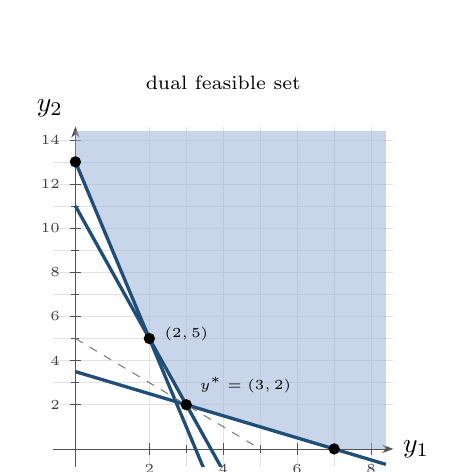
\begin{tikzpicture}
          \begin{axis}[geoaxis, xmin=-0.6, xmax=8.6, ymin=-0.8, ymax=14.6,
              xtick={2,4,6,8}, ytick={2,4,6,8,10,12,14},
              xlabel={$y_{1}$}, ylabel={$y_{2}$},
              title={dual feasible set}]
            \addplot[draw=none, name path=lA, domain=0:2, samples=2]{13-4*x};
            \addplot[draw=none, name path=uA, domain=0:2, samples=2]{14.4};
            \region{lA}{uA}{}
            \addplot[draw=none, name path=lB, domain=2:3, samples=2]{11-3*x};
            \addplot[draw=none, name path=uB, domain=2:3, samples=2]{14.4};
            \region{lB}{uB}{}
            \addplot[draw=none, name path=lC, domain=3:7, samples=2]{(7-x)/2};
            \addplot[draw=none, name path=uC, domain=3:7, samples=2]{14.4};
            \region{lC}{uC}{}
            \addplot[draw=none, name path=lD, domain=7:8.4, samples=2]{0};
            \addplot[draw=none, name path=uD, domain=7:8.4, samples=2]{14.4};
            \region{lD}{uD}{}
            \addplot[domain=0:4.2, samples=2]{11-3*x};
            \addplot[domain=0:8.4, samples=2]{(7-x)/2};
            \addplot[domain=0:3.5, samples=2]{13-4*x};
            \addplot[gray, dashed, thin, domain=0:5, samples=2]{5-x};
            \addplot[only marks, mark=*, mark size=1.4pt, black, forget plot]
              coordinates {(0,13) (2,5) (3,2) (7,0)};
            \node[font=\tiny, anchor=south west] at (axis cs:3.1,2.1) {$y^{*}=(3,2)$};
            \node[font=\tiny, anchor=west] at (axis cs:2.15,5.2) {$(2,5)$};
          \end{axis}
        \end{tikzpicture}
        \hfill\null
        \gcap{The dual feasible set (shaded, unbounded upwards) and the
        lowest iso-cost line $y_{1}+y_{2}=5$ (dashed) through $y^{*}=(3,2)$.}
        \end{gallery}

        (b)~At $y^{*}=(3,2)$ the third dual constraint is slack
        ($4\cdot3+2=14>13$), so $x_{3}^{*}=0$. Both $y_{i}^{*}>0$, so both
        primal rows bind:
        \[
          3x_{1}+2x_{2}=60,\qquad x_{1}+4x_{2}=60 .
        \]
        From the second, $x_{1}=60-4x_{2}$; substituting,
        $180-12x_{2}+2x_{2}=60$, so $x_{2}=12$ and $x_{1}=12$. Both are
        nonnegative, and
        $Z^{*}=11\cdot12+14\cdot12=132+168=300=W^{*}$. $\checkmark$

        (c)~Products $1$ and $2$ are made, $12$ units each; product~3 is
        not made. Both resources are used up completely ($36+24=60$,
        $12+48=60$), which fits their positive shadow prices: nothing is
        left over. One unit of product~3 uses $4$ machine hours and $1$
        labour hour, worth $4\cdot3+1\cdot2=14$ at shadow prices; its
        margin $13$ must rise above $14$ before it is worth producing.

        (d)~$t_{j}=(A^{\top}y^{*})_{j}-c_{j}$:
        $t_{1}=11-11=0$, $t_{2}=14-14=0$, $t_{3}=14-13=1$. Products $1$
        and $2$ break even exactly at shadow prices (and are made);
        product~3 falls short by $1$ per unit, which is the margin
        increase it needs.

  \item The dual is
        \[
          \min\; W=20y_{1}+90y_{2}
          \quad\text{s.t.}\quad
          y_{1}+3y_{2}\ge 4,\qquad 2y_{1}+y_{2}\ge 6,\qquad
          y_{1}+2y_{2}\ge 5,\qquad y\ge 0 .
        \]
        Corners of the feasible set: on the $y_{2}$-axis the binding line
        is the second ($y_{2}\ge 6$), giving $(0,6)$; the second and third
        lines meet at $2y_{1}+y_{2}=6$, $y_{1}+2y_{2}=5$, i.e.\
        $(\tfrac73,\tfrac43)$ (and $\tfrac73+4=\tfrac{19}{3}\ge 4$); on the
        $y_{1}$-axis the binding line is the third ($y_{1}\ge 5$), giving
        $(5,0)$. (The first line is cut off everywhere: for example its
        crossing with the second line, $(\tfrac{14}{5},\tfrac25)$, violates
        the third.) Values:
        \[
          W(0,6)=540,\qquad W(\tfrac73,\tfrac43)=\tfrac{140}{3}+120
          =\tfrac{500}{3},\qquad W(5,0)=100 .
        \]
        So $y^{*}=(5,0)$, $W^{*}=100$.

        Complementary slackness: at $(5,0)$ the first dual constraint is
        slack ($5>4$, $t_{1}=1$) and so is the second ($10>6$, $t_{2}=4$),
        hence $x_{1}^{*}=x_{2}^{*}=0$. Since $y_{1}^{*}=5>0$, resource~A
        binds: $x_{3}=20$. Since $y_{2}^{*}=0$, resource~B may have slack:
        $2\cdot20=40\le 90$, slack $50$. So $x^{*}=(0,0,20)$ and
        $Z^{*}=5\cdot20=100=W^{*}$. $\checkmark$

        Only product~3 is made ($20$ units). Resource~A is used up;
        $50$ units of resource~B are left over, which is why B's shadow
        price is $0$. Product~1 would need a margin above
        $1\cdot5=5$, i.e.\ $1$ more; product~2 above $2\cdot5=10$, i.e.\
        $4$ more: exactly the dual slacks.

  \item (a)~A min problem with $\ge$ rows and $x\ge 0$ has a max dual with
        $\le$ rows and $u\ge 0$:
        \[
          \max\; W=4u_{1}+4u_{2}+5u_{3}
          \quad\text{s.t.}\quad
          u_{1}+u_{2}+2u_{3}\le 3,\qquad u_{1}+3u_{2}+u_{3}\le 2,\qquad
          u\ge 0 .
        \]
        Its right-hand sides are the costs $3$ and $2$, both
        nonnegative, so it is a standard maximum problem: the origin is
        feasible and the slacks $t_{1},t_{2}$ form the first basis.

        (b)~Initial tableau:
        \begin{center}
        \begin{tabular}{c|ccccc|c}
        Basis & $u_{1}$ & $u_{2}$ & $u_{3}$ & $t_{1}$ & $t_{2}$ & RHS\\
        \hline
        $t_{1}$ & $1$ & $1$ & $2$ & $1$ & $0$ & $3$\\
        $t_{2}$ & $1$ & $3$ & $1$ & $0$ & $1$ & $2$\\
        \hline
        $W$ & $-4$ & $-4$ & $-5$ & $0$ & $0$ & $0$\\
        \end{tabular}
        \end{center}
        \emph{Iteration 1.} Pivot column $u_{3}$ ($-5$). Ratios:
        $3/2=1.5$, $2/1=2$; $t_{1}$ leaves, pivot element $2$. Row
        operations: $R_{1}\to R_{1}/2$; then $R_{2}\to R_{2}-R_{1}$,
        $R_{W}\to R_{W}+5R_{1}$.
        \begin{center}
        \begin{tabular}{c|ccccc|c}
        Basis & $u_{1}$ & $u_{2}$ & $u_{3}$ & $t_{1}$ & $t_{2}$ & RHS\\
        \hline
        $u_{3}$ & $\tfrac12$ & $\tfrac12$ & $1$ & $\tfrac12$ & $0$ & $\tfrac32$\\
        $t_{2}$ & $\tfrac12$ & $\tfrac52$ & $0$ & $-\tfrac12$ & $1$ & $\tfrac12$\\
        \hline
        $W$ & $-\tfrac32$ & $-\tfrac32$ & $0$ & $\tfrac52$ & $0$ & $\tfrac{15}{2}$\\
        \end{tabular}
        \end{center}
        \emph{Iteration 2.} Tie between $u_{1}$ and $u_{2}$; take $u_{1}$.
        Ratios: $R_{1}$: $\tfrac32\big/\tfrac12=3$; $R_{2}$:
        $\tfrac12\big/\tfrac12=1$; $t_{2}$ leaves, pivot element
        $\tfrac12$. Row operations: $R_{2}\to 2R_{2}$; then
        $R_{1}\to R_{1}-\tfrac12R_{2}$, $R_{W}\to R_{W}+\tfrac32R_{2}$.
        \begin{center}
        \begin{tabular}{c|ccccc|c}
        Basis & $u_{1}$ & $u_{2}$ & $u_{3}$ & $t_{1}$ & $t_{2}$ & RHS\\
        \hline
        $u_{3}$ & $0$ & $-2$ & $1$ & $1$ & $-1$ & $1$\\
        $u_{1}$ & $1$ & $5$ & $0$ & $-1$ & $2$ & $1$\\
        \hline
        $W$ & $0$ & $6$ & $0$ & $1$ & $3$ & $9$\\
        \end{tabular}
        \end{center}
        No negative entry: optimal, $u^{*}=(1,0,1)$, $W^{*}=9$.

        (c)~The primal optimum stands in the $W$-row under the dual's slack
        columns: $x_{1}^{*}=1$ (under $t_{1}$), $x_{2}^{*}=3$ (under
        $t_{2}$), with minimal cost $C^{*}=W^{*}=9$; check
        $3\cdot1+2\cdot3=9$. The entries under $u_{1},u_{2},u_{3}$ are the
        primal surpluses $0$, $6$, $0$: the first and third requirements
        are met exactly ($1+3=4$, $2+3=5$), the second is over-fulfilled
        by $6$ ($1+9=10\ge 4$).

        (d)~Complementary slackness: the second requirement has surplus
        $6$, so $u_{2}=0$; $x_{1},x_{2}>0$ make both dual constraints
        equations: $u_{1}+2u_{3}=3$ and $u_{1}+u_{3}=2$, hence
        $u_{3}=1$, $u_{1}=1$. Both nonnegative, and
        $W=4+5=9=C^{*}$. $\checkmark$

  \item (a)~Sign rules for a max primal: labour and machine ($\le$) give
        $y_{1},y_{2}\ge 0$; the contract ($\ge$) gives $y_{3}\le 0$; the
        variables $x_{1},x_{2}\ge 0$ give $\ge$ dual constraints:
        \[
          \min\; W=10y_{1}+16y_{2}+6y_{3}
          \quad\text{s.t.}\quad
          y_{1}+2y_{2}\ge 5,\qquad y_{1}+y_{2}+y_{3}\ge 4,
        \]
        with $y_{1},y_{2}\ge 0$, $y_{3}\le 0$.

        (b)~At $x^{*}=(4,6)$: labour $4+6=10$ (binds), machine
        $8+6=14<16$ (slack $2$, so $y_{2}=0$), contract $x_{2}=6$ (binds).
        Both variables are positive, so both dual constraints are
        equations:
        \[
          y_{1}+2\cdot0=5\;\Rightarrow\;y_{1}=5,\qquad
          5+0+y_{3}=4\;\Rightarrow\;y_{3}=-1 .
        \]
        Signs: $y_{1}=5\ge 0$, $y_{2}=0$, $y_{3}=-1\le 0$, all as
        required, and both dual constraints hold. Values:
        $W=50+0-6=44$ and $Z^{*}=20+24=44$. $\checkmark$

        (c)~$y_{3}=-1$: every additional unit the contract demands lowers
        the maximal profit by $1$. Product~2 earns $4$ per unit but uses a
        labour hour that is worth $y_{1}=5$ in product~1, so forcing one
        more unit of it costs $5-4=1$. Check with a contract of $7$:
        labour and contract binding give $x=(3,7)$, machine $6+7=13\le 16$,
        and $Z=15+28=43=44-1$. $\checkmark$

        (d)~Written as $-x_{2}\le -6$, the row is of type $\le$ and gets a
        dual variable $\ge 0$; it is the old one with the sign flipped,
        $+1$. Read: raising the right-hand side $-6$ by one unit (to $-5$,
        a contract of $5$ units) raises $Z^{*}$ by $1$.

  \item (a)~Sign rules for a min primal: the $\ge$ rows give
        $u_{1},u_{3}\ge 0$, the $\le$ row gives $u_{2}\le 0$; the
        variables $x_{j}\ge 0$ give $\le$ dual constraints:
        \[
          \max\; W=8u_{1}+4u_{2}-10u_{3}
          \quad\text{s.t.}\quad
          u_{1}+u_{2}+u_{3}\le 2,\qquad 2u_{1}-3u_{3}\le 5,
        \]
        with $u_{1}\ge 0$, $u_{2}\le 0$, $u_{3}\ge 0$.

        (b)~At $x^{*}=(4,2)$: $4+4=8$ (binds), $x_{1}=4$ (binds),
        $4-6=-2>-10$ (surplus $8$, so $u_{3}=0$). Both variables are
        positive, so both dual constraints are equations:
        \[
          2u_{1}=5\;\Rightarrow\;u_{1}=\tfrac52,\qquad
          \tfrac52+u_{2}=2\;\Rightarrow\;u_{2}=-\tfrac12 .
        \]
        Signs: $u_{1}\ge 0$, $u_{2}\le 0$, $u_{3}=0$, all as required.
        Values: $W=8\cdot\tfrac52+4\cdot(-\tfrac12)-0=20-2=18$ and
        $C^{*}=8+10=18$. $\checkmark$

        (c)~$u_{1}=\tfrac52$: one more unit of the requirement raises the
        minimal cost by $2.5$ (it is met at the margin by $x_{2}$, which
        delivers $2$ units for $5$). $u_{2}=-\tfrac12$: one more unit of
        capacity for input~1 lowers the cost by $0.5$, because a unit of
        $x_{1}$ replaces half a unit of $x_{2}$: it saves $2.5$ and costs
        $2$. $u_{3}=0$: the third row has surplus, so its (negative)
        right-hand side is irrelevant at the margin. Check with
        $x_{1}\le 5$: $x=(5,1.5)$ satisfies $5+3=8$ and $5-4.5\ge -10$,
        and $C=10+7.5=17.5=18-0.5$. $\checkmark$

  \item (a)~$\mathcal{L}=3x_{1}+2x_{2}+\lambda_{1}(4-x_{1}-x_{2})
        +\lambda_{2}(6-2x_{1}-x_{2})$.

        (b)~With $x\ge 0$:
        \[
          \begin{aligned}
            &\pd{\mathcal{L}}{x_{1}}=3-\lambda_{1}-2\lambda_{2}\le 0,\quad
             x_{1}\ge 0,\quad x_{1}(3-\lambda_{1}-2\lambda_{2})=0,\\
            &\pd{\mathcal{L}}{x_{2}}=2-\lambda_{1}-\lambda_{2}\le 0,\quad
             x_{2}\ge 0,\quad x_{2}(2-\lambda_{1}-\lambda_{2})=0,\\
            &4-x_{1}-x_{2}\ge 0,\quad \lambda_{1}\ge 0,\quad
             \lambda_{1}(4-x_{1}-x_{2})=0,\\
            &6-2x_{1}-x_{2}\ge 0,\quad \lambda_{2}\ge 0,\quad
             \lambda_{2}(6-2x_{1}-x_{2})=0 .
          \end{aligned}
        \]
        (c)~At $x=(2,2)$, $\lambda=(1,1)$: $3-1-2=0$ and $2-1-1=0$ (so
        both products vanish); $4-4=0$ and $6-6=0$ (both rows bind, so
        both products vanish); all signs hold. Every condition is
        satisfied, and $Z=6+4=10$.

        (d)~$\partial\mathcal{L}/\partial x_{j}\le 0$ is
        $\lambda_{1}+2\lambda_{2}\ge 3$, $\lambda_{1}+\lambda_{2}\ge 2$,
        the dual constraints of Solution~1 with $\lambda$ in place of $y$;
        $\lambda\ge 0$ is the dual sign condition; the rows
        $\partial\mathcal{L}/\partial\lambda_{i}\ge 0$ are primal
        feasibility; the four product conditions are complementary
        slackness. So the multipliers are the dual solution
        $y^{*}=(1,1)$, i.e.\ the shadow prices. The objective is linear
        (concave) and the constraints are linear, so the Kuhn--Tucker
        conditions are sufficient: $(2,2)$ is optimal, as Solution~14
        found from the tableau.

  \item With $x_{j}\ge 0$ written as $-x_{j}\le 0$ and multiplier
        $\mu_{j}\ge 0$:
        \[
          \mathcal{L}=11x_{1}+14x_{2}+13x_{3}
          +\lambda_{1}(60-3x_{1}-2x_{2}-4x_{3})
          +\lambda_{2}(60-x_{1}-4x_{2}-x_{3})
          +\mu_{1}x_{1}+\mu_{2}x_{2}+\mu_{3}x_{3} .
        \]
        Stationarity at $\lambda=(3,2)$, $\mu=(0,0,1)$:
        \[
          \begin{aligned}
            \pd{\mathcal{L}}{x_{1}}&=11-3\lambda_{1}-\lambda_{2}+\mu_{1}
              =11-9-2+0=0,\\
            \pd{\mathcal{L}}{x_{2}}&=14-2\lambda_{1}-4\lambda_{2}+\mu_{2}
              =14-6-8+0=0,\\
            \pd{\mathcal{L}}{x_{3}}&=13-4\lambda_{1}-\lambda_{2}+\mu_{3}
              =13-12-2+1=0 .
          \end{aligned}
        \]
        Primal feasibility at $x=(12,12,0)$: $36+24=60\le 60$,
        $12+48=60\le 60$, $x\ge 0$. Signs: $\lambda,\mu\ge 0$.
        Complementary slackness: both rows bind, so
        $\lambda_{i}(60-\dots)=0$; $\mu_{1}x_{1}=0\cdot12=0$,
        $\mu_{2}x_{2}=0\cdot12=0$, $\mu_{3}x_{3}=1\cdot0=0$. All conditions
        hold, so the point is optimal (with $Z=300$). Interpretation:
        $\mu_{3}=(4\lambda_{1}+\lambda_{2})-13=1$ is the dual slack $t_{3}$
        of Additional Solution~9: the multiplier of the sign constraint
        $x_{3}\ge 0$ measures how much the profit would drop per unit if
        product~3 were forced into the plan, i.e.\ the margin it lacks.

  \item (a)~\textbf{False.} $t_{2}=4$: the margin must rise by more than
        $4$, to above $10=2y_{1}^{*}$. At $9$ the product still uses
        $2$ units of resource~A worth $10$ and earns only $9$.

        (b)~\textbf{True.} $t_{1}=1$, and a rise of $1.5>1$ lifts the
        margin to $5.5$, above the opportunity cost $1\cdot y_{1}^{*}=5$:
        the product now prices out positive ($5.5-5=0.5>0$), so the
        current plan is no longer optimal and product~1 enters.

        (c)~\textbf{False.} $t_{3}=0$ only says that product~3 breaks even
        at the current shadow prices, which it must, since it is made. Its
        margin sets the price $y_{1}^{*}=c_{3}$; if $c_{3}$ falls below
        $4$, product~1 earns more per unit of resource~A ($4$ against
        $c_{3}$), and the plan switches to product~1.

        (d)~\textbf{True.} The $z$-row entry under $x_{j}$ in the end
        tableau is $(A^{\top}y^{*})_{j}-c_{j}=t_{j}$, and the reduced cost
        is $c_{j}-(A^{\top}y^{*})_{j}=-t_{j}$; for basic variables both
        are $0$.
\end{solutions}

\chapter{Sensitivity Analysis and Interpreting Computer Output}

An LP is rarely solved once and filed away. Prices shift, capacities are
renegotiated, new products are proposed: and the first question is always
the same: does the old plan survive, and what is the change worth?
Sensitivity analysis answers such what-if
questions \emph{from the solved problem alone}, without starting the simplex
method over. Every serious solver prints the answers in a standard
\emph{sensitivity report}, and reading that
report (the interpretation of a computer solution) is a skill tested in its
own right. This chapter builds the report line by line from the machinery
of Chapters~4--7: the end tableau supplies the numbers, duality explains
what they mean.

\section{Core Rules}

\begin{rulebox}{Setting}
Throughout, the primal is a maximisation in resource form:
\[
  \max\; z=c_{1}x_{1}+\dots+c_{n}x_{n}
  \quad\text{s.t.}\quad
  \sum_{j=1}^{n}a_{ij}x_{j}\le b_{i}\;(i=1,\dots,m),\qquad x_{j}\ge 0 .
\]
It has been solved: the optimal plan is $x^{*}$ with value $z^{*}$, and the
optimal dual solution (shadow prices) is $y^{*}=(y_{1},\dots,y_{m})$.
Sensitivity analysis asks how $x^{*}$ and $z^{*}$ react when a single piece
of data (one $b_{i}$ or one $c_{j}$) is changed. Minimum problems and
$\ge$ rows are handled by measuring every change as an \emph{improvement}
of the objective; the boxes on the classic report layout below show how.
\end{rulebox}

\begin{rulebox}{Shadow price and RHS ranging}
The shadow price $y_{i}$ is the rate of change of the
optimal value with respect to capacity $i$:
\[
  \Delta z^{*} \;=\; y_{i}\,\Delta b_{i},
\]
valid as long as the change leaves the \emph{same set of constraints
binding} (the same optimal basis). The interval of $b_{i}$-values for which
this holds is the \emph{validity range}, reported as an allowable increase
and an allowable decrease around the current $b_{i}$. Inside the range the
\emph{plan} $x^{*}$ moves (the basic variables are recomputed), but the
list of binding constraints (and hence every shadow price) stays the
same. Outside the range the basis changes and the report makes no promise.
For a \emph{nonbinding} constraint: $y_{i}=0$, the allowable decrease
equals the slack, and the allowable increase is $\infty$.
\end{rulebox}

\begin{rulebox}{RHS ranging by hand (two variables)}
If the optimum is the corner where constraints $r$ and $s$ bind, replace
$b_{r}$ by a parameter and re-solve the $2\times 2$ system of the two
binding constraints. The corner coordinates become linear functions of
$b_{r}$. The validity range is the set of $b_{r}$ for which
\begin{itemize}[leftmargin=1.6em,itemsep=0.3ex]
  \item both coordinates stay $\ge 0$, and
  \item every other constraint is still satisfied.
\end{itemize}
On this range $z^{*}(b_{r})$ is linear with slope $y_{r}$.
\end{rulebox}

\begin{rulebox}{Objective-coefficient ranging}
Changing a coefficient $c_{j}$ tilts the iso-profit lines but moves no
constraint: the feasible region is unchanged. The current corner stays
optimal as long as the iso-profit slope stays between the slopes of the two
constraints binding there. For a corner of
$a_{11}x_{1}+a_{12}x_{2}\le b_{1}$ and $a_{21}x_{1}+a_{22}x_{2}\le b_{2}$
(slopes $m_{1}\le m_{2}$, both negative) the condition is
\[
  m_{1}\;\le\;-\frac{c_{1}}{c_{2}}\;\le\;m_{2}.
\]
Fixing one coefficient and solving for the other yields its allowable
increase and decrease. Inside the range the plan $x^{*}$ is unchanged and
\[
  \Delta z^{*}\;=\;x_{j}^{*}\,\Delta c_{j}.
\]
At an endpoint of the range two corners are optimal simultaneously
(multiple optima); beyond it the optimum jumps to a neighbouring corner.
\end{rulebox}

\begin{rulebox}{Reduced cost}
The reduced cost of a variable $x_{j}$ is
\[
  r_{j} \;=\; c_{j}-\sum_{i=1}^{m}a_{ij}\,y_{i}
  \;=\;\text{own margin}\;-\;\text{opportunity cost of the resources used}.
\]
At a maximum every $r_{j}\le 0$; basic (produced) variables have
$r_{j}=0$; a nonbasic variable has $r_{j}\le 0$, and $|r_{j}|$ is exactly
how much its objective coefficient must \emph{improve} before producing it
becomes worthwhile. Equivalently: $c_{j}$ may rise by $|r_{j}|$ before the
current plan changes, while any decrease of $c_{j}$ leaves an unproduced
product unproduced. The same formula prices out a \emph{new} product: it
enters the plan if and only if its margin exceeds
$\sum_{i}a_{ij}\,y_{i}$, the value of the capacity it would consume.
\end{rulebox}

\begin{rulebox}{Reading a solver sensitivity report}
Solvers print two blocks. The \textbf{variable block} has one row per
decision variable:
\begin{itemize}[leftmargin=1.6em,itemsep=0.3ex]
  \item \emph{Final value}: the optimal $x_{j}^{*}$;
  \item \emph{Reduced cost}: $r_{j}$ ($0$ for produced variables);
  \item \emph{Objective coefficient} with \emph{allowable increase /
        decrease}: the range of $c_{j}$ over which the plan $x^{*}$ is
        unchanged.
\end{itemize}
The \textbf{constraint block} has one row per constraint:
\begin{itemize}[leftmargin=1.6em,itemsep=0.3ex]
  \item \emph{Final value}: the left-hand side $\sum_{j}a_{ij}x_{j}^{*}$
        (equal to $b_{i}$ exactly when the constraint binds);
  \item \emph{Shadow price}: $y_{i}$;
  \item \emph{Constraint RHS} with \emph{allowable increase / decrease}:
        the range of $b_{i}$ over which $y_{i}$ stays valid.
\end{itemize}
The entry \texttt{1E+30} is solver notation for $\infty$: no finite limit.
\end{rulebox}

\begin{rulebox}{The classic report layout: dual prices and sign conventions}
Many solvers print a plain-text report instead of a spreadsheet. The
objective counts as row~1, so the constraints are rows $2,3,\dots$
\begin{itemize}[leftmargin=1.6em,itemsep=0.3ex]
  \item \texttt{OBJECTIVE FUNCTION VALUE}: $z^{*}$, or $C^{*}$ for a
        minimum problem.
  \item \texttt{VALUE} and \texttt{REDUCED COST}: $x_{j}^{*}$, and the
        amount by which the objective coefficient of $x_{j}$ would have to
        \emph{improve} (rise in a max problem, fall in a min problem)
        before $x_{j}$ becomes positive. It is printed as a nonnegative
        number and is $0$ for basic variables.
  \item \texttt{SLACK OR SURPLUS}: $b_{i}-a_{i}^{\top}x^{*}$ for a $\le$
        row, $a_{i}^{\top}x^{*}-b_{i}$ for a $\ge$ row; never negative, and
        $0$ exactly when the row binds.
  \item \texttt{DUAL PRICES}: the \emph{improvement} of the objective per
        unit increase of $b_{i}$, that is $\partial z^{*}/\partial b_{i}$
        for a max problem and $-\partial C^{*}/\partial b_{i}$ for a min
        problem.
  \item \texttt{RANGES IN WHICH THE BASIS IS UNCHANGED}: current
        coefficient or right-hand side with allowable increase and
        decrease; \texttt{INFINITY} means no limit.
\end{itemize}
\textbf{Sign rule.} Because improvement is measured the same way for both
senses, the sign of a dual price depends on the row type only: raising
$b_{i}$ loosens a $\le$ row, so its dual price is $\ge 0$; it tightens a
$\ge$ row, so its dual price is $\le 0$; an equality row can have either
sign. Link to Chapter~7: for a max problem the dual price is $y_{i}$; for
a min problem it is $-u_{i}$, where $u_{i}=\partial C^{*}/\partial b_{i}$
is the dual variable of the min problem. Rewriting $\min C$ as
$\max\,(-C)$ leaves every dual price and reduced cost unchanged and only
flips the sign of the objective value.
\end{rulebox}

\begin{rulebox}{Filling the gaps in an incomplete report}
\begin{enumerate}[leftmargin=1.8em,itemsep=0.3ex]
  \item \textbf{Variables.} Reduced cost $>0$: the variable is nonbasic,
        \texttt{VALUE} $=0$. Reduced cost $0$: normally basic (a
        nonbasic variable with reduced cost $0$ signals alternative
        optima). A nonbasic variable also shows a one-sided objective
        range: the improving side equals its reduced cost, the other side
        is \texttt{INFINITY}.
  \item \textbf{Rows.} Slack $0$ or a nonzero dual price: the row binds. A
        nonbinding row has dual price $0$ and a one-sided right-hand-side
        range: \texttt{INFINITY} on its loosening side, and on the other
        side its slack (allowable decrease of a $\le$ row) or surplus
        (allowable increase of a $\ge$ row). The converse can fail, since
        a binding row may also show \texttt{INFINITY} on one side; when
        the slack is blank, count: a nondegenerate optimum has exactly as
        many positive basic variables as there are rows.
  \item \textbf{Primal.} Set the nonbasic variables to $0$, solve the
        binding rows for the basic ones, then compute the missing slacks
        and the objective value.
  \item \textbf{Dual.} Write the dual of the LP as stated (sign rules of
        Chapter~7). Nonbinding rows get dual value $0$; the dual
        constraint of every basic variable becomes an equation. Solve, check
        the signs, and check that the dual slack of each nonbasic variable
        equals its printed reduced cost.
  \item \textbf{Report and certify.} Convert to dual prices ($y_{i}$ for
        max, $-u_{i}$ for min) and confirm $W^{*}=Z^{*}$: a feasible
        primal--dual pair with equal values is optimal.
\end{enumerate}
\end{rulebox}

\begin{rulebox}{Rebuilding the end tableau from a report}
Bring the LP to maximum form with $\le$ rows ($\min C$ becomes
$\max\,(-C)$, each $\ge$ row is multiplied by $-1$), with slack $s_{i}$ in
row~$i$. Then:
\begin{itemize}[leftmargin=1.6em,itemsep=0.3ex]
  \item \textbf{basis:} the variables with positive value and the slacks
        of the rows with positive slack or surplus ($m$ in total; if fewer,
        the optimum is degenerate and zero-valued basic variables complete
        the basis);
  \item \textbf{RHS column:} their values; bottom right: $z^{*}$ (for a
        min problem $-C^{*}$);
  \item \textbf{$z$-row:} under $x_{j}$ its reduced cost; under $s_{i}$
        the dual price of row~$i$ in $\le$ form, which is the printed dual
        price for an original $\le$ row and its negative for an original
        $\ge$ row; $0$ under every basic variable;
  \item \textbf{body:} the unit columns of the basic variables. The
        remaining entries form $B^{-1}A$; the report does not contain
        them, and they can be computed only from the model itself.
\end{itemize}
\end{rulebox}

\begin{rulebox}{What-if questions without re-solving}
Assume resource costs are already counted in the margins $c_{j}$. Then:
\begin{itemize}[leftmargin=1.6em,itemsep=0.3ex]
  \item \textbf{Buy more of resource $i$ at a premium $p$ per unit?}
        Worth it iff $p<y_{i}$; each unit nets $y_{i}-p$; guaranteed only
        up to the allowable increase of $b_{i}$.
  \item \textbf{Sell (rent out) a unit of resource $i$ at price $p$?}
        Worth it iff $p>y_{i}$; guaranteed up to the allowable decrease.
  \item \textbf{Launch a new product with margin $m$ using $a_{i}$ units
        of resource $i$?} It enters the plan iff
        $m>\sum_{i}a_{i}y_{i}$.
  \item \textbf{A margin $c_{j}$ changes within its range?} Plan
        unchanged, $z^{*}$ changes by $x_{j}^{*}\,\Delta c_{j}$.
  \item \textbf{A capacity $b_{i}$ changes within its range?}
        $z^{*}$ changes by $y_{i}\,\Delta b_{i}$; the new plan follows
        from re-solving the binding equations only.
\end{itemize}
\end{rulebox}

\begin{rulebox}{Limits of the report; the 100\%-rule}
Every range in the report covers \emph{one} change at a time, all other
data held fixed. For several \emph{simultaneous} changes (all among the
$c_{j}$, or all among the $b_{i}$) the 100\%-rule gives a quick sufficient check: express each
change as a fraction of its allowable increase or decrease; if the
fractions sum to at most $1$ (i.e.\ $100\%$), the report's conclusions
remain valid. If the sum exceeds $1$ the rule is silent: the basis
\emph{may} have changed, and only re-solving settles it. The rule is
sufficient, not necessary.
\end{rulebox}

\begin{rulebox}{Beyond the allowable range: what can still be said}
Measure the objective as improvement ($z^{*}$ for a max problem, $-C^{*}$
for a min problem). As a function of one right-hand side $b_{i}$, all
other data fixed, the optimal improvement is piecewise linear and
\emph{concave}: on the validity range its slope is the dual price $y_{i}$,
and the slope can only fall as $b_{i}$ grows and only rise as $b_{i}$
falls. So for a change that exceeds the allowable increase $I$ or decrease
$D$:
\begin{itemize}[leftmargin=1.6em,itemsep=0.3ex]
  \item the part of the change inside the range is exact: $+y_{i}I$ for
        the first $I$ units of an increase, $-y_{i}D$ for the first $D$
        units of a decrease;
  \item an increase by $\Delta>I$ improves the objective by \emph{at most}
        $y_{i}\Delta$ in total: every unit beyond the range is worth at
        most $y_{i}$;
  \item a decrease by $\Delta>D$ worsens it by \emph{at least}
        $y_{i}\Delta$: every unit beyond the range costs at least $y_{i}$
        (and the LP may even become infeasible);
  \item loosening a row never hurts, so for a $\le$ row an increase
        beyond $I$ still yields at least the exact gain $y_{i}I$.
\end{itemize}
For an objective coefficient the old plan stays feasible, so
$z^{*}+x_{j}^{*}\Delta c_{j}$ is always a \emph{lower} bound for the new
maximum (and $C^{*}+x_{j}^{*}\Delta c_{j}$ an \emph{upper} bound for a new
minimum), inside the range with equality, outside it as a bound.
\end{rulebox}

\section{Worked Examples}

\begin{worked}{Sensitivity analysis on the running example: how far can $100$ machine hours and the profit $40$ move before the answer changes?}
\wstep{Step 1. Recall what stays fixed.}
From Chapter~5 the optimal basis is $\{x_{1},x_{2}\}$ with
\[
  B=\begin{pmatrix}2&1\\1&1\end{pmatrix},
  \qquad
  B^{-1}=\begin{pmatrix}1&-1\\-1&2\end{pmatrix},
  \qquad
  \mathbf y=(10,20) .
\]
Sensitivity analysis asks: over what range of a parameter does this
\emph{basis} remain optimal? Within that range the answer changes smoothly
and predictably; outside it, a different basis takes over and everything
must be recomputed.

\wstep{Step 2. Right-hand-side ranging for machine hours $b_{1}$.}
The basic variables are $\mathbf x_{B}=B^{-1}\mathbf b$:
\[
  \begin{pmatrix}x_{1}\\x_{2}\end{pmatrix}
  =\begin{pmatrix}1&-1\\-1&2\end{pmatrix}\begin{pmatrix}b_{1}\\80\end{pmatrix}
  =\begin{pmatrix}b_{1}-80\\160-b_{1}\end{pmatrix}.
\]
Feasibility requires both to be $\ge0$:
\[
  b_{1}-80\ge0\ \text{and}\ 160-b_{1}\ge0
  \quad\Longrightarrow\quad
  \boxed{80\le b_{1}\le160 .}
\]
At $b_{1}=100$ this gives $(20,60)$ \checkmark, comfortably inside.

\wstep{Step 3. What the range means.}
\emph{Within} $[80,160]$ the shadow price $10$ is exact: each additional
machine hour is worth $10$ euros. Ten more hours, $b_{1}=110$, gives
$z=2600+10\cdot10=2700$ and the plan $(30,50)$ --- check:
$2(30)+50=110$ \checkmark and $30+50=80$ \checkmark, with
$z=1200+1500=2700$ \checkmark.

\emph{Outside} it the price changes. At $b_{1}=160$, $x_{2}$ hits zero;
beyond that, extra machine hours cannot be used because labour has run out,
and the shadow price drops to $0$.
\wtrap{Shadow prices are local. Applying $10$ euros per hour to a proposal
for $200$ machine hours predicts $z=3600$; the truth is that nothing beyond
$160$ has any value, so $z$ stops at $3200$. Always quote the range with the
price, and never extrapolate past it.}

\wstep{Step 4. Objective-coefficient ranging for $c_{1}=40$.}
Optimality requires the $z$-row entries under the non-basic variables
(the slacks) to stay non-negative. Those entries are
$\mathbf y^{\!\top}=\mathbf c_{B}^{\!\top}B^{-1}$:
\[
  (c_{1},30)\begin{pmatrix}1&-1\\-1&2\end{pmatrix}
  =\bigl(c_{1}-30,\;-c_{1}+60\bigr).
\]
\[
  c_{1}-30\ge0\ \text{and}\ 60-c_{1}\ge0
  \quad\Longrightarrow\quad
  \boxed{30\le c_{1}\le60 .}
\]

\wstep{Step 5. Confirm it geometrically.}
The objective's slope is $-c_{1}/30$. The corner $(20,60)$ stays optimal as
long as that slope lies between the slopes of the two binding constraints,
$-2$ (machine) and $-1$ (labour):
\[
  -2\le-\frac{c_{1}}{30}\le-1
  \quad\Longrightarrow\quad
  30\le c_{1}\le60 . \checkmark
\]
At the endpoints the objective becomes parallel to one of the constraints
and multiple optima appear --- precisely the situation of Chapter~6.
\wtrap{Within this range the optimal \emph{plan} $(20,60)$ does not change
at all; only the optimal \emph{value} does, at $20$ euros per unit of
$c_{1}$. Right-hand-side changes move the plan and keep the price;
objective changes keep the plan and move the value. Confusing which is
which is the chapter's main hazard.}

\wstep{Step 6. Reduced costs, and the new-product question.}
Both $x_{1}$ and $x_{2}$ are basic, so both have reduced cost $0$: they are
already in the plan. A \emph{non-basic} variable's reduced cost says how
much its profit coefficient would have to improve before it enters. For the
hypothetical product~3 of Chapter~5 (one hour of each resource, margin
$35$):
\[
  35-\mathbf y^{\!\top}\mathbf a_{3}=35-(10+20)=5>0 ,
\]
so it enters; at a margin of $28$ it would not, and the break-even margin is
exactly $30$.

\wstep{Step 7. Two parameters at once: the 100\% rule.}
Ranging is valid for \textbf{one change at a time}. For simultaneous
changes, add the fractions of each allowable range used up; if the total is
at most $100\%$, the basis certainly stays optimal. Raising $b_{1}$ from
$100$ to $130$ uses $30/60=50\%$ of its upward slack; a change in $b_{2}$
that uses $40\%$ of its own range brings the total to $90\%$, so the basis
survives. Above $100\%$ the rule is silent --- not violated, merely
uninformative, and re-solving is then the only reliable answer.

\wstep{Step 8. What a solver's sensitivity report contains.}
\begin{center}\footnotesize
\begin{tabular}{ll}
  \hline
  column & meaning\\
  \hline
  final value & the optimal $x_{j}$ or the constraint's usage\\
  reduced cost & $0$ if basic; else the margin shortfall\\
  shadow price & value of one more unit of that right-hand side\\
  allowable increase/decrease & the ranges computed above\\
  \hline
\end{tabular}
\end{center}
Every number in such a report has been derived by hand in this example. The
report is not a black box --- it is this chapter, printed.
\end{worked}

\begin{worked}{Complete an incomplete classic-layout report for a minimum problem, certify it, and rebuild the end tableau}
The LP and the solver's report, with the blanks still to be filled:
\[
  \min\; C=4x_{1}-2x_{2}-5x_{3}
  \quad\text{s.t.}\quad
  \begin{array}{rcrl}
    x_{1}-x_{2} &\ge& -3 & \text{(row 2)}\\
    x_{1}+2x_{2}+2x_{3} &\le& 12 & \text{(row 3)}\\
    2x_{2}-x_{3} &\ge& -3 & \text{(row 4)}\\
    x_{3} &\le& 10 & \text{(row 5)}\\
    x_{1},x_{2},x_{3} &\ge& 0 .
  \end{array}
\]
\begin{center}\footnotesize\ttfamily
\begin{tabular}{lrr}
\multicolumn{3}{l}{OBJECTIVE FUNCTION VALUE\quad 1)\ \underline{\hspace{3em}}}\\[3pt]
VARIABLE & VALUE & REDUCED COST\\
X1 & \underline{\hspace{3em}} & 6.000000\\
X2 & \underline{\hspace{3em}} & 0.000000\\
X3 & \underline{\hspace{3em}} & 0.000000\\[3pt]
ROW & SLACK OR SURPLUS & DUAL PRICES\\
2) & \underline{\hspace{3em}} & \underline{\hspace{3em}}\\
3) & 0.000000 & \underline{\hspace{3em}}\\
4) & 0.000000 & \underline{\hspace{3em}}\\
5) & \underline{\hspace{3em}} & \underline{\hspace{3em}}\\
\end{tabular}

\medskip
\begin{tabular}{lrrr}
\multicolumn{4}{l}{OBJ COEFFICIENT RANGES}\\
VARIABLE & CURRENT COEF & ALLOWABLE INCREASE & ALLOWABLE DECREASE\\
X1 & 4.000000 & INFINITY & 6.000000\\
X2 & $-$2.000000 & 12.000000 & 3.000000\\
X3 & $-$5.000000 & 3.000000 & INFINITY\\[3pt]
\multicolumn{4}{l}{RIGHTHAND SIDE RANGES}\\
ROW & CURRENT RHS & ALLOWABLE INCREASE & ALLOWABLE DECREASE\\
2 & $-$3.000000 & 2.000000 & INFINITY\\
3 & 12.000000 & 12.000000 & 6.000000\\
4 & $-$3.000000 & 6.000000 & 3.000000\\
5 & 10.000000 & INFINITY & 5.000000\\
\end{tabular}
\end{center}

\wstep{Step 1. Can the LP be read as a standard maximum problem?}
Origin test: $0\ge -3$, $0\le 12$, $0\ge -3$, $0\le 10$ all hold. So it
can: maximise $-C=-4x_{1}+2x_{2}+5x_{3}$ subject to $-x_{1}+x_{2}\le 3$,
$x_{1}+2x_{2}+2x_{3}\le 12$, $-2x_{2}+x_{3}\le 3$, $x_{3}\le 10$. We need
this form in Step~10.

\wstep{Step 2. Fix what the columns mean before reading a single number.}
This is a \emph{minimum} problem, so a dual price is the decrease of the
cost per unit increase of the right-hand side, and a reduced cost is how far
a cost coefficient must \emph{fall}. Expected signs: rows 3 and 5 ($\le$)
can only have dual prices $\ge 0$, rows 2 and 4 ($\ge$) only $\le 0$.
\wtrap{A negative dual price in this layout is not an error and not a
``negative shadow price of a resource'': it is the normal sign of a
binding $\ge$ row, in a max problem and in a min problem alike.}

\wstep{Step 3. Which variables are basic?}
X1 has reduced cost $6>0$, so it is nonbasic: $x_{1}^{*}=0$. Its objective
range confirms it: decrease $6$ (the improving direction for a cost),
increase \texttt{INFINITY}. X2 and X3 have reduced cost $0$ and two-sided
ranges: basic.

\wstep{Step 4. Which rows bind?}
Rows 3 and 4 show slack $0$: binding. Rows 2 and 5 are blank, so count:
four rows mean four basic variables, $x_{2}$ and $x_{3}$ are two of them,
and (the optimum being nondegenerate) the other two are the slacks of
rows 2 and 5, which are therefore nonbinding. Their ranges fit this:
\texttt{INFINITY} on the loosening side, and on the other side the room
left. Row~2 ($\ge$) has allowable increase $2$, so its surplus should be
$2$; row~5 ($\le$) has allowable decrease $5$, so its slack should be $5$.
Step~5 confirms both.

\wstep{Step 5. Solve the primal.}
With $x_{1}=0$ the binding rows read
\[
  2x_{2}+2x_{3}=12,\qquad 2x_{2}-x_{3}=-3 .
\]
Subtracting: $3x_{3}=15$, so $x_{3}=5$ and $x_{2}=1$. Then
\[
  \text{row 2: } 0-1-(-3)=2\ \text{(surplus)},\qquad
  \text{row 5: } 10-5=5\ \text{(slack)},\qquad
  C^{*}=0-2-25=-27 .
\]
Both values agree with the ranges. \checkmark

\wstep{Step 6. Solve the dual by complementary slackness.}
By the sign rules for a min problem, the $\ge$ rows get $u_{1},u_{3}\ge 0$
and the $\le$ rows get $u_{2},u_{4}\le 0$:
\[
  \max\; W=-3u_{1}+12u_{2}-3u_{3}+10u_{4}
  \quad\text{s.t.}\quad
  \begin{array}{rcl}
    u_{1}+u_{2} &\le& 4\\
    -u_{1}+2u_{2}+2u_{3} &\le& -2\\
    2u_{2}-u_{3}+u_{4} &\le& -5 .
  \end{array}
\]
Rows 2 and 5 are slack, so $u_{1}=u_{4}=0$. $x_{2},x_{3}>0$ turn the
second and third dual constraints into equations:
\[
  2u_{2}+2u_{3}=-2,\qquad 2u_{2}-u_{3}=-5
  \quad\Longrightarrow\quad 3u_{3}=3,\; u_{3}=1,\; u_{2}=-2 .
\]
Signs: $u_{2}=-2\le 0$, $u_{3}=1\ge 0$. \checkmark\ The first dual
constraint: $u_{1}+u_{2}=-2\le 4$, slack $6$, which is exactly the printed
reduced cost of X1. \checkmark

\wstep{Step 7. Fill in the report.}
Dual price $=-u_{i}$ for a min problem:
\begin{center}\footnotesize\ttfamily
\begin{tabular}{lrr}
\multicolumn{3}{l}{OBJECTIVE FUNCTION VALUE\quad 1)\ $-$27.00000}\\[3pt]
VARIABLE & VALUE & REDUCED COST\\
X1 & 0.000000 & 6.000000\\
X2 & 1.000000 & 0.000000\\
X3 & 5.000000 & 0.000000\\[3pt]
ROW & SLACK OR SURPLUS & DUAL PRICES\\
2) & 2.000000 & 0.000000\\
3) & 0.000000 & 2.000000\\
4) & 0.000000 & $-$1.000000\\
5) & 5.000000 & 0.000000\\
\end{tabular}
\end{center}
The signs follow the rule of Step~2: $+2$ on the $\le$ row~3, $-1$ on the
$\ge$ row~4.

\wstep{Step 8. Certify optimality.}
$x^{*}=(0,1,5)$ satisfies every primal row, $u^{*}=(0,-2,1,0)$ every dual
row and sign condition, and
\[
  W=-3\cdot0+12\cdot(-2)-3\cdot1+10\cdot0=-27=C^{*} .
\]
By weak duality no feasible plan costs less than $-27$, so both solutions
are optimal.
\wtrap{The certificate needs the dual of the LP \emph{as stated}. Taking
the dual of the converted max form instead is fine too, but then all its
variables are $\ge 0$ and equal the $z$-row entries of Step~10; mixing the
two conventions is how sign errors creep in.}

\wstep{Step 9. Interpret two numbers.}
Reduced cost $6$ of X1: the cost coefficient $4$ would have to fall by more
than $6$, below $-2$, before $x_{1}$ enters the plan; equivalently, forcing
one unit of $x_{1}$ into the solution raises the minimal cost by $6$. Dual
price $-1$ of row~4: raising its right-hand side from $-3$ to $-2$ raises
the minimal cost by $1$, valid for $-6\le b_{4}\le 3$.

\wstep{Step 10. Rebuild the end tableau.}
In the max form of Step~1 with slacks $s_{1},\dots,s_{4}$ for rows 2--5,
the basis consists of the positive variables $x_{2},x_{3}$ and the slacks of
the nonbinding rows, $s_{1}=2$ and $s_{4}=5$. The $z$-row carries the
reduced costs under the structural columns and, under $s_{i}$, the printed
dual price for a $\le$ row or its negative for a $\ge$ row: $0$, $2$, $1$,
$0$. Bottom right: $-C^{*}=27$. A dot marks an entry the report does not
contain:
\begin{center}\footnotesize
\begin{tabular}{c|ccccccc|c}
Basis & $x_{1}$ & $x_{2}$ & $x_{3}$ & $s_{1}$ & $s_{2}$ & $s_{3}$ & $s_{4}$ & RHS\\
\hline
$x_{2}$ & $\cdot$ & $1$ & $0$ & $0$ & $\cdot$ & $\cdot$ & $0$ & $1$\\
$x_{3}$ & $\cdot$ & $0$ & $1$ & $0$ & $\cdot$ & $\cdot$ & $0$ & $5$\\
$s_{1}$ & $\cdot$ & $0$ & $0$ & $1$ & $\cdot$ & $\cdot$ & $0$ & $2$\\
$s_{4}$ & $\cdot$ & $0$ & $0$ & $0$ & $\cdot$ & $\cdot$ & $1$ & $5$\\
\hline
$z$ & $6$ & $0$ & $0$ & $0$ & $2$ & $1$ & $0$ & $27$\\
\end{tabular}
\end{center}
Check: $z^{*}=\sum_{i}(\text{$z$-row under }s_{i})\cdot b_{i}$ with the
$\le$-form right-hand sides $(3,12,3,10)$ gives
$0\cdot3+2\cdot12+1\cdot3+0\cdot10=27$. \checkmark
\end{worked}

\section{Practice Problems}

Three data sets are shared by the problems below.

\medskip
\noindent\textbf{Workshop LP (Problems 1--6 and 16).} A workshop makes two
products with margins $4$ and $3$ per unit:
\[
  \max\; z=4x_{1}+3x_{2}
  \quad\text{s.t.}\quad
  \begin{array}{rcl}
    2x_{1}+x_{2} &\le& 10 \quad\text{(machine hours)}\\
    x_{1}+x_{2}  &\le& 7  \quad\text{(assembly hours)}\\
    x_{1},x_{2}  &\ge& 0 .
  \end{array}
\]

\medskip
\noindent\textbf{Three-product LP (Problems 7--9).} For
\[
  \max\; z=5x_{1}+4x_{2}+3x_{3}
  \quad\text{s.t.}\quad
  \begin{array}{rcl}
    2x_{1}+3x_{2}+x_{3} &\le& 5\\
    4x_{1}+x_{2}+2x_{3} &\le& 11\\
    3x_{1}+4x_{2}+2x_{3} &\le& 8\\
    x_{1},x_{2},x_{3} &\ge& 0
  \end{array}
\]
with slack variables $s_{1},s_{2},s_{3}$, the simplex method terminates
with the final dictionary
\[
  \begin{array}{rcl}
    z     &=& 13-3x_{2}-s_{1}-s_{3}\\
    x_{1} &=& 2-2x_{2}-2s_{1}+s_{3}\\
    s_{2} &=& 1+5x_{2}+2s_{1}\\
    x_{3} &=& 1+x_{2}+3s_{1}-2s_{3} .
  \end{array}
\]

\medskip
\noindent\textbf{Solver report (Problems 10--15).} A firm makes products
A and B with margins $30$ and $20$:
\[
  \max\; z=30x_{A}+20x_{B}
  \quad\text{s.t.}\quad
  \begin{array}{rcl}
    2x_{A}+x_{B} &\le& 100 \quad\text{(machine hours)}\\
    x_{A}+x_{B}  &\le& 80  \quad\text{(labour hours)}\\
    x_{A}        &\le& 40  \quad\text{(demand for A)}\\
    x_{A},x_{B}  &\ge& 0 .
  \end{array}
\]
The solver prints the following sensitivity report.

\begin{center}
\begin{tabular}{|l|r|r|r|r|r|}
\hline
Variable & Final & Reduced & Objective & Allowable & Allowable\\
         & value & cost    & coeff.    & increase  & decrease\\
\hline
$x_{A}$ & 20 & 0 & 30 & 10 & 10\\
$x_{B}$ & 60 & 0 & 20 & 10 & 5\\
\hline
\end{tabular}

\medskip
\begin{tabular}{|l|r|r|r|r|r|}
\hline
Constraint & Final & Shadow & RHS & Allowable & Allowable\\
           & value & price  &     & increase  & decrease\\
\hline
Machine  & 100 & 10 & 100 & 20 & 20\\
Labour   & 80  & 10 & 80  & 20 & 20\\
Demand A & 20  & 0  & 40  & \texttt{1E+30} & 20\\
\hline
\end{tabular}
\end{center}

\begin{problems}
  \item Solve the workshop LP by corner enumeration. State the optimal
        plan, the optimal value, and which constraints are binding.
  \item Determine both shadow prices of the workshop LP twice: (a) from
        the dual equations of the binding constraints, (b) by raising each
        capacity by one unit and re-solving. Interpret the numbers.
  \item RHS ranging for the workshop LP: for each capacity, express the
        optimal corner as a function of that capacity, derive the validity
        range of its shadow price (allowable increase and decrease), and
        give $z^{*}$ at both ends of each range.
  \item Objective ranging for the workshop LP: over which intervals may
        $c_{1}$ (currently $4$) and $c_{2}$ (currently $3$) vary, one at a
        time, without moving the optimal corner? What happens at the
        endpoints of the ranges?
  \item A neighbouring firm offers the workshop extra hours (all input
        costs are already counted in the margins): machine hours at a
        premium of $1.5$ per hour, or assembly hours at a premium of
        $1.5$ per hour. Which offer should the workshop accept, for at
        most how many hours, and with what total net gain?
  \item A third product is proposed for the workshop: each unit needs
        $1$ machine hour and $2$ assembly hours. (a)~Would it enter the
        plan at a margin of $6$? (b)~At a margin of $4.5$? (c)~At which
        margin is it exactly break-even?
  \item From the final dictionary of the three-product LP read off: the
        optimal plan, the optimal value, the slacks, the three shadow
        prices, and the reduced cost of every variable.
  \item Three-product LP: (a)~By how much may the margin of product~2
        (currently $c_{2}=4$) rise before the plan changes, and what
        happens beyond that point? (b)~Over which range of $b_{2}$
        (currently $11$) is the second shadow price valid, and how do
        plan and value react inside that range?
  \item Three-product LP: (a)~Derive the validity range of the third
        shadow price by perturbing $b_{3}=8$ by $\Delta$ in the final
        dictionary. (b)~For $b_{3}=9$ give the new optimal plan and value
        without re-solving from scratch, and verify them in the original
        constraints.
  \item From the solver report read off: the optimal plan and profit,
        which constraints are binding, the slack of each nonbinding
        constraint, and the meaning of the entry \texttt{1E+30}.
  \item Overtime can be booked at a premium of $8$ per labour hour, up to
        $30$ hours (wages for regular hours are already counted in the
        margins). How many hours should the firm book, and what is the
        resulting net gain? Why not all $30$?
  \item A new product C with margin $25$ would use $1$ machine hour and
        $2$ labour hours per unit. Should it be launched? Give its reduced
        cost and the break-even margin.
  \item Simultaneous capacity changes: (a)~machine $+10$ hours and labour
        $+10$ hours; (b)~machine $+15$ hours and labour $-15$ hours. For
        each case: does the 100\%-rule certify the report's shadow prices,
        and if so, what is the new optimal profit?
  \item Margin changes, one at a time: (a)~the margin of B rises from
        $20$ to $28$: new plan and profit? (b)~the margin of A falls
        from $30$ to $18$: what does the report tell you, and what is
        the new optimum (found by corner enumeration)?
  \item (Beyond the range, solver report.) (a)~Machine hours rise from
        $100$ to $130$, although the allowable increase is only $20$.
        What does the report guarantee for the first $20$ hours, and which
        lower and upper bound does it give for $z^{*}$ at $130$ hours?
        Find the true optimum by corner enumeration. (b)~Machine hours fall
        from $100$ to $70$ (allowable decrease $20$). Give the exact loss
        of the first $20$ hours and a bound for $z^{*}$ at $70$ hours;
        compare with the true optimum.
  \item (Beyond the range, workshop LP.) Using the shadow prices of
        Problem~2 and the ranges of Problem~3, bound $z^{*}$ without
        re-solving, then compute the true value: (a)~assembly capacity
        falls from $7$ to $3$; (b)~assembly capacity rises from $7$ to
        $12$; (c)~machine capacity rises from $10$ to $16$. (d)~The margin
        $c_{1}$ rises from $4$ to $7$, beyond its range of Problem~4:
        which bound does the old plan give, and what is the new optimum?
\end{problems}

\section{Solutions}

\begin{solutions}
  \item The corners of the feasible region and their values:
        \[
          \begin{array}{c|c}
            (x_{1},x_{2}) & z=4x_{1}+3x_{2}\\\hline
            (0,0) & 0\\
            (5,0) & 20\\
            (3,4) & 24\\
            (0,7) & 21
          \end{array}
        \]
        The corner $(3,4)$ solves $2x_{1}+x_{2}=10$, $x_{1}+x_{2}=7$
        (subtracting gives $x_{1}=3$, hence $x_{2}=4$). Optimal plan
        $x^{*}=(3,4)$ with $z^{*}=24$; \emph{both} constraints are
        binding ($2\cdot 3+4=10$, $3+4=7$).

  \item (a) Both constraints bind and both variables are basic, so the
        duals solve the pricing-out equations
        \[
          2y_{1}+y_{2}=4,\qquad y_{1}+y_{2}=3 .
        \]
        Subtracting: $y_{1}=1$, hence $y_{2}=2$.

        (b) Machine $10\to 11$: the corner becomes $x_{1}=11-7=4$,
        $x_{2}=14-11=3$, $z=16+9=25$, so $\Delta z=1=y_{1}$. Assembly
        $7\to 8$: $x_{1}=10-8=2$, $x_{2}=16-10=6$, $z=8+18=26$, so
        $\Delta z=2=y_{2}$.

        Interpretation: one extra machine hour is worth $1$, one extra
        assembly hour is worth $2$: assembly is the scarcer bottleneck
        per hour.

  \item Keep both constraints binding and re-solve the $2\times2$ system
        with a parametric right-hand side.

        \emph{Machine capacity $b_{1}$} (assembly fixed at $7$): from
        $2x_{1}+x_{2}=b_{1}$, $x_{1}+x_{2}=7$ we get
        \[
          x_{1}=b_{1}-7,\qquad x_{2}=14-b_{1}.
        \]
        Nonnegativity forces $7\le b_{1}\le 14$: allowable decrease $3$,
        allowable increase $4$. On this range
        $z^{*}=4(b_{1}-7)+3(14-b_{1})=b_{1}+14$, slope $y_{1}=1$: at
        $b_{1}=7$, $x^{*}=(0,7)$ and $z^{*}=21$; at $b_{1}=14$,
        $x^{*}=(7,0)$ and $z^{*}=28$.

        \emph{Assembly capacity $b_{2}$} (machine fixed at $10$): from
        $2x_{1}+x_{2}=10$, $x_{1}+x_{2}=b_{2}$ we get
        \[
          x_{1}=10-b_{2},\qquad x_{2}=2b_{2}-10 .
        \]
        Nonnegativity forces $5\le b_{2}\le 10$: allowable decrease $2$,
        allowable increase $3$. On this range
        $z^{*}=4(10-b_{2})+3(2b_{2}-10)=2b_{2}+10$, slope $y_{2}=2$: at
        $b_{2}=5$, $x^{*}=(5,0)$ and $z^{*}=20$; at $b_{2}=10$,
        $x^{*}=(0,10)$ and $z^{*}=30$.

  \item The binding constraints have slopes $-2$ (machine) and $-1$
        (assembly); the corner $(3,4)$ stays optimal while
        \[
          -2\;\le\;-\frac{c_{1}}{c_{2}}\;\le\;-1
          \qquad\Longleftrightarrow\qquad
          1\;\le\;\frac{c_{1}}{c_{2}}\;\le\;2 .
        \]
        With $c_{2}=3$ fixed: $3\le c_{1}\le 6$ (allowable decrease $1$,
        increase $2$). With $c_{1}=4$ fixed: $2\le c_{2}\le 4$ (allowable
        decrease $1$, increase $1$). At an endpoint the iso-profit line is
        parallel to a binding constraint and a whole edge is optimal:
        e.g.\ $c_{1}=3$ ties $(3,4)$ with $(0,7)$ (both give $z=21$), and
        $c_{1}=6$ ties $(3,4)$ with $(5,0)$ (both give $z=30$). Beyond an
        endpoint the optimum jumps to that neighbouring corner.

  \item Compare each premium with the shadow price. Machine hours:
        premium $1.5>y_{1}=1$: decline; each bought hour would lose
        $0.5$. Assembly hours: premium $1.5<y_{2}=2$, accept; each
        hour nets $2-1.5=0.5$. The shadow price is guaranteed only up to
        the allowable increase of $b_{2}$, which is $3$ (Problem~3), so
        buy $3$ assembly hours for a net gain of $3\cdot 0.5=1.5$. At
        $b_{2}=10$ the plan is $(0,10)$ and assembly stops being worth
        $2$: for $b_{2}>10$ the optimum stays at $(0,10)$, assembly hours
        go slack and their shadow price drops to $0$, so further hours at
        a positive premium are a pure loss.

  \item Price out the new product against the duals $y=(1,2)$:
        opportunity cost of one unit $=1\cdot y_{1}+2\cdot y_{2}
        =1+4=5$.

        (a) Margin $6>5$: reduced cost $6-5=+1>0$, so the product
        \emph{would} enter the plan (the current plan is no longer
        optimal).

        (b) Margin $4.5<5$: reduced cost $-0.5$, the product stays out
        and the plan $(3,4)$ remains optimal.

        (c) Break-even at margin $=5$: entering neither helps nor hurts
        (multiple optima).

  \item Setting the nonbasic variables $x_{2}=s_{1}=s_{3}=0$ in the
        dictionary:
        \[
          x^{*}=(2,\,0,\,1),\qquad z^{*}=13,\qquad
          s^{*}=(0,\,1,\,0).
        \]
        Constraints $1$ and $3$ bind, constraint $2$ has slack $1$. The
        shadow prices are the negatives of the slack coefficients in the
        $z$-row: $y=(1,\,0,\,1)$. Reduced costs: $r_{1}=r_{3}=0$ (basic),
        $r_{2}=-3$ (the coefficient of $x_{2}$ in the $z$-row). Check via
        pricing out: $r_{2}=4-(3\cdot1+1\cdot0+4\cdot1)=4-7=-3$.

  \item (a) The reduced cost of $x_{2}$ is $-3$, so $c_{2}$ may rise by
        $3$, from $4$ up to $7$, before anything changes. At $c_{2}=7$
        product~2 is exactly break-even (alternative optima); for
        $c_{2}>7$ the variable $x_{2}$ enters the basis and the plan
        changes. Any \emph{decrease} of $c_{2}$ is harmless: $x_{2}$
        simply stays at $0$.

        (b) Constraint $2$ is nonbinding with slack $s_{2}=1$ and
        $y_{2}=0$. Its right-hand side may decrease by the slack, $1$
        (down to $10$), or increase without limit:
        allowable decrease $1$, allowable increase $\infty$. Inside this
        range neither the plan $(2,0,1)$ nor the value $13$ moves,
        only the slack $s_{2}=b_{2}-10$ changes.

  \item (a) Raising $b_{3}$ by $\Delta$ has the same effect on the basic
        variables as setting $s_{3}=-\Delta$ in the dictionary:
        \[
          x_{1}=2-\Delta,\qquad s_{2}=1,\qquad x_{3}=1+2\Delta,\qquad
          z=13+\Delta .
        \]
        Feasibility of the basis requires $x_{1}\ge0$ and $x_{3}\ge0$:
        \[
          2-\Delta\ge 0\;\Rightarrow\;\Delta\le 2,\qquad
          1+2\Delta\ge 0\;\Rightarrow\;\Delta\ge -\tfrac12 .
        \]
        So $y_{3}=1$ is valid for $b_{3}\in[7.5,\,10]$: allowable
        decrease $0.5$, allowable increase $2$.

        (b) $b_{3}=9$ means $\Delta=1$ (inside the range):
        \[
          x^{*}=(1,\,0,\,3),\qquad z^{*}=13+1=14 .
        \]
        Check in the original constraints: $2\cdot1+3=5$ (binding),
        $4\cdot1+2\cdot3=10\le 11$ (slack $1$), $3\cdot1+2\cdot3=9$
        (binding); $z=5\cdot1+3\cdot3=14$. All confirmed.

  \item Optimal plan $x_{A}=20$, $x_{B}=60$, profit
        $z^{*}=30\cdot20+20\cdot60=1800$. Machine and labour are binding:
        their final values equal their right-hand sides ($100$ and $80$)
        and their shadow prices are positive. The demand constraint is
        nonbinding: final value $20$ against a limit of $40$, slack
        $20$, shadow price $0$. \texttt{1E+30} is the solver's notation
        for $\infty$: the demand limit can be raised without any effect
        on the optimum, so there is no finite allowable increase.

  \item The premium $8$ is below the labour shadow price $10$, so
        overtime pays: but the shadow price is guaranteed only for the
        allowable increase of $20$ hours. Book $20$ hours: net gain
        $(10-8)\cdot 20=40$. Hours beyond the $20$th fall outside the
        validity range; there the basis changes ($x_{A}$ has been driven
        to $0$) and extra labour becomes worthless (its shadow price
        drops to $0$) while still costing the premium. Hence not all
        $30$.

  \item Opportunity cost of one unit of C at the current shadow prices:
        \[
          1\cdot 10+2\cdot 10=30>25=\text{margin}.
        \]
        Do not launch: the capacity C would consume is worth more in the
        current plan than C's margin. Reduced cost $r_{C}=25-30=-5$;
        break-even margin $30$ (above $30$, C would enter the plan).

  \item (a) Fractions of the allowable changes:
        $\tfrac{10}{20}+\tfrac{10}{20}=1\le 1$, so the 100\%-rule
        certifies the shadow prices. New profit:
        \[
          z^{*}=1800+10\cdot 10+10\cdot 10=2000 .
        \]
        (b) $\tfrac{15}{20}+\tfrac{15}{20}=1.5>1$: the rule is silent and
        the report alone cannot answer. Indeed the basis breaks: keeping
        machine and labour binding would give
        $x_{A}=115-65=50>40$, violating the demand limit. Re-solving
        with $b=(115,65,40)$ by corner enumeration gives the optimum
        $x=(40,25)$ with $z=30\cdot40+20\cdot25=1700$, not the naive
        $1800+10\cdot15-10\cdot15=1800$.

  \item (a) The increase of $8$ (from $20$ to $28$) is within B's
        allowable increase $10$, so the plan $(20,60)$ is unchanged and
        \[
          z^{*}=1800+8\cdot x_{B}^{*}=1800+8\cdot 60=2280 .
        \]
        (b) The decrease of $12$ exceeds A's allowable decrease $10$:
        the report only says the plan changes; it does not say to what.
        Corner enumeration with $c=(18,20)$:
        \[
          \begin{array}{c|c}
            (x_{A},x_{B}) & z=18x_{A}+20x_{B}\\\hline
            (0,0) & 0\\
            (40,0) & 720\\
            (40,20) & 1120\\
            (20,60) & 1560\\
            (0,80) & 1600
          \end{array}
        \]
        New optimum $x=(0,80)$ with $z^{*}=1600$: product A is dropped
        entirely.

  \item (a)~Machine hours have shadow price $10$ on $[80,120]$. The first
        $20$ extra hours are exact: $z^{*}(120)=1800+10\cdot20=2000$.
        Beyond $120$ every further hour is worth \emph{at most} $10$, and
        extra capacity never hurts, so
        \[
          2000\;\le\; z^{*}(130)\;\le\; 2000+10\cdot 10=2100 .
        \]
        True optimum at $b_{1}=130$: the corners of $2x_{A}+x_{B}\le 130$,
        $x_{A}+x_{B}\le 80$, $x_{A}\le 40$ are $(0,0)$, $(40,0)$, $(40,40)$
        and $(0,80)$, worth $0$, $1200$, $2000$, $1600$. So
        $z^{*}(130)=2000$ at $(40,40)$, using only $120$ machine hours: the
        demand limit of A now binds and the last $10$ hours are worthless,
        the bottom end of the bound.

        (b)~The first $20$ hours lost cost exactly $10$ each:
        $z^{*}(80)=1800-200=1600$. Every further hour lost costs
        \emph{at least} $10$, so $z^{*}(70)\le 1600-100=1500$. True
        optimum at $b_{1}=70$: corners $(0,0)$, $(35,0)$, $(0,70)$ (labour,
        $70\le 80$, and demand no longer bind), worth $0$, $1050$, $1400$.
        So $z^{*}(70)=1400\le 1500$: below $80$ hours a machine hour is
        worth $20$ (it is all spent on B, which earns $20$ per machine
        hour), twice the reported price.

  \item The shadow prices are $y=(1,2)$, valid for $7\le b_{1}\le 14$ and
        $5\le b_{2}\le 10$, with $z^{*}=24$.

        (a)~The first $2$ hours of the decrease ($7\to 5$) cost exactly
        $2\cdot2=4$, so $z^{*}(5)=20$; each of the remaining $2$ costs at
        least $2$, so $z^{*}(3)\le 20-4=16$. True: with
        $x_{1}+x_{2}\le 3$ the machine row ($2\cdot3=6\le 10$) is slack and
        the best corner is $(3,0)$ with $z^{*}=12\le 16$.

        (b)~The first $3$ hours ($7\to 10$) gain exactly $2\cdot3=6$:
        $z^{*}(10)=30$. The remaining $2$ hours gain at most $2$ each, so
        $30\le z^{*}(12)\le 34$. True: corners of $2x_{1}+x_{2}\le 10$,
        $x_{1}+x_{2}\le 12$ are $(0,0)$, $(5,0)$, $(0,10)$, worth $0$,
        $20$, $30$; $z^{*}(12)=30$, the lower end: assembly has gone slack.

        (c)~The first $4$ machine hours ($10\to 14$) gain exactly
        $1\cdot4=4$: $z^{*}(14)=28$. The remaining $2$ gain at most $1$
        each: $28\le z^{*}(16)\le 30$. True: with $2x_{1}+x_{2}\le 16$ and
        $x_{1}+x_{2}\le 7$ the corners are $(0,0)$, $(7,0)$, $(0,7)$, worth
        $0$, $28$, $21$; $z^{*}(16)=28$.

        (d)~The range of $c_{1}$ is $[3,6]$, so $7$ lies outside. The old
        plan $(3,4)$ stays feasible and earns $7\cdot3+3\cdot4=33$, hence
        $z^{*}\ge 33$. Corners: $(5,0)$ gives $35$, $(3,4)$ gives $33$,
        $(0,7)$ gives $21$. New optimum $(5,0)$ with $z^{*}=35\ge 33$.
\end{solutions}

\section{Additional Problems}

Problems 1--5 refer to the LP
\[
  \max\; z=2x_{1}+3x_{2}
  \quad\text{s.t.}\quad
  \begin{array}{rcl}
    x_{1}+x_{2}  &\le& 5 \quad\text{(resource 1)}\\
    x_{1}+2x_{2} &\le& 8 \quad\text{(resource 2)}\\
    x_{1},x_{2}  &\ge& 0 .
  \end{array}
\]

\begin{problems}
  \item Solve the LP by corner enumeration; state the binding constraints
        and compute both shadow prices from the dual equations.
  \item Derive the validity range of each shadow price (allowable
        increase and decrease of $b_{1}=5$ and of $b_{2}=8$) and give
        $z^{*}$ at the ends of each range.
  \item Over which intervals may $c_{1}=2$ and $c_{2}=3$ vary, one at a
        time, without moving the optimal corner?
  \item Extra units are offered (input costs already counted in the
        margins): resource 1 at a premium of $0.8$ per unit, resource 2
        at a premium of $1.5$ per unit. Which offer to accept, for how
        many units, and with what total net gain?
  \item A new product with margin $4$ would use $2$ units of resource 1
        and $1$ unit of resource 2 per unit. Would it enter the plan?
        Give its reduced cost and the largest margin at which it stays
        out.
  \item For the LP $\max z=6x_{1}+5x_{2}$ subject to $x_{1}+x_{2}\le 5$
        (constraint $C_{1}$), $3x_{1}+2x_{2}\le 12$ (constraint $C_{2}$),
        $x_{1},x_{2}\ge0$, the solver reports: final values
        $x_{1}=2$, $x_{2}=3$, both reduced costs $0$; shadow prices
        $y_{1}=3$ (RHS $5$, allowable increase $1$, decrease $1$) and
        $y_{2}=1$ (RHS $12$, allowable increase $3$, decrease $2$).
        (a)~Is it worth buying one extra unit of $C_{1}$'s resource at a
        premium of $2$? (b)~Both right-hand sides rise by $1$
        simultaneously: what does the 100\%-rule say, and what actually
        happens (check directly)?
  \item A firm makes three products from machine hours (row~2) and labour
        hours (row~4) and has promised a customer at least $7$ units of
        product~2 (row~3):
        \[
          \max\; Z=6x_{1}+9x_{2}+7x_{3}
          \quad\text{s.t.}\quad
          \begin{array}{rcl}
            2x_{1}+2x_{2}+x_{3} &\le& 20\\
            x_{2} &\ge& 7\\
            2x_{1}+x_{2}+2x_{3} &\le& 25\\
            x &\ge& 0 .
          \end{array}
        \]
        The solver report is incomplete:
        \begin{center}\footnotesize\ttfamily
        \begin{tabular}{lrr}
        \multicolumn{3}{l}{OBJECTIVE FUNCTION VALUE\quad 1)\ \underline{\hspace{3em}}}\\[3pt]
        VARIABLE & VALUE & REDUCED COST\\
        X1 & \underline{\hspace{3em}} & 8.000000\\
        X2 & \underline{\hspace{3em}} & 0.000000\\
        X3 & \underline{\hspace{3em}} & 0.000000\\[3pt]
        ROW & SLACK OR SURPLUS & DUAL PRICES\\
        2) & 0.000000 & \underline{\hspace{3em}}\\
        3) & 0.000000 & \underline{\hspace{3em}}\\
        4) & \underline{\hspace{3em}} & \underline{\hspace{3em}}\\
        \end{tabular}

        \medskip
        \begin{tabular}{lrrr}
        \multicolumn{4}{l}{OBJ COEFFICIENT RANGES}\\
        VARIABLE & CURRENT COEF & ALLOWABLE INCREASE & ALLOWABLE DECREASE\\
        X1 & 6.000000 & 8.000000 & INFINITY\\
        X2 & 9.000000 & 5.000000 & INFINITY\\
        X3 & 7.000000 & INFINITY & 2.500000\\[3pt]
        \multicolumn{4}{l}{RIGHTHAND SIDE RANGES}\\
        ROW & CURRENT RHS & ALLOWABLE INCREASE & ALLOWABLE DECREASE\\
        2 & 20.000000 & 3.000000 & 6.000000\\
        3 & 7.000000 & 3.000000 & 2.000000\\
        4 & 25.000000 & INFINITY & 6.000000\\
        \end{tabular}
        \end{center}
        (a)~Fill in every blank, using the reduced costs, the slacks and
        complementary slackness. (b)~Write the dual and certify
        optimality. (c)~Interpret the dual price of row~3 and the reduced
        cost of X1. (d)~X2 is basic, yet its allowable decrease is
        \texttt{INFINITY}. Why?
  \item The minimum problem
        \[
          \min\; C=-6x_{1}+4x_{2}+5x_{3}
          \quad\text{s.t.}\quad
          \begin{array}{rcll}
            -2x_{1}+x_{2} &\ge& -4 & \text{(row 2)}\\
            x_{1}+2x_{2}+x_{3} &\le& 28 & \text{(row 3)}\\
            2x_{1}+2x_{3} &\ge& 8 & \text{(row 4)}\\
            x &\ge& 0
          \end{array}
        \]
        produced the incomplete report
        \begin{center}\footnotesize\ttfamily
        \begin{tabular}{lrr}
        \multicolumn{3}{l}{OBJECTIVE FUNCTION VALUE\quad 1)\ \underline{\hspace{3em}}}\\[3pt]
        VARIABLE & VALUE & REDUCED COST\\
        X1 & \underline{\hspace{3em}} & 0.000000\\
        X2 & \underline{\hspace{3em}} & 0.000000\\
        X3 & \underline{\hspace{3em}} & 3.000000\\[3pt]
        ROW & SLACK OR SURPLUS & DUAL PRICES\\
        2) & 0.000000 & \underline{\hspace{3em}}\\
        3) & \underline{\hspace{3em}} & \underline{\hspace{3em}}\\
        4) & 0.000000 & \underline{\hspace{3em}}\\
        \end{tabular}

        \medskip
        \begin{tabular}{lrrr}
        \multicolumn{4}{l}{RIGHTHAND SIDE RANGES}\\
        ROW & CURRENT RHS & ALLOWABLE INCREASE & ALLOWABLE DECREASE\\
        2 & $-$4.000000 & 8.000000 & 4.000000\\
        3 & 28.000000 & INFINITY & 16.000000\\
        4 & 8.000000 & 6.400000 & 4.000000\\
        \end{tabular}
        \end{center}
        (a)~Is the LP a standard maximum problem? (b)~Write the dual (sign
        rules for a min problem). (c)~Fill in every blank and certify
        optimality. (d)~What does the value $3$ in the column
        \texttt{REDUCED COST} of X3 mean? (e)~How does the minimal cost
        change if the right-hand side of row~2 rises from $-4$ to $2$, and
        what can be said if that of row~4 rises from $8$ to $18$?
  \item Rebuild the end tableau of Additional Problem~7 from the completed
        report: (a)~as far as the report allows (basis, RHS column,
        $z$-row), marking the entries it does not contain; (b)~then
        complete the body from the model, by expressing the basic
        variables through the nonbasic ones.
  \item Rebuild the end tableau of the solver-report LP of Problems
        10--15 (slacks $s_{1},s_{2},s_{3}$ for machine, labour, demand)
        from its report alone, then complete the body using the end
        tableau of the two-constraint running example (Chapter~4, worked
        example, Step~6) and $s_{3}=40-x_{A}$.
  \item The farm model with hired labour,
        \[
          \max\; Z=300x_{1}+420x_{2}-9h
          \quad\text{s.t.}\quad
          \begin{array}{rcll}
            x_{1}+x_{2} &\le& 60 & \text{(land)}\\
            8x_{1}+12x_{2}-h &\le& 400 & \text{(labour)}\\
            h &\le& 240 & \text{(hiring cap)},
          \end{array}
        \]
        $x_{1},x_{2},h\ge 0$, returns the report
        \begin{center}\footnotesize\ttfamily
        \begin{tabular}{lrr}
        \multicolumn{3}{l}{OBJECTIVE FUNCTION VALUE\quad 1)\ 20640.00}\\[3pt]
        VARIABLE & VALUE & REDUCED COST\\
        X1 & 20.000000 & 0.000000\\
        X2 & 40.000000 & 0.000000\\
        H & 240.000000 & 0.000000\\[3pt]
        ROW & SLACK OR SURPLUS & DUAL PRICES\\
        2) & 0.000000 & 60.000000\\
        3) & 0.000000 & 30.000000\\
        4) & 0.000000 & 21.000000\\
        \end{tabular}

        \medskip
        \begin{tabular}{lrrr}
        \multicolumn{4}{l}{OBJ COEFFICIENT RANGES}\\
        VARIABLE & CURRENT COEF & ALLOWABLE INCREASE & ALLOWABLE DECREASE\\
        X1 & 300.0000 & 84.00000 & 20.00000\\
        X2 & 420.0000 & 30.00000 & 84.00000\\
        H & $-$9.000000 & INFINITY & 21.00000\\[3pt]
        \multicolumn{4}{l}{RIGHTHAND SIDE RANGES}\\
        ROW & CURRENT RHS & ALLOWABLE INCREASE & ALLOWABLE DECREASE\\
        2 & 60.00000 & 20.00000 & 6.666667\\
        3 & 400.0000 & 80.00000 & 160.0000\\
        4 & 240.0000 & 80.00000 & 160.0000\\
        \end{tabular}
        \end{center}
        (a)~Explain why the dual price of the labour row ($30$) exceeds the
        wage ($9$), and show that $30=9+21$. (b)~Verify the three dual
        prices by complementary slackness. (c)~A contractor offers extra
        hours beyond the cap at $25$ per hour. Accept? How many hours are
        covered by the report, and with what net gain? (d)~Up to which
        hourly wage does the farm keep hiring all $240$ hours?
  \item (Beyond the range, minimum problem.) For the LP of the second
        worked example ($C^{*}=-27$, dual prices $2$ for row~3 and $-1$
        for row~4, ranges as printed there) bound $C^{*}$ without
        re-solving, then compare with the true values $-55$ and
        $-\tfrac{90}{7}$ respectively: (a)~the right-hand side of row~3
        rises from $12$ to $30$; (b)~the right-hand side of row~4 rises
        from $-3$ to $6$. (c)~The cost coefficient of $x_{2}$ rises from
        $-2$ to $12$: which bound does the old plan give? (The new minimum
        is $-15$.)
  \item True or false for the classic report layout (justify briefly):
        (a)~a dual price is never negative;
        (b)~in a minimum problem, a dual price of $3$ on a $\le$ row means
        that one more unit of right-hand side lowers the minimal cost by
        $3$;
        (c)~a variable with value $0$ and reduced cost $0$ is certainly
        basic;
        (d)~rewriting $\min C$ as $\max\,(-C)$ changes the signs of all
        dual prices;
        (e)~a $\ge$ row with surplus $4$ has allowable increase $4$ and
        allowable decrease \texttt{INFINITY}.
\end{problems}

\section{Additional Solutions}

\begin{solutions}
  \item Corners and values:
        \[
          \begin{array}{c|c}
            (x_{1},x_{2}) & z=2x_{1}+3x_{2}\\\hline
            (0,0) & 0\\
            (5,0) & 10\\
            (2,3) & 13\\
            (0,4) & 12
          \end{array}
        \]
        The corner $(2,3)$ solves $x_{1}+x_{2}=5$, $x_{1}+2x_{2}=8$
        (subtracting gives $x_{2}=3$, hence $x_{1}=2$). Optimum
        $x^{*}=(2,3)$, $z^{*}=13$, both constraints binding. Dual
        equations (both variables basic):
        \[
          y_{1}+y_{2}=2,\qquad y_{1}+2y_{2}=3
          \quad\Longrightarrow\quad y_{2}=1,\; y_{1}=1 .
        \]

  \item \emph{Resource 1} ($b_{2}=8$ fixed): from $x_{1}+x_{2}=b_{1}$,
        $x_{1}+2x_{2}=8$ we get $x_{2}=8-b_{1}$, $x_{1}=2b_{1}-8$.
        Nonnegativity gives $4\le b_{1}\le 8$: allowable decrease $1$,
        increase $3$. There $z^{*}=2(2b_{1}-8)+3(8-b_{1})=b_{1}+8$,
        slope $y_{1}=1$: at $b_{1}=4$, $x^{*}=(0,4)$, $z^{*}=12$; at
        $b_{1}=8$, $x^{*}=(8,0)$, $z^{*}=16$.

        \emph{Resource 2} ($b_{1}=5$ fixed): from $x_{1}+x_{2}=5$,
        $x_{1}+2x_{2}=b_{2}$ we get $x_{2}=b_{2}-5$, $x_{1}=10-b_{2}$.
        Nonnegativity gives $5\le b_{2}\le 10$: allowable decrease $3$,
        increase $2$. There $z^{*}=2(10-b_{2})+3(b_{2}-5)=b_{2}+5$,
        slope $y_{2}=1$: at $b_{2}=5$, $x^{*}=(5,0)$, $z^{*}=10$; at
        $b_{2}=10$, $x^{*}=(0,5)$, $z^{*}=15$.

  \item Binding slopes: $-1$ (resource 1) and $-\tfrac12$ (resource 2);
        the corner $(2,3)$ stays optimal while
        \[
          -1\;\le\;-\frac{c_{1}}{c_{2}}\;\le\;-\frac12
          \qquad\Longleftrightarrow\qquad
          \frac12\;\le\;\frac{c_{1}}{c_{2}}\;\le\;1 .
        \]
        With $c_{2}=3$ fixed: $1.5\le c_{1}\le 3$ (decrease $0.5$,
        increase $1$). With $c_{1}=2$ fixed: $2\le c_{2}\le 4$ (decrease
        $1$, increase $1$). At each endpoint an edge of alternative
        optima appears.

  \item Resource 1: premium $0.8<y_{1}=1$, accept; each unit nets
        $0.2$, guaranteed up to the allowable increase $3$ (Additional
        Problem~2), so buy $3$ units for a net gain of $3\cdot0.2=0.6$.
        Resource 2: premium $1.5>y_{2}=1$, decline.

  \item Opportunity cost per unit at $y=(1,1)$:
        $2\cdot1+1\cdot1=3$. Margin $4>3$, so the product \emph{would}
        enter the plan; its reduced cost is $4-3=+1$. It stays out as
        long as its margin is at most $3$ (at exactly $3$ it is
        break-even).

  \item (a) Premium $2<y_{1}=3$: yes; one unit is within the allowable
        increase $1$ and nets $3-2=1$.

        (b) Fractions of the allowable increases:
        $\tfrac11+\tfrac13=\tfrac43>1$, so the 100\%-rule is silent.
        Direct check: with $b=(6,13)$, keeping both constraints binding
        gives $x_{1}=13-2\cdot6=1$, $x_{2}=3\cdot6-13=5$; both are
        nonnegative, so the same basis is still optimal and the shadow
        prices \emph{did} remain valid:
        \[
          z^{*}=27+3\cdot1+1\cdot1=31=6\cdot1+5\cdot5 .
        \]
        Lesson: the 100\%-rule is sufficient, not necessary: failing
        it does not prove the basis changes, it only withdraws the
        guarantee.

  \item (a)~\emph{Variables.} X1 has reduced cost $8>0$: $x_{1}=0$. X2 and
        X3 are basic. \emph{Rows.} Rows 2 and 3 bind (slack $0$). Three
        rows mean three basic variables; besides $x_{2}$ and $x_{3}$ only
        the slack of row~4 is left, so row~4 is nonbinding, as its
        one-sided range ($\infty$, $6$) confirms.
        \emph{Primal.} Row~3: $x_{2}=7$; row~2: $2\cdot0+14+x_{3}=20$, so
        $x_{3}=6$. Row~4: $0+7+12=19$, slack $25-19=6$ (matching the
        allowable decrease). $Z^{*}=63+42=105$.

        \emph{Dual.} Sign rules for a max problem: rows 2 and 4 ($\le$)
        give $y_{1},y_{3}\ge 0$, row~3 ($\ge$) gives $y_{2}\le 0$:
        \[
          \min\; W=20y_{1}+7y_{2}+25y_{3}
          \quad\text{s.t.}\quad
          2y_{1}+2y_{3}\ge 6,\qquad 2y_{1}+y_{2}+y_{3}\ge 9,\qquad
          y_{1}+2y_{3}\ge 7 .
        \]
        Row~4 is slack: $y_{3}=0$. $x_{3}>0$: $y_{1}=7$. $x_{2}>0$:
        $14+y_{2}=9$, so $y_{2}=-5$. Check X1: $2\cdot7=14\ge 6$ with
        dual slack $8$, the printed reduced cost. \checkmark\ For a max
        problem the dual prices are $y$: row~2 $7$, row~3 $-5$, row~4
        $0$. Completed report: objective value $105$; values
        $0$, $7$, $6$; slack or surplus $0$, $0$, $6$; dual prices $7$,
        $-5$, $0$.

        (b)~$x^{*}=(0,7,6)$ is primal feasible, $y^{*}=(7,-5,0)$ satisfies
        all dual rows and signs, and $W=140-35+0=105=Z^{*}$: both are
        optimal.

        (c)~Dual price $-5$ of row~3: each additional unit promised to the
        customer lowers the maximal profit by $5$ (valid for a promise
        between $5$ and $10$ units). A unit of product~2 earns $9$ but uses
        $2$ machine hours, which are worth $2\cdot7=14$ in product~3.
        Reduced cost $8$ of X1: its margin would have to rise by more than
        $8$, above $14$, before product~1 is made; at present its two
        machine hours (worth $14$) earn only $6$.

        (d)~$x_{2}$ sits at the contract minimum because the contract
        forces it there, not because it is profitable. A lower margin only
        makes product~2 less attractive, and the plan still produces the
        contracted $7$ units and no more: the basis never changes, hence
        \texttt{INFINITY}. An increase by more than $5$ (to above $14$,
        i.e.\ $7$ per machine hour, like product~3) would make it worth
        producing beyond the contract.

  \item (a)~\textbf{No.} Origin test: row~4 reads $0\ge 8$, false, so the
        origin is infeasible and the problem needs phase one. (Rows 2 and
        3 alone would be harmless: row~2 becomes $2x_{1}-x_{2}\le 4$.)

        (b)~Min problem: the $\ge$ rows 2 and 4 get $u_{1},u_{3}\ge 0$, the
        $\le$ row~3 gets $u_{2}\le 0$; the dual constraints are $\le$:
        \[
          \max\; W=-4u_{1}+28u_{2}+8u_{3}
          \quad\text{s.t.}\quad
          -2u_{1}+u_{2}+2u_{3}\le -6,\qquad u_{1}+2u_{2}\le 4,\qquad
          u_{2}+2u_{3}\le 5 .
        \]
        (c)~X3 has reduced cost $3>0$: $x_{3}=0$. Rows 2 and 4 bind:
        $2x_{1}=8$, so $x_{1}=4$, and $-8+x_{2}=-4$, so $x_{2}=4$. Row~3:
        $4+8=12$, slack $16$ (the allowable decrease). $C^{*}=-24+16=-8$.
        Dual: row~3 slack gives $u_{2}=0$; $x_{2}>0$ gives $u_{1}=4$;
        $x_{1}>0$ gives $-8+0+2u_{3}=-6$, so $u_{3}=1$. Signs fine; the
        third dual constraint $0+2=2\le 5$ has slack $3$, the printed
        reduced cost. \checkmark\ Dual prices $=-u$: row~2 $-4$, row~3
        $0$, row~4 $-1$. Certificate: $W=-16+0+8=-8=C^{*}$.

        (d)~The cost coefficient $5$ of $x_{3}$ would have to fall by more
        than $3$, below $2$, before $x_{3}$ enters the plan; forcing one
        unit of $x_{3}$ in raises the minimal cost by $3$. (A unit of
        $x_{3}$ covers $2$ units of row~4, which are worth $2u_{3}=2$, and
        costs $5$.)

        (e)~Row~2: $-4\to 2$ is an increase of $6\le 8$, inside the range.
        The dual price $-4$ means the cost rises by $4$ per unit:
        $C^{*}=-8+24=16$ (new plan $x=(4,10,0)$ from the binding rows,
        with row~3 at $4+20=24\le 28$). Row~4: $8\to 18$ is an increase of
        $10$, beyond the allowable $6.4$. The first $6.4$ units cost exactly
        $1$ each, giving $-8+6.4=-1.6$; each further unit costs \emph{at
        least} $1$, so $C^{*}(18)\ge -1.6+3.6=2$ (if the LP is still
        feasible). Re-solving gives $C^{*}=\tfrac{35}{4}=8.75$, consistent
        with the bound.

  \item (a)~$\le$ form: $2x_{1}+2x_{2}+x_{3}+s_{1}=20$,
        $-x_{2}+s_{2}=-7$, $2x_{1}+x_{2}+2x_{3}+s_{3}=25$. Basis: $x_{2}=7$,
        $x_{3}=6$ and the slack of row~4, $s_{3}=6$. $z$-row: reduced costs
        $8,0,0$; under $s_{1}$ the dual price $7$ (a $\le$ row); under
        $s_{2}$ the negative of $-5$, i.e.\ $5$ (an original $\ge$ row);
        under $s_{3}$ $0$; bottom right $105$.
        \begin{center}\footnotesize
        \begin{tabular}{c|cccccc|c}
        Basis & $x_{1}$ & $x_{2}$ & $x_{3}$ & $s_{1}$ & $s_{2}$ & $s_{3}$ & RHS\\
        \hline
        $x_{2}$ & $\cdot$ & $1$ & $0$ & $\cdot$ & $\cdot$ & $0$ & $7$\\
        $x_{3}$ & $\cdot$ & $0$ & $1$ & $\cdot$ & $\cdot$ & $0$ & $6$\\
        $s_{3}$ & $\cdot$ & $0$ & $0$ & $\cdot$ & $\cdot$ & $1$ & $6$\\
        \hline
        $z$ & $8$ & $0$ & $0$ & $7$ & $5$ & $0$ & $105$\\
        \end{tabular}
        \end{center}
        (b)~From row~3: $x_{2}=7+s_{2}$. From row~2:
        $x_{3}=20-2x_{1}-2x_{2}-s_{1}=6-2x_{1}-s_{1}-2s_{2}$. From row~4:
        $s_{3}=25-2x_{1}-x_{2}-2x_{3}=6+2x_{1}+2s_{1}+3s_{2}$. Moving the
        nonbasic terms to the left gives the rows of the tableau:
        \begin{center}\footnotesize
        \begin{tabular}{c|cccccc|c}
        Basis & $x_{1}$ & $x_{2}$ & $x_{3}$ & $s_{1}$ & $s_{2}$ & $s_{3}$ & RHS\\
        \hline
        $x_{2}$ & $0$ & $1$ & $0$ & $0$ & $-1$ & $0$ & $7$\\
        $x_{3}$ & $2$ & $0$ & $1$ & $1$ & $2$ & $0$ & $6$\\
        $s_{3}$ & $-2$ & $0$ & $0$ & $-2$ & $-3$ & $1$ & $6$\\
        \hline
        $z$ & $8$ & $0$ & $0$ & $7$ & $5$ & $0$ & $105$\\
        \end{tabular}
        \end{center}
        Check of the $z$-row: substituting into $z=6x_{1}+9x_{2}+7x_{3}$
        gives $z=105-8x_{1}-7s_{1}-5s_{2}$, i.e.\ the entries $8,7,5$.
        \checkmark

  \item From the report: basis $x_{A}=20$, $x_{B}=60$ and the slack of the
        demand row, $s_{3}=40-20=20$. The $z$-row holds the reduced costs
        $0,0$, the shadow prices $10,10,0$ and $z^{*}=1800$. The
        two-constraint end tableau supplies the rows of $x_{A}$ and
        $x_{B}$ (the demand row does not involve $s_{1},s_{2}$ and is
        nonbinding, so they are unchanged). Only its body carries over:
        that example has the same two constraints but the margins $40$
        and $30$, so its $z$-row ($10$, $20$, $2600$) does not apply here,
        while the body $B^{-1}A$ depends on the constraints alone. From
        $s_{3}=40-x_{A}=40-(20-s_{1}+s_{2})=20+s_{1}-s_{2}$ follows the
        third row:
        \begin{center}\footnotesize
        \begin{tabular}{c|ccccc|c}
        Basis & $x_{A}$ & $x_{B}$ & $s_{1}$ & $s_{2}$ & $s_{3}$ & RHS\\
        \hline
        $x_{A}$ & $1$ & $0$ & $1$ & $-1$ & $0$ & $20$\\
        $x_{B}$ & $0$ & $1$ & $-1$ & $2$ & $0$ & $60$\\
        $s_{3}$ & $0$ & $0$ & $-1$ & $1$ & $1$ & $20$\\
        \hline
        $z$ & $0$ & $0$ & $10$ & $10$ & $0$ & $1800$\\
        \end{tabular}
        \end{center}
        From the report alone only the unit columns of $x_{A},x_{B},s_{3}$,
        the RHS column and the $z$-row are known; the six entries under
        $s_{1},s_{2}$ in the body need the model.

  \item (a)~The hiring cap binds: the farm would like to hire more at
        $9$ but cannot. One more \emph{own} hour therefore has the full
        value of labour in production, $30$: it lets the farm move
        $\tfrac14$ hectare from crop~1 to crop~2, which gains
        $\tfrac14(420-300)=30$. Of that value, $9$ is what a hired hour
        costs and $21$ is what the farm would net from one more hour of
        hiring: the dual price of the cap. Hence $30=9+21$.

        (b)~All three variables are basic, so all three dual constraints
        bind:
        \[
          y_{1}+8y_{2}=300,\qquad y_{1}+12y_{2}=420,\qquad -y_{2}+y_{3}=-9 .
        \]
        Subtracting the first from the second, $4y_{2}=120$, so
        $y_{2}=30$, $y_{1}=60$ and $y_{3}=21$. Check:
        $60\cdot60+30\cdot400+21\cdot240=3600+12000+5040=20640=Z^{*}$.
        \checkmark

        (c)~Accept: an extra hour raises $Z^{*}$ by $30$ and costs $25$,
        net $5$. The labour row's dual price holds for an increase of up to
        $80$ hours, so the report covers $80$ hours with a net gain of
        $80\cdot5=400$.

        (d)~The objective coefficient of $h$ is $-9$ with allowable
        decrease $21$: the plan, including all $240$ hired hours, stays
        optimal for a wage up to $9+21=30$, the value of an hour of labour.

  \item (a)~Row~3 ($\le$, dual price $2$, allowable increase $12$): the
        first $12$ units are exact, $C^{*}(24)=-27-2\cdot12=-51$. Each of
        the remaining $6$ units lowers the cost by \emph{at most} $2$, and
        more capacity never raises it, so
        \[
          -63=-51-12\;\le\;C^{*}(30)\;\le\;-51 .
        \]
        The true value $-55$ lies inside.

        (b)~Row~4 ($\ge$, dual price $-1$, allowable increase $6$): the
        first $6$ units are exact, $C^{*}(3)=-27+6=-21$. Each of the
        remaining $3$ units raises the cost by \emph{at least} $1$, so
        $C^{*}(6)\ge -21+3=-18$. The true value
        $-\tfrac{90}{7}\approx-12.86$ satisfies the bound.

        (c)~The increase of $14$ exceeds the allowable increase $12$, so
        the plan may change. The old plan $(0,1,5)$ stays feasible and now
        costs $0+12-25=-13$, so $C^{*}\le -13$. The true minimum $-15$
        respects the bound.

  \item (a)~\textbf{False.} A binding $\ge$ row has a dual price
        $\le 0$, as row~4 ($-1$) of the second worked example shows.

        (b)~\textbf{True.} The dual price is the improvement per unit
        increase of the right-hand side, and for a min problem improvement
        means lower cost.

        (c)~\textbf{False.} A nonbasic variable can have reduced cost $0$:
        it can then be brought in without changing the objective value
        (alternative optima). Value $0$ with reduced cost $0$ can also be a
        degenerate basic variable; the report does not tell which.

        (d)~\textbf{False.} Improvement is the same whichever way the
        objective is written; dual prices and reduced costs are unchanged,
        and only the objective value changes sign.

        (e)~\textbf{True.} Raising the requirement by up to the surplus $4$
        keeps the row nonbinding and the basis unchanged; lowering it only
        loosens a row that already has room, without limit.
\end{solutions}


\end{document}
